% !TeX spellcheck = ru_RU
%pdflatex, utf8
\documentclass[unicode, 12pt, a4paper, oneside]{article}

% Установка полей страницы
\usepackage{anysize}
\marginsize{2cm}{1cm}{1cm}{1cm}

% Поддержка русского языка
%\usepackage[T2A]{fontenc}		% Корректная кодировка шрифта при использовании cm-super
\usepackage[utf8]{inputenc}		% Кодировка ввода
\usepackage[russian]{babel}		% Словарь расстановки переносов
\usepackage{cmap}				% Перекодировка символов в pdf при использовании обычного cm

% Всякие математические фишки
\usepackage{amsmath}
\usepackage{amsfonts}
\usepackage{amssymb}

% Изменение цвета, работа с графикой
\usepackage{color}
\usepackage[pdftex]{graphicx}
\graphicspath{{images/}}

% Команда для вставки ссылок \url{URL}
\usepackage[hyphens]{url}
\urlstyle{rm}					% Стиль шрифта ссылок: с засечками

% Кликабельные ссылки внутри документа
\usepackage[unicode]{hyperref}

% Включает отступ у первого абзаца в разделе
\usepackage{indentfirst}

% Настрйока стиля списков
\usepackage{enumitem}
\setlist{noitemsep, leftmargin=*, labelindent=\parindent}

\setlist[itemize,1]{label=$\diamond$}
\setlist[itemize,2]{label=\textendash}
\setlist[itemize,3]{label=$\star$}

\renewcommand{\alph}[1]{\asbuk{#1}} % Костыль для кирилической нумерации вместо латинской
\setlist[enumerate,1]{label=\arabic*)}
\setlist[enumerate,2]{label=\alph*)}
\setlist[enumerate,3]{label=(\arabic*)}


\usepackage{textcomp}			% Команды для вставки разных символов (градусы, проценты, итд)
\usepackage{float}				% Размещение плавающих объектов там где они созданы (X)
\usepackage{wrapfig}			% Обтекаемые текстом рисунки

% Подпись под рисунком вида "Рис Х. Название", выранивание по центру даже многострочных подписей
\usepackage{caption}
\captionsetup[figure]{labelsep=period,justification=centering,singlelinecheck=false}

% Изменение формата заголовков разделов
\usepackage{titlesec}
\titleformat{\section}{\newpage\hyphenpenalty=1500\large\bfseries}{\thesection. }{0pt}{}{}
\titlespacing*{\section}{0pt}{0.5cm}{0.2cm}

\titleformat{\subsection}{\hyphenpenalty=1500\normalsize\bfseries}{\thesubsection. }{0pt}{}{}
\titlespacing*{\subsection}{0pt}{0.2cm}{0.1cm}

\usepackage{array}				% Позволяет объявить свои типы колонок
\usepackage{calc}				% Математика, исп-ся для расчёта ширины колонки
\usepackage{longtable}			% Длинные таблицы

% Минимальный отступ в таблицах
\setlength{\tabcolsep}{1.5mm}

% Новые типы колонок. Ширина задётся как доля от linewidth
\newcolumntype{L}[1]{p{#1\linewidth-2\tabcolsep-2\arrayrulewidth}}
\newcolumntype{C}[1]{>{\centering}p{#1\linewidth-2\tabcolsep-2\arrayrulewidth}}
\newcolumntype{R}[1]{>{\raggedleft}p{#1\linewidth-2\tabcolsep-2\arrayrulewidth}}
\newcolumntype{U}[2]{p{#1\linewidth-(#2)}}

% Стараться не оставлять одиноких строк в начале и конце абзаца
\clubpenalty=1000
\widowpenalty=1000

% Расстановка отступов и переносов
\emergencystretch=2.5em			% Максимальный промежуток между словами
\tolerance=2000
\frenchspacing

\begin{document}

\begin{titlepage}
	\begin{center}
		{\Large Министерство образования и науки Российской Федерации}\\[0.3cm]
		{\Large Поволжский государственный технологический университет}\\[4cm]
		\noindent\rule{\textwidth}{0.5mm}\\[0.5cm]
		{\LARGE\bfseries ПОДГОТОВКА К ГОСУДАРСТВЕННОМУ ЭКЗАМЕНУ}\\[0.2cm]
		\noindent\rule{\textwidth}{0.5mm}\\[2cm]
		{\large\bfseries Методические указания для студентов специальности 210202}\\[3cm]
		\vfill
		{\large Группа анонимных авторов\\[0.2cm] Йошкар--Ола\\[0.1cm] \today}
	\end{center}
\end{titlepage}

% Вопрос 1 ----------------------------------------------------------
\section{Полупроводниковые приборы. Классификация. Область применения.}

\subsection*{Виды П/П приборов}

\begin{itemize}
\item Полупроводниковые диоды
\item Полупроводниковые транзисторы
\item Полупроводниковые резисторы
\item Приборы с зарядной связью
\item Полупроводниковые лазеры
\item Оптоэлектронные приборы
\item Микросхемы
\end{itemize}

Принцип работы п/п приборов определяется электронно-дырочным переходом.

Полупроводниковым диодом называется прибор с двумя выводами и одним p-n переходом. Принцип работы полупроводникового диода основан на использовании односторонней проводимости, электрического пробоя и других свойств p-n-перехода. Диоды различают по назначению, материалу, конструктивному исполнению, мощности и другим признакам.

Биполярным транзистором называется полупроводниковый прибор с двумя взаимодействующими p-n переходами. Биполярные транзисторы различаются по структуре. В зависимости от чередования областей различают биполярные транзисторы типа p-n-p и n-p-n.

Полевые транзисторы. Полевым транзистором называется транзистор, в котором между двумя электродами образуется проводящий канал, по которому протекает ток. Управление этим током осуществляется электрическим полем, создаваемым третьим электродом. Электрод, с которого начинается движение носителей заряда, называется истоком, а электрод, к которому они движутся, стоком. Электрод, создающий управляющее электрическое поле, называется затвором. Различают два типа полевых транзисторов: с управляющим p-n переходом и с изолированным затвором (МДП-транзисторы). По типу электропроводности полевые транзисторы подразделяются на транзисторы с каналами p- и n- типов.

Полупроводниковые резисторы нашли широкое применение в электронных приборах. К ним относятся терморезисторы, магниторезисторы, варисторы, фоторезисторы. Принцип действия таких приборов основан на изменении свойств полупроводниковых материалов при воздействии на них температуры, магнитного и электрического полей, электромагнитного излучения.

\subsection*{Классификация П/П приборов}

\begin{enumerate}
\item по технологии изготовления (из кремния, германия, арсенида галлия)
\item по принципу действия:
	\begin{itemize}
	\item диоды: выпрямительные, СВЧ, импульсные, смесительные, стабилитроны, стабисторы. Фотодиоды, светодиоды, тиристоры, динисторы
	\item транзисторы: биполярные, полевые
	\item резисторы: терморезисторы, магниторезисторы, варисторы, фоторезисторы
	\end{itemize}
\end{enumerate}


% Вопрос 2 --------------------------------------------------------
\section{Полупроводниковые диоды. Классификация. Область применения.}

Полупроводниковым диодом называется прибор с двумя выводами и одним p-n переходом. Принцип работы полупроводникового диода основан на использовании односторонней проводимости, электрического пробоя и других свойств p-n-перехода.

В зависимости от технологии изготовления различают точечные диоды, сплавные, микросплавные, эпитаксиальные и другие.

По функциональному назначению диоды делятся на выпрямительные, универсальные, импульсные, смесительные, СВЧ, стабилитроны, стабисторы, варикапы, динисторы, тиристоры, симисторы, фотодиоды, светодиоды и т.д.

По конструктивному исполнению диоды бывают плоскостные и точечные.

По используемому материалу - кремниевые, германиевые, арсенидгаллиевые. Диоды обладают односторонней проводимостью и служат: для выпрямления переменного тока, стабилизации тока и напряжения, формирования импульсов, для регулирования мощностей и т.д.

Выпрямительные диоды применяются для преобразования переменного тока в постоянный. Они делятся: на маломощные (до 0,3 А), средней мощности (до 1 0А), мощные (более 1000 А), низкочастотные (до 1 кГц) и высокочастотные (до 100 кГц).

Свойства выпрямительных диодов характеризуются вольтамперной характеристикой (ВАХ) и параметрами, которые приводятся в справочной литературе.

\subsection*{Параметры диодов}

\begin{itemize}
\item средний выпрямленный ток Jср
\item прямое падение напряжения Uпр
\item обратный ток диода при заданной температуре Jобр
\item напряжение отсечки Uотс
\item мощность рассеивания Ррас
\item рабочая частота fр. и др.
\end{itemize}

\begin{figure}[htbp]
\centering
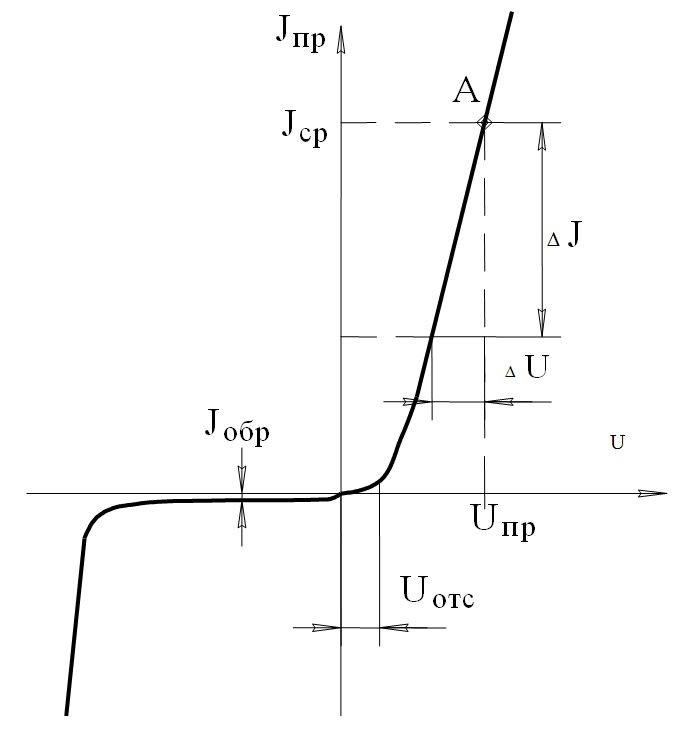
\includegraphics[width=0.4\textwidth]{2_VAC_of_diod.png}
\caption{ВАХ выпрямительного диода}
\label{fig:2_VAC_of_diod}
\end{figure}

\subsection*{Диоды}

Диоды обладают односторонней проводимостью и служат: для выпрямления переменного тока, стабилизации тока и напряжения, формирования импульсов, для регулирования мощностей и т.д.

Выпрямительные диоды применяются для преобразования переменного тока в постоянный. Они делятся: на маломощные (до 0,3А), средней мощности (до 10А), мощные (более 1000А), низкочастотные (до 1кГц) и высокочастотные (до 100кГц).

Свойства выпрямительных диодов характеризуются ВАХ и параметрами, которые приводятся в справочной литературе. Основные параметры диодов: средний выпрямленный ток Jср, прямое падение напряжения Uпр, обратный ток диода при заданной температуре Jобр., напряжение отсечки Uотс., мощность рассеивания Ррас., рабочая частота fр. и др.

\subsection*{Стабилитроны}

Стабилитроны - это разновидность диодов, предназначенных для стабилизации напряжения. Вольт – амперная характеристика стабилитрона имеет вид. Рабочий участок характеристики АВ лежит в области электрического пробоя диода и характеризуется малым изменением напряжения Uст при значительных изменениях тока.

\subsection*{Стабисторы}

Стабисторы, как и стабилитроны, предназначены для стабилизации напряжения. Однако, в отличие от последних, рабочим участком у них является прямая ветвь вольт–амперной характеристики. Стабисторы работают при прямом напряжении и позволяют стабилизировать малые напряжения (0,35 -- 1,9 В).

\subsection*{Варикапы}

Варикапы – это полупроводниковые диоды, емкость которых меняется при изменении обратного напряжения.


% Вопрос 3 ------------------------------------------------------------
\section{Полупроводниковые транзисторы. Классификация. Область применения.}

Транзистор — радиоэлектронный компонент из полупроводникового материала, обычно с тремя выводами, позволяющий входным сигналом управлять током в электрической цепи. Обычно используется для усиления, генерации и преобразования электрических сигналов. В общем случае транзистором называют любое устройство, которое имитирует главное свойство транзистора - изменения сигнала между двумя различными состояниями при изменении сигнала на управляющем электроде. Далее на схеме приведена классификация.

\subsection*{Классификация транзисторов}

\begin{figure}[H]
\centering
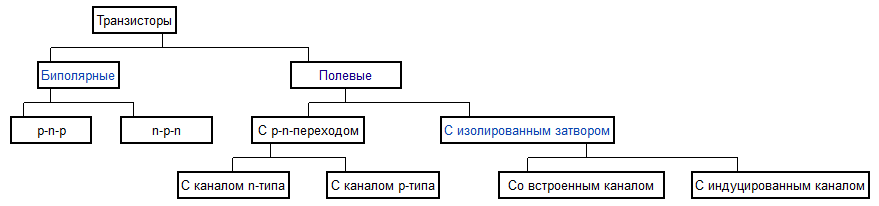
\includegraphics[width=1.0\textwidth]{3_Scheme_of_types.png}
\caption{Классификация транзисторов}
\label{fig:3_Scheme_of_types}
\end{figure}

\subsection*{Биполярный транзистор}

Принцип действия биполярного транзистора основан на использовании физических процессов, происходящих при переносе основных носителей электрических зарядов из эмиттерной области в коллекторную через базу.

$I_\text{э} = I_\text{к} + I_\text{б}$, где $I_\text{э}$, $I_\text{к}$, $I_\text{б}$, – токи соответственно в цепи эмиттера, коллектора, базы.

\subsection*{Полевой транзистор}

Полевым транзистором называется транзистор, в котором между двумя электродами образуется проводящий канал, по которому протекает ток. Управление этим током осуществляется электрическим полем, создаваемым третьим электродом. Электрод, с которого начинается движение носителей заряда, называется истоком, а электрод, к которому они движутся, стоком. Электрод, создающий управляющее электрическое поле, называется затвором.


% Вопрос 4 ------------------------------------------------------------
\section{Полупроводниковые резисторы. Классификация. Область применения.}

Полупроводниковые резисторы нашли широкое применение в электронных приборах. К ним относятся терморезисторы, магниторезисторы, варисторы, фоторезисторы. Принцип действия таких приборов основан на изменении свойств полупроводниковых материалов при воздействии на них температуры, магнитного и электрического полей, электромагнитного излучения.

Полупроводниковый терморезистор представляет собой прибор, сопротивление которого изменяется при изменении температуры. Зависимость сопротивления от температуры имеет вид:

\begin{equation}
R_{T}=A\exp{\frac{B}{T}}\text{, где}
\end{equation}
\par А, В --- постоянные, определяемые свойствами полупроводникового материала и конструкцией терморезистора;
\par Т --- температура.

С увеличением температуры сопротивление терморезистора уменьшается. Температурный коэффициент сопротивления терморезистора лежит в пределах от 2 до 8,5\% на градус.

Недостатком полупроводниковых терморезисторов является нелинейная зависимость сопротивления от температуры и значительный разброс параметров.

Терморезисторы применяются в качестве первичных преобразователей температуры для контроля и регулирования температуры, а также в схемах температурной компенсации.

Магниторезистор представляет собой полупроводниковый прибор, электрическое сопротивление которого зависит от воздействия на него магнитного поля. Магниторезисторы позволяют обеспечить хорошую гальваническую развязку. Для формирования магнитного поля можно использовать постоянный магнит или электромагнит.

Зависимость сопротивления магниторезистора от величины магнитного поля нелинейна. С увеличением величины магнитного поля сопротивление возрастает.

Основными параметрами магниторезистора являются:

\begin{itemize}
\item ном. сопротивление при отсутствии магнитного поля;
\item мощность рассеивания;
\item ТКR (температурный коэффициент сопротивления);
\item зависимость $R_{B} = f(H)$.
\end{itemize}


\begin{figure}[H]
\centering
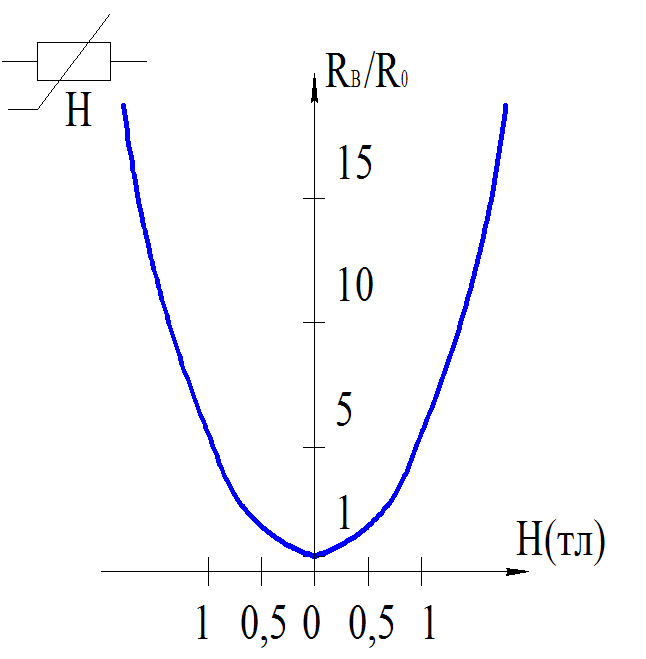
\includegraphics[width=0.35\textwidth]{4_R(H).png}
\hspace{1cm}
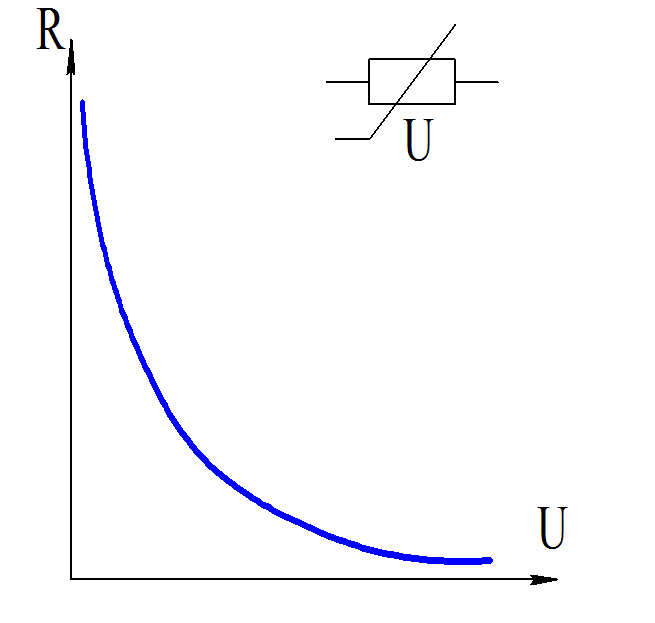
\includegraphics[width=0.35\textwidth]{4_R(U).png}
\\а) \hspace{0.4\textwidth} б)
\caption{Зависимости: R от H (а); R от U (б)}
\label{fig:4_R(U/H)}
\end{figure}

При увеличении магнитной индукции от 0 до 1 Тл сопротивление магниторезистора увеличивается в 10 - 15 раз. Магниторезисторы нашли применение в коммутационной технике: бесконтактных выключателях, реле, контактах управления. В настоящее время в приборостроении нашли широкое применение магнитодиоды, магнитотранзисторы, магнитотиристоры, которые представляют собой полупроводниковые приборы с p-n-переходами, параметры которых чувствительны к магнитному полю.

Варисторы представляют собой полупроводниковые резисторы, сопротивление которых зависит от приложенного напряжения. Зависимость сопротивления от напряжения нелинейная. Сопротивление RВ уменьшается при увеличении приложенного напряжения. Варисторы применяются для защиты от перенапряжений, защиты от помех, для искрогашения в электрических машинах. Они ограничивают возникающее напряжение, особенно при коммутации индуктивной или емкостной нагрузки и тем самым позволяют значительно повысить срок службы контактов реле и т.д.

Фоторезисторы представляют собой полупроводниковые приборы, сопротивление которых зависит от электромагнит. излучения.


% Вопрос 5 ----------------------------------------------------------
\section{Фотоэлектрические приборы. Классификация. Область применения.}

Фотоэлектрические приборы строятся на принципах фотопроводимости.

Фотопроводимость – это свойство веществ изменять свою электропроводность под воздействием электромагнитного излучения.

\subsection*{Классификация фотоэлектронных приборов}

\begin{enumerate}
\item с внешним фотоэффектом
	\begin{itemize}
	\item вакуумные
	\item газонаполненные фотоэлементы (ФЭ)
	\item фотоэлектронные умножители (ФЭУ)
	\end{itemize}
\item с внутренним фотоэффектом
	\begin{itemize}
	\item фоторезисторы
	\item фотодиоды
	\item фототранзисторы
	\item фототиристоры
	\end{itemize}
\end{enumerate}

В качестве излучателей используется солнечный свет, лампочки накаливания и другие источники света.

Фотоэлемент (ФЭ) – это электровакуумный или газоразрядный диод, в стеклянном баллоне которого установлены фотокатод и фотоанод. Фотокатод представляет собой слой, покрывающий внутреннюю поверхность колбы, выполненный из полупроводникового материала, чувствительного к внешнему излучению. Анод выполнен в виде кольца или рамки и размещен внутри колбы. ФЭ разделяются на вакуумные и газоразрядные.

При отсутствии излучения анодный ток равен нулю. При освещении фотокатода возникает фотоэмиссия, и в цепи анода протекает ток.

Фотоэлементы используются в первичных преобразователях информации.

\subsection*{Фотоэлектронный умножитель}

Фотоэлектронный умножитель представляет собой электровакуумный прибор, преобразующий энергию электромагнитного излучения в электрические сигналы с использованием вторичной электронной эмиссии. Состоит из стеклянного баллона, внутри которого расположены ускоряющие электроды, умножительные электроды и анод. При освещении фотокатода возникает электронный поток, который фокусируется и направляется на умножительные электроды, где за счет вторичной эмиссии он усиливается и попадает на анод.

\subsection*{Фоторезистор}

Фоторезистор представляет собой полупроводниковый прибор, сопротивление которого зависит от освещенности.

\subsection*{Фотодиод}

Фотодиод представляет собой полупроводниковый прибор с n-p переходом. Принцип работы фотодиода заключается в том, что при его освещении возрастает обратный ток, и он не зависит от обратного напряжения. На границе перехода “n-p” возникает ЭДС, величина которой зависит от освещенности и может достигать 0,5 - 1 В. При этом обратное сопротивление фотодиода уменьшается.

Они относятся к быстродействующим приборам и реагируют на сигналы до 1 МГц. Фотодиоды могут также использоваться в качестве источников питания, например, в солнечных батареях.

\subsection*{Фототранзистор}

Фототранзистор в отличие от фотодиода является активным преобразователем, в нем происходит не только преобразование энергии излучения, но и усиление.
Внутренний фотоэффект в полупроводнике может быть использован для построения других приборов, например, фототиристоров, однопереходных фототранзисторов и др.


% Вопрос 6 ----------------------------------------------------------------------
\section{Аналоговые усилители. Классификация. Основные характеристики и параметры.}

Усилитель - устройство, предназначенное для усиления электрических сигналов по напряжению, току или мощности за счет преобразования энергии источника питания в энергию выходного сигнала. Усилитель включает в себя нелинейный элемент, управляемый входным электрическим сигналом $U_\text{вх}$, источник питания $U_\text{п}$ и нагрузочное устройство с сопротивлением $Z_\text{н}$. Аналоговые усилители служат для усиления аналоговых сигналов.

\subsection*{Классификация усилителей}

\begin{itemize}
\item по виду усиливаемого:
	\begin{itemize}
	\item гармонических сигналов
	\item импульсных сигналов
	\end{itemize}
\item по типу усиливаемого сигнала:
	\begin{itemize}
	\item напряжения
	\item тока 
	\item мощности
	\end{itemize}
\item по диапазону усиливаемых частот:
	\begin{itemize}
	\item постоянного тока 
	\item переменного тока. Которые в зависимости от диапазона усиливаемых частот делятся на:
		\begin{itemize}
		\item усилители низкой частоты (УНЧ)
		\item высокой частоты (УВЧ)
		\item широкополосные
		\item избирательные усилители.
		\end{itemize}
	\end{itemize}
\item по виду нагрузки:
	\begin{itemize}
	\item с активной нагрузкой
	\item c активно-индуктивной нагрузкой
	\item c емкостной нагрузкой
	\end{itemize}
\item по количеству каскадов:
	\begin{itemize}
	\item однокаскадные 
	\item многокаскадные. Связь в между каскадами может быть:
		\begin{itemize}
		\item гальванической
		\item емкостной
		\item индуктивной
		\end{itemize}
	\end{itemize}
\end{itemize}

\subsection*{Основные характеристики усилителя}

\begin{itemize}
\item амплитудная характеристика, которая представляет собой зависимость $U_\text{выx} = \varphi(U_\text{вх})$. Для линейных усилителей это прямая, проходящая через начало координат;
\item амплитудно-частотная характеристика (АЧХ) $U_\text{выx} = \varphi(f)$ отражает зависимость амплитуды выходного сигнала от частоты. Реально в усилителях из-за наличия паразитных емкостей и индуктивностей различные частоты усиливаются неодинаково;
\item фазо-частотная характеристика $U_\text{выx} = \lambda(f)$ отражает зависимость угла сдвига фазы выходного сигнала по отношению к фазе входного сигнала;
\item переходная характеристика – отражает реакцию усилителя на единичный скачок входного напряжения. Переходная характеристика определяется по ее изображению на экране осциллографа при подаче на вход усилителя входного сигнала прямоугольной формы. Процесс изменения выходного сигнала может быть колебательным либо апериодичным.
\end{itemize}

\subsection*{Важнейшие параметры усилителя}

\begin{itemize}
\item коэффициент усиления по току $K_{I} = \dfrac{\Delta I_\text{вых}}{\Delta I_\text{вх}}$
\item коэффициент усиления по напряжению $K_{U} = \dfrac{\Delta U_\text{вых}}{\Delta U_\text{вх}}$
\item коэффициент усиления по мощности $K_{P} = \dfrac{\Delta P_\text{вых}}{\Delta P_\text{вх}}$
\item Полоса пропускания усилителя $2\Delta f$ характеризует частотные свойства усилителя. Измеряется на уровне $0,707 K_{max}$
\end{itemize}

Для наглядности в ряде случаев АЧХ строится в относительных единицах усиления.
\begin{equation}
N(F) = \dfrac{K(f)}{K_{max}}\text{, где}
\end{equation}
\par $K(f)$ --- коэффициент усиления на частоте $f$;
\par $K_{max}$ --- максимальный коэффициент усиления.

Входное и выходное сопротивление необходимо учитывать при согласовании с источником входного сигнала и с нагрузкой. 

Выходная мощность усилителя – это мощность, которая выделяется на нагрузке.

Искажения сигналов в усилителе – это отклонение формы выходного сигнала от формы входного сигнала. Различают два вида искажений: статические (нелинейные) и динамические (линейные). Нелинейные искажения возникают в усилителе за счет работы его на нелинейном участке ВАХ. Количественно нелинейные искажения оцениваются коэффициентом нелинейных искажений.

\begin{equation}
K_{H} = \dfrac{\sqrt{(A_{2}^{2} + A_{3}^{2} + \ldots + A_{n}^{2})} }{A_{1}}\text{, где}
\end{equation}
\par $A_{n}$ --- амплитуда n-й гармоники;
\par $A_{1}$ --- амплитуда основной гармоники выходного сигнала.

Линейные искажения определяются амплитудно-частотной характеристикой усилителя и количественно оцениваются коэффициентами частотных искажений на низких и высоких частотах.

Для получения высоких коэффициентов усиления в состав усилителя входит обычно несколько каскадов. Первым каскадом, как правило, является предварительный усилитель, затем идут промежуточный усилитель и усилитель мощности. Предварительный усилитель обеспечивает связь источника сигнала с усилителем. Он должен иметь большое входное сопротивление для того, чтобы не ослаблять входной сигнал. Промежуточный усилитель обеспечивает основное усиление, а усилитель мощности обеспечивает заданную выходную мощность.

При построении усилительных устройств наибольшее распространение получили каскады на биполярных и полевых транзисторах, включенных с ОЭ (OU) или с ОК (OC).

% Вопрос 7 -----------------------------------------------------------------------------------------
\section{Избирательные усилители. Усилители постоянного тока. Усилители мощности. Область применения.}

Избирательными называются усилители, усиливающие сигналы в относительно узкой полосе частот. Основными показателями избирательных усилителей являются максимальный коэффициент усиления, полоса пропускания, средняя частота полосы пропускания и избирательность. Основным требованием, предъявляемым к избирательным усилителям, является получение высокой избирательности, которая определяется крутизной склонов его амплитудно-частотной характеристики. Чем круче спады частотной характеристики и чем меньше коэффициент усиления усилителя за пределами полосы пропускания, тем выше его избирательность. Избирательность таких усилителей оценивают величиной коэффициента прямоугольности АЧХ, который равен отношению ширины полосы пропускания на уровне 0,7 к ширине полосы на уровне 0,1 (или к ширине полосы на уровне 0,01):

\begin{equation}
K_\text{п} = \dfrac{2\Delta f_{0,7}}{2\Delta f_{0,01 - 0,1}}
\end{equation}

Избирательные усилители применяются в основном для усиления сигналов высокой частоты и разделяются на два вида: резонансные усилители и полосовые усилители. В резонансных усилителях нагрузкой обычно является одиночный параллельный колебательный контур. Перестраивая контур, можно изменять резонансную частоту в некоторых пределах.

Полосовые усилители обеспечивают амплитудно-частотную характеристику по форме близкую к прямоугольной. Полосовые усилители не перестраиваются и работают на фиксированных частотах. В качестве нагрузки они имеют один или два колебательных контура в каждом каскаде. В усилителях промежуточной частоты радиоприемников применяются также фильтры сосредоточенной селекции, состоящие из трех-четырех связанных колебательных контуров. В качестве фильтров сосредоточенной селекции также широко применяются пьезоэлектрические фильтры. В них благодаря прямому и обратному пьезоэлектрическому эффекту амплитудно-частотная характеристика формируется в системе из нескольких механических резонаторов.

Однокаскадный резонансный усилитель состоит из активного элемента, нагрузкой которого является одиночный параллельный колебательный контур. В качестве активного элемента можно использовать биполярные или полевые транзисторы, включаемые, чаще всего, по схеме с общим эмиттером или общим истоком. При этом колебательный контур оказывается зашунтированным выходным сопротивлением собственного каскада и входным сопротивлением следующего каскада в многокаскадном усилителе, за счет чего избирательность ухудшается. В каскадах с полевым транзистором колебательный контур шунтируется слабо, так как входное и выходное сопротивление полевого транзистора достаточно большое. В таких каскадах возможно полное включение контура в нагрузочную цепь. Биполярные транзисторы имеют относительно малые значения входных и выходных сопротивлений. Поэтому при непосредственном включении колебательного контура в нагрузочную цепь контур шунтируется значительно сильнее и его избирательные свойства заметно ухудшаются. Поэтому в резонансных каскадах на биполярных транзисторах принимают специальные меры для уменьшения шунтирующего действия входного и выходного сопротивления транзистора. С этой целью ослабляют связь транзистора с колебательным контуром, используя частичное включение контура в нагрузочную цепь. В связи с тем, что резонансные избирательные усилители работают на высокой частоте, существенное влияние на их работу может оказывать внутренняя обратная связь, имеющаяся между входом и выходом в любом активном элементе. Эта внутренняя обратная связь на одной из высоких частот может оказаться положительной, что приведет к нарушению устойчивой работы усилителя и его самовозбуждению. Для повышения устойчивости работы каскада необходимо ослаблять связь его активного элемента с колебательным контуром. С этой целью частичное включение контура используют и в резонансных каскадах на полевых транзисторах. Далее на рисунке показана схема резонансного усилителя на полевом транзисторе с полным включением контура и его АЧХ.

\subsection*{Схема на полевом транзисторе}

Модуль коэффициента усиления каскада на полевом транзисторе при полном включении контура примерно равен:

\begin{equation}
|K_\text{рез}| \approx S R_\text{рез}
\end{equation}
где $ R_\text{рез} = Q\rho $ - сопротивление параллельного контура на резонансной частоте.

\begin{figure}[H]
\centering
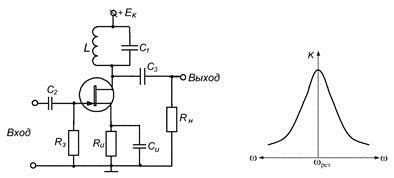
\includegraphics[width=0.6\textwidth]{7_field_based_amp.jpg}
\caption{Избирательный усилитель на полевом транзисторе и его АЧХ}
\label{fig:7_field_based_amp}
\end{figure}

\subsection*{Схема на биполярном транзисторе}

Далее показана схема избирательного усилителя на биполярном транзисторе с неполным включением контура. Для каскада на биполярном транзисторе при неполном включении контура в цепь нагрузки необходимо учитывать коэффициенты подключения контура и модуль коэффициента усиления будет определяться следующим выражением:

\begin{equation}
|K_\text{рез}| = b_{1}b_{2} \dfrac{\beta R_\text{рез}}{R_\text{вх}}
\end{equation}
где $ b_{1} = \dfrac{L\prime}{L} $ и $ b_{2} = \dfrac{L\prime\prime}{L} $ - коэффициенты включения контура; $L$ - полная индуктивность катушки; $L\prime$ - индуктивность части катушки, к которой подключен коллектор транзистора; $L\prime\prime$ - индуктивность части катушки, с которой усиленный сигнал снимается на вход следующего каскада.

\begin{figure}[H]
\centering
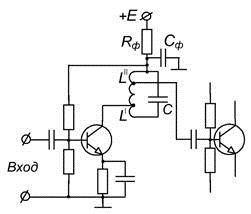
\includegraphics[width=0.4\textwidth]{7_bipolar_based_amp.jpg}
\caption{Избирательный усилитель на биполярном транзисторе}
\label{fig:7_bipolar_based_amp}
\end{figure}

\subsection*{2T-мост}

При необходимости избирательного усиления низких частот емкости и индуктивности колебательного контура должны быть большими и добротность контура оказывается низкой при значительном увеличении габаритов катушки и конденсатора. Поэтому в качестве низкочастотных избирательных усилителей используют усилители с частотно-зависимой отрицательной обратной связью. В качестве частотно-зависимой цепи используют двойной T-образный мост (2T-мост).

\begin{figure}[H]
\centering
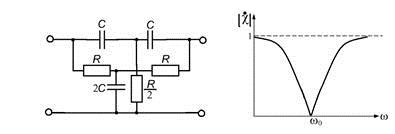
\includegraphics[width=0.6\textwidth]{7_2T.jpg}
\caption{Схема 2T-моста и АХЧ}
\label{fig:7_2T}
\end{figure}

Если включить 2T-мост в цепь отрицательной обратной связи в RC-усилитель, то поскольку на частоте $\omega = \omega_{0}$ коэффициент передачи моста равен нулю, отрицательная обратная связь будет отсутствовать, и коэффициент усиления усилителя будет максимальным. На всех остальных частотах коэффициент усиления избирательно уменьшается из-за наличия отрицательной обратной связи. В результате амплитудно-частотная характеристика усилителя с 2T-мостом в цепи отрицательной обратной связи будет иметь ярко выраженный максимум на частоте $\omega_{0}$.

\begin{figure}[H]
\centering
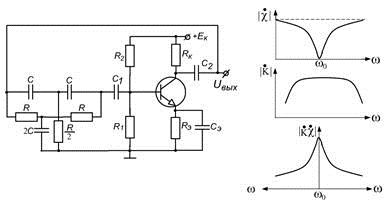
\includegraphics[width=0.6\textwidth]{7_2T_with_feedback.jpg}
\caption{Схема 2T-моста с обратной связью и АХЧ}
\label{fig:7_2T_with_feedback}
\end{figure}

Схема избирательного усилителя с 2T-мостом эквивалентна резонансному каскаду, имеющему добротность $Q = \dfrac{K}{4}$ , где $K$- коэффициент усиления усилителя без обратной связи. Для увеличения эквивалентной добротности избирательной системы можно цепью отрицательной обратной связи через 2Т-мост охватывать несколько каскадов усиления.

\subsection*{Усилители постоянного тока}

Усилителями постоянного тока называют такие устройства, которые могут усиливать медленно изменяющиеся электрические сигналы, то есть они способны усиливать и переменные и постоянные составляющие входного сигнала. Усилители постоянного тока имеют много разновидностей (дифференциальные, операционные, усилители с преобразованием входного сигнала и др.). Поскольку такие устройства пропускают наряду с переменной составляющей еще и постоянную, то отдельные каскады должны быть связаны между собой либо непосредственно, либо через резисторы, но не через разделительные конденсаторы или трансформаторы, которые не пропускают постоянную составляющую. Основную проблему усилителей постоянного тока представляет дрейф нуля – отклонение напряжения на выходе усилителя от начального (нулевого) значения при отсутствии входного сигнала. Основной причиной этого явления являются температурная и временная нестабильность параметров активных элементов схемы усилителя, резисторов, а также источников питания. Одним из возможных путей уменьшения дрейфа нуля является использование дифференциальных усилителей.

\begin{itemize}
\item Дифференциальные усилители предназначены для усиления сколь угодно медленно изменяющихся во времени сигналов, частотный диапазон которых начинается от 0 Гц.
\item Дифференциальный усилитель: имеет следующие достоинства: малый дрейф нуля; высокая степень подавления синфазных помех.
\item Недостатки дифференциального усилителя: требует двухполярного источника питания; необходима очень высокая симметрия схемы.
\end{itemize}

\begin{figure}[H]
\centering
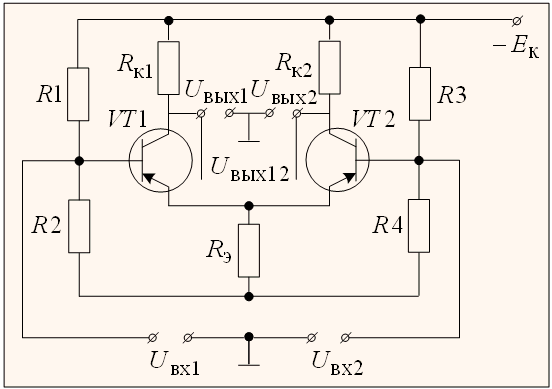
\includegraphics[width=0.5\textwidth]{7_diff_amp.png}
\caption{Схема простейшего дифференциального усилителя}
\label{fig:7_diff_amp}
\end{figure}

\begin{itemize}
\item Дифференциальные усилители предназначены для усиления сколь угодно медленно изменяющихся во времени сигналов, частотный диапазон которых начинается от 0 Гц.
\item Дифференциальный усилитель: имеет следующие достоинства: малый дрейф нуля; высокая степень подавления синфазных помех.
\item Недостатки дифференциального усилителя: требует двухполярного источника питания; необходима очень высокая симметрия схемы.
\end{itemize}


% Вопрос 8 ------------------------------------------------------------------------
\section{Операционные усилители. Классификация. Область применения. Балансировка ОУ.}

Операционным усилителем называют усилитель постоянного тока, предназначенный для выполнения различного рода операций над аналоговыми сигнала при работе в схемах с отрицательной обратной связью.

Операционные усилители обладают большим и стабильным коэффициентом усиления напряжения, имеют дифференциальный вход с высоким входным сопротивлением и несимметричный выход с низким выходным сопротивлением, малым дрейфом нуля. То есть под операционным усилителем понимают высококачественный универсальный усилитель.

Условные обозначения операционных усилителей приведены ниже. Один из входов, обозначенный знаком «+» называют неинвертирующим (прямым), так как сигнал на выходе и сигнал на этом входе имеют одинаковую полярность. Второй вход, обозначенный знаком «–», (его также обозначают знаком инверсии «o») называют инвертирующим, так как сигнал на выходе по отношению к сигналу на этом входе имеет противоположную полярность. Помимо трех сигнальных контактов (двух входных и одного выходного) операционный усилитель содержит дополнительные контакты (обычно число контактов составляет 14 или 16).

\begin{figure}[H]
\centering
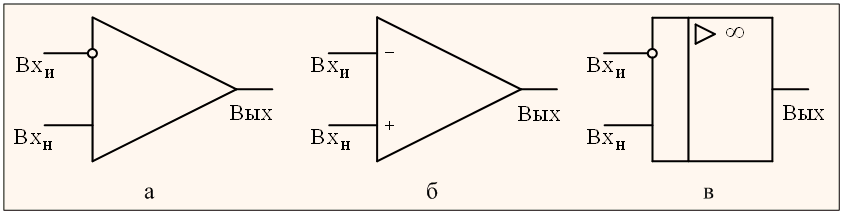
\includegraphics[width=0.7\textwidth]{8_oa_graphic.png}
\caption{УГО операционного усилителя}
\label{fig:8_oa_graphic}
\end{figure}

\subsection*{Основные параметры}

\begin{enumerate}
\item Коэффициент усиления напряжения без обратной связи $K_{u}$, показывающий, во сколько раз напряжение на выходе превышает напряжение сигнала, поданного на дифференциальный вход. Типовое значение $K_{u} = 10^{5} \div 10^{6}$;
\item Коэффициент ослабления синфазного сигнала $K_\text{осл.сф}$, показывающий, во сколько раз дифференциальный сигнал сильнее синфазного. Донный параметр определяется свойствами входного дифференциального каскада и составляет $80 \div 100$ дБ;
\item Напряжение смещения нуля $U_\text{см}$, представляющее собой постоянное напряжение определенной полярности, которое необходимо подать на вход при отсутствии входного сигнала для того, чтобы напряжение на выходе стало равным нулю. Наличие отклонения выходного напряжения от нуля обусловлено, хотя и малым, но неизбежным дисбалансом плеч дифференциального каскада. Практически $U_\text{см} = 5 \div 20$ мВ;
\item Температурный дрейф напряжения смещения $TKU_\text{см} = \dfrac{\Delta U_\text{см}}{\Delta T}$, характеризует изменение напряжения $U_\text{см}$ при изменении температуры и составляет $1 \div 30 \dfrac{\text{мкВ}}{\text{\textcelsius}}$;
\item Входное сопротивление для дифференциального сигнала $R_\text{вх. диф}$. Измеряется со стороны любого входа в то время, когда другой вход соединен с общим выводом. Величина $R_\text{вх. диф}$ лежит в пределах сотен кОм – единиц МОм;
\item Входное сопротивление для синфазного сигнала $R_\text{вх. сф}$. Измеряется между соединенными вместе входами операционного усилителя и корпусом. Данное сопротивление на несколько порядков больше чем сопротивление для дифференциального сигнала;
\item Выходное сопротивление $R_\text{вых}$. Величина выходного сопротивления для операционного усилителя составляет десятки – сотни Ом.
\end{enumerate}

\subsection*{Виды ОУ}

\begin{enumerate}
\item Универсальные усилители общего назначения составляют большую часть номенклатуры ОУ. Это дешевые усилители среднего быстродействия, невысокой точности и малой выходной мощности, с  типичными параметрами: Ku = $10^{3} - 10^{5}$, f1 = 0.1 - 10 МГц и напряжение смещения нулевого уровня Uсм = 0.1 - 10 мВ.
\item Прецизионные усилители характеризуются суммарной погрешностью не более долей процента и при среднем быстродействии имеют высокий коэффициент усиления напряжения, малое напряжение смещения нуля, большой коэффициент подавления синфазного сигнала, малый входной ток и низкий уровень шума.
\item Быстродействующие усилители имеют высокую частоту единичного усиления f1 = 50 - 1000 МГц и обеспечивают скорость нарастания выходного сигнала Vu= 10 - 1000 В/мкс при средних точностных параметрах.
\item Микромощные усилители потребляют очень малый ток Iпит порядка 1 мкА при небольших уровнях напряжения электропитания Uпит = $\pm 0.9 - \pm 5$ В. Все другие параметры (особенно быстродействие) у них обычно невысокие. Эти усилители используют в приборах с автономным электропитанием от гальванических или аккумуляторных батарей.
\item Мощные и высоковольтные усилители имеют разность положительного и отрицательного питающих напряжений свыше 50 В и выходной ток 0.1 - 1А, а некоторые модификации допускают токи до 10 - 100 А и мощности свыше 100 Вт.
\end{enumerate}

\subsection*{Балансировка ОУ}

Балансировка ОУ представляет собой операцию по компенсации напряжения смещения в ОУ. Балансировка производится с помощью многооборотного потенциометра Rб , начало и конец которого подключены на входы R ОУ, а средний вывод - на источник питания Un (-Un). Для балансировки входы ОУ заземляются, и с помощью потенциометра Rб устанавливается напряжение Uвых = 0. Балансировка позволяет компенсировать напряжение смещения ОУ в данный момент при действующих дестабилизирующих факторах. При изменении параметров питающих напряжений и внешних факторов, таких как температура и влажность окружающей среды, балансировка нарушается. Поэтому в ряде случаев применяется автоматическая установка нулей ОУ.

% Вопрос 9 --------------------------------------------------------------------
\section{Стабилизаторы напряжения. Классификация. Параметры. Область применения.}

Стабилизатор напряжения — преобразователь электрической энергии, позволяющий получить на выходе напряжение, находящееся в заданных пределах при значительно больших колебаниях входного напряжения и сопротивления нагрузки.

По типу выходного напряжения стабилизаторы делятся на стабилизаторы постоянного тока и переменного тока. Как правило, тип питания (постоянный либо переменный ток) такой же, как и выходное напряжение, хотя возможны исключения.

Стабилизаторы напряжения подразделяются на однофазные и трехфазные стабилизаторы напряжения.

\subsection*{Классификация стабилизаторов по конструкции}

\begin{itemize}
\item феррорезонансные. Принцип действия основывается на магнитном насыщении сердечников из ферромагнетиков трансформаторов. Этот тип стабилизаторов напряжения был разработан достаточно давно, в начале 60-х годов прошлого века и был призван защитить сложную бытовую технику. Но в настоящее время от их производства отказались почти все производители, из-за очень узкого рабочего диапазона напряжений и невозможности работы прибора без нагрузки.
\item электромеханические. В стабилизаторах этого типа корректировка напряжения производится автоматически, а точность поддержания напряжения достаточно высока (в пределах 3\%).
\item электронные. Этот тип стабилизаторов работает по принципу автоматического переключения трансформаторных секций при помощи силовых ключей (реле, тиристоров и т.д.). Электронные стабилизаторы ступенчатого регулирования обеспечивают выходное напряжение в более широких пределах, чем электромеханические. А также обладают высоким быстродействием и не изменяют форму входного напряжения.
\end{itemize}

\subsection*{Основные параметры стабилизатора}

\begin{itemize}
\item Диапазон входных напряжений(Диапазон напряжений в пределах которого стабилизатор может поддерживать выходное напряжение с заданной точностью)
\item Диапазон  выходных напряжений (Диапазон возможных значений)
\item Точность поддержания выходного напряжения в \%
\item Мощность стабилизатора. Обычно указывается в кВа, это полная мощность.
\end{itemize}

\subsection*{Выбор стабилизатора}

\begin{enumerate}
\item Для выбора стабилизатора необходимо посчитать сумму полных мощностей потребителей, если на потребителе указан $\cos\varphi$ (коэфф. активном мощности в полной), то его учитываем.
\item Определить диапазон изменений напряжений в сети. Произвести изменения максимальных и минимальных напряжений.
\item Выяснить диапазон рабочих напряжений потребителей
\end{enumerate}


% Вопрос 10 ------------------------------------
\section{Логические операции. Схемная реализация.}

Логическая операция — операция над выражениями булевского типа, соответствующая некоторой операции над высказываниями в алгебре логики. Как и высказывания, логические выражения могут принимать одно из двух истинностных значений — «истинно» или «ложно». Логические операции служат для получения сложных логических выражений из более простых. В свою очередь, логические выражения обычно используются как условия для управления последовательностью выполнения программы.
Обычно выделяют следующие базовые операции:

\begin{itemize}
\item НЕ (отрицание)
\item И (конъюнкция)
\item ИЛИ (дизъюнкция)
\item XOR (исключающее ИЛИ)
\end{itemize}

Для каждой из операции можно построить простую таблицу истинности.

\begin{figure}[H]
\centering
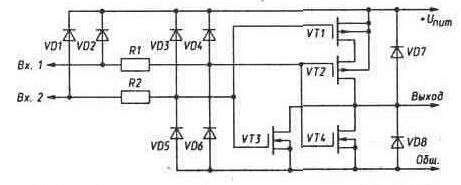
\includegraphics[width=0.7\textwidth]{10_or_not.png}
\caption{Схемная реализация ИЛИ-НЕ}
\label{fig:10_or_not}
\end{figure}

Для всех микросхем существует УГО.


% Вопрос 11 ---------------------------------------------------------------------------------------------------------------
\section{Цифровые устройства. Классификация. Комбинационные ЦУ. Дешифраторы, шифраторы, мультиплексоры, демультиплексоры.}

\subsection*{Виды цифровых устройств}

\begin{enumerate}
\item Логические элементы
\item Триггеры
\item Счётчики
\item Регистры
\item Буферные преобразователи
\item Модули памяти
\item Шифраторы
\item Дешифраторы
\item Цифровой компаратор
\item Мультиплексоры
\item Демультиплексоры
\item Полусумматоры
\item Сумматоры
\item АЛУ
\item Микроконтроллеры
\item (Микро)процессоры
\item Однокристальные микрокомпьютеры
\item ПЛИС — программируемые логические интегральные схемы
\end{enumerate}

\subsection*{Классификация цифровых устройств}

\begin{itemize}
\item В зависимости от способа  ввода и вывода информации:
	\begin{itemize}
	\item Последовательные – в котором входные сигналы поступают на вход, а выходные сигналы снимаются с выхода последовательно, разряд за разрядом;
	\item Параллельные – входные сигналы подаются на вход, а выходные снимаются с выхода одновременно;
	\item Последовательно-параллельные – входные и выходные сигналы представлены в разных формах: либо на вход сигналы поступают последовательно сигнал за сигналом, а с выхода они снимаются одновременно, и наоборот.
	\end{itemize}
\item По принципу действия:
	\begin{itemize}
	\item КЦУ (комбинационные цифр.устр-ва) – выходные сигналы которых определяются только действующими в данный момент входными сигналами и не зависят от внутреннего состояния устройства.
	\item Последовательными – выходные сигналы которых зависят не только от входных сигналов, но и от внутреннего состояния устройства. Этот тип называют цифровыми автоматами.
	\end{itemize}
\end{itemize}

\subsection*{Виды комбинационных ЦУ}
\begin{itemize}
\item дешифраторы
\item шифраторы
\item мультиплексоры
\item демультиплексоры
\item комбинационные сумматоры
\item АЛУ
\end{itemize}


\subsection*{Дешифратор}

Дешифратором называется комбинационная цифровая схема с несколькими входами и выходами, преобразующая код, подаваемый на входы, в сигнал на одном из выходов. Если дешифратор, имеющий n входов, имеет $2^{n}$ выходов, то такой дешифратор называется полным. Если количество выходов меньше, то дешифратор называется неполным.
\begin{figure}[H]
\centering
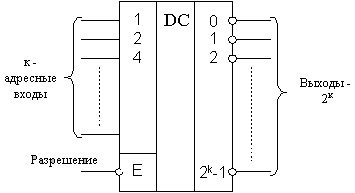
\includegraphics[width=0.5\textwidth]{11_dc.png}
\caption{УГО дешифратора}
\label{fig:11_dc}
\end{figure}

\subsection*{Шифратор}

Шифратором называется устройство, предназначенное для преобразования чисел из десятичной системы в двоичную. Нетрудно видеть, что в шифраторе сигнал, подаваемый на вход X0, не используется. Основное применение шифраторов - это введение первичной информации с клавиатуры (преобразование десятичного в ДВОИЧНЫЙ), например, ИС К555ИВЗ.
\begin{figure}[H]
\centering
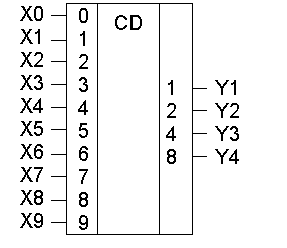
\includegraphics[width=0.4\textwidth]{11_cd.png}
\caption{УГО шифратора}
\label{fig:11_cd}
\end{figure}

\subsection*{Мультиплексор}

Мультиплексором называется комбинационное цифровое устройство, предназначенное для управляемой передачи информации с нескольких источников в один выходной канал. Мультиплексор можно реализовать, используя логические элементы "И" и дешифратор. Мультиплексор имеет один выход, информационные входы и адресные или управляющие входы. В зависимости от кода, подаваемого на адресные шины Х0, Х1 один из информационных входов подключается к выходному каналу.
\begin{figure}[H]
\centering
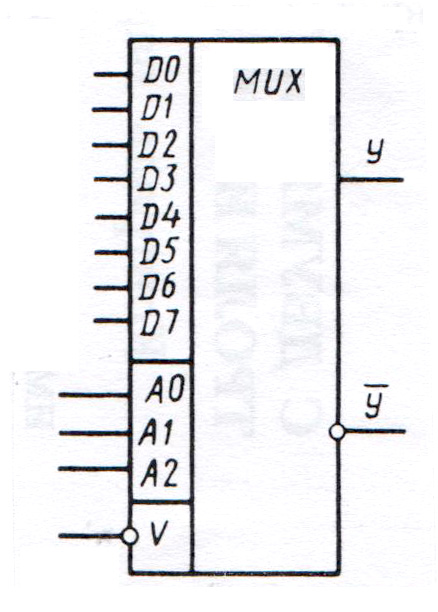
\includegraphics[width=0.25\textwidth]{11_ms.jpg}
\caption{УГО мультиплексора}
\label{fig:11_ms}
\end{figure}

\subsection*{Демультиплексор}

Демультиплексором называется комбинационное логическое устройство, предназначенное для управляемой передачи данных от одного источника информации в несколько выходных каналов. Демультиплексор имеет один информационный вход, n адресных шин и $2^{n}$-выходов.
\begin{figure}[H]
\centering
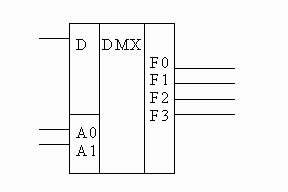
\includegraphics[width=0.45\textwidth]{11_dmx.png}
\caption{УГО демультиплексора}
\label{fig:11_dmx}
\end{figure}


% Вопрос 12 ---------------------------------------------------------------------------------------------------------------
\section{Комбинационные сумматоры.}

Комбинационный сумматор - это цифровое устройство, пред-назначенное для арифметического сложения чисел, представленных в виде двоичных кодов.

Обычно сумматор представляет собой комбинацию одноразрядных сумматоров. При сложении двух чисел в каждом разряде производится сложение трех цифр: цифры первого слагаемого Ai, цифры второго слагаемого Bi; и цифры переноса из младшего разряда Рi;. В результате суммирования на выходных шинах получается сумма S; и перенос в старший разряд Pj+i.

\begin{figure}[H]
\centering
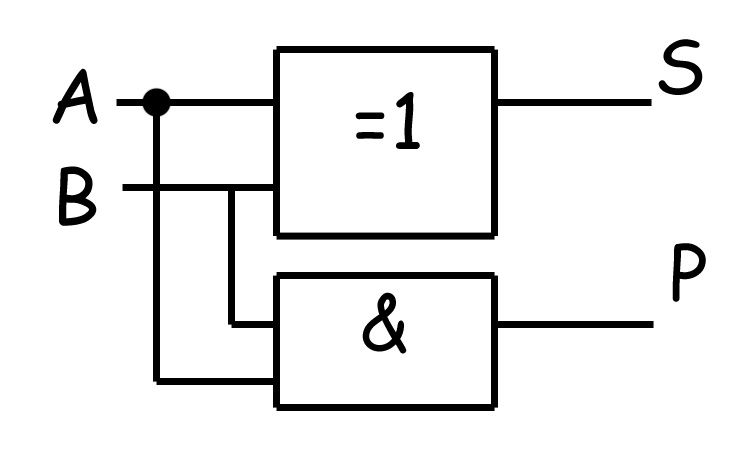
\includegraphics[width=0.3\textwidth]{12_additor.jpg}
\caption{Структура простейшего сумматора}
\label{fig:12_additor}
\end{figure}

\begin{figure}[H]
\centering
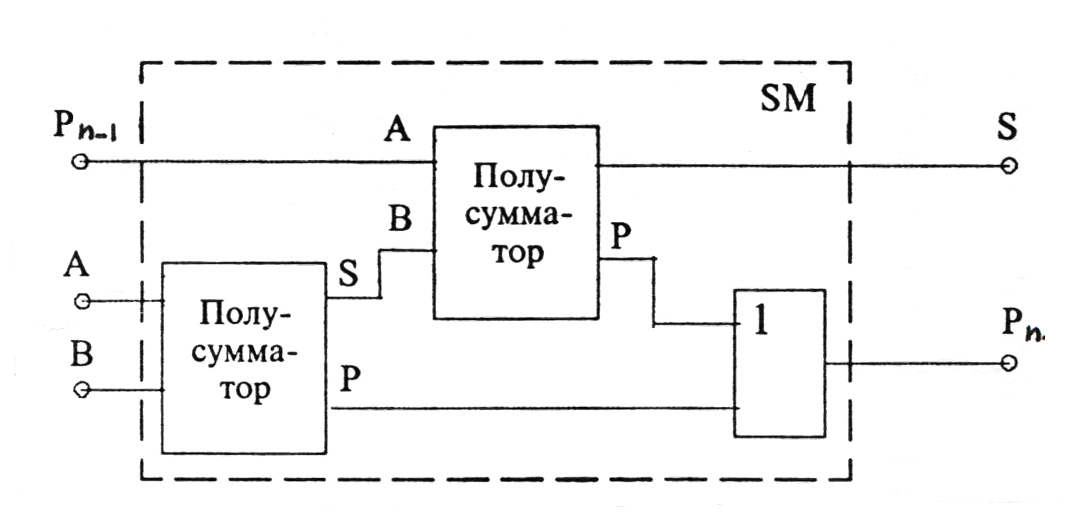
\includegraphics[width=0.7\textwidth]{12_cs.jpg}
\caption{Структура комбинационного сумматора}
\label{fig:12_cs}
\end{figure}


% Вопрос 13 ---------------------------------------------------------------------------------------------------------------
\section{Триггера. Классификация. Область применения.}

Триггером называется цифровое устройство, которое может находиться в одном из двух устойчивых состояний и переходит из одного состояния в другое под действием входных сигналов. Триггеры можно классифицировать по способу приема информации, принципу построения, функциональным возможностям. По способу приема информации триггеры подразделяются на асинхронные и синхронные. Асинхронный триггер изменяет свое состояние в момент прихода сигнала на его информационные входы. Синхронные триггеры изменяют свое состояние под воздействием входных сигналов только в момент прихода активного сигнала на его синхронизирующий вход С.

По виду активного сигнала, действующего на информационных входах, триггеры подразделяются на статические и динамические. Первые переключаются потенциалом (уровнем напряжения), а вторые – перепадом (передним или задним фронтом импульса). Входные информационные сигналы могут быть прямыми и инверсными.

\subsection*{Асинхронный RS-триггер}

RS-триггер — триггер, который сохраняет своё предыдущее состояние при нулевых входах и меняет своё выходное состояние при подаче на один из его входов единицы.

Таблица истинности асинхронного RS-триггера.

\begin{tabular}{|c|c|c|}
\hline	S	& R	& Q			\\
\hline	0	& 0	& Q(n-1)	\\
\hline	0	& 1	& 0			\\
\hline	1	& 0	& 1			\\
\hline	1	& 1	& X			\\
\hline
\end{tabular}

\subsection*{Синхронный RS-триггер}

Синхронный RS-триггер очень похож на асинхронный, с тем лишь различием, что имеется вход синхронизации, при 1 на котором и происходит работа.

Таблица истинности синхронного RS-триггера.

\begin{tabular}{|c|c|c|c|c|}
\hline	C	& S	& R	& Q(t)	& Q(t+1)	\\
\hline	0	& X	& X	& 0		& 0			\\
\hline	0	& X	& X	& 1		& 1			\\
\hline	1	& 0	& 0	& 0		& 0			\\
\hline	1	& 0	& 0	& 1		& 1			\\
\hline	1	& 0	& 1	& 0		& 0			\\
\hline	1	& 0	& 1	& 1		& 0			\\
\hline	1	& 1	& 0	& 0		& 1			\\
\hline	1	& 1	& 0	& 1		& 1			\\
\hline	1	& 1	& 1	& 0		& не опред.	\\
\hline	1	& 1	& 1	& 1		& не опред.	\\
\hline
\end{tabular}

\subsection*{D-триггер}

D-триггер — запоминает состояние входа и выдаёт его на выход. D-триггеры имеют, как минимум, два входа: информационный D и синхронизации С. После прихода активного фронта импульса синхронизации на вход С D-триггер открывается. Сохранение информации в D-триггерах происходит после спада импульса синхронизации С. Так как информация на выходе остаётся неизменной до прихода очередного импульса синхронизации, D-триггер называют также триггером с запоминанием информации или триггером-защёлкой. Рассуждая чисто теоретически, парафазный (двухфазный) D-триггер можно образовать из любых RS- или JK-триггеров, если на их входы одновременно подавать взаимно инверсные сигналы.

D-триггер в основном используется для реализации защёлки. Так, например, для снятия 32 бит информации с параллельной шины, берут 32 D-триггера и объединяют их входы синхронизации для управления записью информации в защёлку, а 32 D входа подсоединяют к шине.

В одноступенчатых D-триггерах во время прозрачности все изменения информации на входе D передаются на выход Q. Там, где это нежелательно, нужно применять двухступенчатые (двухтактные, Master-Slave, MS) D-триггеры.

Таблица истинности синхронного D-триггера.

\begin{tabular}{|c|c|c|}
\hline	D	& Q(t)	& Q(t+1)	\\
\hline	0	& 0		& 0			\\
\hline	0	& 1		& 0			\\
\hline	1	& 0		& 1			\\
\hline	1	& 1		& 1			\\
\hline
\end{tabular}

\subsection*{T-триггер}

Синхронный Т-триггер, при единице на входе Т, по каждому такту на входе С изменяет своё логическое состояние на противоположное, и не изменяет выходное состояние при нуле на входе T. Т-триггер можно построить на JK-триггере, на двухступенчатом (Master-Slave, MS) D-триггере и на двух одноступенчатых D-триггерах и инверторе.

Как можно видеть в таблице истинности JK-триггера, он переходит в инверсное состояние каждый раз при одновременной подаче на входы J и K логической 1. Это свойство позволяет создать на базе JK-триггера Т-триггер, объединяя входы J и К.

В двухступенчатом (Master-Slave, MS) D-триггере инверсный выход Q соединяется со входом D, а на вход С подаются счётные импульсы. В результате триггер при каждом счётном импульсе запоминает значение Q, то есть будет переключаться в противоположное состояние.

Т-триггер часто применяют для понижения частоты в 2 раза, при этом на Т вход подают единицу, а на С — сигнал с частотой, которая будет поделена на 2.

Таблица истинности синхронного T-триггера.

\begin{tabular}{|c|c|c|}
\hline	T	& Q(t)	& Q(t+1)	\\
\hline	0	& 0		& 0			\\
\hline	0	& 1		& 1			\\
\hline	1	& 0		& 1			\\
\hline	1	& 1		& 0			\\
\hline
\end{tabular}

\subsection*{JK-триггер}

JK-триггер работает так же как RS-триггер, с одним лишь исключением: при подаче логической единицы на оба входа J и K состояние выхода триггера изменяется на противоположное. Вход J (от англ. Jump — прыжок) аналогичен входу S у RS-триггера. Вход K (от англ. Kill — убить) аналогичен входу R у RS-триггера. При подаче единицы на вход J и нуля на вход K выходное состояние триггера становится равным логической единице. А при подаче единицы на вход K и нуля на вход J выходное состояние триггера становится равным логическому нулю. JK-триггер в отличие от RS-триггера не имеет запрещённых состояний на основных входах, однако это никак не помогает при нарушении правил разработки логических схем. На практике применяются только синхронные JK-триггеры, то есть состояния основных входов J и K учитываются только в момент тактирования, например по положительному фронту импульса на входе синхронизации.

На базе JK-триггера возможно построить D-триггер или Т-триггер. Как можно видеть в таблице истинности JK-триггера, он переходит в инверсное состояние каждый раз при одновременной подаче на входы J и K логической 1. Это свойство позволяет создать на базе JK-триггера Т-триггер, объединив входы J и К.

Таблица истинности синхронного JK-триггера.

\begin{tabular}{|c|c|c|c|}
\hline	J	& K	& Q(t)	& Q(t+1)	\\
\hline	0	& 0	& 0		& 0			\\
\hline	0	& 0	& 1		& 1			\\
\hline	0	& 1	& 0		& 0			\\
\hline	0	& 1	& 1		& 0			\\
\hline	1	& 0	& 0		& 1			\\
\hline	1	& 0	& 1		& 1			\\
\hline	1	& 1	& 0		& 1			\\
\hline	1	& 1	& 1		& 0			\\
\hline
\end{tabular}


% Вопрос 14 ---------------------------------------------------------------------------------------------------------------
\section{Регистры и счетчики. Классификация. Схемы. Область применения.}

Регистр — последовательное или параллельное логическое устройство, используемое для хранения n-разрядных двоичных чисел и выполнения преобразований над ними.

Регистр представляет собой упорядоченную последовательность триггеров, обычно D, число которых соответствует числу разрядов в слове. С каждым регистром обычно связано комбинационное цифровое устройство, с помощью которого обеспечивается выполнение некоторых операций над словами.

Фактически любое цифровое устройство можно представить в виде совокупности регистров, соединённых друг с другом при помощи комбинационных цифровых устройств.

Основой построения регистров являются D-триггеры, RS-триггеры.

\begin{figure}[H]
\centering
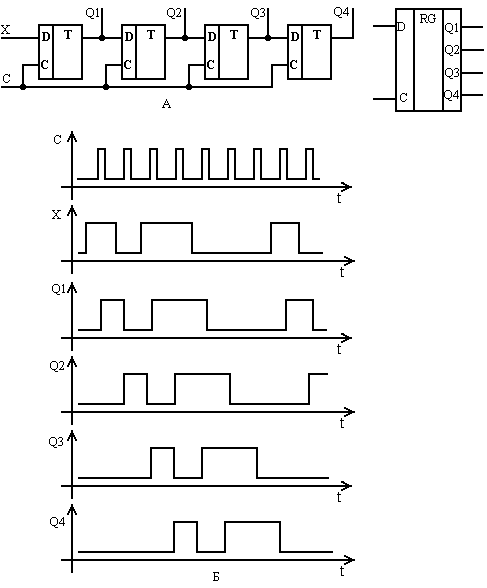
\includegraphics[width=0.6\textwidth]{14_register.png}
\caption{Регистр: схема реализации, УГО, схема сигналов}
\label{fig:14_register}
\end{figure}

\subsection*{Классификация регистров}

\begin{itemize}
\item накопительные;
\item сдвигающие. Которые в свою очередь делятся на:
	\begin{itemize}
	\item по способу ввода-вывода информации:
		\begin{itemize}
		\item параллельные
			\par запись и считывание информации происходит одновременно на все входы и со всех выходов
		\item последовательные
			\par запись и считывание информации происходит в первый триггер, а та информация, которая была в этом триггере, перезаписывается в следующий - то же самое происходит и с остальными триггерами
		\item комбинированные
		\end{itemize}
	\item по направлению передачи информации:
		\begin{itemize}
			\item однонаправленные
			\item реверсивные
		\end{itemize}
	\item по основанию системы счисления:
		\begin{itemize}
			\item двоичные
			\item троичные
			\item десятичные
		\end{itemize}
	\end{itemize}
\end{itemize}

Счётчик числа импульсов — устройство, на выходах которого получается двоичный (двоично-десятичный) код, определяемый числом поступивших импульсов. Счётчики могут строиться на двухступенчатых D-триггерах, T-триггерах и JK-триггерах.

Основной параметр счётчика — модуль счёта — максимальное число единичных сигналов, которое может быть сосчитано счётчиком. Счётчики обозначают через СТ (от англ. counter).

\subsection*{Классификация счетчиков}

\begin{itemize}
\item по числу устойчивых состояний триггеров
	\begin{itemize}
	\item на двоичных триггерах
	\item на троичных триггерах
	\item на n-ичных триггерах
	\end{itemize}
\item по модулю счёта:
	\begin{itemize}
	\item двоично-десятичные (декада)
	\item двоичные
	\item с произвольным постоянным модулем счёта
	\item с переменным модулем счёта
	\end{itemize}
\item по направлению счёта:
	\begin{itemize}
	\item суммирующие
	\item вычитающие
	\item реверсивные
	\end{itemize}
\item по способу формирования внутренних связей:
	\begin{itemize}
	\item с последовательным переносом
	\item с ускоренным переносом
		\begin{itemize}
		\item с параллельным ускоренным переносом
		\item со сквозным ускоренным переносом
		\end{itemize}
	\item с комбинированным переносом
	\item кольцевые
	\end{itemize}
\item по способу переключения триггера:
	\begin{itemize}
	\item синхронные
	\item асинхронные
	\end{itemize}
\item Счётчик Джонсона
	\par Счетчиком Джонсона называют кольцевой регистр, который строится на основе замкнутого регистра сдвига с одной перекрестной инверсной связью. Счетчик имеет коэффициент пересчета, вдвое больший числа составляющих его триггеров.
\end{itemize}


% Вопрос 15 ---------------------------------------------------------------------------------------------------------------
\section{Цифро-аналоговые преобразователи. Назначение. Принцип работы. Матрица R-2R. Область применения.}

Цифро-аналоговый преобразователь (ЦАП) — устройство для преобразования цифрового (обычно двоичного) кода в аналоговый сигнал (ток, напряжение или заряд). Цифро-аналоговые преобразователи являются интерфейсом между дискретным цифровым миром и аналоговыми сигналами.

Наиболее общие типы электронных ЦАП:

\begin{itemize}
\item Широтно-импульсный модулятор — простейший тип ЦАП. Стабильный источник тока или напряжения периодически включается на время, пропорциональное преобразуемому цифровому коду, далее полученная импульсная последовательность фильтруется аналоговым фильтром нижних частот. Такой способ часто используется для управления скоростью электромоторов, а также становится популярным в Hi-Fi-аудиотехнике;

\item ЦАП передискретизации, такие как дельта-сигма-ЦАП, основаны на изменяемой плотности импульсов. Передискретизация позволяет использовать ЦАП с меньшей разрядностью для достижения большей разрядности итогового преобразования; часто дельта-сигма ЦАП строится на основе простейшего однобитного ЦАП, который является практически линейным. На ЦАП малой разрядности поступает импульсный сигнал с модулированной плотностью импульсов (c постоянной длительностью импульса, но с изменяемой скважностью), создаваемый с использованием отрицательной обратной связи. Отрицательная обратная связь выступает в роли фильтра верхних частот для шума квантования.

\item Большинство ЦАП большой разрядности (более 16 бит) построены на этом принципе вследствие его высокой линейности и низкой стоимости. Быстродействие дельта-сигма ЦАП достигает сотни тысяч отсчетов в секунду, разрядность — до 24 бит. Для генерации сигнала с модулированной плотностью импульсов может быть использован простой дельта-сигма модулятор первого порядка или более высокого порядка как MASH (англ. Multi stage noise SHaping). С увеличением частоты передискретизации смягчаются требования, предъявляемые к выходному фильтру низких частот и улучшается подавление шума квантования;

\item ЦАП взвешивающего типа, в котором каждому биту преобразуемого двоичного кода соответствует резистор или источник тока, подключенный на общую точку суммирования. Сила тока источника (проводимость резистора) пропорциональна весу бита, которому он соответствует. Таким образом, все ненулевые биты кода суммируются с весом. Взвешивающий метод один из самых быстрых, но ему свойственна низкая точность из-за необходимости наличия набора множества различных прецизионных источников или резисторов и непостоянного импеданса. По этой причине взвешивающие ЦАП имеют разрядность не более восьми бит;

\item ЦАП лестничного типа (цепная R-2R-схема). В R-2R-ЦАП значения создаются в специальной схеме, состоящей из резисторов с сопротивлениями R и 2R, называемой матрицей постоянного импеданса, которая имеет два вида включения: прямое — матрица токов и инверсное — матрица напряжений. Применение одинаковых резисторов позволяет существенно улучшить точность по сравнению с обычным взвешивающим ЦАП, так как сравнительно просто изготовить набор прецизионных элементов с одинаковыми параметрами. ЦАП типа R-2R позволяют отодвинуть ограничения по разрядности. С лазерной подгонкой резисторов на одной подложке достигается точность 20-22 бита. Основное время на преобразование тратится в операционном усилителе, поэтому он должен иметь максимальное быстродействие. Быстродействие ЦАП единицы микросекунд и ниже (то есть наносекунды);
\end{itemize}

ЦАП находятся в начале аналогового тракта любой системы, поэтому параметры ЦАП во многом определяют параметры всей системы в целом. Далее перечислены наиболее важные характеристики ЦАП.

\begin{itemize}
\item Разрядность — количество различных уровней выходного сигнала, которые ЦАП может воспроизвести. Обычно задается в битах; количество бит есть логарифм по основанию 2 от количества уровней. Например, однобитный ЦАП способен воспроизвести два ($2^1$) уровня, а восьмибитный — 256 ($2^8$) уровней. Разрядность тесно связана с эффективной разрядностью (англ. ENOB, Effective Number of Bits), которая показывает реальное разрешение, достижимое на данном ЦАП.

\item Максимальная частота дискретизации — максимальная частота, на которой ЦАП может работать, выдавая на выходе корректный результат. В соответствии с теоремой Найквиста — Шеннона (известной также как теорема Котельникова), для корректного воспроизведения аналогового сигнала из цифровой формы необходимо, чтобы частота дискретизации была не менее, чем удвоенная максимальная частота в спектре сигнала. Например, для воспроизведения всего слышимого человеком звукового диапазона частот, спектр которого простирается до 20 кГц, необходимо, чтобы звуковой сигнал был дискретизован с частотой не менее 40 кГц. Стандарт Audio CD устанавливает частоту дискретизации звукового сигнала 44,1 кГц; для воспроизведения данного сигнала понадобится ЦАП, способный работать на этой частоте. В дешевых компьютерных звуковых картах частота дискретизации составляет 48 кГц. Сигналы, дискретизованные на других частотах, подвергаются передискретизации до 48 кГц, что частично ухудшает качество сигнала.

\item Монотонность — свойство ЦАП увеличивать аналоговый выходной сигнал при увеличении входного кода.

\item THD+N (суммарные гармонические искажения + шум) — мера искажений и шума вносимых в сигнал ЦАПом. Выражается в процентах мощности гармоник и шума в выходном сигнале. Важный параметр при малосигнальных применениях ЦАП.

\item Динамический диапазон — соотношение наибольшего и наименьшего сигналов, которые может воспроизвести ЦАП, выражается в децибелах. Данный параметр связан с разрядностью и шумовым порогом.

\item Статические характеристики:
	\begin{itemize}
	\item DNL (дифференциальная нелинейность) — характеризует, насколько приращение аналогового сигнала, полученное при увеличении кода на 1 младший значащий разряд (МЗР), отличается от правильного значения;
	\item INL (интегральная нелинейность) — характеризует, насколько передаточная характеристика ЦАП отличается от идеальной. Идеальная характеристика строго линейна; INL показывает, насколько напряжение на выходе ЦАП при заданном коде отстоит от линейной характеристики; выражается в МЗР;
	\item усиление;
	\item смещение.
	\end{itemize}

\item Частотные характеристики:
	\begin{itemize}
	\item SNDR (отношение сигнал/шум+искажения) — характеризует в децибелах отношение мощности выходного сигнала к суммарной мощности шума и гармонических искажений;
	\item HDi (коэффициент i-й гармоники) — характеризует отношение i-й гармоники к основной гармонике;
	\item THD (коэффициент гармонических искажений) — отношение суммарной мощности всех гармоник (кроме первой) к мощности первой гармоники.
	\end{itemize}
\end{itemize}

\begin{figure}[H]
\centering
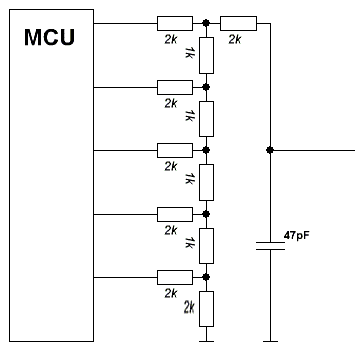
\includegraphics[width=0.5\textwidth]{15_R2R.png}
\caption{Схема R2R-матрицы}
\label{fig:15_R2R}
\end{figure}


% Вопрос 16 ---------------------------------------------------------------------------------------------------------------
\section{Аналого-цифровые преобразователи. Классификация. Область применения. Параллельные АЦП. АЦП поразрядного взвешивания.}

Аналого-цифровой преобразователь (АЦП, англ. Analog-to-digital converter, ADC) — устройство, преобразующее входной аналоговый сигнал в дискретный код (цифровой сигнал). Обратное преобразование осуществляется при помощи ЦАП (цифро-аналогового преобразователя, DAC).

Как правило, АЦП — электронное устройство, преобразующее напряжение в двоичный цифровой код. Тем не менее, некоторые неэлектронные устройства с цифровым выходом, следует также относить к АЦП, например, некоторые типы преобразователей угол-код. Простейшим одноразрядным двоичным АЦП является компаратор.

\begin{figure}[H]
\centering
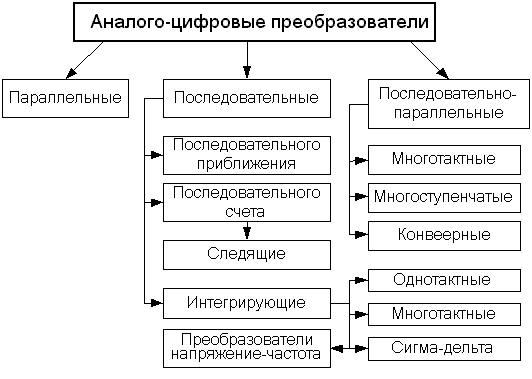
\includegraphics[width=0.7\textwidth]{16_ADC_scheme.png}
\caption{Классификация АЦП}
\label{fig:16_ADC_scheme}
\end{figure}

\subsection*{АЦП параллельного типа}
АЦП параллельного типа осуществляют квантование сигнала одновременно с помощью набора компараторов, включенных параллельно источнику входного сигнала. Ниже показана реализация параллельного метода АЦ-преобразования для 3-разрядного числа.

\begin{figure}[H]
\centering
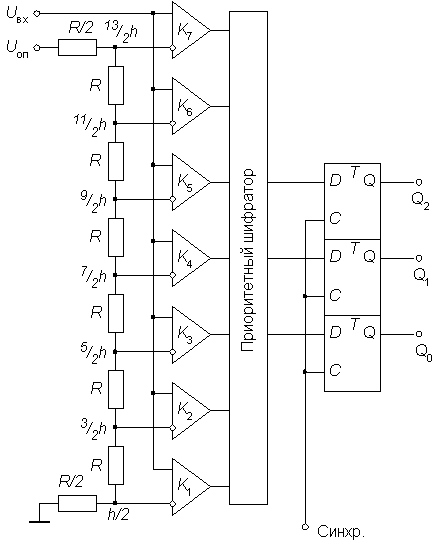
\includegraphics[width=0.6\textwidth]{16_parallel_ADC.png}
\caption{Устройство параллельного АЦП}
\label{fig:16_parallel_ADC}
\end{figure}

С помощью трех двоичных разрядов можно представить восемь различных чисел, включая нуль. Необходимо, следовательно, семь компараторов. Семь соответствующих эквидистантных опорных напряжений образуются с помощью резистивного делителя.

Параллельный АЦП является не только самым простым преобразователем с точки зрения операционной, но также и самым быстрым из всех типов АЦП, причём скорость работы ограничивается лишь задержкой на прохождение сигнала на логическом элементе и компараторе. К сожалению, в состав параллельных АЦП входит большое количество компонентов, причём размер схемы тем больше, чем выше разрядность АЦП. Для трёхразрядного АЦП требуются семь компараторов. В четырёхразрядной модели используется уже пятнадцать компараторов. По мере увеличения разрядности на одну единицу количество требуемых компараторов удваивается. Принимая в расчёт то, что восемь разрядов обычно считаются минимальным числом для обеспечения достаточной точности АЦП (то есть в случае параллельного АЦП необходимо 255 компараторов!), выявляется основная слабость технологии параллельных АЦП.

Другим, обычно не учитываемым, достоинством параллельных АЦП является возможность работы в нелинейном режиме. В случае использования в цепи делителя напряжения резисторов с равным номиналом каждый следующий импульс двоичного кода будет представлять одно и то же приращение аналогового сигнала, что будет обеспечивать пропорциональный выход. Однако в особых случаях в цепи делителя могут применяться резисторы с различными номиналами. Так образом реализуется нелинейный отклик на аналоговый входной сигнал. Никакой иной тип АЦП не позволяет обеспечить подобное преобразование сигнала путём простого изменением номиналов нескольких компонентов.

\subsection*{АЦП с поразрядным уравновешиванием}

АЦП с поразрядным уравновешиванием, является наиболее распространенным вариантом последовательных АЦП.

В основе работы этого класса преобразователей лежит принцип дихотомии, т.е последовательного сравнения измеряемой величины с 1/2, 1/4, 1/8 и т.д. от возможного максимального значения ее. Это позволяет для N-разрядного АЦП последовательного приближения выполнить весь процесс преобразования за N последовательных шагов (итераций) вместо $2^{N-1}$ при использовании последовательного счета и получить существенный выигрыш в быстродействии. Так, уже при N=10 этот выигрыш достигает 100 раз и позволяет получить с помощью таких АЦП до $10^5$...$10^6$ преобразований в секунду. В то же время статическая погрешность этого типа преобразователей, определяемая в основном используемым в нем ЦАП, может быть очень малой, что позволяет реализовать разрешающую способность до 18 двоичных разрядов при частоте выборок до 200 кГц (например, DSP101 фирмы Burr-Brown).

\begin{figure}[H]
\centering
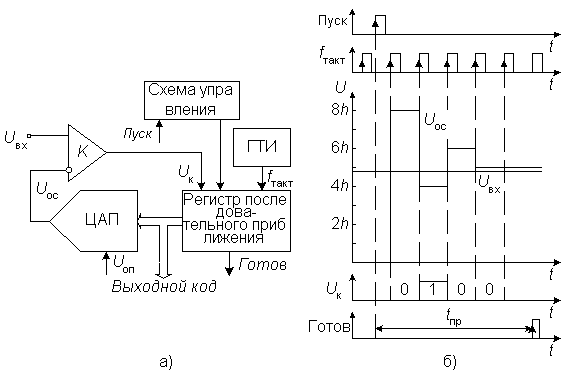
\includegraphics[width=0.8\textwidth]{16_ADC_serial_approx.png}
\caption{а) Устройство АЦП поразрядного взвешивания; б) Временная диаграмма}
\label{fig:16_ADC_serial_approx}
\end{figure}


% Вопрос 17 ---------------------------------------------------------------------------------------------------------------
\section{Интегрирующие АЦП. АЦП двойного интегрирования.}

\subsection*{Общие особенности}

АЦП данного типа осуществляют преобразование в два этапа.

\begin{enumerate}
\item На первом этапе входной аналоговый сигнал интегрируется и это проинтегрированное значение преобразуется в импульсную последовательность. Частота следования импульсов в этой последовательности или их длительность бывает промодулирована проинтегрированным значением входного сигнала.
\item На втором этапе эта последовательность импульсов преобразуется в цифровой код - измеряется ее частота или длительность импульсов.
\end{enumerate}

\subsection*{Общие достоинства}

\begin{enumerate}
\item АЦП данного типа нечувствительны к импульсным помехам.
\item АЦП данного типа нечувствительны к периодическим помехам если их период в целое число раз меньше периода интегрирования.
\item В результате, АЦП данного типа являются наиболее точными - типичная точность - 4...6 десятичных знаков, что соответствует 14...20 двоичным разрядам.
\item При работе АЦП данного типа в составе микропроцессорной системы возможна программная реализация части измерительной процедуры, а именно второго этапа - измерения временных характеристик последовательности импульсов, что упрощает преобразователь.
\end{enumerate}

\subsection*{Общие недостатки}

Преобразователи данного типа являются наименее быстродействующими из всех - типичное время преобразования - 1 - 1000 мс.

\subsection*{Программная реализация части преобразовательной процедуры}

Как уже отмечалось, при работе АЦП данного типа в составе микропроцессорной системы возможна программная реализация части измерительной процедуры, а именно второго этапа - измерения временных характеристик последовательности импульсов. Это измерение возможно как чисто программно при отсчете времени по счетчику команд или циклов, так и с использованием таймеров. В частности, для данных целей очень хорошо подходит устройство PCA, входящее в состав расширенных вариантов микроконтроллеров семейства MCS-51.

\subsection*{Классификация и примеры построения}

АЦП данного типа классифицируются, как правило, по типу преобразователя напряжение - импульная последовательность. Бывают преобразователи напряжение-частота (ПНЧ) либо - напряжение-время (ПНВ). Кроме того возможно построение преобразователей с постоянным тактом, циклом, зарядом или напряжением. Рассмотрим два варианта построения интегрирующих АЦП

\subsection*{АЦП с двойным интегрированием}

Это двухтактный преобразователь с заданной длительностью первого такта.

В течении первого такта происходит заряд интегрирующего конденсатора. Напряжение на нем в конце такта пропорционально интегралу входного напряжения.

Во время второго такта преобразования происходит разряд конденсатора заданным током до нулевого напряжения. Длительность этого такта и есть выходной сигнал преобразователя.

Достоинством данного варианта построения интегрирующего АЦП является не зависимость результата преобразователя от емкости интегрирующего конденсатора и пропорциональное изменение длительности второго такта при изменении длительности первого. Это позволяет снизить требования к точности тактовой частоты. В результате именно этот тип преобразователя используется в большинстве цифровых измерительных приборах.

\begin{figure}[H]
\centering
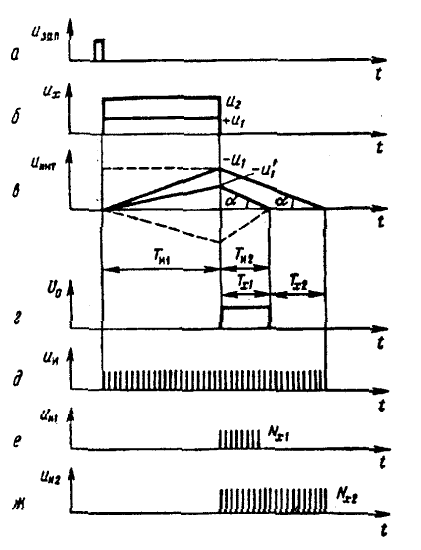
\includegraphics[width=0.5\textwidth]{17_ADC_2INT.png}
\caption{АЦП двойного интегрирования}
\label{fig:17_ADC_2INT}
\end{figure}


% Вопрос 18 ---------------------------------------------------------------------------------------------------------------
\section{Таймеры. Классификация. Область применения.}

Таймером называется устройство, предназначенное для формирования импульсных сигналов с регулируемой длительностью и скважностью. Таймеры делятся на две группы: однотактные и многотактные.

Однотактные таймеры применяются для формирования импульсов длительностью от 1 мкс до минут  и более. Многотактные таймеры включают в себя однотактный таймер и счетчик и предназначены для формирования временных интервалов длительностью в десятки часов.
Наиболее распространенным типом однотактного таймера является ИС К1006ВИ1 (NE555). Функциональная схема таймера приведена на рисунке ниже.

\begin{figure}[H]
\centering
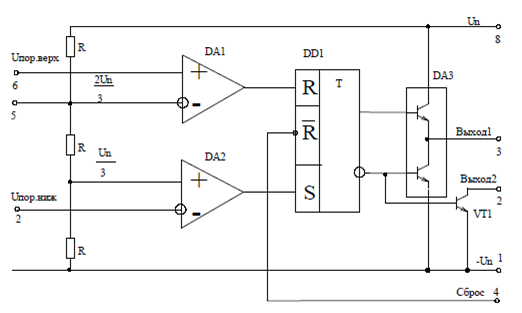
\includegraphics[width=0.7\textwidth]{18_scheme.png}
\caption{Схема таймера}
\label{fig:18_scheme_2INT}
\end{figure}

Таймер состоит из четырех функциональных устройств: двух компараторов DA1 и DA2,  RS-триггера  DD1, усилителя мощности DA3. Внутренний резистивный делитель задает пороговые напряжения, равные, 2Uп/3 для компаратора DA1 и Uп/3 для компаратора DA2. Напряжение питания Uп = 5 - 16,5в, потребляемый ток Iп = 0,7 Uп. Входные токи таймера не превышают 0,5 мкА. Максимальная частота 10 МГц. Таймер имеет второй высокоомный выход к.7.

Таймеры широко используются во многих импульсных устройствах.

На основе таймеров могут быть построены мультивибраторы, одновибраторы, преобразователи напряжения. Таймеры могут входить в состав аппаратуры систем автоматического управления. Особенностью таймеров является высокая стабильность их работы в широком интервале температур.

На рис приведена схема одновибратора, выполненная на таймере К1006ВИ1.

\begin{figure}[H]
\centering
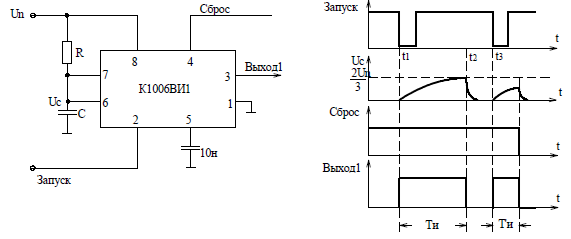
\includegraphics[width=0.7\textwidth]{18_diag.png}
\caption{Схема одновибратора на К1006ВИ1}
\label{fig:18_diag}
\end{figure}

Для работы таймера в режиме одновибратора на объединенные входы к.7 и 6 подключается цепочка RC. При поступлении на вход 2 запускающего импульса амплитудой, меньше Uп/3, триггер DD1 переворачивается, и на выходе 1 формируется прямоугольный импульс. Одновременно запирается транзистор VT1, и конденсатор С начинает заряжаться через резистор R. Напряжение Uс на входах 6,7 возрастает по экспоненте и в момент времени t2 достигает уровня 2Uп/3.

При этом срабатывает компаратор DA1, триггер DD1 возвращается в первоначальное состояние, открывается транзистор VT1, конденсатор С разряжается, и формируется задний фронт импульса на выходе 1. Длительность импульса Ти зависит от постоянной времени RC. Длительность импульса Ти = 1,1 RC.

Схема мультивибратора на базе таймера приведена на рисунке ниже.

\begin{figure}[H]
\centering
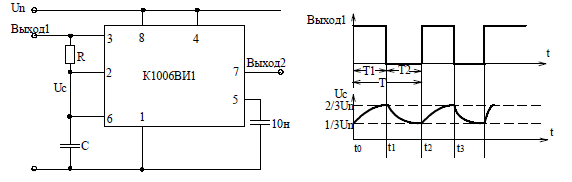
\includegraphics[width=0.7\textwidth]{18_mdiag.png}
\caption{Схема мультивибратора на базе таймера}
\label{fig:18_mdiag}
\end{figure}

Здесь входы к2 и к6 объединены и подключены на интегрирующую цепочку RC. Напряжение на емкости С UС меняется по экспоненциальному закону между уровнями Uп/3 и 2Uп/3. Период импульсов мультивибратора равен Т = 1,4 RC. Скважность равна 2.
Существует большое количество других схем, построенных на базе таймера К1006ВИ1.


% Вопрос 19 ---------------------------------------------------------------------------------------------------------------
\section{Источники вторичного напряжения. Структурные схемы. Выпрямители и фильтры.}

Вторичный источник электропитания — это устройство, предназначенное для обеспечения питания электроприбора электрической энергией, при соответствии требованиям её параметров: напряжения, тока, и т. д. путём преобразования энергии других источников питания. Согласно ГОСТ Р 52907-2008 слово «вторичный» опускается.

\subsection*{Классификация}

\begin{itemize}
\item Обеспечение передачи мощности — источник питания должен обеспечивать передачу заданной мощности с наименьшими потерями и соблюдением заданных характеристик на выходе без вреда для себя. Обычно мощность источника питания берут с некоторым запасом.
\item Преобразование формы напряжения — преобразование переменного напряжения в постоянное, и наоборот, а также преобразование частоты, формирование импульсов напряжения и т. д. Чаще всего необходимо преобразование переменного напряжения промышленной частоты в постоянное.
\item Преобразование величины напряжения — как повышение, так и понижение. Нередко необходим набор из нескольких напряжений различной величины для питания различных цепей.
\item Стабилизация — напряжение, ток и другие параметры на выходе источника питания должны лежать в определённых пределах, в зависимости от его назначения при влиянии большого количества дестабилизирующих факторов: изменения напряжения на входе, тока нагрузки и т. д. Чаще всего необходима стабилизация напряжения на нагрузке, однако иногда (например, для зарядки аккумуляторов) необходима стабилизация тока.
\item Защита — напряжение, или ток нагрузки в случае неисправности (например, короткого замыкания) каких-либо цепей может превысить допустимые пределы и вывести электроприбор, или сам источник питания из строя. Также во многих случаях требуется защита от прохождения тока по неправильному пути: например прохождения тока через землю при прикосновении человека или постороннего предмета к токоведущим частям.
\item Гальваническая развязка цепей — одна из мер защиты от протекания тока по неверному пути.
\item Регулировка — в процессе эксплуатации может потребоваться изменение каких-либо параметров для обеспечения правильной работы электроприбора.
\item Управление — может включать регулировку, включение/отключение каких-либо цепей, или источника питания в целом. Может быть как непосредственным (с помощью органов управления на корпусе устройства), так и дистанционным, а также программным (обеспечение включения/выключения, регулировка в заданное время или с наступлением каких-либо событий).
\item Контроль — отображение параметров на входе и на выходе источника питания, включения/выключения цепей, срабатывания защит. Также может быть непосредственным или дистанционным.
\end{itemize}

\subsection*{Трансформаторные ВИП}

Классическим блоком питания является трансформаторный БП. В общем случае он состоит из понижающего трансформатора или автотрансформатора, у которого первичная обмотка рассчитана на сетевое напряжение. Затем устанавливается выпрямитель, преобразующий переменное напряжение в постоянное (пульсирующее однонаправленное). В большинстве случаев выпрямитель состоит из одного диода (однополупериодный выпрямитель) или четырёх диодов, образующих диодный мост (двухполупериодный выпрямитель). Иногда используются и другие схемы, например, в выпрямителях с удвоением напряжения. После выпрямителя устанавливается фильтр, сглаживающий колебания (пульсации). Обычно он представляет собой просто конденсатор большой ёмкости.

Также в схеме могут быть установлены фильтры высокочастотных помех, всплесков (варисторы), защиты от КЗ, стабилизаторы напряжения и тока.

\begin{figure}[H]
\centering
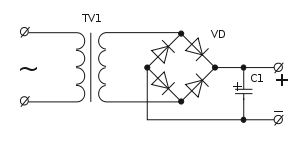
\includegraphics[width=0.8\textwidth]{19_transformer.png}
\caption{Схема простейшего трансформаторного ВИП}
\label{fig:19_transformer}
\end{figure}

\textbf{Структурная схема: трансформатор -> выпрямитель -> сглаживающий фильтр -> стабилизатор}

Достоинства трансформаторных БП:

\begin{itemize}
\item Простота конструкции.
\item Надёжность.
\item Доступность элементной базы.
\item Отсутствие создаваемых радиопомех (в отличие от импульсных, создающих помехи за счет гармонических составляющих).
\end{itemize}

Недостатки трансформаторных БП:

\begin{itemize}
\item Большой вес и габариты, пропорционально мощности.
\item Металлоёмкость.
\item Компромисс между снижением КПД и стабильностью выходного напряжения: для обеспечения стабильного напряжения требуется стабилизатор, вносящий дополнительные потери.
\item Слабая стойкость оборудования с таким БП к броскам напряжения и «отгоранию нуля» (обычно возникает в воздушных сетях сельской местности, приводит к повышению напряжения в розетках с 220 до 380 В). Печально известны в этом плане платы автоматики отопительных котлов (как правило они защищаются варистором, но часто и этого оказывается недостаточно). В то же время техника с импульсными БП (например, современные телевизоры) часто переносит повышения питания до 380 В без разрушения.
\end{itemize}

\subsection*{Импульсные ВИП}

Импульсные блоки питания являются инверторной системой. В импульсных блоках питания переменное входное напряжение сначала выпрямляется. Полученное постоянное напряжение преобразуется в прямоугольные импульсы повышенной частоты и определенной скважности, либо подаваемые на трансформатор (в случае импульсных БП с гальванической развязкой от питающей сети) или напрямую на выходной ФНЧ (в импульсных БП без гальванической развязки). В импульсных БП могут применяться малогабаритные трансформаторы — это объясняется тем, что с ростом частоты повышается эффективность работы трансформатора и уменьшаются требования к габаритам (сечению) сердечника, требуемым для передачи эквивалентной мощности. В большинстве случаев такой сердечник может быть выполнен из ферромагнитных материалов, в отличие от сердечников низкочастотных трансформаторов, для которых используется электротехническая сталь.

В импульсных блоках питания стабилизация напряжения обеспечивается посредством отрицательной обратной связи. Обратная связь позволяет поддерживать выходное напряжение на относительно постоянном уровне вне зависимости от колебаний входного напряжения и величины нагрузки. Обратную связь можно организовать разными способами. В случае импульсных источников с гальванической развязкой от питающей сети наиболее распространенными способами являются использование связи посредством одной из выходных обмоток трансформатора или при помощи оптрона. В зависимости от величины сигнала обратной связи (зависящему от выходного напряжения), изменяется скважность импульсов на выходе ШИМ-контроллера. Если развязка не требуется, то, как правило, используется простой резистивный делитель напряжения. Таким образом, блок питания поддерживает стабильное выходное напряжение.

\textbf{Структурная схема: выпрямитель -> фильтр -> генератор -> трансформатор -> выпрямитель -> фильтр -> стабилизатор}

Достоинства импульсных БП:

Сравнимые по выходной мощности с линейными стабилизаторами соответствующие им импульсные стабилизаторы обладают следующими основными достоинствами:

\begin{itemize}
\item меньшим весом за счёт того, что с повышением частоты можно использовать трансформаторы меньших размеров при той же передаваемой мощности. Масса линейных стабилизаторов складывается в основном из мощных тяжёлых низкочастотных силовых трансформаторов и мощных радиаторов силовых элементов, работающих в линейном режиме. Кроме того, благодаря повышенной частоте преобразования, значительно уменьшаются габариты фильтра выходного напряжения (можно использовать конденсаторы значительно меньшей ёмкости, чем для выпрямителей, работающих на промышленной частоте). Сам выпрямитель может быть выполнен по простейшей однополупериодной схеме, без риска увеличения пульсаций выходного напряжения;
\item значительно более высоким КПД (вплоть до 90-98 \%)[источник не указан 1182 дня] за счет того, что основные потери в импульсных стабилизаторах связаны с переходными процессами в моменты переключения ключевого элемента. Поскольку основную часть времени ключевые элементы находятся в одном из устойчивых состояний (то есть либо включен, либо выключен) потери энергии минимальны;
\item меньшей стоимостью, благодаря массовому выпуску унифицированной элементной базы и разработке ключевых транзисторов высокой мощности. Кроме этого следует отметить значительно более низкую стоимость импульсных трансформаторов при сравнимой передаваемой мощности, и возможность использования менее мощных силовых элементов, поскольку режим их работы ключевой;
\item сравнимой с линейными стабилизаторами надежностью. (Блоки питания вычислительной техники, оргтехники, бытовой электроники почти исключительно импульсные, линейные БП малой мощности сохранились только для питания слаботочных плат управления "белой"[неизвестный термин] бытовой техники вроде стиральных машин, микроволновых печей и отопительных котлов и колонок).
\item широким диапазоном питающего напряжения и частоты, недостижимым для сравнимого по цене линейного. На практике это означает возможность использования одного и того же импульсного БП для носимой цифровой электроники в разных странах мира — Россия/США/Англия, сильно отличных по напряжению и частоте в стандартных розетках.
\item наличием в большинстве современных БП встроенных цепей защиты от различных непредвиденных ситуаций, например от короткого замыкания и от отсутствия нагрузки на выходе.
\end{itemize}

Недостатки импульсных БП:

\begin{itemize}
\item Работа основной части схемы без гальванической развязки от сети, что, в частности, несколько затрудняет ремонт таких БП;
\item Все без исключения импульсные блоки питания являются источником высокочастотных помех, поскольку это связано с самим принципом их работы. Поэтому требуется предпринимать дополнительные меры помехоподавления, зачастую не позволяющие устранить помехи полностью. В связи с этим часто недопустимо применение импульсных БП для некоторых видов аппаратуры.
\item Как правило, импульсные блоки питания имеют ограничение на минимальную мощность нагрузки. Если мощность нагрузки ниже минимальной, блок питания либо не запускается, либо параметры выходных напряжений (величина, стабильность) могут не укладываться в допустимые отклонения.
\item В распределённых системах электропитания: эффект гармоник кратных трём. При наличии эффективно действующих корректоров фактора мощности и фильтров во входных цепях этот недостаток обычно не актуален.
\end{itemize}

\subsection*{Выпрямители}

Выпрямитель (электрического тока) — преобразователь электрической энергии; механическое, электровакуумное, полупроводниковое или другое устройство, предназначенное для преобразования переменного входного электрического тока в постоянный выходной электрический ток.

Большинство выпрямителей создаёт не постоянные, а пульсирующие однонаправленные напряжение и ток, для сглаживания пульсаций которых применяют фильтры.

\subsection*{Сглаживающий фильтр}

Сглаживающий фильтр — устройство для сглаживания пульсаций после выпрямления переменного тока диодным мостом. Простейшим сглаживающим фильтром является электролитический конденсатор большой ёмкости, установленный на схеме параллельно нагрузке, соблюдая полярность конденсатора. Нередко устанавливается параллельно электролитическому конденсатору плёночный (или керамический) для переменного тока ёмкостью 0,01 микрофарады, для устранения помех сети 220. Различают:

\begin{itemize}
\item Индуктивный
\item Ёмкостный
\item RC
\item LC
\end{itemize}


% Вопрос 20 ---------------------------------------------------------------------------------------------------------------
\section{Транзисторный усилительный каскад с общим эмиттером.}

Достоинства:

\begin{itemize}
\item Большой коэффициент усиления по току
\item Большой коэффициент усиления по напряжению
\item Наибольшее усиление мощности
\item Можно обойтись одним источником питания
\item Выходное переменное напряжение инвертируется относительно входного.
\end{itemize}

Недостатки:

\begin{itemize}
\item Худшие температурные и частотные свойства по сравнению со схемой с общей базой
\end{itemize}

Усилительный каскад по схеме с общим эмиттером может выполнятся как на транзисторах типа p-n-p, так и на транзисторах типа n-p-n. В качестве нагрузочного элемента каскада используется резистор Rk, включенный в коллекторную цепь транзистора, либо дополнительный нагрузочный элемент Rн, включаемый параллельно выходам коллектора и эмиттера транзистора. В последнем случае усилительный каскад является инвертируемым.

Основными элементами схемы являются транзистор VT и резистор в цели коллектора Rk. Остальные элементы играют вспомогательную роль. Резисторы R1 и R2 создают напряжение смещения Uсм на базе транзистора и тем самым обеспечивают заданный режим работы усилителя. Конденсаторы Cg разделяют переменную и постоянную составляющие входного и выходного сигналов.

\begin{figure}[H]
\centering
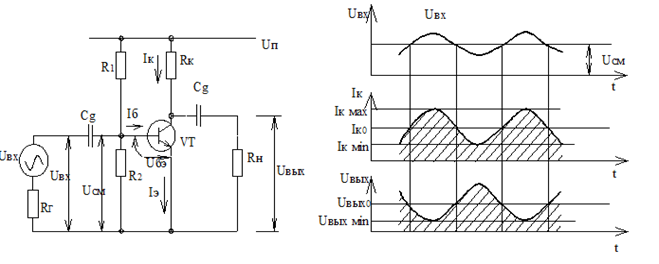
\includegraphics[width=0.8\textwidth]{20_OE.png}
\caption{Схема включения транзистора с общим эмиттером и временная диаграмма его работы}
\label{fig:20_OE}
\end{figure}

При отсутствии входного сигнала выходной ток и выходное напряжение постоянны: Ik = Ik0 и Uk = Uk0.

При поступлении на вход сигнала Uвх он усиливается в Ku раз и снимается с выхода в противофазе по отношению к входному сигналу.

Для усилителя с ОЭ Rвх = $R1 \mid\mid R2 \mid\mid$ Rвх.э ,где Rвх.э = $\beta$Rвх.б. Обычно $R1 \mid\mid R2 \geq (2 \div 5)$Rвх.э ,где Rвх.э не превышает $1 \geq 3$ кОм.

Коэффициент усиления по току $K_I = \beta \dfrac{R_K  \mid\mid R_H}{R_H}$

Таким образом, каскад с ОЭ имеет большой коэффициент усиления по току, который  при Rk>>Rн стремится к $\beta$.

Коэффициент усиления по напряжению $K_U = \beta \dfrac{R_K  \mid\mid R_H}{R_\text{Г} + R_\text{вхб}}$

Коэффициент усиления Ku возрастает с увеличением $\beta$ и $R_H$. Обычно $K_U \approx 10 \div 100$ и выше.

Коэффициент усиления по мощности Kp = Ku * Ki составляет (0,2 – 5)*$10^3$.

Выходное сопротивление каскада с ОЭ Rвых = $R_K \mid\mid r_\text{КЭ}$. Обычно $r_\text{КЭ} >> R_K$ и $R_\text{вых} \approx R_K$.

Усилительный каскад с ОЭ осуществляет поворот по фазе на 1800 выходного напряжения относительно входного.

Основные режимы работы усилителя. В зависимости от величины смещения на базе транзистора Uсм различают следующие режимы работы усилителя: A, B, AB, C, D.

\subsection*{Класс A}

Режим A характеризуется выбором рабочей точки на линейном участке входной характеристики рисунке ниже. В исходном состоянии транзистор открыт напряжением смещения Uсм и в цепи коллектора протекает ток Iко. При поступлении входного сигнала на выходе усилителя появляется выходной сигнал в противофазе по отношению ко входному.

Режим А характерен тем, что форма выходного сигнала Uвых(t) повторяет форму входного сигнала Uвх(t) за счет работы транзистора в активной зоне без захода в область насыщения и отсечки. Режим характеризуется минимальными нелинейными искажениями.
В то же время работа усилителя в режиме А характеризуется низким КПД, который теоретически не может превышать 0,5, что объясняется постоянным током Iко вне зависимости от наличия или отсутствия входного сигнала. Поэтому такой режим используется только в маломощных каскадах, в которых необходимо иметь минимальные нелинейные искажения.

\begin{figure}[H]
\centering
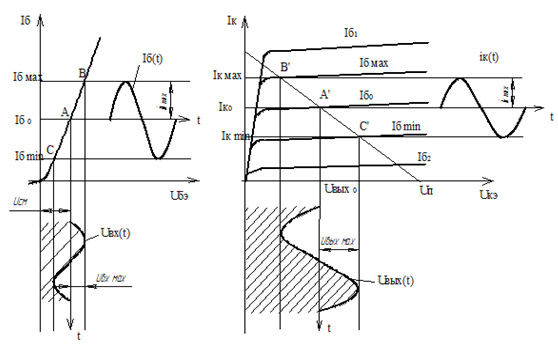
\includegraphics[width=0.6\textwidth]{20_GAA.png}
\caption{Входная и выходная характеристика при работе в классе A}
\label{fig:20_GAA}
\end{figure}

Графоаналитический метод расчета усилителя. По графикам можно определить:

Коэффициент усиления по току $K_I = \dfrac{I_{Kmax}}{I_{bmax}}$

Коэффициент усиления по напряжению $K_U = \dfrac{U_{out.max}}{U_{in.max}}$

Коэффициент усиления по мощности $K_P = K_U K_I$

\subsection*{Класс B}

Режим В характеризуется тем, что напряжение смещения Uсм=0, а следовательно, рабочая точка выбирается в самом начале входной характеристики. Особенностью режима В является то, что при отсутствии входного сигнала отсутствуют базовые и коллекторные токи. 
При поступлении входного сигнала ток в коллекторе имеет пульсирующий характер и протекает в течение половины периода. Режим В характеризуется высоким КПД, который может достигать 70\%, однако выходной сигнал сильно искажается. Поэтому такой режим применяется только в двухтактных усилителях.

\begin{figure}[H]
\centering
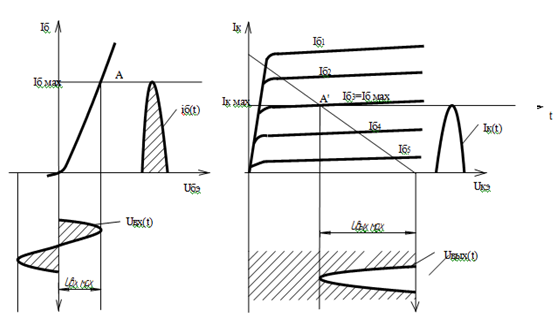
\includegraphics[width=0.6\textwidth]{20_GAB.png}
\caption{Входная и выходная характеристика при работе в классе B}
\label{fig:20_GAB}
\end{figure}

\subsection*{Класс AB}

Режим АВ занимает промежуточное положение между режимами А и В. Он характеризуется небольшим напряжением смещения Uсм и меньшими нелинейными искажениями по сравнению с режимом В. Режим АВ используется в высококачественных двухтактных усилителях мощности.

\subsection*{Класс C}

Режим С характеризуется тем, что рабочая точка на входной характеристике сдвинута влево от начала координат. Следовательно, более половины периода транзистор находится в закрытом состоянии. Режим С характеризуется высоким КПД, большими нелинейными искажениями и применяется в генераторах частоты.

\subsection*{Класс D}

Режим D характеризуется тем, что усилительный элемент может находиться в открытом  (режим насыщения) либо в закрытом (режим отсечки) состояниях. В режиме насыщения базовый ток $I_\text{Б} = \dfrac{I_K\gamma}{\beta}$, где $\gamma$ – коэффициент насыщения транзистора, который принимается равным 1,5 – 2.

Таким образом, ток в выходной цепи может принимать только два значения: Ik.max = Iнас. и I k.min $\approx$ 0. Скорость перехода из одного состояния в другое характеризует быстродействие усилительного элемента. Обычно U нас. < 1B, поэтому КПД такого усилительного каскада близок к 1.

Режим работы D, который называют еще ключевым режимом, применяется в импульсных схемах.

\begin{figure}[H]
\centering
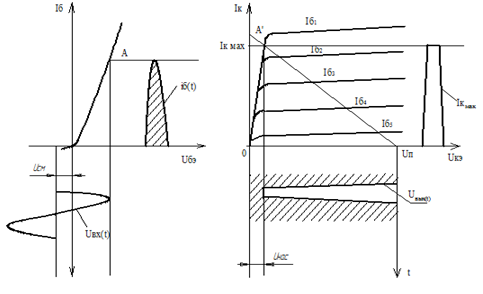
\includegraphics[width=0.6\textwidth]{20_GAD.png}
\caption{Входная и выходная характеристика при работе в классе D}
\label{fig:20_GAD}
\end{figure}


% Вопрос 21 ---------------------------------------------------------------------------------------------------------------
\section{Дискретные цифровые САР: математическое описание, Z передаточные функции.}

Дискретными принято называть такие системы, в которых некоторые сигналы, передаваемые по каналам связи замкнутой системы, существуют только в отдельный момент времени или значение этих сигналов изменяется скачкообразно, ступенчато. Поэтому существует несколько типов дискретных систем, например, в которых производится квантование по уровню или по времени. % FIXME: картинка с квантованием

В цифровых системах управления квантование производится одновременно и по уровню и по времени. Значение сигнала существует в цифровой форме, соответствующей числу уровней в дискретные моменты времени. % FIXME: картинка с квантованием

\subsection*{Математическое описание дискретных систем}

Непрерывному сигналу x(t) в дискретных системах ставится в соответствие сигнал, соответствующий дискретному моменту времени:

\begin{equation}
x(t) = x(k\tau_r) \text{, где}
\end{equation}
\par $ k = 0, 1, 2, \ldots $;\nopagebreak
\par $ \tau_r $ --- период дискретизации.

Обычно дискретная система управления строится по следующему принципу:

\begin{figure}[H]
\centering
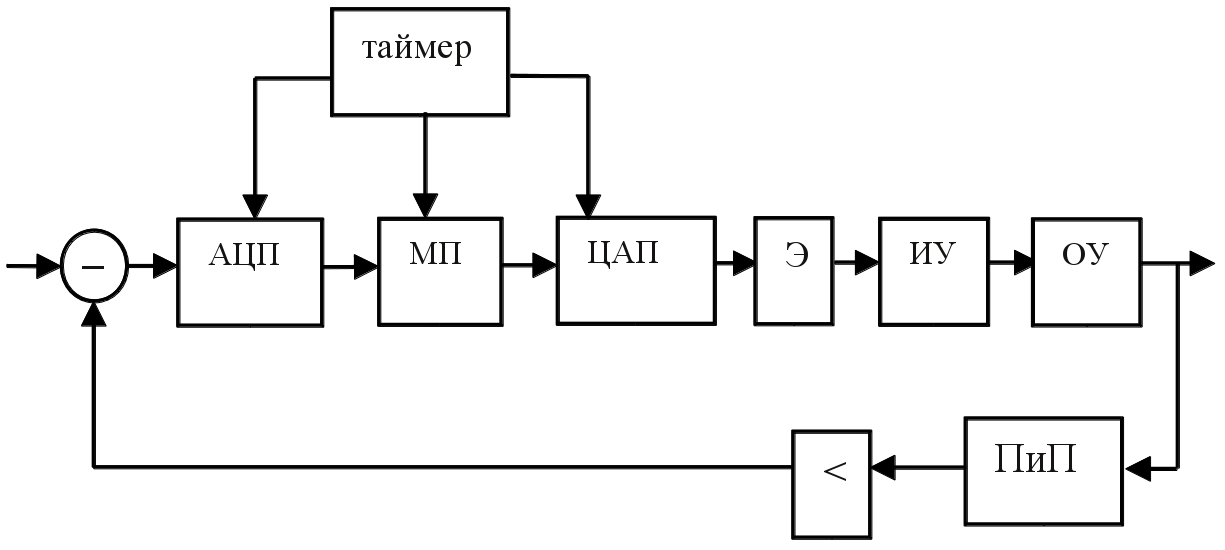
\includegraphics[width=0.7\linewidth]{21_dicret_struct.png}
\caption{Структура дискретной САУ}
\label{fig:21_dicret_struct}
\end{figure}

Это дискретная непрерывная система, в которой имеется аналоговый вход. А МП выступает в качестве цифрового регулятора. Таймер задает тактовые импульсы для процедур квантования по времени и выходных процедур. МП производит цифровую обработку сигнала в соответствии с законом регулирования. ЦАП преобразует число в последовательность импульсов, амплитуда которых может быть представлена ступенчато. Учитывая, что сигналы имеют малую мощность, то для управления эту мощность нужно усилить. Это делает экстраполятор --- заполняет промежуток между последующими импульсами по определенному закону. Простейший экстраполятор запоминает значение импульса на такт вперед. Он формирует ступенчатую огибающую последовательности импульса.

Дискретизация по времени приводит к тому, что система как замкнутая работает только в дискретные моменты времени. Поэтому упрощенная структура цифровых систем управления после линеаризации и структурных преобразований может быть представлена в виде совокупности линейной части и ключевого элемента:

\begin{figure}[H]
\centering
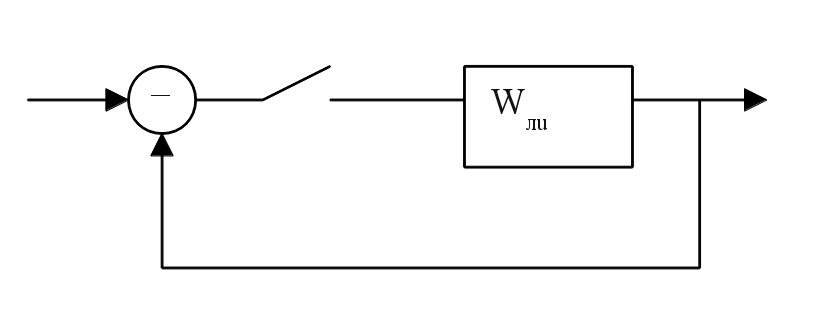
\includegraphics[width=0.5\linewidth]{21_dicret_struct_small.png}
\caption{Упрощённая структура дискретной САУ}
\label{fig:21_dicret_struct_small}
\end{figure}

Такое упрощение возможно благодаря высокому быстродействию современных вычислительных средств, то есть такая структура не учитывает запаздывания, создаваемого вычислительной процедурой.

Математическое представление дискретных систем сводится к представлению ДУ с помощью упрощенных процедур \textit{вычисления конечных разностей}.

Если в непрерывной системе вычисление первой производной представляется с помощью ДУ, то в дискретной системе $ \left( \dfrac{dx}{dt} \rightarrow \dfrac{\Delta^1x}{\tau_r} \right)  $  --- первая разность к периоду дискретизации:
\begin{equation}
\Delta^1x = x((k + 1)\tau_r) - x(k\tau_r).
\end{equation}

Для вычисления второй производной можно использовать равенство:

\begin{equation}
\left( \dfrac{d^2x}{dt^2} = \dfrac{\Delta^2x}{\tau^2_r} \right) \text{, где}
\end{equation}
\par $ \Delta^2x = \Delta^1((k + 1)\tau_r) - \Delta^1(k\tau_r) $;\nopagebreak
\par $ \Delta^2 = x((k + 1)\tau_r) - x((k + 1)\tau_r) - x((k + 1)\tau_r) + x(k\tau_r) $.

Используя процедуры численного интегрирования с использованием разностных процедур (например, на ЭВМ) можно получить следующее выражение, характеризующее дискретную САР:
\begin{equation}
y(k) = \sum_{i=0}^{m} x(k-m-i) - \sum_{j=0}^{n} y(k-n+i).
\end{equation}

Числа $y(k-n+i)$ и $x(k-m+j)$ характеризуют предыдущие значения выхода и входа ЦВМ, запоминаемые в памяти. Это уравнение называют \textit{рекурсивным или разностным}.

Реакция дискретной системы на дискретный сигнал так же может определяться с использованием принципа свертки функции:
\begin{equation}
y(k) = \sum_{k=0}^{n} x(k) w(k-n)\text{, где}
\end{equation}
\par $w(m)$ – весовая временная последовательность, аналог интеграла свертки.

Физический смысл: если на вход системы подается некий сигнал, который представлен в дискретной форме в момент времени $ k\tau $, будет соответствовать сумме реакций.

\subsection*{Z передаточные функции дискретных и цифровых САУ}

Z-преобразование получается путем замены переменных в дискретных преобразованиях Лапласа. Z-изображение дискретных сигналов дает возможность найти соотношение между z-изображением входных и выходных дискретных сигналов.

Z-преобразование содержит информацию о соответствующей непрерывной  функции времени только в дискретные моменты, поэтому оно определяет не непрерывную функцию, а ряд ее последовательных дискретных значений. Введение новой независимой переменной $ Z=e^{s\tau} $ позволяет перейти к рациональной функции:
\begin{equation}
Z[x^*\tau] = X(z) = \sum_{k=0}^{\infty} x(k\tau) Z^{-k}.
\end{equation}

Обратное Z-преобразование определяется формулой:
\begin{equation}
X^*(t) = Z^{-1} [X(z)] = \dfrac{1}{2\pi j} \oint\limits_r x(z) z^{k -1} dz
\end{equation}

Сигнал на выходе дискретных систем:
\begin{equation}
g(k) = \sum_{m=-s}^{\infty} w(k - m)g(m)\text{, где}
\end{equation}
\par $ w(k) $ --- весовая временная последовательной системы.

Отсюда:
\begin{equation}
W(z) = \dfrac{Y(z)}{G(z)}.
\end{equation}

Для непрерывной части дискретной системы Z-передаточная функция определяется на основе соотношения:
\begin{equation}
W(z) = \sum_{k=0}^{\infty} w(k\tau) z^{-k} \text{, где}
\end{equation}
\par $ w(k\tau) = [w(t)]_{t=k\tau} $;\nopagebreak
\par $ k = 1, 2, 3, \ldots $;
\par $ w(t) = L^{-1} [w(s)] $.

% Вопрос 22 ---------------------------------------------------------------------------------------------------------------
\section{Анализ дискретных САР.}

Если в Z --- передаточной функции, дискретной САР с ЭВМ в контуре управления произвести замену:
\begin{equation}
W(z) = W_\text{в}(z) z[W_\text{в} W_\text{о} W_\text{ос}].
\end{equation}

Полагая, что передаточная функция обратной связи равна 1, что всегда можно обеспечить методом структурных преобразований, передаточную функцию контура можно представить в виде:
\begin{equation}
\Phi(Z) = \dfrac{W(z)}{1 + W(z)}.
\end{equation}

Таким образом, характеристическое уравнение одноконтурной дискретной системы с единичными обратными связями будет выглядеть:
\begin{equation}
1 + W(z) = 0.
\end{equation}

Устойчивость дискретных систем будет определяться корнями этого характеристического уравнения.

Для устойчивости непрерывных систем необходимо чтобы корни располагались слева от мнимой оси. Если перенести комплексную плоскость $ s $ на комплексную плоскость $ z $, то получим линию, отображения мнимой оси. Для этого отображения можно использовать формулу замены переменных:
\begin{equation}
z = e^{\tau s}.
\end{equation}

Мнимой оси на комплексной плоскости $ s $ соответствует выражение $ s = j\omega $. На комплексной плоскости $ z $ уравнение мнимой оси: $ z = e^{i\tau\omega} = \cos\omega t + j\sin\omega t $.

\begin{figure}[H]
\centering
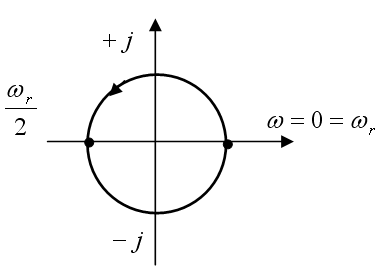
\includegraphics[width=0.4\linewidth]{22_circ.png}
$ \omega_r = \dfrac{2\pi}{\tau_r} $
\caption{Единичная окружность $ s = j\omega $}
\end{figure}

Комплексные корни $ s_i = \alpha_i + j\beta_i $ соответствуют $ z_i = e^{\alpha_i\tau_r} + e^{j\beta_i\tau_r} $. Вещественная часть корня $ \operatorname{Re} (z_i) = e^{\alpha_i\tau_r} < 1 $, следовательно левая полуплоскость $ s $ отображается во внутреннюю часть единичной окружности.

Таким образом, дискретная система устойчива, если все корни характеристического уравнения располагаются внутри единичной окружности.

% Вопрос 23 ---------------------------------------------------------------------------------------------------------------
\section{Логарифмические частотные характеристики САР.}

Решение неоднородных дифференциальных уравнений одномерной САР состоит из двух составляющих:
\begin{itemize}
\item общего решения однородного дифференциального уравнения $ X_\text{cв}(t) $, характеризующего свободное движение или переходный процесс;
\item частного решения неоднородного дифференциального уравнения $ X_\text{в}(t) $, характеризующего вынужденное движение.
\end{itemize}

Таким образом:
\begin{equation}
X_\text{вых}(t) = X_\text{св}(t) + X_\text{в}(t).
\end{equation}

\subsection*{Переходный процесс}

Интеграл уравнения $ D(s) X_\text{вых}(s) = 0 $ находится в следующем виде:
\begin{equation}
X_\text{св}(t) = C_1 e^{s_1 t} + C_2 e^{s_2 t} + \ldots + C_n e^{s_n t} \text{, где}
\end{equation}
\par $ s_i $ --- вещественные и комплексно-сопряженные корни уравнения $ D(s) = 0 $;\nopagebreak
\par $ C_1 , C_2 , \ldots, Cn $  ---  постоянные, зависящие от начальных условий.

Линейная САР, у которой переходной процесс затухает называется \textit{устойчивой}, то есть:
\begin{equation}
\lim\limits_{x \rightarrow \infty} X_\text{св}(t) = 0.
\end{equation}

При этом вещественные части корней $ s_i $ должны быть отрицательны.

\subsection*{Вынужденное движение}

Если на вход САР подается гармонический сигнал, то его можно разложить по формуле Эйлера:
\begin{equation}
f(t) = \dfrac{f_0}{2} e^{j\omega t} - \dfrac{f_0}{2} e^{-j\omega t} = f_1(t) + f_2(t).
\end{equation}

Представим $ X_\text{в}(t) = {X_\text{в}}_1(t) + {X_\text{в}}_2(t) $, тогда:
\begin{equation}
X_\text{в}(t) = f_0 A(\omega) \cos(\omega t + \varphi(\omega))\text{, где}
\end{equation}
\par $ A(\omega) $ --- амплитудно-частотная характеристика;\nopagebreak
\par $ \varphi(\omega) $  ---  фазочастотная характеристика.

\begin{figure}[H]
\centering
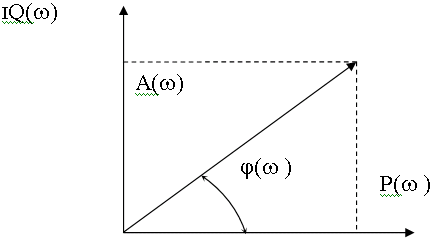
\includegraphics[width=0.5\linewidth]{23_chars.png}
\caption{Частотные характеристики САР}
\end{figure}

При анализе САР широко применяется графический метод.
\begin{enumerate}
\item При $ 0 < \omega < \omega_c $, $ A(\omega) > A(0) $ и диапазон частот от 0 до $ \omega_c $ называется  полосой пропускания, где $ \omega_c $ --- частота среза по уровню $ Aj(\omega) = 0 $ или $ Aj(\omega) = 0,707 A(0) $;
\item При $ \omega = \omega_m  $, $ A(\omega) $ принимает максимальное значение и $ \omega_m $ называемое \textit{резонансной частотой}.
\end{enumerate}

Очень удобны с практической точки зрения логарифмические частотные характеристики, которые получаются путем логарифмирования $ W(j\omega) $: $ \lg(W(j\omega)) $;

$ L(\omega) = 20\lg A(\omega) $ [дБ] называется логарифмической амплитудно-частотной характеристикой (ЛАЧХ).

\textit{Октава} --- диапазон частот между  $ \omega $ и  $ 2\omega $: $ \lg 2\omega - \lg \omega = \lg 2 $.

\textit{Декада} --- диапазон частот между $ \omega $  и  $ 10\omega $:  $ \lg 10\omega - \lg\omega = 1 $.

\begin{figure}[H]
\centering
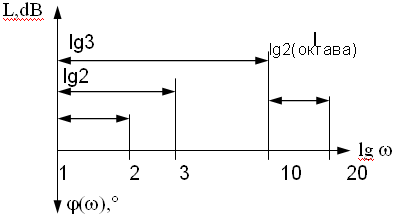
\includegraphics[width=0.5\linewidth]{23_lchars.png}
\caption{Логарифмические характеристики САР}
\end{figure}


% Вопрос 24 ---------------------------------------------------------------------------------------------------------------
\section{Переходные функции и переходные характеристики САР. Реакция САР на произвольный входной сигнал.}

Выходной сигнал САР можно определить с помощью обратного преобразования Лапласа:
\begin{equation}
X_\text{вых}(t) = \zeta^{-1}[F(s)W(s)].
\end{equation}

Если $ f(t) = \delta(-t) $ --- $ \delta $-функция, то $ F(s) = 1 $ и $ W(t) = \zeta^{-1}W(s) $ называется переходной функцией --- функцией веса.

\begin{equation}
X(t) = \dfrac{1}{2\pi j} \int\limits_{c - j\infty}^{c + j\infty} X(s) \Phi(s) e^{st} ds
\end{equation}

Если $ f(t) = l(t) $ и $ F(s) = \frac{1}{s} $, то $ h(t) = \zeta^{-1}[W(s)\frac{1}{s}] $ называют переходной функцией.

Поскольку $ W(s) $ дробно-рациональная функция, $ w(t) $  и  $ h(t) $ могут быть найдены по формулам обратного преобразования Лапласа:
\begin{equation}
X(t) = \dfrac{1}{2\pi j} \int\limits_{c - j\infty}^{c + j\infty} X(s) e^{st} dt
\end{equation}
или по теореме Хевисайда, или формуле вычетов:
\begin{equation}
X(t) = \sum_{i=1}^{n} \left[ (s - s_i)\dfrac{M(s)}{D(s)} e^{st} \right]_{s + s_i} + 2\operatorname{Re} \sum_{i=1}^{n} \left[ \dfrac{M(s)}{D'(s)} \right]_{s + s_i},
\end{equation}
где 1-ая сумма распространяется на простые вещественные корни, а 2-ая на простые комплексные.

При наличии кратных корней необходимо применять дополнительные слагаемые.

\textit{Реакция САР на произвольный входной сигнал} может быть определена с помощью интеграла свертки.

Любое производное воздействие можно представить ступенчатой линией или совокупностью дискретных значений.

\begin{figure}[H]
\centering
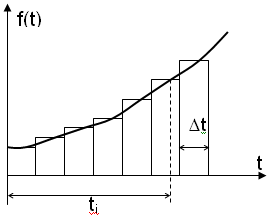
\includegraphics[width=0.45\linewidth]{24_graph.png}
\caption{Совокупность дискретных значений}
\end{figure}

\par $ t_i $  --- среднее значение времени в промежутке $ \Delta t $,\nopagebreak
\par $ f(t_i) $ --- значение функции при $ t = t_i $.



% Вопрос 25 ---------------------------------------------------------------------------------------------------------------
\section{Типовые звенья САР и их частотные и временные характеристики.}

Типовые динамические звенья:
\begin{enumerate}
\item Усилительное звено. Усиливает в $ k $ раз.
	\begin{itemize}
	\item Передаточная функция:
		\begin{equation}
		w(s) = k.
		\end{equation}
	
	\item Переходная характеристика:
		\begin{equation}
		h(t) = k.
		\end{equation}

	\item Графики ($ \uparrow : k = 1, k = 5, k = 10 $):
	
	При увеличении коэффициента усиления увеличивается амплитуда, а фаза остаётся неизменной. Таким образом, усилительное звено увеличивает амплитуду входного сигнала. Амплитуда и фаза сигнала не зависят от частоты.
	
		\begin{figure}[H]
		\centering
		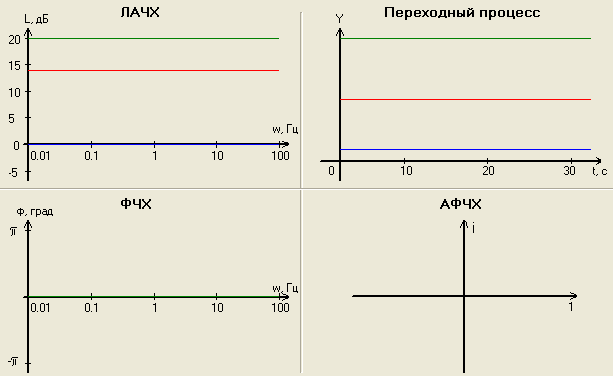
\includegraphics[width=0.7\linewidth]{25_usil.png}
		\caption{Частотные характеристики звена}
		\end{figure}
	\end{itemize}


\item Апериодическое звено первого порядка. Наклон ЛАЧХ -20 дБ/дек.
	\begin{itemize}
	\item Передаточная функция:
		\begin{equation}
		w(s) = k \dfrac{1}{Ts + 1}.
		\end{equation}
	
	\item Переходная характеристика:
		\begin{equation}
		h(t) = k(1 - e^{-\frac{t}{T}}).
		\end{equation}

	\item Графики:
	
	Чем больше постоянная времени апериодического звена $ \tau $, тем быстрее убывает амплитуда выходного сигнала при одинаковых частотах. Чем больше $ \tau $, тем медленнее (плавнее) протекает переходный процесс. Фаза стремится к $ -\pi/2 $.
	
		\begin{figure}[H]
		\centering
		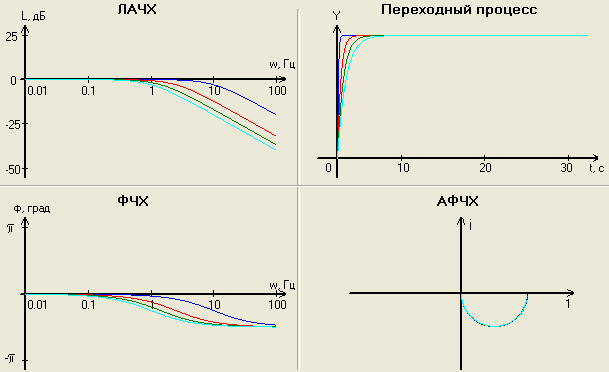
\includegraphics[width=0.75\linewidth]{25_ap1.png}
		\caption{Частотные характеристики звена}
		\end{figure}
	\end{itemize}


\item Апериодическое звено второго порядка (колебательное). Наклон ЛАЧХ -40 дБ/дек.
	\begin{itemize}
	\item Передаточная функция:
		\begin{equation}
		w(s) = k \dfrac{1}{T^2s^2 + 2\xi T s + 1}\text{, где $ \xi $ --- ошибка, \textpm{}5\% }.
		\end{equation}
	
	\item Графики:
	
	Чем больше постоянная времени колебательного звена $ \tau $, тем быстрее убывает амплитуда выходного сигнала при одинаковых частотах. Чем больше $ \tau $, тем медленнее протекает переходный процесс. Фаза стремится к $ -\pi $.
	
		\begin{figure}[H]
		\centering
		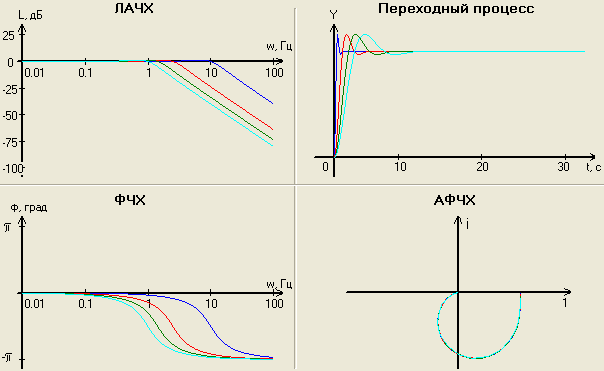
\includegraphics[width=0.75\linewidth]{25_ap2.png}
		\caption{Частотные характеристики звена}
		\end{figure}
	\end{itemize}


\item Интегрирующее звено. Наклон ЛАЧХ -20 дБ/дек.
	\begin{itemize}
	\item Передаточная функция:
		\begin{equation}
		w(s) = \dfrac{1}{s}.
		\end{equation}
	
	\item Переходная характеристика:
		\begin{equation}
		h(t) = kt.
		\end{equation}
	
	\item Графики:
	
	Амплитуда выходного сигнала зависит от частоты и с её увеличением убывает. Фаза выходного сигнала не зависит от частоты и равна $ -\pi/2 $.
	
		\begin{figure}[H]
		\centering
		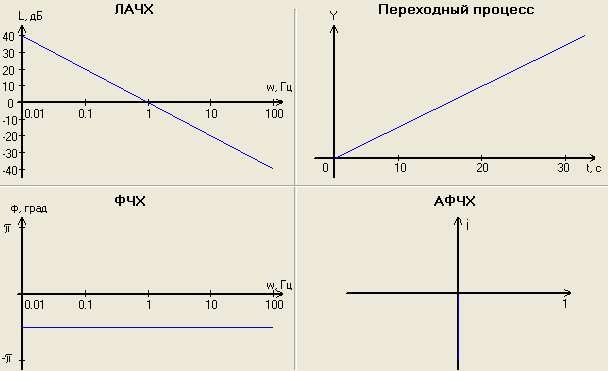
\includegraphics[width=0.75\linewidth]{25_integr.png}
		\caption{Частотные характеристики звена}
		\end{figure}
	\end{itemize}



\item Дифференцирующее звено первого порядка. Наклон ЛАЧХ 20 дБ/дек.
	\begin{itemize}
	\item Передаточная функция:
		\begin{equation}
		w(s) = Ts + 1.
		\end{equation}
	
	\item Переходная характеристика:
		\begin{equation}
		h(t) = k [\tau \delta (t) + 1(t)].
		\end{equation}
	
	\item Графики:
	
	Чем больше постоянная времени звена $ \tau $, тем быстрее возрастает амплитуда выходного сигнала при одинаковых частотах. Чем больше $ \tau $, тем медленнее протекает переходный процесс. Фаза стремится к $ \pi/2 $.
	
		\begin{figure}[H]
		\centering
		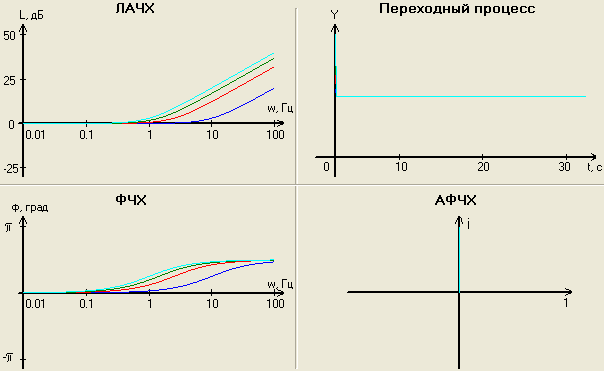
\includegraphics[width=0.75\linewidth]{25_dif1.png}
		\caption{Частотные характеристики звена}
		\end{figure}
	\end{itemize}



\item Дифференцирующее звено второго порядка. Наклон ЛАЧХ 40 дБ/дек.
	\begin{itemize}
	\item Передаточная функция:
		\begin{equation}
		w(s) = T^2s^2 + 2\xi T s + 1.
		\end{equation}
	
	\item Графики:
	
	Чем больше постоянная времени звена $ \tau $, тем быстрее возрастает амплитуда выходного сигнала при одинаковых частотах. Чем больше $ \tau $, тем медленнее протекает переходный процесс. Фаза стремится к $ \pi $;
	
		\begin{figure}[H]
		\centering
		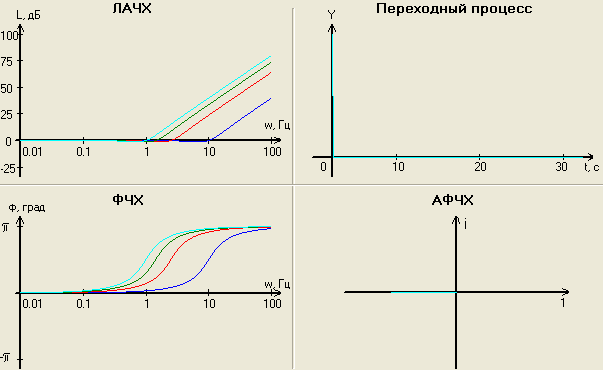
\includegraphics[width=0.75\linewidth]{25_dif2.png}
		\caption{Частотные характеристики звена}
		\end{figure}
	\end{itemize}

\end{enumerate}



% Вопрос 26 ---------------------------------------------------------------------------------------------------------------
\section{Устойчивость линейных САР: определение, теоремы Ляпунова, алгебраический критерий устойчивости Гурвица.}

Система считается \textit{устойчивой}, если отклонение выходной величины, возникшей в результате внешнего возмущения, по истечении некоторого времени становится меньше заданного.

\begin{equation}
\lim\limits_{t\rightarrow\infty} |X_\text{вых}(t)| \leq \varepsilon
\end{equation}

Таким образом, если САР выведена из состояния равновесия, а затем предоставлена самой себе, то она должна возвратится в состояние равновесия.

Ляпунов доказал 2 теоремы:
\begin{enumerate}
\item Если вещественные части всех корней характеристического уравнения 1-го приближения отрицательные, то собственное движение асимптотически устойчиво независимо от членов разложения выше 1-го порядка малости
\item Если среди корней характеристического уравнения 1-го приближения найдется по меньшей мере один с положительной вещественной частью, то собственное движение неустойчиво независимо от членов разложения выше 1-го порядка малости.
\end{enumerate}

Критические случаи имеют место, когда среди корней имеются корни с нулевой вещественной частью. Тогда вопрос об устойчивости необходимо решать исследованием полного нелинейного дифференциального уравнения.

\subsection{Алгебраический критерий устойчивости Гурвица.}

Устойчивость замкнутой динамической системы, имеющей характеристическое уравнение $ D_3(s) =  $ определяется выполнением следующих условий:
\begin{enumerate}
\item коэффициенты характеристических уравнений положительны (необходимое условие);
\item диагональные миноры больше нуля (достаточное условие).
\end{enumerate}

\begin{figure}[H]
\centering
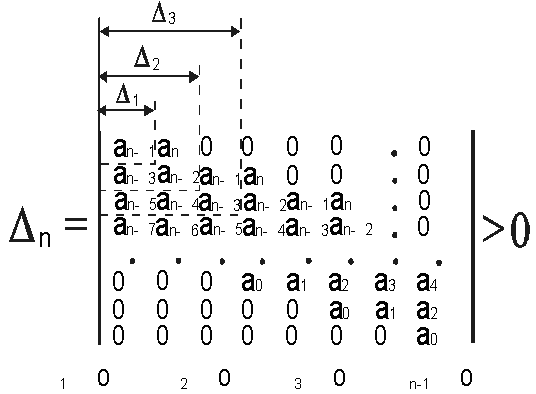
\includegraphics[width=0.5\linewidth]{26_matrix.png}
\caption{Матрица Гурвица}
\end{figure}

Определитель $ \Delta_n $ составляется следующим образом: главная диагональ состоит из коэффициентов характеристического уравнения. Начиная со второго коэффициента заполняются строки: слева --- в порядке убывания индексов, справа --- в порядке возрастания.

% Вопрос 27 ---------------------------------------------------------------------------------------------------------------
\section{Частотные критерии устойчивости линейных САР.}
% АХТУНГ: в шпорах (и соотв. тут) какая-то непонятна хуита, но более близкого варианта к тому, что требуется не найти...

\subsection*{Амплитудно-фазовый критерий устойчивости (Найквиста-Михайлова).}

Критерий получил наибольшее распространение в инженерной практике так как позволяет определить устойчивость замкнутой системы по её поведению в разомкнутом состоянии.

Характеристическое уравнение замкнутой системы может быть представлено в следующем виде:
\begin{equation}
W(s) + 1 = \dfrac{M(s) + D(s)}{D(s)} = \dfrac{D_3(s)}{D(s)} = 0.
\end{equation} % Што за бред?

Результирующий вектор:
\begin{equation}
\overline{W(j\omega) + 1} = \overline{W(j\omega)} + \overline{1}.
\end{equation}

\begin{figure}[H]
\centering
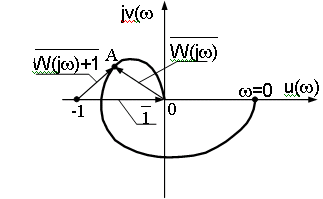
\includegraphics[width=0.3\linewidth]{27_mih_nike.png}
\caption{АФХ разомкнутой системы}
\end{figure}

\subsection*{Критерий  D-разбиения}

Метод позволяет построением одной кривой выявить сразу все значения интересующего параметра, при котором САР остается устойчивой.

Параметры САР могут быть разбиты на 3 группы:
\begin{enumerate}
\item заданные, которые обеспечиваются конструкцией системы;
\item конструктивные, которые могут быть изменены в определенных пределах;
\item настроечные.
\end{enumerate}

\subsection*{D-разбиение по одному параметру}

Характеристическое уравнение $ a_n s^n + a_{n-1} s^{n-1} + \ldots + a_1 s + a_0 = 0 $ всегда может быть представлено в следующем виде $ \mu S(s) + V(s) = 0 $, где $ \mu $ --- искомый параметр:
\begin{equation}
\mu = \dfrac{N(s)}{S(s)} = -\dfrac{N(j\omega)}{S(j\omega)} = A(\omega) = -jB(\omega).
\end{equation}

Задаваясь $ \omega $ от $ -\infty $ до $ +\infty $, строят на комплексной плоскости кривую $ D $-разбиения $ S = j\omega $. При движении от $ -\infty $ до $ +\infty $ область корней с отрицательными вещественными частями остается слева, левую сторону кривой заштриховывают.

Поскольку $ \mu $ --- действительные параметры САР, рассматриваются только точки действительной оси $ A(\omega) $, расположенные по левую сторону $ D $-кривой. Выбранные значения $ \mu $ проверяем по какому-либо критерию устойчивости.


% Вопрос 28 ---------------------------------------------------------------------------------------------------------------
\section{Анализ качества линейных САР.}

Задача анализа качества процесса регулирования заключается в нахождении ряда показателей, характеризующих переходную характеристику системы и названных первичными показателями качества.

Методы анализа качества:
\begin{itemize}
\item Частотный. Основан на рассмотренном преобразовании Лапласа $ X_\text{вых}(s) $ при $ s = j\omega $, а также на связи между частотными характеристиками замкнутых (разомкнутых) систем и переходными характеристиками.
\item Корневого годографа. Метод не требует определения корней характеристического уравнения, является графоаналитическим.
\item Логарифмического корневого годографа.
\item Интегральных оценок.
\item Косвенный. Основан на вычислении определенных интегралов по времени. Эффективен при использовании ЭВМ.
\end{itemize}

\subsection*{Частотный метод}

\begin{wrapfigure}{o}{0.45\textwidth}
\centering
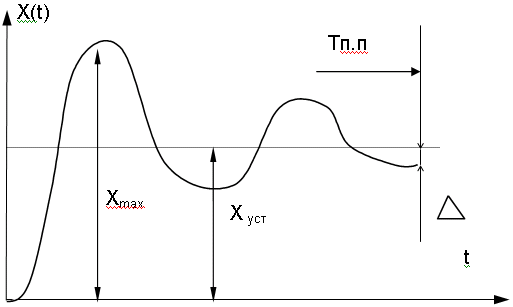
\includegraphics[width=\linewidth]{28_proc.png}
\caption{Переходный процесс}
\end{wrapfigure}

На рисунке представлены показатели характеризующие устойчивость системы.

\begin{enumerate}
\item Установившееся значение $ X_\text{уст} = X(\infty) $ определяет статическую точность системы.\\ $ E_\text{уст} = X_\text{вх} - X_\text{уст} $
\item Время перехода процесса $ T_\text{п.п.} $ определяется как наименьшее значение интервала времени, в течение которого $ [X(t)- X_\text{уст}] \leq \Delta $, где $ \Delta $ заданная постоянная малая величина (обычно$  \Delta = 0,05 X_\text{уст} $).
\item Положительное перерегулирование\\ $ \sigma = \dfrac{X_\text{max} - X_\text{уст}}{X_\text{уст}} \cdot 100\% $.
\item Число колебаний $ N $ величины $ X(t) $ в течение времени $ T_\text{п.п.} $.
\end{enumerate}

\subsection*{Определение переходных процессов}

\begin{enumerate}
\item Аналитический метод.

Если $ P_\text{З}(\omega) $ и $ Q_\text{З}(\omega) $ заданы аналитически, то удобно $ h(t) $ определять численными методами с использованием ЭВМ. Удобно использовать метод Филона интегрирования осциллирующих функций $ f(\omega) = \sin\omega t $.


\item Графоаналитический метод (метод трапецеидальных частотных характеристик).

Для построения $ P_\text{З}(\omega) $ и $ Q_\text{З}(\omega) $ применяются номограммы. Кривая $ P(\omega) $ может быть представлена в виде совокупности из некоторого числа трапецеидальных частотных характеристик:
\begin{equation}
P(\omega) \approx \sum_{i=1}^{n} r_i(\omega).
\end{equation}

Этой сумме соответствует $ h(t) $, являющееся линейной комбинацией функции $ h_i(t) $:
\begin{equation}
h(t) = \sum_{i=1}^{n} h_i(t).
\end{equation}

$ h_i(t) $ определяется по типовой вещественной частотной характеристике.
\end{enumerate}


% Вопрос 29 ---------------------------------------------------------------------------------------------------------------
\section{Синтез корректирующих устройств линейных САР.}

В автоматике применяют следующие способы коррекции динамических характеристик:
\begin{enumerate}
\item Последовательная коррекция (последовательно в прямой цепи).
\item Параллельная коррекция (параллельно прямой цепи).
\item С помощью корректирующей обратной связи (КОС).
\item Комбинированная.
\end{enumerate}

Корректирующие обратные связи уменьшают зависимость динамических свойств от изменения параметров элементов, уменьшают влияние помех но имеют высокую стоимость и громоздкость (тахогенераторы, вращающие трансформаторы).

Проектирование САР сводится к следующим этапам:
\begin{enumerate}
\item проектирование не скорректированной САР из условий физической осуществимости;
\item проектирование идеальной модели системы (желаемая характеристика);
\item компенсирование различий этих систем с помощью корректирующих цепей.
\end{enumerate}

Синтез корректирующей цепи заключается в выборе ее вида, определении передаточной функции, расчете параметров цепи.

\subsection*{Построение желаемой ЛАХ}

Порядок определения желаемой ЛАХ:
\begin{enumerate}
\item Низкочастотная асимптота проходит под наклоном $ -20\nu $ дБ/дек, где $ \nu $ --- порядок астатизма, а при частоте имеет ординату $ 20\lg k $ (дБ).
\item По заданному значению $ \sigma_\text{max} = f(P_\text{max}) $ определяет значение $ P_\text{max} $.
\par Значение $ [P_\text{min}) \approx P_\text{max} - 1 $.

\item Определяют частоту среза $ \omega_\text{ср. Tmax.} < \omega_\text{ср} < \omega_\text{ср. опт.} $, где $ \omega_\text{ср. опт.} = \sqrt{\dfrac{\omega_\text{max}}{g_0}} $.
\par $ \omega_\text{ср. опт.} $ --- заданное максимальное ускорение объекта регулирования.
\par $ \omega_\text{ср. Tmax.} $ находят по кривой $ T_\text{max} = f_1(T_\text{max}) $ при значении $ P_\text{max} $ из п.2.

\item Через точку $ \omega_\text{ср.} $  проводят среднечастотную асимптоту с наклоном -20 дБ/дек.
\item Производят сопряжение среднечастотной асимптоты с низкочастотной:
	\begin{enumerate}
	\item если в ТЗ задана точность и порядок астатизма, то $ \omega_1 \approx 0,15\omega_\text{n} $.
	\item если требования точности не определены, то сопряжение начинают с $ L_2\omega $ = +16 дБ.
	\end{enumerate}

\item Проверяют запасы устойчивости по модулю и фазе.
\item Строят высокочастотную асимптоту так, чтобы она мало отличалась от нескорректированной САР, желательно $ L_3 \approx -L_2 $.

\begin{figure}[H]
\centering
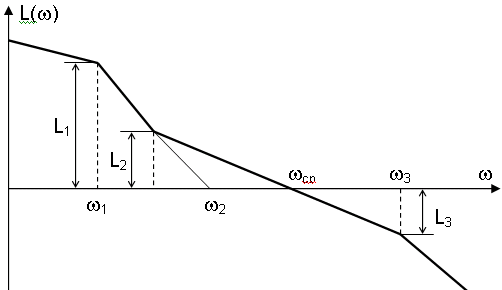
\includegraphics[width=0.5\linewidth]{29_lachh.png}
\caption{Желаемая ЛАЧХ}
\end{figure}

\end{enumerate}

\textit{Синтез КОС} может осуществляться отрицательной жесткой ОС или гибкой ОС(связью по производным).

Жесткие ООС уменьшают статический коэффициент усиления охватываемых участков, увеличивают устойчивость и ошибки в установившемся состоянии.

Охват инерционных звеньев жёсткой обратной связи (ЖОС) приводит к снижению инерционности.

Гибкие ОС (связи по производным) не оказывает влияние на статический коэффициент усиления охватываемых участков и эффективно воздействуют на форму переходных процессов и устойчивость.

Для определения $ Z(s) $ применяются следующие способы: 
\begin{enumerate}
\item эквивалентной последовательной коррекции.
\par Из условия эквивалентности
$ W_\text{пос} W_\text{охв} W_\text{неохв}  = \dfrac{W_\text{неохв} W_\text{охв}}{1 + W_\text{охв} Z} $, поэтому 
$ Z = \dfrac{1 - W_\text{пос}}{W_\text{охв} W_\text{пос}} $.
\par При таком подходе может получится физически не реализуемая передаточная функция.
\item В заданном интервале частот $ [\omega_1, \omega_2] $ обеспечивают $ ( W_\text{охв} Z ) >> 1 $, тогда  и для выполнения условия  $ (W_\text{охв} Z)  >> 1 $ вводят последовательное усилительное звено $ W(j\omega) = \dfrac{W_\text{неохв}(j\omega)}{Z(j\omega)} $.
\end{enumerate}


% Вопрос 30 ---------------------------------------------------------------------------------------------------------------
\section{Анализ нелинейных САР.}

Для анализа нелинейных систем применяются методы: фазовых траекторий, припасовывания, гармонической линеаризации, фазовой границы устойчивости и др.

\subsection*{Метод фазовых траекторий}

Фазовой плоскостью называется плоскость на которой по двум координатам X и Y откладываются какие-либо две переменные, характеризующие динамику САР, например отклонение регулируемой величины $ X $ и скорость $ X = Y = dx/dt $.

Уравнение второго порядка удобно свести к системе двух уравнений первого порядка:
\begin{equation}
\dfrac{dx}{dt} = f_1(x, y) \quad \dfrac{dy}{dt} = f_2(x, y).
\end{equation}

Для изображения на фазовой плоскости исключается время t, для чего второе делят на первое:
\begin{equation}
\dfrac{dx}{dy} = \dfrac{f_1(x, y)}{f_2(x, y)}.
\end{equation}

Получаем нелинейное дифференциальное уравнение, решение которого $ Y = F(x) $ называется \textit{фазовой траекторией}.

Для САР, линейная часть которой имеет порядок > 2, применяются \textit{многолистные фазовые плоскости}.

\subsection*{Изображения процессов регулирования на фазовой плоскости.}

\begin{enumerate}
\item Периодический незатухающий колебательный процесс.

\begin{eqnarray}
x(t) = a \sin(\omega t)			&\quad& \sin^2(\omega t) = x^2 / a^2 ;\\
y(t) = a\omega \cos (\omega t)	&\quad& \cos^2(\omega t) = y^2 / a^2 \omega^2;
\end{eqnarray}

\begin{equation}
\dfrac{x^2}{a^2} + \dfrac{y^2}{a^2 \omega^2} = 1.
\end{equation}

\begin{figure}[H]
\centering
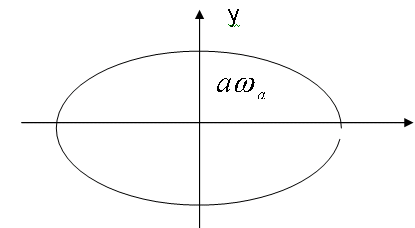
\includegraphics[width=0.4\linewidth]{30_per_nez.png}
\caption{Периодический колебательный процесс}
\end{figure}


\item Затухающий колебательный процесс.

\begin{equation}
x(t) = ae^{-nt} \cos \omega t;
\end{equation}
\begin{equation}
y(t) = ae^{-nt} \sqrt{\omega^2 + n^2} \sin[\omega t + \varphi(t) ].
\end{equation}

\begin{figure}[H]
\centering
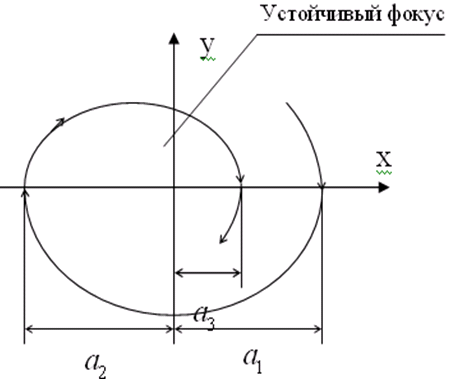
\includegraphics[width=0.4\linewidth]{30_coleb_zat.png}
\caption{Колебания с убывающей амплитудой}
\end{figure}


\item Расходящийся колебательный процесс.

\begin{equation}
x(t) = ae^{nt} \cos \omega t;
\end{equation}
\begin{equation}
y(t) = ae^{nt} \sqrt{\omega^2 + n^2} \sin[\omega t + \varphi(t) ].
\end{equation}

\begin{figure}[H]
\centering
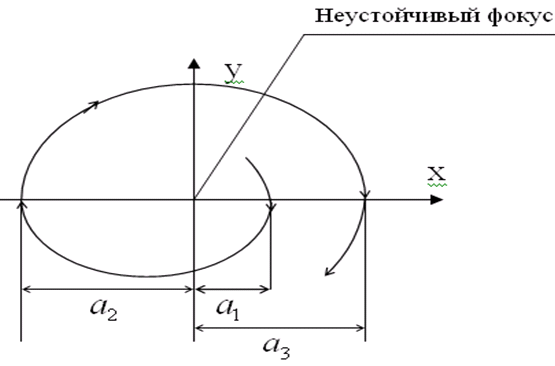
\includegraphics[width=0.4\linewidth]{30_coleb_rash.png}
\caption{Колебания с возрастающей амплитудой}
\end{figure}


\item Затухающие апериодические процессы.

\begin{figure}[H]
\centering
\includegraphics[width=0.8\linewidth]{30_aperiod_zat.png}
\caption{Переходный процесс и фазовая траектория затухающих апериодических процессов}
\end{figure}


\item Расходящиеся апериодические процессы.

\begin{figure}[H]
\centering
\includegraphics[width=0.8\linewidth]{30_aperiod_rash.png}
\caption{Переходный процесс и фазовая траектория расходящихся апериодических процессов}
\end{figure}

\end{enumerate}

% Вопрос 31 ---------------------------------------------------------------------------------------------------------------
\section{Показатели качества ЭС.}

Показатели качества продукции --- количественная характеристика определенного свойства продукции на определенном этапе жизненного цикла.

Показатели качества продукции делятся на следующие группы:
\begin{enumerate}
\item Назначения
\item Надежности
\item Технологичности
\item Эргономические
\item Эстетические
\item Стандартизация и унификация
\item Патентно-правовые
\item Экономические
\end{enumerate}

Единичный показатель качества --- показатель качества продукции, относящийся только к одному из её свойств. Комплексный показатель качества --- показатель качества продукции, относящийся к нескольким её свойствам.

% Вопрос 32 ---------------------------------------------------------------------------------------------------------------
\section{Управление качеством ЭС.}

Управление качеством продукции базируется на статических методах контроля, зародилось в 30-е годы в связи с переходом к массовому производству изделий. В связи с этим стали применять выборочный контроль продукции с оценкой его результатов статистическим методом.
Контроль качества базируется на статистических методах и развиваясь циклически проходит через определенные этапы (см. рис)
\begin{center} 
\includegraphics[width=0.6\textwidth]{32_Demming.png}\\
\end{center}

Управление качеством продукции базируется на статических методах контроля, зародилось в 30-е годы в связи с переходом к массовому производству изделий. В связи с этим стали применять выборочный контроль продукции с оценкой его результатов статистическим методом.

Контроль качества базируется на статистических методах и развиваясь циклически проходит через определенные этапы

Для эффективного обеспечения контроля качества необходимо участие всех, без исключения, работников предприятия. Такой контроль качества называется Тотальным(TQC). Был придуман и внедрен впервые в Японии 60х годах.

Среди статистических методов можно выделить 7 наиболее эффективных  и доступных:
\begin{enumerate}
\item	Расслоение графики (полигон, гистограмма, кумулятивная кривая)
\item	Расслоение общей изменчивости статистических данных с помощью дисперсионного анализа.
\item	Диаграмма Парето
\item	Причинно-следственная диаграмма
\item	Диаграмма разброса (поле корреляции)
\item	Контрольная карта
\item	Контрольный лист
\end{enumerate}


% Вопрос 33 ---------------------------------------------------------------------------------------------------------------
\section{Себестоимость и уровень качества ЭС.}

Зависимость себестоимости и уровня качества продукции можно в общем виде представить в виде следующего графика (рис.)

СП – затраты на материалы, комплектующие  изделия, оборудование, заработную плату, контроль и испытания и т.д. 
 \begin{figure}
 \centering 
 \includegraphics[width=0.7\textwidth]{33_Sebestoim.png}
 \caption{Слева -- зависимость себестоимости от уровня качества, справа --оптимальный уровень качества при затратах на изготовление и эксплуатацию.}
 \end{figure}
При повышении уровня качества от низкого до оптимального затраты растут медленно (х), поскольку производство легко справляется с заданными требованиями на уровень качества. По мере повышения УКП затраты (у) существенно возрастают. При дальнейшем повышении требований к УКП в конце концов достигается такой предел, когда ни оборудование, ни ТП, ни НТП и т.д. не в состоянии обеспечить требуемого (недостижимо высокого) качества. Затраты при этом устремляются в бесконечность.

Затраты на продукцию складываются из затрат на изготовление (проектирование и производство) и на эксплуатацию продукции (рис.).
Оптимальный уровень качества продукции - это такой уровень, выше или ниже которого производить продукцию экономически нецелесообразно.
При низком уровне качества продукции в сфере эксплуатации потребитель вынужден выделять дополнительные средства на ремонт, доработку и обслуживание продукции.
Высокий уровень качества продукции обуславливается ее высокой себестоимостью. 


\begin{enumerate}
\item Расслоение графики (полигон, гистограмма, кумулятивная кривая)
\item Расслоение общей изменчивости статистических данных с помощью дисперсионного анализа.
\item Диаграмма Парето
\item Причинно-следственная диаграмма
\item Диаграмма разброса (поле корреляции)
\item Контрольная карта
\item Контрольный лист
\end{enumerate}


% Вопрос 34 ---------------------------------------------------------------------------------------------------------------
\section{Корреляционная связь показателей ЭС.}

Диаграмма разброса применяется для исследования зависимости (корреляции) между двумя видами данных. Поэтому её часто называют полем корреляции.
С помощью диаграммы разброса удобно наблюдать процесс изменения параметра качества во времени при воздействии тех или иных факторов.

Совокупность точек на графике – диаграмма рассеяния.
С помощью диаграммы разброса можно определить имеется ли связь между параметрами и вид корреляции.(прямая корреляция, легкая прямая корреляция, обратная корреляция, легкая обратная корреляция, отсутствие корреляции, криволинейная корреляция.)

 \begin{figure}
 \centering 
 \includegraphics[width=0.8\textwidth]{34_Korelyacia2.JPG}
 \caption{Виды корреляции}
 \end{figure}
 
 Криволинейную корреляцию можно разделить на участки, имеющие прямолинейный характер, и исследовать каждый участок в отдельности.
 
 Степень связи может быть оценена: коэффициентом корреляции (прямолинейная), корреляционным отношением (криволинейная).
 
 Связь прямолинейную между Х и У можно найти:
 \begin{equation}
 Y-m_Y = r \cdot \frac{S_X}{S_Y} \cdot (X-m_Y),
 \end{equation}
 где r - коэффициент парной корреляции,
 \begin{equation}
 r = \frac{\sum_{i=1}^n (X_i - m_X)(Y_i-m_Y)}{(n-1) \cdot S_X \cdot S_Y},
 \end{equation} 
 \begin{equation}
 m_X = \dfrac{\sum_{i=1}^n X_i}{n}; S_X=\sqrt{\dfrac{\sum_{i=1}^n (X_i -m_X)^2}{n-1}},
 \end{equation}
 
  n - число пар наблюдений.
  
 $ -1 \leqslant r \leqslant 1$
 
 При |r|=1 – связь функциональная (зависимость между параметрами ввиде формул),
 
при |r|<1 – связь статическая. Каждому фиксированному значению Х соответствует ряд изменяющихся вместе с Х значений У и наоборот. Параметры Х и У считаются статистически зависимыми, если
\begin{center} 
  $\dfrac{\mid r \mid \cdot \sqrt{n-2}}{\sqrt{1-r^{2}}} \geqslant t_T = f(\alpha ; \nu = n-2)$\\
  \end{center}
  
Знак говорит о связи значений, если «-» то при уменьшении значения Х , У увеличивается и наоборот. Если «+» то при увеличении Х увеличивается и У.
  При r = 0 Х и У не связаны  между собой и не зависят друг от друга.

% Вопрос 35 ---------------------------------------------------------------------------------------------------------------
\section{Метод расслаивания <<4М>>.}

Простой и эффективный статистический метод, широко используемый в системе УК, - метод расслаивания

В основе метода – расслаивание статистических данных (т.е. группировка данных) в зависимости от условия их получения и обработка каждой группы в отдельности. Данные, разделённые на группы в соответствии с их особенностями, называют слоями (стратами), а сам процесс разделения на слои – расслаиванием (стратификацией). Существуют различные методы расслаивания, применение которых зависит от конечных задач. В производственных условиях обычно используется метод 4М, учитывающий факторы, зависящие от человека, машины, материала, метода. Расслаивание осуществляется:
\begin{enumerate}
\item по исполнителям – квалификации, полу, стажу работы и т.п.;
\item по оборудованию – году выпуска, марке, типу конструкции  и т.п.;
\item по материалу – месту производства, фирме-производителю и т.п.;
\item по способу производства 

\end{enumerate}

В результате расслаивания обязательно должны соблюдаться два условия:
\begin{itemize}
\item различия между значениями СВ внутри слоя должны быть как можно меньше по сравнению с различием её значений в не расслоенной исходной совокупности;
\item различие между слоями  должно быть как можно больше.
\end{itemize}	

При контроле качества изготовления изделий на практике возникает задача предполагаемого источника ухудшения качества продукции, когда разброс значений параметра качества около среднего значения возрастает. В случае нормального закона распределения контролируемого параметра качества такую информацию возможно получить путём расслаивания дисперсии с помощью дисперсионного анализа.

% Вопрос 36 ---------------------------------------------------------------------------------------------------------------
\section{Метод <<АВС-анализ>>.}

Метод служит для эффективности контроля качества изделия, для этого все изделия разбиваются по ценовым диапазонам (или иным критериям), составляется таблица,\\
\begin{center} 
  \includegraphics[width=0.7\textwidth]{36_Shapka.png}
  \end{center}
   и строится диаграмма Парето (по оси У откладывается относительная стоимость изделия в 
   \%
   , а по оси Х относительная частость изделий в
  \%). По результатам которой можно выделить три группы: группа А – наиболее дорогие изделия и её контроль должен быть наиболее строгим, группа С – наиболее дешевые изделия и её контроль упрощенный, все остальные изделия отнесутся к группе В и контроль качества должен быть средним.
  АВС-анализ широко применяется для контроля за производительностью труда, контроля денежных сумм, связанных со сбытом  и т.д.
  
\section{Виды статистического контроля ЭС.}
%Вопрос №37

Статистический контроль – это процесс установления соответствия между состоянием объекта и заданными на него нормами.\\
Контролем охватываются все этапы производства ЭС. В зависимости от стадии жизни изделия различают производственный и эксплуатационный контроль.

\underline{Производственный контроль} – (статический на стадии производства) охватывает все вспомогательные, подготовительные и технологические операции. В зависимости от места в цепи ТП произв контроль подразделяют на входной, операционный и приемочный.\\
\textit{Входной контроль} – контроль продукции поставщика. Материалы, комплектующие изделия подвергаются контролю на соответствие НТД.\\
\textit{Операционный контроль} – контроль продукции после завершения определенной операции.\\
\textit{Приемочный контроль} – контроль готовой продукции по окончании всех технологических операций.

\underline{Эксплуатационный контроль} – контроль, осуществляемый на стадии эксплуатации.\\
Часто статический контроль называют параметрическим контролем, потому что он базируется на контроле фактических значений параметров качества и сравнении их с запланированными значениями по НТД.

Перечисленные виды контроля могут быть как сплошными (100\%), так и выборочными.\\
Контроль по количественному признаку – регистрация точных числовых значений, измеряемых параметров качества.

Контроль по качественному признаку – выделяются категории к которым принадлежит контролируемое изделие. Частным случаем контроля по качественному признаку является контроль по альтернативному признаку – когда продукция разбивается на годную и не годную.
Летучий контроль – выборка из потока изделий в случайное время для контроля.

\section{Количественные показатели надежности ЭС.}
%Вопрос №38

Виды изделий:
	\begin{enumerate}
	\item По способу применения (изделия однократного и многократного действия);
\item	По способу обслуживания (восстанавливаемые и невосстанавливаемые изделия).
	\end{enumerate}
Восстанавливаемое ЭС -  изделие, изделия отказы которого устраняются путем ремонта (замены отказавшего элемента работоспособным). При этом само изделие состоит из невосстанавливаемых ЭРЭ (резисторов, конденсаторов, ИС) и узлов (собранных на гибридных и твердых схемах, микромодулях, микропроцессорах). Отказавшие ЭРЭ и узлы изымаются из изделия и заменяются на работоспособные.
Невосстанавливаемые являются изделия, не подлежащие ремонту в процессе эксплуатации.
\begin{itemize}
\item 	Показатели надежности  являются случайными величинами, т.к. все отказы случайные события
\item	Показатели надежности – функции времени.
	\end{itemize}
Показатели (их 5):
\begin{enumerate}


\item \underline{	Вероятность безотказной работы} p(t) – вероятность того что в заданном интервале времени (от 0 до t часов) в изделии не произойдет отказа.\\
p(t) = P(T>t), где Т – время безотказной работы, t – заданное время работы изделия.

Статистический расчет \\
\begin{equation}
p^{*}(t) = \frac{N(t)}{N_0} = \frac{N_0 - n(t)}{N_0} = 1- \frac{n(t)}{N_0}
\text{ где $N_0$ – общее число изделий, n(t) – число изделий отказавших за время t, N(t) – число изделий продолжающих работать после времени t.}\\
\end{equation}
$0 \leqslant p^{*}(t) \leqslant 1$.

Вероятность безотказной работы может быть и определена и для произвольного интервала времени (t1,t2). В этом случае говорят об условной вероятности безотказной работы
$P(t1,t2) = \frac{ P(t2)}{P(t1)}$
\item  \underline{	Вероятность отказа}q(t) - вероятность того что изделие откажет в течении заданного интервала времени (от 0 до t часов).
$q(t) = P(T \leqslant 1)$,
\begin{equation}
q(t) = 1-p(t),
\end{equation}
 вероятность отказа – противоположное событию безотказной работы.
 
Статистически значение находится по формуле\\
\begin{equation} q^{*}(t) = 1-p^{*}(t) = 1-1+\frac{n(t)}{N_0}=\frac{n(t)}{N_0},
\end{equation}
$0 \leqslant q^{*}(t)\leqslant 1$
\item	\underline{Частота отказов} f(t) – представляет безусловную плотность вероятности безотказной работы изделия. Она производная по времени от функции вероятности отказа\\
\begin{equation}f(t) = \frac{dq(t)}{dt} = -\frac{dp(t)}{dt} ,
\end{equation}
Частота отказа характеризует скорость изменения надежности (по вероятности безотказной работы) во времени, причем изменение происходит в сторону снижения надежности.

Статистически  она находится по формуле
\begin{equation}f^{*}(t) = \frac{n(t+\Delta t)-n(t)}{\Delta t \cdot N}= \frac{n(t)}{\Delta t \cdot N},
\end{equation} где $n(t+ \Delta t)$ – число отказавших изделий за время $ t+\Delta t$ \\
$f^{*}(t)$ – отношение числа отказавших изделий  в единицу времени t к общему числу изделий поставленных на испытания $N_0$.

\item \underline{Интенсивность отказов} $\lambda (t)$ – условная плотность вероятности безотказной работы.
\begin{equation} \lambda (t) = -  \frac{dp(t)}{dt} \cdot \frac{1}{p(t)} =  \frac{f(t)}{p(t)},
\end{equation}

Статистически интенсивность находят как\\
\begin{equation} \lambda^{*}(t)=\frac {f^{*}(t)}{p^{*}(t)}=\frac{n(\Delta t)}{\Delta t \cdot N(t)}
\end{equation}

Графическая зависимость интенсивности отказов от времени для большинства ЭС имеет вид\\
\begin{figure}[H]
\centering
\includegraphics[width=0.6\textwidth]{38_Zhizn2.png}
\caption{Зависимость интенсивности отказов ЭС от времени: I - 0-t1 период приработки изделия, II - t1-t2 период эксплуатации изделия, III - t2-$\infty$ период старения и износа изделия}
\label{fig:Zhizn}
\end{figure}
В 1 периоде отказы ЭРЭ, узлов  происходят из-за: некачественного монтажа, сборки, низкой надежности элементов, контактов , проводников.
Во 2 периоде число отказов стабилизируется , но оно не равно нулю.
В 3 периоде отказы изделия происходят из-за физического старения материалов и износа ЭРЭ, имеющие необратимый характер.
Для нахождения р(t) = F[$\lambda$(t)] проинтегрируем $\lambda(t)$,
\begin{equation}\int_0^t \lambda (t) =- \int_0^t \frac{dp(t)}{dt} \cdot \frac{1}{p(t)} ,
\end{equation}
\begin{equation} -\int_0^t \lambda (t)dt = \int_0^t \frac{dp(t)}{p(t)}, -\int_0^t \lambda (t)dt = \ln p(t) ,
\end{equation}
\begin{equation}
p(t) = e^{- \int_{0}^{t} \lambda(t)dt}
\end{equation}

Вероятность безотказной работы имеет экспоненциальный вид, аналогично может быть найдена условная вероятность безотказной работы за интервал времени (t1,t2)
\item \underline{	Средняя наработка до отказа}
Tcp(t) – время работы изделия до первого отказа.
\begin{equation}
T_{cp} (t)= \int_0^\infty p(t)dt,
\end{equation}
Статистически оно находится
\begin{equation}
T^{*}_{cp} (t) = \frac{1}{N_0} \sum_{i=1}^{N_0} t_i,
\end{equation}
где $t_i$ – время работы до отказа i-го однотипного изделия.
Рассмотрим расчет показателей надежности ЭС для 2 периода $ \lambda(t)=const = \lambda$
\begin{equation}
p(t)= e^{- \lambda t},
\end{equation}
\begin{equation}
T_{cp}(t) = \int_0^\infty p(t)dt= \int_0^\infty e^{- \lambda t}dt = \frac{1}{\lambda},
\end{equation}
Рассмотренные показатели надежности справедливы для невосстанавливаемых ЭС.
\end{enumerate}

\section{Последовательная модель надежности ЭС.}
%Вопрос №39

При последовательном соединении элементов расчет надежности производят по формуле %formula

 \begin{equation}
 P_A(t) = {\prod_{i=1}^{m}p_i(t) }
 \end{equation}
Для большего значения вероятности безотказной работы каждый элемент должен иметь значение вероятности безотказной работы близкой к единице.\\
$P_A(t)\leqslant1$,
 при увеличении количества компонентов в ЭС надежность его падает.(пример)
В тех случаях , когда нужна высокая надежность ЭС, а элементы имеют небольшое значения вероятности безотказной работы, применяют метод резервирования.

\section{Параллельная модель надежности ЭС.}
%Вопрос №40

При параллельном соединении элементов расчет надежности производят по формуле 
 \begin{equation}
 P_A(t) = {1- \prod_{i=1}^{m}[1-p_i(t)] }
 \end{equation}
% Вопрос 41 --------------------------------------------------------
\section{Основные этапы автоматизации:  их характеристики и особенности}

\underline{Этапы развития автоматизации}\\
\textit{Первый этап} - автоматизация цикла обработки с целью получения заданной формы, размеров и качества обрабатываемой поверхности, цикла сборки для фиксации сборочного соединения.

Средства автоматизации - ЧПУ обеспечивающие эффективное использование технологического оборудования только в крупносерийном и массовом производстве.

\textit{Второй этап} - наряду с автоматизацией цикла обработки (сборки) обеспечивается автоматизация загрузки и разгрузки основного технологического оборудования. Такое оборудование оснащено магазинами заготовок и готовых деталей в виде комплектов под сборку и загрузочными устройствами, приспособленными в обслуживанию определенной номенклатуре деталей, функции загрузки-разгрузки может выполнять ПР, установленный совместно с ЧПУ, который обеспечивает возможность использования оборудования в серийном производстве.

\textit{Третий этап} - предусматривает автоматизацию контроля за ходом выполнения техпроцесса и его оптимизацию. При этом выделяется 2 вида контроля:
\begin{itemize}
    \item проверки соответствия заготовок (комплектующих деталей при сборке), инструмента, состояния технологического оборудования установленным характеристикам с целью внесения коррекции настройкой оборудования или удаления из потока некондиционных деталей.
    \item проверка текущего состояния инструмента и оборудования путем измерения силовых, температурных деформаций и сравнения текущих параметров с эталонными.
\end{itemize}

Таким образом, учитывается влияние случайных и систематических факторов на характер тех. процесса.

\textit{Четвертый этап }- обеспечивается автоматизация переналадки оборудования на обработку (сборку) объектов производства другого назначения. Это возможно при использовании, к примеру, обрабатывающих и сборочных центров, оснащенными ПР с наборами сменных инструментов, захватных устройств, системы накопителей под номенклатуру обрабатываемых или собираемых узлов (деталей) и оснастки. В этом случае размер изготовляемой партии изделий не имеет значения, ограничивающего гибкость робототехнического производства, классификация (признаки классификации).

% Вопрос 42 --------------------------------------------------------
\section{Назначение, классификация и области применения роботов}

Можно разделить на 3 класса:
\begin{enumerate}
\item	манипуляционные или роботы манипуляторы;
\item	информационные;
\item шагающие
\begin{itemize}

\item  роботы-экзоскелеты (медицинские, роботы-усилители);
\item шагающие аппараты.
\end{itemize}
\end{enumerate}
Манипуляционные: 
\begin{enumerate}
\item	промышленные (универсальные, специальные, специализированные);
\item погрузочные манипуляторы;
\item	для экстремальных сред (космические, подводные, для радиоактивных сред, для токсичных сред, взрывобезопасные);
\item	медицинские;
\item	бытовые;
\end{enumerate}
Наиболее обширен класс роботов-манипуляторов.

Класс информационных роботов включает в себя аппараты для исследования космического пространства,подводного дна и т.п. Они предназначены для автоматического получения и передачи информации об исследуемых объектах.

Класс шагающих роботов включает в себя а), кто предназначены для восстановления двигательных функций человека или для технического усиления мощности двигательных конечностей здорового человека (б).

% Вопрос 43 --------------------------------------------------------
\section{Манипуляционные роботы: типы, характеристики, применение}

Они представляют собой техническую систему, заменяющую труд человека, в состав которого входят орган воздействия на окружающую среду, т.е манипуляционные устройства или манипулятор-это исполнит. Орган, имитирующий действие человеческой руки в достаточно широком диапазоне масштабов увеличения или уменьшения ее геометрических размеров и мощности.

Обобщенная функц. схема манипуляционного робота имеет следующий вид:
\begin{figure}[H]
\centering
\includegraphics[width=0.8\textwidth]{44_Manipul_robot.png}
\caption{Обобщенная функциональная схема манипуляционного робота}
\end{figure}

Различные группы манипуляц. роботов включают в себя ту или иную часть блоков и связей, составляющих обобщенную схему.

Манипуляц. робот м. иметь 1 или несколько манипуляторов. Движения манип-ров м. отличаться от движения руки ч/а. В суставах, звеньях манип-ров м. не только вращаться, но и перемещаться поступательно. М. изменяться длина некоторых звеньев. Кисть руки имитируется с пом. захвата (м.б. 2-хполый, 3-хпалый или более). На захвате м.б. установлены различные датчики.

Средства передвижения м.б. колесными, гусеничными, шагающими, плавающими и т.д.
Устанавливаемые датчики И. позволяют роботу ориентироваться во внешней среде.
По способу упр-я манипуляц. роботов разделяют на 3 группы: автоматич.,биотехнические, комбинированным управлением.

\textit{Автоматическими} манипуляц. роботами называют  устройства, ктр. действуют без непосредственного участия ч/а в упр-ии. Они прим-ся в тех случаях, когда манипуляц. устр-во удалено на значит. расст. от органов упр-я, либо когда очень высокий темп работ, опасны внешняя среда или объект действия, а ручное упр-е нецелесообразно.
Выделяют: I покол.(программн, интеллектуальные, адаптивные).

\textit{Биотехнич.} манипуляц. роботы – робот, в систему упр-я ктр-х включен человек-оператор. М.б.: командные – упр-ся оператором дистанционно с командного устр-ва с нажатием кнопок или с помощью упр-щей рукоятки.

\textit{Копирующие} манипуляц. роботы имеют задающий орган, геометрически подобный манипуляц-ому устр-ву. При этом способе упр-я привод каждого звена вместе с соответствующим датчиком образует дистанционно следящую систему. Если положения задающего органа и манипуляц. устр-ва совпадают, то последнее стремится к 0 ошибке по положению.

% Вопрос 44 --------------------------------------------------------
\section{Структура механизмов манипуляционных роботов и характеристики их геометрических свойств}

Механизмом называют механич. систему, предназначенную для получения требуемого движения 1-го или нескольких тел.

Основными элементами являются: звенья и кинематич. пары.

Звено-1 или неск жестко соединенных твердых тел, входящих в состав механизмов.
Звенья:
\begin{enumerate}
\item простые состоят из 1-го твердого тела;
\item составные – из нескольких твердых дел.
\end{enumerate}

Кинематич. пара – соединение двух смежных звеньев, допусккающие их относит. движение. Звенья м. соприкасаться пов-тями, линиями и точками.
Кинематич. пара м.б. плоской, если относит. движение сочлененных звеньев возможно лишь в параллельных плоскостях или в пространстве, если относительное движение сочлененных звеньев возможно в любом направлении.

С целью уменьшения потерь и увеличения износостойкости между звеньями вводят промежуточные элементы (ролики или шарикоподшипники). Такие совокупности образуют кинематич. соединение.

Кинематич. пары классифицируются по числу условий связи на относительное движение двух смежных тел или по числу степеней свободы. Каждое условие связи кинематич. пары не только устраняет относительную подвижность, но и позволяет передавать от звеньев к звеньям силовое воздействие.

Свободное тело в пространстве имеет 6 степеней своб:3 поступательные движения в направлении оси x,y,z, 3 вращательных движения относительно этих осей.

Если 1 звено превратить в стойку, то для 2-го звена в соответствии с конструкцией кинематич. пары: W=G-U, U-число связей, налагаемых кинематич. парой на относительно движения ее звеньев. При U=0 пара отсутствует, т.к. отсутствуют связи между звеньями. При U=6 относительного движения звеньев нет, т.к. они образуют 1 звено. Поэтому число условий связи кинематич. пар м. находиться в пределах от 1 до 5. Соответственно этому все кинематич. пары делят на 5 классов или на 5 родов по числу степеней свободы.

Кинематич. пары 1 и 2 классов в манипуляц-х роботах не применяются. Примеры кинематич. пар манипуляц. устр-в:
Класс 3, род 3 – 3 степени свободы, класс 4, род 2 – 2 степени свободы.

Кинематич. пара 3 класса 3 рода предст. собой шаровой шарнир , имеющий 3 степени свободы-вращение относительно каждой из осей.

 Кинем. пара 4 класса 2 рода м.б. реализована либо вращением одной из осей, указанных в системе коорд. и поступат. движ. Вдоль 1 оси, либо вращениие относит. двух взаимоперпендикулярных осей.

Кин. пара 5 класса 1 рода позволяет иметь лишь одно относит. движение-либо вращение, либо поступат. движение вдоль 1 оси.

Кинемат. цепью называют связанную систему звеньев, образующих кинематич. пару. Они бывают замкнутыми и открытыми. Замкнутая кинемат.цепь – такая цепь, в ктр.звенья входят не менее, чем в 2 кинемат. пары. Открытая кинем. цепь – цепь, в ктр. имеются отдельные звенья, входящие только в 1 кинем. пару.

Механизм манипуляц. робота представляет собой сложную открытую кинем. цепь, у ктр-х 1 звено обращено в стойку, а движение вых-х звеньев вполне опр-ся заданным движением входных звеньев.

Манипуляц. устр-ва предст. собой открытую кинематич. цепь, в ктр. число n подвижных звеньев всегда = числу кинематич. пар. Тогда число степеней свободы для механизма манипуляц-го устр-ва опр-ся как: \begin{equation}
W=3p3+2p4+p5
\end{equation}
\begin{equation}
n=p3+p4+p5
\end{equation}

Пространств. исполнит. механизмы м. иметь большое число степеней свободы во многих отношениях они аналогичны руке человека. Однако число звеньев чел. руки достаточно велико (n=19) и число степеней свободы W=27. В наст. время ни один механизм не обладает такими возм-тями . Однако при существующем уровне техники-это не так уже важно.

Характеристики геом-х св-в манип-х устр-в:
\begin{enumerate}
\item  \underline{Зона обслуживания}

У манипуляц-х устр-в выделяют базовую плоскость, плоскость ктр образована плечом и предплечием мнипулятора и в ктр м. располагаться одновременно оси всех его звеньев.

Зоной обслуживания манипуляц-го робота называют сов-ть точек базовой плоскости, ктр. м. достигать захват манипуляц-го устр-ва. Преимущественное распространение получили манипуляторы с упорядоч-м расположением звеньев кинематич-х пар , т.е. такие, когда имеется 1 пара смежных кинематически связанных звеньев, ктр обеспечивает перенос кисти в базовой плоскости в любую точку зоны обслуживания.

\item \underline{Рабочий объем} или рабочие зоны манипуляц-го устр-ва называют пространство , ограниченное поверхностью, огибающей все возможные положения захвата. Для обеспечения наиболее полного обслуживания любой точки необходим механизм манип-ра, исп-щий не менее 6 степеней свободы, из ктр-х 3-для перемещения кисти, 3-для ориентации захвата кисти. Тогда в зависимости от сочетания кинем. пар, обеспечивающих перемещения кисти различают 3 осн.формы рабочего объема:
\begin{itemize}
\item	прямоугольный, когда кисть пеермещается в пространстве с пом. Механизма с 3-мя поступат-ми кинем-ми парами 5 класса;
\item цилиндрич., когда исп-ся механизм с двумя поступательными и 1 вращательной кинем.парой;
\item сферический, когда исп-ся 2 вращат. и 1 поступат., либо 3 вращат. кинематич. пары.
\end{itemize}
\item  \underline{Движение манипуляц. робота} и его манипуляц-го устр-ва. Для манипуляц-х роботов вводят понятие глобальных, региональных и локальных движений.

К глобальным движениям робота относят его перемещ-я в пространстве с пом. средств передвижения.
Регион.движения робота-это движения по переносу кисти его манипуляц-го устр-ва в любую точку рабочего объема.

Локальные движения робота связаны с ориентацией кисти в пространстве и движение по захвату объектов действий, движение манипулятора в его рабочем объеме м. классифицировать:
\begin{itemize}
\item	Движение манипуляц-го устр-ва, несущего своб. объект и совершаемые в своб. объеме
\item	Целенаправленное движение манипуляц-го устр-ва по перемещению своб-го объекта, совершаемые в несвободном рабочем объеме
\item	Движение манипуляц-го устр-ва в своб. объеме, согласованные с движением объекта действия
\item	Движения манипуляц-х устр-в в несвоб.объеме, согласованные с перемещением объекта действий.
\end{itemize}
\item \underline{Маневренность}

Ключевой А и запястный кистевой механизм С имеют каждый 3 степени  свободы. Они позволяют ориентировать кисть 3 на нектр. Участки поверхности сферы с радиусом, равным пределе сумм длин плеча 1 и 2.
Кинематич.пара 5 класса в локтевом суставе В позволяет менять радиус сферы и доставлять захват в любую точку сферического рабочего объема.
Если зафиксировать захват 4 неподвижные точки. Манип. устр-во будет иметь возможность совершать круговое движение плечами 1 и 2. Т.о. св-ва манип-го устр-ва м. иметь подвижность при фиксированном захвате называется маневренностью. В рассм-вом случае механизм сохраняет 1 степень свободы, что оперделяет степень маневренности манип. устр-ва.

Повышение числа степеней маневренности позволяет выполнять движения более сложных классов, сужает мертвые зоны манип-го устр-ва и увеличивает свободу действий оператора.

Перестановка кинем. пар в данном устр-ве, н-р, А вместо В не меняет число степеней свободы, но при фиксированном захвате превращение манипуляц. устр-во в ферму и механиизм теряет свою маневренность.
\end{enumerate}

% Вопрос 45 --------------------------------------------------------
\section{Приводы манипуляторов и роботов: классификация, особенности применения}

В зависимости от используемого вида энергии приводы подразделяют на гидравлические, пневматические, электрические и комбинированные (например, электрогидравлические, гидропневматические и др.) Часто их применяют в комбинации, например, в звеньях манипулятора большой грузоподъемности используют гидравлический привод, а в его захватном устройстве — более простой и маломощный пневматический.

\underline{Пневматические} приводы применяются в 20…30\% (по другим оценкам в 40-50\%) серийно выпускаемых ПР. Их используют  для легких и средних (по грузоподъемности до 20 кг) ПР при числе степеней подвижности 2…3. Погрешность позиционирования в этих приводах не превышает ± 0,1 мм. Скорость ведомого звена привода при линейном перемещении составляет до 1000 мм/с, при угловом – до 60 об/мин. Они имеют простую конструкцию, низкую стоимость и достаточно надежны в работе.

Вследствие низкой регулировочной способности их мало используют в позиционных и контурных режимах работы, и они имеют цикловое управление, как простейший вариант позиционного (задается две точки – начало и конец перемещения).

\underline{Гидравлические} приводы применяются в 30\% серийно выпускаемых средних и тяжелых ПР при числе степеней подвижности 3…4. Погрешность позиционирования в этих приводах не превышает ± 0,5 мм при скорости линейного перемещения до 0,8…1200 мм/с. Эти приводы имеют сложную конструкцию, высокую стоимость изготовления и эксплуатации. Гидравлический привод имеет хорошую регулировочную способность, и его используют в ПР с позиционным и контурным режимом работы.

\underline{Электрические} приводы используются в 40…50\% серийно выпускаемых ПР со средней грузоподъемностью и числом степеней подвижности 3…6. Точность позиционирования электрического привода достигает значений до ± 0,05 мм. Их применяют как в позиционном, так и в контурном режимах работы. 

Преимуществами электроприводов являются более высокая экономичность, КПД, удобство сборки и хорошие регулировочные свойства. 

Как правило, в электроприводах используют синхронные, шаговые и двигатели постоянного тока. Асинхронные двигатели применяются реже, что связано с трудоемкостью управления частотой вращения.

\underline{Комбинированные} приводы позволяют максимально использовать достоинства отдельных типов приводов. Чаще всего в промышленных роботах применяют комбинацию пневматического и гидравлического приводов (пневмогидравлические и гидропневматические), а также электрического и гидравлического (электрогидравлические). В конструкциях ПР пневмогидравлические приводы имеют ограниченное применение. В них в качестве исполнительного органа используется пневмоцилиндр, а стабилизация его скорости и гидравлическая фиксация осуществляется гидросистемой.

В гидропневматическом приводе в качестве исполнительных двигателей применяют гидродвигатели, а пневмосистема применяется для создания необходимого давления в гидросистеме, что позволяет отказаться от гидронасосных станций.

% Вопрос 46 --------------------------------------------------------
\section{Конструкции схватов промышленных роботов, особенности применения}

Промышленный робот (ПР) – это универсальное, автономное и автоматическое устройство с памятью и программным управлением, предназначенное для воспроизведения двигательных и некоторых умственных функций человека при выполнении основных и вспомогательных производственных операциях.
Основной частью ПР являются манипуляторы.

Под конструкцией роботов понимается конструктивное исполнение их механической системы.
В общем виде их механическая система состоит из следующих элементов:
\begin{itemize}
\item опоры, в виде основания или передвижных тележек напольного или подвесного типа;
\item корпуса робота различной формы с вмонтированными в него механизмами подъема и поворота руки и перемещения робота;
\item корпус руки робота с вмонтированными в него механизмами перемещения руки, звена, а в некоторых случаях, и захвата руки;
\item руки робота с одним или несколькими звеньями;
\item захватного устройства.
\end{itemize}

Захватные устройства служат для захватывания, базирования и удержания объекта в определенном положении. Эти объекты могут иметь различные материалы, форму, объем, массу. Обычно, в зависимости от этих показателей робот в пределах своей области применения имеет определенный набор ЗУ.
При необходимости робот оснащают специальными ЗУ в виде присосок, губок и другие для захвата специальных объектов. При этом, для надежности захвата применяют такое усилие, которое необходимо для удержания объекта, но не оставляло бы следов губок на его поверхности и не изменяла бы форму объекта.

Классификация ЗУ:
\begin{enumerate}
\item	По способу удержания объекта:
\begin{itemize}
\item	схватывающие
\item	поддерживающие
\item	удерживающие
\end{itemize}
\item	По принципу действия:
\begin{itemize}
\item 	механические
\item	с эластичными губками или камерами
\item	вакуумные
\item	магнитные
\end{itemize}
\item	По характеру базирования объекта:
\begin{itemize}
\item	центрирующее
\item	базирующее
\item	фиксирующее
\item	способное к перебазированию
\end{itemize}
\item	По степени специализации ЗУ:
\begin{itemize}
\item	универсальные (с широким диапазоном захвата)
\item	многоцелевые ( приспособленные для захвата по определенной номенклатуре поверхностей)
\item	целевые (предназначены для захвата только определенной группы деталей)
\item	специальные ( для определенного объекта)
\end{itemize}
\item	По рабочему диапазону:
\begin{itemize}
\item	широкодиапазонные для захвата различных поверхностей
\item	узкодиапазонные
\end{itemize}
\item	По наличию дополнительных устройств и механизмов:
\begin{itemize}
\item	без устройств
\item	с устройствами для ориетационных перемещений
\item	с приспособлением для выполнения технологических операций
\end{itemize}
\item	По числу рабочих позиций:
\begin{itemize}
\item	однопозиционный
\item	многопозиционный
\end{itemize}
\item	По характеру работ ЗУ:
\begin{itemize}
\item	последовательно
\item	параллельно
\item	комбинированный
\end{itemize}
\item	По виду управления ЗУ:
\begin{itemize}
\item	неуправляемый
\item	командный
\item	адаптивный
\item	жесткопрограммный
\end{itemize}
\item	По характеру крепления руки робота:
\begin{itemize}
\item	не сменяемые
\item	сменные
\item	быстросменные
\item	пригодные для автоматической смены.
\end{itemize}
\end{enumerate}

К ЗУ предъявляются требования общего характера и специальные, связанные с конкретными условиями эксплуатации.

К числу обязательных:
\begin{itemize}
\item	надежность захватывания и удержания объекта;
\item	стабильность базирования;
\item	недопустимость разрешения объекта.
\end{itemize}

Прочность ЗУ должна быть высокой при малых габаритных размерах. Особое внимание должно быть обращено на надежность крепления ЗУ к руке ПР.

К ЗУ работающих в условиях серийного производства существуют дополнительные требования:
\begin{itemize}
\item	возможность захватывания и базирования деталей в широком диапазоне массы, размеров и формы;
\item	обеспечение захватывания близко расположенных деталей;
\item	легкость и быстрота замены ЗУ.
\end{itemize}

В ряде случаев необходимо автоматическое изменение усилия удержания деталей.
ЗУ является основным рабочим органом робота, имеет очень разнообразные схваты, поэтому разработана стандартная таблица основных типов объектов, т.е. деталей:
\begin{enumerate}
\item Для деталей типа тел вращения:
\begin{itemize}
\item центрирующие
\item	базирующие
\item	с эластичным покрытием
\item	вакуумные.
\end{itemize}

Причем, здесь различаются ЗУ двух типов: для деталей типа втулок и типа валов, причем в последнем случае применяются только центрирующие ЗУ или захватные по наружному зазору.
\item Для плоских деталей, применяются, в основном, базирующие.
\item Для деталей коробчатой формы, те же, что и в первом случае (того же типа), кроме центрирующих.
\item Для нессиметричных деталей, те же, кроме центрирующих и эластичных, В основном, эти детали обрабатываются со спутниками и в зависимости от формы спутника.
\end{enumerate}

% Вопрос 47 --------------------------------------------------------
\section{Проектирование  архитектуры интегрированной компьютерной системы управления }

Целью ИКСУ является обеспечение условий для взаимосвязанного согласованного управления конструкторско-технологической подготовки произ-ва и упр-я производственными и технол-ми процессами. Методология проектирования таких систем –разделение объекта автоматизации на части, позволяющей осущ-ть эффективную автоматизацию ккаждой из них.


Применительно к иерархически организованных СУ различают горизонт. и вертик. интеграцию. В общем случае, горизонт. интеграция предполагает объединение АС 1-го уровня.Н-р, АС проектных работ производственного процесса.

Вертикальное-объединение разных уровней, в частности, вертик. Интеграция предполагает объединение САПР, автоматизации тех. процесса, а также корпоративных систем(экон-х, финансовых упр-ий персоналом) в единую интегрированную инф. Сеть, что обеспечивает обмен данными между всеми подразделениями упр-ческого уровня.

В наст. время вертик. интеграция формируется путем организации потоков И. от нижнего уровня (датчики, контроллеры АСУТП), от КД САПР во внутр. выч. сети участков и цехов(MES) и далее выч.сети предпр. в целом(ERP).

Сущность технологии открытых систем состоит в формировании среды, вкл-щей ПО, аппар.ср-ва, службы связи интерфейса, форматы данных и протоколы, обеспечивающие переносимость, масштабируемость и взаимосвязь приложений и данных. Сов-ть этих качеств достигается исп-ем общепризнанных стандартов на ИТ. Основным приемом построения служит национ.стандартизация или построение профиля.

Профиль-согласов. набор базовых стандартов, предназначенные для решения какой-либо задачи или класса задач.

В основе современных архитектур лежат 2 группы моделей: 
\begin{enumerate}
\item модель объектов данных с описанием И.,циркулирующей в ИКСУ;

\item операц.модели, опр-щие процессы преобраз.И.
\end{enumerate}
Для любых из таких моделей выделяют 4 общие группы стандартов:
\begin{enumerate}
\item стандарт на уровни;
\item стандарт на инф.потоки;
\item стандарт на интерфейсы; 
\item стандарт на операции и функции
\end{enumerate}

\textit{S-88, MES, S-95, OPC,ODBC, SQL, CALS, PLM}.

S-88 этот стандарт направлен на увелич.гибкости и прозрачности оборудования  и ПО. Он обслуживает batch-процессы и устанавливает рекомендации по реш.задач, связанных с упр-ем обор-я, безоп-тью, произв.рисками  и контролем производственных операций. Batch-процесс опр-ся как процесс выпуска конечного кол-ва продукции на основе обработки конечного кол-ва входных материалов в соответствии с указанной рецептурой на одной или более единицах оборудования, т.е. в отличие от непрерывного производства эти процессы основаны на использовании ограниченного кол-ва материала. Такие процессы характерны для гибких производственных систем.

В соответствии с требов-ми стандарта ISA S88.01-1995 при проектировании ИКСУ д.б. разработана модель состояний гибкой произв. системы и ТП в целом. Поведение оборудования планируется в виде диагарммы состояний. Т.о., в любой момент времени оборудование м. находиться в 1-м из предполагаемых состояний-остановка, сброс, пуск, работа, подготовка, авария и др.При исп-ии рекомендации данного стандарта контроллер будет исп-ть виртуальную машину состояний для опр-я состояния оборудования в любой момент времени.

ISA S-95 отвечает за решение задач операц-го менеджмента ср-вами инф-х систем. Он опр-ет интерфейсы между бизнес-функциями и произв-ми операциями и служит для интеграции соврем-х систем упр-я. Стандарт описывает модель производственных операций, получившую развитие в системах для исполнения произв. деятельности и содержит примеры док-та отчетности аналитических зависимостей, исп-мых для оценки эфф-ти произ-ва.
%Вставить картинку про 4 уровня.
\begin{figure}[H]
\centering
\includegraphics[width=0.8\textwidth]{47_Urovni.jpg}
\caption{Иерархическая модель упр-я согласно ISA-95}
\end{figure}

В 1 части ISA95.00.01 рассм-ся многоуровневая модель обмена И. и связи между ур.4 и 3 (производств.подразделения). 2 часть станд.определяет форматы обмена данными через эти связи в соответствии со схемой взаимодействия . Здесь определены форматы документов для обмена И.по оборудованиям, материалам, персоналам, технологии изготовления, эффективности ТП. 3 часть стандарта ISA95 описывает модели и действия, хар-ные для упр-я произв-вом(ур.3), ктр. обычно поддерживаются след-щими системами: исполнение произв. деят-ти (MES). контроля качества (LIMS) и автоматизированного упр-я активами предприятия (EAM).

Модель произв-ва приводится в действие плановым производством , по ктр-м составл-ся детальные графики, содержащие рабочие задания, действия и события.

Модели деят-ти при упр-ии произ-ми процессами рассмотрены в 4 части стандарта. 5 раздел стандарта посвящен обмену между бизнес-приложениями и производством. В упр-ии произв-ми процессами входят функции упр-я персоналом, обор-ем и материалами. Имеются функции для упр-я рецептурой и технологией произв-ва.

MES-исполнит.система произв-ва.Эти системы решают задачи синхронизации, координируют, анализируют и оптимизируют выпуск продукции.

OPC-стандарт подключаемости компонентов в компь.СУ. Они разработаны с целью сокращения затрат на создание и сопровождение приложений промышленной автоматизации. Их применение решает вопрос обмена данными с устр-вами разных производителей ИМС разными протоколами обмена данными. OPC-это программная технология на базе W-s технологии, представляющей единый интерфейс для упр-я объектами автоматизации. OPC DA описывает набор функций обмена данными в реальном времени с прогр.логическими контроллерами, ЧПУ и др. OPC AE- функции уведомления по требованию о различных событиях(ававрийные ситуации).

Применение OPC предоставляет разработчикам универс.фиксированный интерфейс обмена данными с любыми устр-вами. Разработчики устр-в ввода-вывода дополняют их спец.программой, реализующей интрефейс.

\textit{Достоинства OPC}:

Если заменяется какой-л компонент СУ, то нет нужды корректировать др.ПО, т.к.при замене драйвера поверх нее б.функционировать инсталлирование OPC. При включении нового компонента необходимо правильно сконфигурировать его на программном уровне. Если в систему добавить новую программу, необходима только конфигурация OPC-клиента.

CALS-архит.поддержка сбора данных в течении жизненного цикла продукции. Она обеспечивает единообразные способы упр-я процессами и взаимодействия всех участников этого цикла:заказчиков продукции, поставщиков и производителей экспл-ции и ремонтного персонала.

На предприятии с CAL-технологией реализуется в соответствии с требованиями системы международного стандарта, регламентирующих правила указанного вз-я преимущественно посредством электронного обмена данными.

Применение CALS-технологии позволяет существенно сократить объем проектных работ, т.к. описание составных частей оборудования, машин и систем, проектировавшихся ранее хранится в унифицированных форматах данных, доступных любому пользователю технологии CALS. Главная задачарешения-обеспечения единообразного описания и интерации результатов независимо от места и времени их получения в общей системе. При этом структура проектной технологич. и экспл. док-ции, языки ее представления д.б.стандартизованы, тогда становится реализумой успешная работа над общим проектов разных коллективов, разделенных во времени и в пространстве и использующих разные системы. 1 и та же КД м.б.использована в разных продуктах, а технологическая документация адаптирована к разным производственным условиям.

Для обеспечения инф.интеграции в качестве форматов данных используют стандарты ГОСТ ИСО 10303. В CALS входят также стандарты электронного обмена данными, электронные ТД и руководства для совершенствования процесса.

ODBC-это программный интерфейс доступа к БД, он позволяет единообразно оперировать с разными источниками данных, не учитывая особенности взаимодействия в каждом конкретном случае.Это достигается благодаря тому, что поставщики различных БД создают драйверы, реализующие конкретные дополнения функций ODBC с учетом особенностей их продукта.

SQL-язык структурированных запросов, универс.компь.язык для создания, модификации и упр-я данными в реляционных БД.Это язык манипулиров-я данными , ктр. позволяет описывать условия поиска И., не задавая для этого последовательность действий.

PROFINET предназначендля коммуникационной части систем промышленной автоматизации.Он обеспечивает доступ к устр-вам полевого уровня (датчики) со всех уровней упр-я предприятием. Стандарт позволяет выполнять широкий обмен данными и использует стандарты вплоть до полевого уровня: практически все стандарты Ethernet, промышленный протокол CAL.Все они м.б. интегрированы в профильную единую сеть без модификации установленной аппаратуры.

PROFINET использует стандарт TCP/IP для выполнения операций настройки параметров, конфигурирования и диагностики.Обмен данными в реальном масштабе времени выполняется через стандартные каналы связи Ethernet параллельно со стандартными вариантами обмена данными

% Вопрос 48 --------------------------------------------------------
\section{Описание технологического процесса как объекта автоматизированного управления }

Любое производство состоит из множества технологических операций, каждая из ктр-х служит для решения общей задачи выпуска продукции. Даже если большинство технологических операций упр-ся АС(РТК,АСУТП), то это оказывается недостаточной для решения задач упр-я производством, т.к. эти автоматизированные участки обладают собственной логикой работы и оперируют собственным набором данных.

\begin{figure}[H]
\centering
\includegraphics[width=0.6\textwidth]{48.jpg}
\caption{Технологический процесс}
\end{figure}

На рис. показаны типовые каналы упр-я и наблюдения за ТП. Фактически каналы упр-я и наблюдения в реальных технологических модулях, представляющих собой их различную комбинацию.

По функциональному назначению в СУ м. выделить 5 каналов упр-я,ктр. осуществляют разные по характеру воздействия на технологическую систему. 
Канал С1 связан с осуществлением разнообразных дискретных операций (вкл.,выкл. приводов). Число подобных операций м. достигать нескольких сотен и упр-я осущ-ся от спец-го машинного контроллера.

Канал С2 осущ-ет упр-е движ-ми рабочих органов. В зависимости от геометрии изделия на этом уровне м. осущ-ся линейные и круговые перемещения рабочих органов.
С3 отвечает за авоматич. коррекцию формообразующих движений. На этом уровне по результатам измерения обработанных деталей вводятся дополнит. корректирующие возд-вия с целью обеспечения заданной точности.

Каналы С4 и С5 применяются с целью обеспеч-я качества обработки.

Канал С4 связан с активным контролем деталей в процессе обработки, по результатам измерения, отклонений размеров деталей в следствии износа инструментов или деформации осущ-ся под наладкой.

Канал С5 соответствует уровню адаптирования упр-я, осущ-го по результатам измерения силы моментов, деформации с целью изменения параметров процесса обработки.
Для формирования упр-я м. использоваться спец.каналы наблюдения. Различают след.уровни наблюдения:

01 соответствует обнаружению событий об исполнении той или иной команды (осведомит.сигналы, поступающие в систему упр-я для выполнения след.команды).

02-уровень измерения линейных и круговых перемещений. Измерение перемещения и их производных осуществляется измерительными преобразователями различной физической природы.

03-диагностика состояния оборудования, т.е. формирование упр-щих возд-вий м.участвовать и дополнит.измерит.И.,н-р, о параметрах деталей до и после обработки, от состоянии самого технологического модуля, его узлов и т.д.

04-06 контролирование состояний материального потока на входе ТП,н-р,геом. параметры заготовки и инструменты.
Ур.07 и 08 контролируют состояние энергетического процесса. Число уравнений наблюдения м.б.значительно больше уравнения упр-я. Чем более ответственный и качественный ТП, тем больше уровней наблюдения требуется для упр-я технологическим процессом.

% Вопрос 49 --------------------------------------------------------
\section{Описание производственного процесса как объекта автоматизированного управления: реализация АРМ различных уровней}

Описание ПП в целом м.б.представлено в виде карты основных бизне-процессов, на каждый из ктр-х составляется спецификация. Функциональная модель бизнес-процессов представляет собой многоуровневую систему взаимосвязанных диаграмм, содержащую полное описание процессов жизненного цикла произв-ва продукции.

При этом вход I представляет собой то, что перерабатывается процессом, выход О-результат переработки, упр-е С-И., необходимая для выполнения процессов и механизм М –обеспечение выполнения процессов с использованием его оборудования(построение функциональных моделей регламентируется Р50.1.028-01).Стандартами MES и S95 установлены 8 базовых бизне-процессов

\begin{figure}[H]
\centering
\includegraphics[width=0.6\textwidth]{49_proizv_proces.jpg}
\caption{Производственный процесс}
\end{figure}

Из перечня задач, котор.д.решаться в рамках выполнения этих базовых бизнес-процессов м.б.выделены те, кoтoр.д.б.решены системой интегрированного компь-го упр-я с использованием АРМ различного назначения.

АРМ SCADA-мастера в общем случае д.решать следующие задачи:
\begin{enumerate}
\item диагностирование состояний технологического оборудования;
\item упр-е оборудованием посредством экранных форм (в режимах пуска, останова работы и т.п.);
\item подключение и визуализация заявок на производство продукции;
\item контроль над процессом автоматического изготовления;
\item архивирование технологических и расчетных параметров;
\item представление оперативной И.о выполнении сменных заданий;
\item подготовка отчетов о фактическом использовании оборудования.
\end{enumerate}
АРМ SCADA в диспетчеризации производства:
\begin{enumerate}
\item	отслеживание выполнения операции технол. требований;
\item	отслеживание выполнения заказов, объема и партий;
\item	контроль в реальном времени выполнения работ в соответствии с планом;
\item	анализ производительности;
\item	формирование отчетной документации;
\item	контроль состояния и распределения ресурсов;
\item	отслеживание занятости оборудования.
\end{enumerate}
АРМ SCADA технолога д.вып-ть след.функции:
\begin{enumerate}
\item управление качеством продукции:представление данных измерений о качестве продукции, собранных с технологических линий;
\item мониторинг И.о ходе ТП;
\item отслеживание предупредительной и аварийной сигнализации;
\item оповещение оператора об аварийных и внештатных событиях;
\item представление действий об исправлении ситуаций на основе зависимости и статистических данных;
\item контроль состояния и распределения ресурсов:отслеживание занятости оборудования и коррекция настроечных параметров и задач, сбор и хранение данных, отслеживание историй продукта (где и в каком порядке велась работа с данной продукцией)
\end{enumerate}
АРМ диспетчера по обслуживанию оборудования:
\begin{enumerate}
\item	отображение состояния технологического оборудования и всего комплекса аппаратных средств;
\item	отображение графика ремонтов, формирование заданий и контроль выполнения ремонтных работ;
\item	отслеживание аварийной ситуации в ТП;
\item	отслеживание наработки оборудования.
\end{enumerate}
АРМ менеджера или руководителя:
\begin{enumerate}
\item отслеживание графика изготовления продукции по каждому контракту;
\item	контроль номенклатуры и объемов полуфабрикатной продукции в незавершенном производстве;
\item	контроль планирования и отслеживания выполнения планов по производству
\item	отслеживание решений оперативного планирования.
\end{enumerate}


% Вопрос 50 --------------------------------------------------------
\section{Выбор датчиков технологического процесса: типы измерительных устройств,  подключение.}

При их выборе в ПЗ необходимо провести следующие расчеты исследования:
\begin{enumerate}
\item тип датчика,
\item точность или погрешность измерения,
\item диапазон измерения,
\item единицы измерений,
\item диапазон выходного сигнала датчика,
\item условие эксплуатации(защищенность ВГП,различные требов.к источникам питания, помехозащищенность и т.д.), 
\item интерфейсы связи с компь.средой,
\item стоимость(в т.ч.затраты на экспл-цию).
\end{enumerate}
Интерфейсы выходных сигналов измерительных приборов:
\begin{enumerate}
 \item по типу вых.сигнала:
 \begin{itemize}
 \item аналоговые(электросигнал,емкость,частота,ток: 0-20мА, 4-20мА, 0-5мА; напряжение, сопротивление),
 \item цифровые(двоично-десятичный код, RS232,RS485,HART-протокол,промышленные сети);
 \end{itemize}
\item вторичные измерительные преобразователи(измерит.мосты, самописцы, программируемые логич.контроллеры и др.)
\end{enumerate}
Первичный измерит.преобразователь (ПИП) с токовым аналоговым выходом имеет встроенный источник тока с некоторым внутренним сопротивлением.Источник тока упр-ся функцией f(x) измерения параметров ч:

Ток поступает в линию связи и на входном нагрузочном резисторе ВИП создает соот ветствующее падение напряжения,ктр.далее преобразуется в цифровое значение измеряемого параметра ч. ИП данного вида имеют унифицированные вых.сигналы постоянного тока в различных диапазонах (0-20мА,4-20мА,0-5мА). При этом минимальному значению тока соответствует миним.значение измеряемого параметра. Чаще всего при токовом сигнале 4-20мА применяют двухпроводную схему подключения. При сигнале 0-20мА-4-хпроводные.

Применение унифицированных сигналов регламентировано ГОСТ 26.011-80. ПИП с цифровым вых.сигналом имеет, как правило, гальванически развязанный выход с открытым коллектором транзистора или параллельным «сухим» контактом, питание ктр-го производится со стороны источника тока, встроенного в ИП. При этом, в зависимости от того,закрыт или открыт выход ПИП величина тока в линии связи имеет либо мах, либо миним.значение тока. Последовательность «замыканий/размыканий» вых.цепи ПИП порождает последовательность токовых двоичных импульсов определенной частоты и длительности, ктр.исп-ся либо для цифрового представления измеряемого параметра, либо для дискретного (вкл/выкл)

Цифровой ИП м.иметь след.вых.сигналы:
\begin{enumerate}
\item выход с токовой петлей (соединение),
\item выход по интерфейсу RS232 и подключение по RS485,
\item ПИП с HART-выходом,
\item ИП с полевой шиной.
\end{enumerate}

% Вопрос 51 --------------------------------------------------------
\section{Теорема Котельникова (теорема отсчетов). Квазидетерминированные сигналы.}

В теории и технике сигналов широко используется теорема Котельникова (теорема отсчетов): если наивысшая частота в спектре функции $s(t)$ меньше чем $f_m$ , то функция $s(t)$ полностью определяется последовательностью значений в моменты, отстоящие друг от друга не более чем на $1/2 f_m$ секунд.

В соответствии с этой теоремой сигнал s(t), ограниченный по спектру наивысшей частотой $\omega_m = 2\pi f_m$, можно представить рядом:
\begin{displaymath}
S(t) = \sum_{i=1}^{n}S(kt) \cdot \frac{\sin \omega (t-\frac{n}{2 f_{max}}) }{\omega (t-\frac{n}{2 f_{max}})}
\end{displaymath}
 
где $1/2f_m=\Delta t$ — обозначает интервал между двумя отсчетными точками на оси времени;

а $s(n/2f_m)=s(n\Delta t)$ — выборки функции $s(t)$ в момент времени $t=n\Delta t$.

В реальных условиях $f_\text{дискр} = 2f_{max} \cdot k \cdot n \cdot m$

Где $k$ – коэффициент запаса (1...6);

$n$ – количество разрядов;

$m$ – количество каналов.\\

\underline{Квазидетерминированные сигналы.}

Квазидетерминированные модели – модели, в которых значение одного или нескольких параметров априорно неизвестно.

При описании квазидетерминированных сигналов широко используют понятие элементарного сигнала. 
К элементарным относятся: постоянный сигнал, единичный импульс и синусоидальный сигнал.
\begin{enumerate}
\item Постоянный сигнал представляется соотношением $x = A$, где $A = const$. Единственным параметром постоянного сигнала является значение $A$.
\item Единичный импульс описывается математической моделью вида $x=d(t-t_u)$,
где $d(t-t_u)$ - дельта-функция, принимающая значение 0 при $t \neq t_\text{и}$ и бесконечность при $t=t_\text{и}$.
\item Гармонический сигнал описывается моделью вида: 
\begin{displaymath}
x(t)= A\cos (\omega t+\varphi)=A\cos (\frac{2\pi}{T} t+\varphi)
\end{displaymath}

и имеет три параметра: амплитуду $A$, частоту $\omega$ (или период $T$) и начальную фазу $\varphi$.

Периодические сигналы могут быть представлены путём разложения их в ряд Фурье:
\begin{displaymath}
x(t)= \frac{A_0}{2} \sum_{k=1}^{\infty} A_k\cos (k \frac{2\pi}{T} t-\varphi_k)
\end{displaymath}

т.е. ряд представлен элементарными гармоническими сигналами.
\item Последовательность прямоугольных импульсов. Для периодических импульсных сигналов определяют производный параметр - скважность импульсов: $q=T/t_\text{и}$.
\end{enumerate}

% Вопрос 52 --------------------------------------------------------
\section{Преобразование измерительных сигналов. Виды модуляций.}

Передача информации с помощью тех или иных физических процессов осуществляется путем определенного изменения значений их параметров. Подобные операции называются модуляцией. При модуляции мгновенное значение первичного измерительного сигнала управляет одним или несколькими (сложная модуляция) параметрами вспомогательного сигнала, называемого несущим. В качестве несущего сигнала в измерительной технике используют:
\begin{enumerate}
\item постоянный сигнал $z(t) = x_m$ ,
\item гармонический сигнал $z(t) = x_m \cos (\omega t + \varphi)$,
\item периодическую последовательность импульсов.
\end{enumerate}

В соответствии с выбором носителя и информативного параметра различают следующие виды модуляции:
\begin{itemize}
\item ПМ — прямая модуляция, обеспечиваемая изменением значения постоянного сигнала; 
\item AM — амплитудная - $a(t)=A(t)\cos(\omega_0t+\varphi_0)$;
\item ЧМ — частотная - $a(t)=A\cos(\omega(t)t+\varphi_0)$;  
\item ФМ - фазовая - $a(t)=A\cos(\omega_0t+\varphi(t))$ модуляции, обеспечиваемые воздействием на соответствующий параметр гармонического несущего сигнала; 
\item АИМ — амплитудно-импульсная;
\item ЧИМ — частотно-импульсная;
\item ВИМ — время-импульсная;
\item ШИМ - широтно-импульсная;
\item ФИМ - фазоимпульсная;
\item СИМ — счетно-импульсная;
\item КИМ — кодоимпульсная модуляции, обеспечиваемые воздействием на соответствующий параметр периодической последовательности импульсных сигналов, используемых в качестве несущих.
\end{itemize}

Модулированное колебание имеет спектр, структура которого зависит как от спектра передаваемого сообщения, так и от вида модуляции. Основным параметром амплитудно-модулированного колебания является глубина модуляции. Отношение $M=\Delta A_m/A_0$ называется коэффициентом модуляции.

При изменении частоты всегда изменяется фаза колебаний, а при изменении фазы меняется частота, поэтому ЧМ и ФМ имеют общий характер, иногда их объединяют под общим названием угловой модуляции.

\begin{figure}[H]
\centering
\includegraphics[width=0.7\textwidth]{52.jpg}
\caption{Виды модуляции}
\end{figure}

% Вопрос 53 --------------------------------------------------------
\section{Цифровые частотомеры.}

Цифровые частотомеры являются многофункциональными приборами, в зависимости от режима их работы можно проводить измерение не только частоты, но и интервалов времени (периода следования периодических сигналов). Принцип измерения частоты гармонического сигнала цифровым методом поясняет структурная схема цифрового частотомера в режиме измерения частоты и временные диаграммы к его работе.
\begin{figure}[H]
\centering
\includegraphics[width=0.9\textwidth]{53.jpg}
\caption{Структурная схема цифрового частотомера}
\end{figure}

Исследуемый гармонический сигнал, имеющий частоту $f_x$ , подается на входное устройство (ВУ), усиливающее или ослабляющее его до значения, требуемого для работы последующего устройства частотомера. Формирователь Ф1 состоит из усилителя-ограничителя и компаратора (триггера Шмитта).

Счетные импульсы поступают на один из входов временного селектора (ВС), на второй вход которого от устройства формирования и управления (УФУ) подаётся строб-импульс прямоугольной формы и калиброванной длительности. Временной селектор открывается строб-импульсом  и в течение его длительности пропускает группу (пакет) импульсов на вход счетчика (СЧ). В результате на счетчик поступает пакет из $N_X$ импульсов.

Для формирования строб-импульса на устройство УФУ поступают короткие импульсы с периодом $T_0$ от схемы, включающей генератор образцовой частоты (ГОЧ) и второй формирователь импульсов (Ф2), аналогичный формирователю Ф1. В составе ГОЧ имеется кварцевый генератор образцовой частоты и декадный делитель частоты. Период импульсов на выходе формирователя Ф2 и длительность строб-импульсов равны периоду сигнала на выходе делителя частоты.

Счетчик подсчитывает $N_X$ импульсов и выдает соответствующий (двоичный) код в цифровое отсчетное устройство (ЦОУ). Циклический режим работы частотомера задаётся УФУ, при этом перед началом каждого измерения УФУ сбрасывает показания счетчика в ноль. Максимальная ошибка - 1 интервал тактового сигнала, то есть определяющим звеном частотомера является опорный генератор.

Для измерения ВЧ сигналов возможен режим работы, при котором заполнение интервала происходит импульсами самого входного сигнала, а ГОЧ формирует точный интервал.

% Вопрос 54 --------------------------------------------------------
\section{Цифровые фазометры.}

Цифровые фазометры предназначены для измерений углов поворота, снятия фазочастотных характеристик различных звеньев. Цифровые фазометры можно разделить на две группы: для измерения мгновенного значения сдвига фаз и для измерения среднего значения сдвига фаз. Сдвиг по фазе $\varphi$ между двумя напряжениями $u_1 (t)$ и $u_2 (t)$ легко преобразуется во временной интервал $\tau$.
Поэтому схема цифрового фазометра отличается от схемы ЦИП для измерения временных интервалов двумя формирователями Ф1 и Ф2, формирующими старт- и стоп-импульсы в момент перехода кривых напряжений $u_1 (t)$ и $u_2 (t)$ через нуль, и блоком выделения временного интервала БВВИ (см. рис.).

\begin{figure}[H]
\centering
\includegraphics[width=0.65\textwidth]{54.jpg}
\caption{Цифровой фазометр: а - структурная схема; б - временная диаграмма; (БВВИ - блок выделения временных интервалов; Ф - формирователь; К - ключ; ГИ - генератор импульсов; Сч - счетчик; УИ - устройство индикации)}
\end{figure}

В соответствии со структурной схемой, количество импульсов сигнала $U_N (t)$ образцовой частоты $f_0$ с ГИ, поступившее за время $\tau_x$ в счетчик Сч, будет равно $N_X = \tau_x f_0$. Отсюда получаем:
\begin{displaymath}
\varphi_x = \frac{2\pi \tau_x N_X}{f_0}
\end{displaymath}

При измерении фазового сдвига необходимо либо обеспечить постоянство частот измеряемых сигналов $f_1$ и $f_2$, либо обеспечить постоянство отношения $f_x/f_0$.

% Вопрос 55 --------------------------------------------------------
\section{Цифровые вольтметры временного преобразования.}

Цифровые вольтметры (ЦВ) временного преобразования реализуются по методу развертывающего преобразования и могут быть неинтегрирующими и интегрирующими (ИЦВ).

\underline{Неинтегрирующие ЦВ} предназначены для измерения мгновенных значений входного напряжения. Эти вольтметры не защищены от действия помех и не обеспечивают высокой чувствительности и разрешающей способности. Здесь значение измеряемого напряжения их предварительно преобразуется в интервал времени $T_x$, который кодируется методом последовательного счета. В ЦВР преобразование $U_x$ в $T_x$ производится посредством сравнения $U_x$ с линейно изменяющимся напряжением $U_p$, формируемым генератором пилообразного напряжения (ГПН).

\begin{figure}[H]
\centering
\includegraphics[width=0.5\textwidth]{55_1.jpg}
\caption{Цифровой вольтметр развертывающего временного преобразования}
\end{figure}

Импульсы запуска $U_\text{з}$, вырабатываемые генератором импульса ГИ и делителем частоты ДЧ, устанавливают триггер Т в единичное состояние и запускают ГПН, который формирует напряжение развертки $U_p=\upsilon_p t$, где $\upsilon_p =U_{pm}/T$ — скорость нарастания пилообразного напряжения; $U_{pm}$ — максимальное значение напряжения развертки; $T$ — время развертки. Обычно ГПН представляет собой интегратор, подключаемый на заданное время к источнику постоянного опорного напряжения. В момент равенства $U_x$ и $U_p$ устройство сравнения УС вырабатывает импульс, возвращающий триггер Т в нулевое состояние. Триггер Т формирует импульс длительностью $T_x=U_x/U_p$ в течение которой открыт ключ К и импульсы образцовой частоты поступают в счетчик Сч. Количество импульсов, накапливаемых в Сч, равно: 

\begin{displaymath}
N = T_x f_0 = \frac{U_x f_0}{\upsilon_p}
\end{displaymath}

\underline{Интегрирующие цифровые вольтметры} получили наибольшее распространение среди цифровых вольтметров. Главное достоинство их — высокая помехозащищенность.

Как известно, самой распространенной помехой является переменное напряжение с частотой промышленной сети.
Интегрирование входного напряжения, т. е. усреднение за некоторый фиксированный интервал времени, позволяет получить результат (теоретически) без влияния помехи. Метод интегрирования нашел свое развитие в ИЦВ двухтактного интегрирования, в которых происходит сравнение интегралов измеряемого и образцового напряжений.

Работа ИЦВ инициируется поступлением импульса запуска от устройства управления и триггер Т1 открывает ключ К2, разрешая тем самым прохождение на интегратор И измеряемого напряжения $U_x$. Одновременно открывается ключ К3 и импульсы с частотой $f_0$ с ГИ поступают на вход ДЧ. При выбранном коэффициенте деления К0 через время $t_0 = t_2 - t_1$ на выходе ДЧ появляется импульс управления триггера Т2 и Т1, который инвертирует их состояния. Тем самым закрывается ключ К2, заканчивая интегрирование измеряемого напряжения $U_x$, и открывается ключ К1, подключающий на вход И опорное напряжение ${U_\text{оп}}$, полярность которого противоположна $U_x$.

\begin{figure}[H]
\centering
\includegraphics[width=0.5\textwidth]{55_2.jpg}
\caption{Интегрирующий цифровой вольтметр (К — ключ; Т — триггер; И — интегратор; УС — устройство сравнения; Сч — счетчик; ГИ — генератор импульсов; УИ — устройство индикации).}
\end{figure}

В момент времени $t_3$, когда напряжение равно 0, срабатывает устройство сравнения УС, триггер Т2 возвращается в исходное состояние, ключ К1 закрывается и интегрирование заканчивается. Импульс T2 с длительностью $T_x$ открывает счетчик Сч. Количество импульсов при этом пропорционально среднему значению измеряемого напряжения.

Результат измерения не зависит от значения постоянной времени интегрирования интегратора и частоты $f_0$.
ИЦВ двухтактного интегрирования имеют значительно меньшую погрешность измерения, чем ЦВ развертывающего временного преобразования. Интегрирующие ЦВ используются в ИИС в качестве прецизионных АЦП.

% Вопрос 56 --------------------------------------------------------
\section{Микропроцессорные цифровые измерительные преобразователи.}

Появление первых микропроцессоров (МП) в интегральном исполнении и дальнейший быстрый их прогресс и удешевление коренным образом изменили подходы к разработке многофункциональных ЦИП. Применение МП в измерительной технике позволяет резко повысить точность приборов, значительно расширить их возможности, повысить надежность, решать задачи, которые ранее вообще не рассматривались.

Основные функции, возлагаемые на МП в ЦИП:
\begin{enumerate}
\item измерение — управление АЦ-преобразованием: линеаризация функции преобразования; автоматический выбор пределов измерения; выбор каналов и типов измерения; компенсация помех; исключение систематических погрешностей;
\item обработка — накопление массивов измерительной информации; косвенное измерение; статистическая и другие виды обработки; сжатие данных; адаптация к входному сигналу;
\item управление — прием управляющих воздействий оператора; настройка прибора на режим работы; контроль за действиями оператора с возможностью коррекции его ошибок; выдача справочной информации; сигнализация в экстремальных ситуациях;
\item отображение — управление работой СОИ; хранение результатов предыдущих измерений; отображение текстовой информации большого объема; отображение графической информации; вспомогательная и сервисная информация (время, дата и т.п.);
\item интерфейсные функции — управление интерфейсом; работа в комплексе с другими ЦИП;
\item тестовые функции — самотестирование; калибровка измерительных каналов.
\end{enumerate}

В ряде случаев для ЦИП создают многопроцессорную систему управления, в которой осуществляется специализация функций процессоров: процессор ввода-вывода, процессор управления, процессор обработки и т.д.

Применение в измерительной технике МП породило новый класс цифровых программируемых многоканальных измерительных приборов, получивших за рубежом наименование логгеров (регистраторы данных). Типовой логгер построен на концепции шинной организации и по блочно-модульному типу. Здесь все элементы измерительной системы рассматриваются как внешние устройства (ВУ) для МП или микроЭВМ. Логгеры могут содержать до 100 измерительных каналов, опрашиваемых синхронно или асинхронно, причем частота опроса может изменяться в широких пределах. Встроенный МП управляет прибором согласно заданной программе. В большинстве современных логгеров программа управления хранится на дисках.

\begin{figure}[H]
\centering
\includegraphics[width=0.5\textwidth]{56.jpg}
\caption{Обобщенная структурная схема регистратора данных}
\end{figure}
БК - блок коммутатора;

ЦСОИ - цифровая система отображения информации;

ПО - пульт оператора;

МС - модуль сопряжения.

% Вопрос 57 --------------------------------------------------------
\section{Резистивные датчики (реостатные, пьезорезистивные).}

Измерительный параметр – омическое сопротивление. К резистивным датчикам с механическим перемещением относят реостатные, пьезорезисторы, тензорезисторы.
\begin{enumerate}
\item \underline{Реостатные датчики} – преобразуют измеряемую величину в омическое сопротивление. Реостатные датчики представляют собой переменное сопротивление специальной конструкции, движок которого под действием входной величины $x$ меняет свое положение.  Наиболее часто такие датчики применяются для измерения перемещений, для измерения уровня жидкости и пр. На первом этапе измеряемая величина преобразуется в перемещение движка переменного резистора. Изготавливаются из манганина, константана, вольфрама. Требования к материалам: минимальный температурный коэффициент, устойчивость к механическим воздействиям. Движок должен обеспечивать хороший электрический контакт. Движок – сплав платины и лития.

Резистивные преобразователи применяются в системах, где прилагаемое усилие не менее $10^{-2}$ Н, величина перемещения не менее 2 мм, а частота питания не более 5 Гц. Для изменения формы кривой зависимости сопротивления датчика от перемещения движка меняют плотность намотки или форму каркаса.

\item \underline{Тензорезисторы} - используются для исследования механических напряжений. Они изготавливаются из проволоки, фольги и полупроводниковых пластинок. Их принцип действия основан на изменении электрического сопротивления под действием механической деформации. Тензорезистивный преобразователь состоит из базы, на которую наклеена проволока диаметром 0,02 — 0,03 мм зигзагообразной формы. К концам проволоки приварены выводные провода. Сверху провода нанесен слой лака. Датчик наклеен на исследуемую поверхность и вместе с ней деформируется, преобразуя механическое напряжение в изменение омического сопротивления. Для преобразования приращения сопротивления могут быть использованы как мостовые схемы, так и схемы с делителями напряжения.

Фольговые и проволочные тензорезисторы имеют коэффициент тензочувствительности от 0,5 до 40, в то время как полупроводниковые - от 40 до 200.
\end{enumerate}

% Вопрос 58 --------------------------------------------------------
\section{Электромагнитные датчики (индуктивные, трансформаторные, магнитоупругие).}

\underline{Индуктивные датчики}. Принцип действия индуктивных датчиков основан на изменении индуктивности L или взаимоиндуктивности обмотки с сердечником вследствие изменения магнитного сопротивления магнитной цепи датчика, в которую входит сердечник. Индуктивные датчики относятся к классу параметрических. Измеряемое механическое перемещение на входе датчика вызывает изменение параметров магнитной и электрической цепей его, что в свою очередь вызывает изменение выходной величины — электрического тока I. С помощью индуктивных датчиков можно контролировать механические перемещения, температуру, свойства магнитных материалов. Индуктивные датчики используются на относительно низких частотах (до 3000-5000 Гц), так как на высоких частотах резко растут потери в стали на перемагничивание и вихревые токи.

\underline{Трансформаторные датчики}. Наиболее удобны для практических применений, так как выходной параметр их - ЭДС. Применяют для повышения точности измерений. При отсутствии перемещения сердечника в обмотках трансформатора индуцируются одинаковые ЭДС, сумма которых ввиду их встречного соединения равна нулю. При появлении перемещения в одной половине магнитной цепи за счет уменьшения воздушного зазора возрастает магнитный поток, увеличивается наводимая ЭДС во вторичной обмотке. Аналогично уменьшается ЭДС во второй половине датчика ввиду увеличения воздушного зазора. Возникающая результирующая (суммарная) ЭДС пропорциональна значению перемещения.

\begin{figure}[H]
\centering
\includegraphics[width=0.7\textwidth]{58.jpg}
\caption{Индуктивный датчик (а), одноэлементный (б) и дифференциальный (в) трансформаторные датчики}
\end{figure}

\underline{Магнитоупругие датчики}. Среди датчиков индуктивного типа особое место занимают магнитоупругие,  принцип действия которых основан на изменении магнитной проницаемости сердечника под действием механической силы Q.

Магнитоупругий датчик представляет собой магнитопровод  прямоугольной формы с четырьмя симметрично расположенными отверстия-ми, в которых размещены две обмотки, причем плоскости этих обмоток взаимно перпендикулярны. Одна обмотка питается током переменного напряжения, а вторая является измерительной. При полной симметрии магнитопровода и изотропности материала индуктивная связь между обмотками отсутствует, следовательно, ЭДС обмотки при отсутствии механических напряжений в материале магнитопровода равна нулю.

При воздействии на магнитопровод механического усилия Q нарушается изотропность материала вследствие изменения магнитных свойств последнего под действием упругих напряжений и, как следствие этого, при этом часть потока питающей обмотки пересекает витки измерительной обмотки, в результате чего в последней наводится ЭДС, возрастающая с увеличением действующего на магнитопровод усилия.
Достоинства: простота конструкции, высокая надежность, возможность измерения больших сил ($10^5 - 10^6$ Н). Недостатки: невысокая точность: погрешность 1-4 %.

% Вопрос 59 --------------------------------------------------------
\section{Пьезоэлектрические датчики.}

Некоторые диэлектрики при воздействии на них механического усилия подвергаются электрической поляризации, что представляет собой явление прямого пьезоэффекта. Обратный пьезоэффект характеризуется тем, что диэлектрический материал под воздействием электрического поля подвергается механической деформации. При этом пьезоэффект обладает знакочувствительностью, т. е. при изменении направления механического напряжения изменяется полярность электрических зарядов и при изменении полярности электрического поля меняется направление механической деформации диэлектрика.

К материалам, обладающим пьезоэффектом, можно отнести кварц, сегнетову соль и другие кристаллические вещества, а также искусственные керамики: титанат бария, титанат свинца, цирконат свинца и др.

Пьезоэлектрические датчики относятся к датчикам генераторного типа. Обычно для увеличения чувствительности пьезодатчика применяют две или несколько пластинок, соединенных параллельно; при этом заряды одноименно заряжающихся плоскостей должны складываться.

\begin{figure}[H]
\centering
\includegraphics[width=0.45\textwidth]{59.jpg}
\caption{Пьезоэлектрический датчик}
\end{figure}

Мощность, развиваемая пьезоэлементом, чрезвычайно мала, ввиду этого измерительная цепь датчика тщательно экранируется от помех и наводок.

При измерении статических сил возникающий электрический заряд утекает через сопротивление измерительной цепи, следовательно, исключается возможность их регистрации. Поэтому практически пьезоэлектрические датчики применяются для регистрации лишь динамических сил. Частотный диапазон измерений составляет $10^5-10^6$  Гц.
В измерительной цепи пьезодатчиков обычно используется усилитель с входным сопротивлением не менее $10^{13}$ Ом с малой входной емкостью. Дифференцирующий характер пьезоэлектрических  преобразователей позволяет на их базе построить датчики виброускорений — акселерометры.

% Вопрос 60 --------------------------------------------------------
\section{Тепловые датчики (термопары, термометры сопротивления).}

Для измерения температуры последняя преобразуется в промежуточную величину, например в ЭДС, электрическое сопротивление и другие величины. Для регистрации больших температур используется оптический метод. Из всех существующих методов измерения температуры наиболее широко применяются термоэлектрические.

Термоэлектрический эффект заключается в том, что при соединении двух проводов из разных материалов (термопара) и создании разности температур между точкой соединения и точками свободных концов возникает ЭДС, пропорциональная разности температур. Значение термоЭДС зависит от материалов термопары и колеблется в пределах от долей до сотен милливольт на 100 °С. Характеристика термоэлектрических преобразователей, как правило, нелинейная и в значительной степени зависит от наличия примесей, механической и термической обработки материалов термопары.

Каждая термопара снабжается градуировочной характеристикой. Градуировка термопар осуществляется при температуре свободных концов, равной нулю; при температуре, отличной от нуля, возникает дополнительная погрешность.

При градуировке термопар для исключения погрешности от непостоянства внутреннего сопротивления прибора последний градуируется совместно с датчиком.

Термометры-сопротивления имеют две основные разновидности: термосопротивления с платиновым (ТСП) и медным (ТСМ) чувствительными элементами. Современные платиновые терморезистивные датчики температуры имеют вид спирали, помещенной в канавках двух- или четырехканального керамического каркаса и уплотненной порошкообразной окисью алюминия. Такая конструкция позволяет использовать преобразователь как в защитной арматуре, так и без нее.

Медный терморезистивный чувствительный элемент представляет собой бескорпусную обмотку из медной изолированной проволоки, покрытую сверху фторопластовой пленкой. Для обеспечения необходимой прочности обмотку помещают в тонкостенную металлическую гильзу, которую засыпают керамическим порошком и герметизируют.

Характеристика терморезисторов наиболее близка к линейной.

% Вопрос 61 -----------------------------------------------------------------

\section{Организация и этапы разработки конструкторских документов.}

Существуют следующие стадии разработки КД.
\begin{enumerate}
\item ТЗ устанавливает основное назначение, технические и тактико-технические характеристики, показатели качества и технико-экономические требования предъявляемые к разрабатываемому изделию, выполнение необходимых стадий разработки КД и ее состав, а также специальные требования к изделию.
\item Техническое предложение – совокупность конструкторских документов, которые должны содержать техническое и технико-экономическое обоснование целесообразности разработки документации изделия на основании анализа технического задания заказчика и различных вариантов возможных решений изделия, сравнительной оценке решений с учетом конструктивных и эксплуатационных особенностей разрабатываемого и существующих изделий, а также патентных материалов.
\item Эскизный проект – совокупность КД, которые должны содержать принципиальные конструктивные решения, дающие общее представление об устройстве и принципе работы изделия, а также данные, определяющие назначение, основные  параметры, габаритные размеры разрабатываемого изделия, 
\item Технический проект – совокупность конструкторских документов, которые должны содержать окончательные технические решения, дающее полное представление об устройстве разрабатываемого изделия и исходные данные для разработки рабочей документации.
\item Разработка рабочей документации опытного образца с литерами “О1” и “О2” и др., установочной серии с литерой “А”, установившегося серийного или массового производства с литерой “Б”.
\end{enumerate}

% Вопрос 62 -----------------------------------------------------------------

\section{Виды КД.}

КД подразделяются:
\begin{enumerate}
\item на единичные;
\item групповые – изделия, обладающие общими конструктивными признаками и имеющие некоторые отличия друг от друга.
\end{enumerate}

Графические:
\begin{enumerate}
\item чертеж детали – изготовление детали и данные необходимые для ее изготовления, контроля и испытаний;
\item сборочный чертеж (СБ) – изображение изделия и данные, необходимые для его сборки (изготовления) и контроля;
\item чертеж общего вида (ВО) – изображение конструкции изделия, дающее представление о взаимодействии его основных частей и принципе работы. Выполняется на этапе эскизного проектирования;
\item теоретический чертеж (ТЧ) – геометрическая форма изделия и координаты его основных частей;
\item габаритный чертеж (ГЧ) – контурное (упрощенное) изображение изделия с габаритными, установочными и присоединительными размерами;
\item монтажный чертеж (МЧ) - контурное (упрощенное) изображение изделия, содержащее данные для его установки(монтажа);
\item схема – условные изображения или обозначения составных частей изделия и связей между ними;
\item спецификация – состав сборочной единицы комплекса или комплекта.
\end{enumerate}

Текстовые:
\begin{itemize}
\item ведомость спецификации (ВС) – перечень всех спецификаций составных частей изделия с указанием из количества и входимости;
\item  ведомость ссылочных документов (ВД) – перечень ссылочных документов, на которые имеются ссылки в КД;
\item ведомость покупных частей (ВП) – перечень покупных изделий, примененных в составе разрабатываемого изделия; \item ведомость согласования применения покупных изделий (ВИ) – подтверждение согласования с соответствующими организациями применения определенных покупных изделий в разрабатываемом изделии;
\item ведомость держателей подлинников (ДП) – перечня предприятий, на которых хранятся подлинники документов, разработанных для данного изделия;
\item ведомость технического предложения (ПТ), эскизного (ЭП), технического (ТП) проекта – перечень документов, вошедших в техническое предложение (ЭП, ТП);
\item пояснительная записка (ПЗ) – описание устройства и принципа действия разработанного изделия, а также обоснование принятых при его разработке технико-экономических решений;
\item технические условия (ТУ) – потребительские (эксплутационные) показатели изделия и методы контроля его качества;
\item программа и методика испытаний (ПМ) – технические данные, подлежащие проверке при испытании изделия, а также порядок и методы их контроля;
\item таблица (ТБ) – номенклатура таблиц, содержащих данные;
\item документы прочие (Д) – все документы, которых нет в стандартах ЕСКД;
\item расчет (РР) – расчет параметров и величин, например, расчет размерных (РР) цепи, электрических режимов и т.д.; \item эксплуатационные документы – предназначены для использования при эксплуатации, обслуживании, ремонте и в процессе эксплуатации;
\item ремонтные документы (РД) – служащие для проведения ремонтных работ на специализированных предприятиях;
\item инструкция (И) – указания и правила, используемые при изготовлении изделия (сборке, регулировке, контроле и т.п.);
\item патентный формуляр (ПФ) – содержит сведения о патентной чистоте объекта, а также о созданных и используемых при его разработке отечественных изобретениях;
\item карта технического уровня и качества изделия (КУ) – содержит данные, определяющие технический уровень качества изделий и соответствие его технических и экономических показателей достижениям науки и техники, а также потребностям народного хозяйства.
\end{itemize}

Наименование КД в зависимости от способа их выполнения:
\begin{enumerate}
\item оригиналы - документ,  выполненный на  любом материале и предназначенный для изготовления по ним подлинников;
\item подлинники – документ, оформленный подлинными установленными подписями и выполненные на любом материале, позволяющим многократное воспроизведение с них копий;
\item дубликаты – копии с подлинников; 
\item копии – документы, выполненные способом, обеспечивающим их идентичность с подлинником.
\end{enumerate}

% Вопрос 63 -----------------------------------------------------------------

\section{Стандартизация и БНК.}

Стандартизация – это установление и применение правил с целью упорядочения деятельности в определенной области.

Задачи стандартизации: разработка требований к качеству готовых изделий на основе комплексной стандартизации их характеристик; установление требований и методов в области проектирования и производства РЭА; введение единых систем документации; установление единых требований и обозначений.

Составные части стандартизации: типизация; агрегатирование; унификация.

Типизация – это способ ликвидации излишнего многообразия изделий путем их обоснованного сведения к ограниченному числу избранных типов (типоразмеров), при котором размеры и параметры изменяются с определенным шагом.

Унификация подразумевает создание типовых (модульных) конструкций, размеры сторон которых изменяются по метрическому или ритмическому соотношениям, прилагаемых ко всем или некоторым габаритным размерам. При метрическом соотношении значения n-го размера составляют:
\begin{equation}
a_n=a_0+n \cdot m
\end{equation}
При ритмическом $a_n=a_0*K_m$, где $a_0$ – начальное значение размера; n – целое или дробное число, лежащее в основе целого размерного параметрического ряда; m – величина приращения при метрическом соотношении; $K_m$ – коэффициент прогрессии ритмического соотношения.
БНК. 

Несущая конструкция(НК) - это элемент или совокупность конструктивных элементов, предназначенных для размещения составных частей изделия, обеспечения их конструктивной целостности и неизменности в соответствии с конструкторской документацией. НК, имеющая стандартизированные размеры и конструктивное решение, обязательное при конструировании радиоэлектронных средств различного функционального значения, называется базовой несущей конструкцией (БНК). БНК имеют три структурных уровня:
\begin{itemize}
\item  БНК1 (ячейка, кассета и др.) - для размещения электронных модулей нулевого уровня, изделий электронной техники и электротехнических изделий;
\item БНК2 (блок, вставной блок, блочный каркас и др.) - для размещения радиоэлектронного средства, выполненного на основе БНК1;
\item БНК3 (шкаф, стойка, стеллаж, рама, пульт оператора, приборный стол и др.) – для размещения радиоэлектронного средства, выполненного на основе БНК2 и (или) БНК1.Вся сложная ЭА в настоящее время строится на основе каких-либо БНК (принципы модульности, стандартизации, унификации, отсюда следует совместимость и взаимозаменяемость электронных модулей). При использовании БНК конструирование ЭА сводится к разработке новых печатных плат внутри- и меж- блочного монтажа и передних панелей.
\end{itemize}

Существуют каркасные и бескаркасные БНК, у первых стойкость, прочность, жесткость и устойчивость конструкции обеспечивается наличием каркаса, у вторых – совокупностью других составляющих его элементов.

Элементы несущих конструкций ЭС предназначены для размещения и крепления компонентов электрической части изделия, передачи и распределения температурных нагрузок, защиты от механических воздействий и др. факторов внешней среды.
    
Анализируя структурные уровни ЭС можно выделить соответствующие им структурные уровни базовых несущих конструкций (табл. 5.4).
%table
\begin{center}
\begin{tabular}{|c|c|c|}
\hline Обозначения структурного& &\\ уровня & ЭС & БНК \\  
\hline 0 & ЭРЭ, ИС, БИС & Подложка, корпус \\  &(покупные изделия) & \\
\hline 1 & Объемные модули, микромодули, МСБ & Плата\\
\hline 2 & Функциональные узлы & Плата в сборе\\
\hline 3 & Блок & Каркас(корпус)\\
\hline 4 & Конструктивно и функционально & Стойка, шкаф, \\ & законченое изделие &  стеллаж, рама\\
\hline
\end{tabular}
\end{center}

 Кроме указанных БНК, при конструировании ЭС всех структурных уровней применяют другие элементы несущих конструкций: профили, основания, направляющие, кожухи, обшивки, основания, рамки, панели, экраны, воздуховоды, радиаторы, элементы фиксации, элементы крепления и др.
 
Выбор материалов и правила конструирования печатных плат достаточно известны из литературы и частично были рассмотрены нами ранее. Остальные элементы несущих конструкций, как правило, выполняются из металлов и сплавов и выполняют роль элементов жесткости общей конструкции. В некоторых случаях они несут силовую нагрузку и поэтому должны быть рассчитаны согласно основным формулам теории прочности и упругих деформаций.

система «ЕС-902» - разработана на основе стандартов DIN и международной эл. технической комиссии (МЭК) и включает в себя два основных типоразмера ПП – «С» и «F» и два соответствующих им типоразмера комплексных корпусов; система «INTERMAS» - современная универсальная вариантная конструкторская система, отвечающая требованиям высокой плотности монтажа, рационального производства и автоматизированной сборки и эл. монтажа. Применяется как в серийном производстве, так и при индивидуальном. Более развита структура, чем у ES – 902. Для  INTERMAS и ES – 902 2,54 мм единый размерный модуль; 

“НАДЕЛ-85”- система, служащая для построения электронных измерительных приборов или соответствующих им по сложности РЭС, работающих как при стационарном размещении, так и в подвижном (закрытые кузова автомобилей, закрытые помещения судов).

Состав системы “Надел-85” показан на рис. 5.2. система «Надел - 82» - позволяет в короткие сроки формировать как подвижные, так и стационарные измерительные системы, системы с телеметрическими каналами связи. Система работает в технологических комплексах, специальных измерительных системах. По своим размерам и ТТ соответствует ГОСТу 26765.17 – 90.
\begin{figure}[H]
\centering
\includegraphics[width=0.8\textwidth]{63_Sistema.JPG}
\caption{Конструкционная система электронных приборов}
\end{figure}
\begin{center}
\begin{enumerate}
\item малогабаритный агрегатируемый корпус;
\item настольно-стоечный корпус;
\item вставной блок;
\item малогабаритный осцилографический корпус;
\item малогабаритный неагрегатируемый корпус;
\item настольно-переносной корпус;
\item агрегатирование настольно-переносных корпусов по вертикали;
\item варианты конструкций настольных осциллографических блоков;
\item агрегатирование по ширине; 
\item
\item
\item
\item
\end{enumerate}
\end{center}

% Вопрос 64 -----------------------------------------------------------------

\section{Виды и типы схем, обозначения по ЕСКД.}
\underline{Виды схем}:
\begin{itemize}
\item электрические (Э);
\item  гидравлические (Г);
\item  пневматические (П);
\item  газовые (Х); 
\item кинематические (К);
\item  вакуумные (В); 
\item оптические (Л);
\item энергетические (Р);
\item  деления (Е);
\item  комбинированные (С).
\end{itemize}

\underline{Типы схем:}
\begin{enumerate}
\item структурные (1) – отображает принцип работы изделия в общем виде. На схеме изображают все основные функциональные части изделия, а также основные взаимосвязи между ними. Действительное расположение составных частей изделия не учитывают и способ связи не раскрывают. Построение схемы должно давать наглядное представление о последовательности взаимодействия функциональных частей в изделии. Направление хода процессов, происходящих в изделии, обозначают стрелками на линиях взаимосвязи. Функциональные части на схеме изображают в виде прямоугольников или условных графических обозначений. При обозначении функциональных частей в виде прямоугольников их наименования, типы, и обозначения вписывают внутрь прямоугольников;
\item функциональные (2) – на схеме изображают функциональные части изделия (элементы, устройства и функциональные группы) и связи между ними. Графическое построение схемы должно наглядно отражать последовательность функциональных процессов, иллюстрируемых схемой. Действительное расположение в изделии элементов и устройств может не учитываться. Функциональные части и связи между ними изображают в виде УГО. Отдельные функциональные части на схеме допускается изображать в виде прямоугольников;
\item принципиальные (3) – является наиболее полной электрической схемой изделия, на которой изображают все электрические элементы устройства, необходимые для осуществления и контроля в изделии заданных электрических процессов, все связи между ними, а также элементы подключения (разъемы, зажимы), которыми заканчиваются входные и выходные цепи. На схеме могут быть изображены соединительные и монтажные элементы, устанавливаемые в изделии по конструктивным соображениям;
\item соединений (монтажные) (4) – определяет конструктивное выполнение электрических соединений элементов в изделии. На схеме изображают все устройства и элементы, входящие в состав изделия, их входные и выходные элементы (соединители, платы, зажимы и т.п.) и соединения между ними. Устройства изображают в виде прямоугольников или упрощенных внешних очертаний, элементы – в виде условных графических обозначений, установленных в стандартах ЕСКД, прямоугольников или упрощенных внешних очертаний;
\item подключения (5) – показывает внешние подключения изделия. На схеме должны быть изображены изделие, его входные и выходные элементы (соединители, зажимы и т.п.) и подводимые к ним концы проводов и кабелей внешнего монтажа, около которых помещают данные о подключении изделия (хар-ки внешних цепей, адреса) На схеме изделия и их составные части изображают в виде прямоугольников, а входные и выходные элементы (соединители) – в виде условных графических обозначений;
\item общие (6) – на схеме изображают устройства и элементы, входящие в комплекс, а также соединяющие их провода, жгуты и кабели Устройства и элементы изображают в виде прямоугольников;
\item расположения (7) – определяет относительное расположение составных частей изделия, а при необходимости, также жгутов, проводов, кабелей. На схеме изображают составные части изделия и при необходимости связи между ними, а также конструкцию, помещение или местность, на которых эти части расположены. Составные части изделия изображают в виде упрощенных внешних очертаний или УГО, которые располагают в соответствии с действительным размещением частей изделия в конструкции или на местности. Провода, жгуты и кабели изображают в виде отдельных линий или упрощенных внешних очертаний;
\item объединенные (0).
\end{enumerate}

% Вопрос 65 -----------------------------------------------------------------

\section{Методы компоновки конструкции ЭВС.}

Каждый из методов применяется на том или ином этапе разработки аппаратуры, имеет свои особенности выполнения и оформления компоновочных элементов, в зависимости от выбранной элементной базы, способа монтажа соединений и компоновочного уровня:
\begin{itemize}
\item Аналитическая компоновка – проводится на ранних стадиях разработки ЭВА и представляет собой прикидочную оценку основных компоновочных характеристик РЭА, блока, узла. Для изделий малой сложности или малого блока производится расчёт: V$\Sigma$ =KV*$\Sigma$Viуст; G$\Sigma$=G’V$\Sigma$; $P_0=KP*\Sigma P_0$.Для изделий большой сложности, расчет компоновочных характеристик проводится по укрупнённым характеристикам.
\item Номографическая компоновка – является частным видом аналитической компоновки и для расчета основных показателей компоновки исполь-я номограммы оцифрованные в условных единицах установочных объёмов. Эта компоновка также исполь-я на этапе ТП, для из-й малой сложности 
Преимущества:

\begin{enumerate} 
\item повышенная точность расчёта (10…15 \%); 
\item значительно ниже трудоёмкость (< 1 часа). 
\end{enumerate}

\item Аппликационная компоновка – в отличие от рассмотренных выше имеет наглядность. Сущность в том, что на тонком картоне, плотной бумаге вычерчивают необходимые проекции компонентов изделия. Вычерчивают в масштабе 2:1, 5:1 и более или 1:1, 1:2, 1:5. После вычерчивания аппликацию вырезают по контуру.
\item Модельная компоновка – при изготовлении объёмных моделей элементов, формы их выбирают такими, чтобы они имели простые но характерные обводы. Клееные модели из плотной бумаги или тонкого картона могут быть только простых форм (цилиндры, конусы, кубы и т.п.). Модели крепят с помощью профилированных отв-й, шпилек, гаек. Мелкие модели выполняют из пластилина. 
\item Графическая компоновка – при этом используют упрощённые способы начертания элементов. Существуют чертежи элементов с различной степенью детализации их начертания:
\begin{enumerate} 
\item изображения дающие подробные сведения о геометрической форме деталей;
\item  контурные – дают полное представление о форме детали;
\item  условное изображение детали в виде прямоугольников. Большое удобство даёт использование специальных трафаретов из целлулоида или органического стекла, в котором выполнены контуры деталей. Удобно использовать цветное изображение. Соединительные линии выполняют наклейкой или вычерчиванием.
\end{enumerate}
 
\item Натурная компоновка – при этом вместо моделей или аппликаций пользуются реальными элементами. Три способа натурной компоновки:
\begin{enumerate}
\item собирают все Эл-ы уст-ва, плотно укладывают их в коробку и задаваясь коэф заполнения объёма, пересчитывают полученное значение объёма;
\item элементы подготавливают к монтажу и раскладывают их в необходимом порядке на листе бумаги, затем место расположения элементов обозначают простым карандашом, а места пайки цветным. Наложив лист пергамента по цветным точкам выполняют монтажный эскиз;
\item используя элементы уст-ва, выполняют его макет.
\end{enumerate}
\item Машинная компоновка – является одной из стадий машинного проектирования РЭА. Из-за высокого уровня унификации конструктивных элементов их машинное проектирование является наиболее распространённым.
\end{itemize}

% Вопрос 66 -----------------------------------------------------------------
\section{Климатические зоны и категории исполнения.}

Климат – характерная для данной области на поверхности Земли совокупность типичных изменений атмосферных процессов, обусловливаемых географическими координатами, уровнем солнечной радиации, строением земной поверхности и т.д.
\begin{center}
\begin{tabular}{|c|c|}
\hline Категории& Характеристика\\исполнения & места \\  изделий & размещения\\
\hline 1 & на открытом воздухе \\ 
\hline 2 & Под навесом или открытых помещениях \\
\hline 3 & В закрытых помещениях с естественной вентиляцией\\ & без искусственного регулирования климатических условий \\
\hline 4 & В помещениях с искусственным регулированием климатических условий\\
\hline 5 & В помещениях с повышенной влажностью \\
\hline
\end{tabular}
\end{center}

Климатическое исполнение электротехнических изделий.
\begin{center}
\begin{tabular}{|c|c|}
\hline Климатическое& Характеристика климата\\исполнения &  \\ 
\hline У & Умеренный (t = -45..40 \textcelsius) \\ 
\hline УХЛ & Умеренный и холодный \\
\hline ХЛ & Холодный (-45 \textcelsius )\\ 
\hline ТВ & Тропический влажный (t $\geqslant$ 20 \textcelsius , влажн $\geqslant$ 80 \%)\\
\hline ТС & Тропический сухой (t $\geqslant$ 40 \textcelsius) \\
\hline T & Тропический (как сухой так и влажный)\\
\hline O & Любой климат на суше, кроме очень холодного\\
\hline M & Морской \\
\hline TM & Тропический морской \\
\hline OM & Любой морской климат \\
\hline B & Всеклиматический \\
\hline
\end{tabular}
\end{center}

Условия эксплуатации РЭА:
\begin{itemize}
\item Нормальные (t=25\textpm 100\textcelsius, г=45…80\%, Р=630…800 мм.рт.ст.);
\item Легкие (t=20\textcelsius, г<80 \%, P $\approx$ 760 мм.рт.ст.). нет воздействия пыли, песка, излучения и биологической среды. Характерно для закрытых, отапливаемых и вентилируемых помещений;
\item средние (t=-50…+70\textcelsius, r<98\%) воздействие пыли, песка, биологической среды. Характерно для наземной, полевой и передвижной аппаратуры.
\item жесткие (t=-80…+100\textcelsius, r<90\%, $P<5 \cdot 10^-6$ Па.) воздействие пыли, песка, фонового излучения среднего уровня. Характерно для авиационной РЭА.
\item особо жесткие (t=-100…+250\textcelsius, r<90\%, $P<5 \cdot 10^-6$ Па) воздействие сильных фоновых излучений, пыли.
\end{itemize}

% Вопрос 67 -----------------------------------------------------------------
\section{Способы защиты ЭВС от влаги.}

Частичная герметизация – ей подвергаются наименее стойкие к внешним воздействиям детали и узлы. При этом кожух не является герметизирующим элементом. Основной метод – изолирование жидкими диэлектриками.

Полная герметизация – достигается применением защитных корпусов из металла, керамики и др.

Комбинированная герметизация – используются защитные корпуса, компаунды, изолирующие плёнки, лаки и др.

Консервация – защита от коррозии наружных поверхностей с помощью пушечной смазки или технического вазелина.

Пропитка – заполнение пор, трещин, пустот в изоляционных материалах, а также промежутков между конструктивными элементами узлов электроизоляционными негигроскопическими материалами.

Заливка – заполнение диэлектриком свободного промежутка между заливаемым изделием и стенками кожуха.

Обволакивание – процесс покрытия изделия плёнкой. Применяют эмали и покровные лаки. Кроме этого применяют влагостойкие материалы (стёкла, керамика, слюда, кварц); высоколегированные нержавеющие сплавы (Х18Н9Т, Х18Н10Т, бронзы БрБ2 и титановые сплавы ВТ-0), легированные сплавы (Х13, 1Х13); применяют антикоррозионные покрытия (никелирование, цинкование, кадмирование). ПП покрывают двумя, тремя слоями лака (УР-231, Э-4100, СБ-1С). Для высокотемпературных узлов применяют кремнийорганические лаки (К-57, К-47). Изделия из металла для тропического исполнения покрывают эмалями (ЭП-51, ПФ-163).

\textit{Примеры конструкций средств защиты}

Схемы герметичных соединений конструктивных элементов металлических корпусов: 
\begin{itemize}
\item соединение пайкой
\begin{figure}[H]
\centering
\includegraphics[width=0.6\textwidth]{67_paiko.JPG}
\caption{виды соединения пайкой}
\end{figure}

\item соединение дуговой сваркой
\begin{figure}[H]
\centering
\includegraphics[width=0.3\textwidth]{67_dug_svar.JPG}
\caption{соединение дуговой сваркой}
\end{figure}
\item соединение контактной сваркой
\begin{figure}[H]
\centering
\includegraphics[width=0.3\textwidth]{67_kont_svar.JPG}
\caption{соединение контактной сваркой}
\end{figure}
\item герметизация при помощи резиновых прокладок
\begin{figure}[H]
\centering
\includegraphics[width=0.3\textwidth]{67_prokladka.JPG}
\caption{герметизация резиновой прокладкой}
\end{figure}
\end{itemize}

Уплотнение герметизированной РЭА с помощью фетрового  и фторопластового сальника.
\begin{figure}[H]
\centering
\includegraphics[width=0.3\textwidth]{67_fetr.JPG}
\caption{1- фетровый сальник; 2- валик; 3- накладная гайка; 4- корпус.}
\end{figure}


% Вопрос 68 -----------------------------------------------------------------
\section{Защита ЭВС от механических воздействий.}

При эксплуатации и транспортировке на МЭА, действуют вибрации, удары и линейные ускорения. Так, например, вибрации характеризуется перегрузками, достигающими 30g в диапазоне частот от 30 до 5000 Гц, а линейные ускорения и удары – перегрузками до 50g. Действие этих факторов может привести к поломке выводов, подложек микросхем, возникновению в них усталостных напряжений, разрушению контактов и герметизации блоков.

Защита ЭВС осуществляется следующими группами методов:  Уменьшение интенсивности источников механического воздействия (путем их балансировки, уменьшение зазоров, виброизоляция самого источника механических воздействий); Уменьшение величины передаваемых ЭВС воздействий (путем его виброизоляции, демпфирования, устранения резонансов, активной виброзащиты с помощью эксцентриков, маятников, гироскопов); Используются наиболее прочные и жесткие компоненты и узлы.

Принцип виброизоляции заключается в размещение между объектом установки и ЭВС специальных устройств – амортизаторов, которые поглощают и отражают механическую энергию. Поглощение энергии колебаний происходит демпфированием за счет трения в материале амортизаторов или в демпферах с сухим или вязким трением между элементами конструкции. Эффективность виброизоляции ($\gamma$) равным отношению амплитуды возмущающих колебаний к амплитуде вынужденных колебаний амортизирующего ЭВС.

Амортизаторы:
\begin{enumerate}
\item Металлорезиновая (АП, АКСС-М, АКСС-И, АО и др.);
\item Металлопружинные (АПН, ДК, АТ и др.).
\end{enumerate}
Основные типы амортизаторов (нормализованные):
\begin{enumerate}
\item Амортизатор демпфированный
\begin{figure}[H]
\centering
\includegraphics[width=0.8\textwidth]{68_AD2.JPG}
\caption{Амортизатор демпфированный}
\end{figure}
При вибрационных нагрузках баллон деформируется и через калиброванное отверстие проходит воздух внутрь и в баллон, следовательно происходит рассеивание энергии, т.о. осуществляется демпфирование.
недостатки этого амортизатора:
\begin{itemize}
\item	наличие резиновой детали - старение, боится солнечной радиации. 
\item	невозможность эксплуатации при большой разреженности атмосферы (непригоден для самолётов, ракет, высокогорий.).
\end{itemize}

\item Амортизатор фрикционного демпфирования
\begin{figure}[H]
\centering
\includegraphics[width=0.8\textwidth]{68_AFD.JPG}
\caption{Амортизатор фрикционно демпфированный}
\end{figure}

Этот амортизатор лишён недостатков амортизаторов 1-го типа.

\item амортизатор пространственного нагружения
\begin{figure}[H]
\centering
\includegraphics[width=0.8\textwidth]{68_APN.JPG}
\caption{Амортизатор пространственного нагружения}
\end{figure}

Дополнительные диссипативные силы образуются за счёт трения шайбы о сухари, следовательно, возможны нагрузки не только в направлении W.
\item Амортизатор плоскостный (или чашечный)

\begin{figure}[H]
\centering
\includegraphics[width=0.5\textwidth]{68_AP.JPG}
\caption{Амортизатор плоскостный}
\end{figure}

Резиновая шайба  определяет упругие силы и упругие свойства амортизатора.

Основные параметры этого амортизатора совпадают с параметрами амортизаторов типа АД, кроме  требований разрежения.
Жесткость и прочность обеспечиваются ребрами жесткости, отбортовкой, заливкой, обволакиванием.

\end{enumerate}

\underline{Рекомендации по защите РЭА от вибрационных воздействий} \nopagebreak
\begin{enumerate}
\item	Уменьшение внешних вибрационных воздействий возможно только при амортизации блока. При этом параметры вибрации блока могут быть снижены на 1..2 порядка по сравнению с возмущающим воздействием.
\item Устанавливать блок без амортизаторов целесообразно при действии вибрации в течении 10…20\% времени от общего времени эксплуатации устройства.
\item	Амортизаторы целесообразно ставить в том случае, если РЭА регулярно подвергается вибрационным воздействиям (подвижная, бортовая, корабельная).
\end{enumerate}

% Вопрос 69 -----------------------------------------------------------------
\section{Способы обеспечения теплового режима ЭВС.}

Имеется много систем охлаждения, и они характеризуются рядом факторов. По способу поглощения тепла различают системы на основе фазовых переходов (испарение, плавление) веществ, и термоэлектрического эффекта и термоаккумуляционные системы. Теплоносителями могут служить газы, жидкости, твердые тела. В системах применяют естественное и искусственное охлаждение.

К естественному охлаждению относятся системы, где охлаждение происходит наружной средой поверхности аппарата или естественно-испарительными фитильными устройствами (тепловыми трубками). Естественное воздушное охлаждение является наиболее простым, надежным и дешевым способом, однако он используется при небольших удельных мощностях.  Естественное воздушное охлаждение широко используется не только для общего охлаждения, но и для охлаждения отдельных тепловыделяющих элементов. Повышение эффективности достигается путем увеличения теплопроводящей поверхности с помощью радиаторов.

Принудительное охлаждение осуществляется продувкой внутренней зоны прибора воздухом, наружным обдувом его поверхности, перемешиванием воздуха внутри аппарата, использованием микрохолодильных и термостатирующих устройств, жидких и воздушных испарительных систем и за счет термоаккумуляционных свойств материала.

 Принудительная вентиляция подразделяется на приточную, вытяжную и приточно-вытяжную. Наиболее эффективным является жидкостно-испарительные системы, где охлаждение производиться за счет циркуляции охлаждающей жидкости. Воздушно-испарительные устройства работают на основе испаряемых жидкостей с низкой температурой кипения.
 
При компоновке блоков МЭА с целью обеспечения нормального теплового режима существуют некоторые общие рекомендации, а именно:
\begin{itemize}
\item более нагретые ячейки и субблоки следует монтировать ближе к основанию-теплоотводу блока,
\item для уменьшения локальных перегревов отдельные термочувствительные узлы необходимо выносить на корпус или в ниши блока, а более мощные ИС и транзисторы следует располагать по периферии ячейки, ближе к рамке, 
\item блоки питания желательно разбивать на несколько отдельных субблоеков (трансформаторных, стабилизаторных и т. п.) для увеличения суммарной поверхности теплоотдачи,
\item при наличии внешнего обдува целесообразно оребрнение корпусов, причем ребра должны располагаться вдоль потока воздуха.
\end{itemize}


% Вопрос 70 -----------------------------------------------------------------
\section{Электромагнитные воздействия. Виды экранов.}

При прохождении мощных сигналов по цепям связи последние становятся источниками электромагнитных полей, которые пересекают другие цепи связи. Могут наводить в них существенные дополнительные помехи. Источниками электромагнитных помех являются мощные промышленные установки, двигатели, различные коммуникации. Устройства чувствительные к электрическим, магнитным, статическим полям могут неустойчиво работать. Поэтому для устранения этого воздействия используют экранирование.

Экранирование --- это локализация электромагнитной энергии в определенном пространстве конструкционными методами.

Составляющие экранирования: экраны, стаканы, промежуточные стенки корпуса, оплетка ПМЛ на проводах, кабель РК, фильтры.

\subsection*{Виды экранов}

\begin{enumerate}
\item Металлический лист.

Физический смысл экранирующего эффекта, получаемого от металлического листа, соединенного с корпусом прибора, заключается в создании короткого замыкания на корпус для большей части паразитной емкости, имеющейся между экранируемыми друг друга точками.

Эффективность экранирования электрического поля  определяется исключительно отношением паразитных емкостей между точками А и Б до и после установки экранирующего листа. Любые мероприятия, приводящие к снижению, увеличивают эффективность экранирования.

\begin{figure}[H]
\centering
\hspace{0.15\textwidth}
\includegraphics[width=0.1\linewidth]{70_met_list.png}
\hspace{0.1\textwidth}
\includegraphics[width=0.6\linewidth]{70_met_eq.png}\\
a) \hspace{0.4\textwidth} б) \hspace{0.1\textwidth}
\caption{Металлический экран (а), экран соединённый с корпусом (б)}
\end{figure}


\item Экран из ферромагнитного материала с большой магнитной проницаемостью (метод шунтирования экраном).

Метод шунтирования магнитного поля экраном применяется для защиты от постоянного и медленно изменяющего переменного магнитного поля. Экраны изготавливаются из ферромагнитных материалов с большой относительной магнитной проницательностью (сталь, пермаллой). При наличии экрана линии магнитной индукции проходят в основном по его стенкам, которые обладают малым магнитным сопротивлением по сравнению с воздушным пространством внутри экрана.  Качество экранирования зависит от магнитной проницаемости экрана и сопротивления магнитопровода, т.е. чем толще экран и чем меньше швов, стыков, идущих поперек направления линий магнитной индукции, эффективность экранирования будет выше.

\begin{figure}[H]
\centering
\includegraphics[width=0.5\linewidth]{70_ferro.png}
\caption{Экран из ферромагнитного материала}
\end{figure}


\item Метод вытеснения магнитного поля экраном.

Метод вытеснения магнитного поля экраном применяется для экранирования переменных высокочастотных магнитных полей. При этом используются экраны из немагнитных металлов. Экранирование основано на явлении индукции. Здесь явление индукции полезно.

Поставим на пути равномерного переменного магнитного поля (а) медный цилиндр. В нем возбудятся переменные ЭД, которые, в свою очередь, создадут переменные индукционные вихревые токи (токи Фуко). Магнитное поле этих токов (б) будет замкнутым; внутри цилиндра оно будет направлено навстречу возбуждающему полю, а за его пределами – в ту же сторону, что и возбуждающее поле. Результирующее поле (в) оказывается ослабленным у цилиндра и усиленным вне его, т.е. происходит вытеснение поля из пространства, занимаемого цилиндром, в чем и заключается его экранирующее действие, которое будет тем эффективнее, чем меньше электрическое сопротивление цилиндра, т.е. чем больше протекающие по нему вихревые токи.

\begin{figure}[H]
\centering
\includegraphics[width=0.5\linewidth]{70_vytesn.png}
\caption{Вытеснение магнитного поля вихревыми токами}
\end{figure}
\end{enumerate}


% Вопрос 71 -----------------------------------------------------------------
\section{Виды линий связи.}

Линии связи бывают электрически длинными, если время распространения сигнала больше фронта импульса: «длинные» соединения делают в виде согласованных экранированных линий связи.

Исключение: задержка сигнала, уменьшение амплитуды сигнала. Большинство соединений можно отнести к электрически «коротким». Линия связи считается электрически короткой, если длительность фронта импульса больше времени задержки распространения сигнала(4Тз).

Исключение: ухудшение фронтов, появление паразитных сигналов на плоской части импульса.

Основные искажающие факторы --- эффект отражений и различного рода помехи.

\subsection*{Различные конструктивные виды линий связи.}

В ЭС особенно старших конструктивных уровней (стойки) могут сочетаться различные типы линий (связь двух элементов, расположенных на различных несущих конструкциях) может включать следующие участки:

\texttt{Микрополосковая линия -- контакт -- разъемы -- витая пара -- контакт -- разъем -- микрополосковая линия.}

Степень искажения сигнала зависит от электрических параметров топологии и геометрические длины различных соединений.

Помехи, возникшие при конструктивной реализации межсхемных соединений не должны превышать допустимых, а задержки сигналов должны обеспечивать определенные в ТЗ быстродействие.

\subsection*{Электрические параметры линий связи}

\begin{wrapfigure}{o}{0.4\textwidth}
\centering
\includegraphics[width=0.7\linewidth]{71_raspred.png}
\caption{Схема взаимодействия цепей связи с распределенными параметрами}
\end{wrapfigure}

На рисунке $ L_\text{вo} $, $ C_\text{вo} $ --- взаимные емкость и индуктивность на единицу длины линии; $ Z_0 $ --- волновое сопротивление линии.

\begin{equation}
Z_0 = \dfrac{\sqrt{R_0 + j\omega L_0}}{G_0 + j \omega C_0}\text{, где}
\end{equation}
\par $ R_0, G_0 $ --- активное сопротивление линии и проводников изоляции на единицу длины линии;
\par $ C_0, L_0 $ --- собственная емкость и индуктивность, т.к. $ R_0, G_0 $ малы.

Ниже приведены некоторые виды связи, применяемые в ЭС и формулы для расчета их основных электрических параметров.

Здесь и далее $ h $ и $ d $ --- в мм; $ C_0 $ --- Ф/м;   $ L_0 $ – в Гн/м; $ Z_0 $ --- в Ом.
% Тут ещё был какой-то непонятно к чему относящийся капитанский рисунок...

\begin{enumerate}
\item Витая пара.\nopagebreak

\begin{minipage}{\linewidth}
	\begin{wrapfigure}{o}{0.4\linewidth}
	\centering
	\includegraphics[width=0.9\linewidth]{71_vit_pair.png}
	\caption{Витая пара}
	\end{wrapfigure}
	
	\begin{equation}
	L_0 = 2 \cdot 10^{-7} \ln \dfrac{2D}{d}.
	\end{equation}

	\begin{equation}
	C_0 = \dfrac{120}{\sqrt{\varepsilon_\text{эфф}}} \ln \dfrac{2D}{d}.
	\end{equation}
\end{minipage}
\vspace{1em}

\item Полосковая линия.\nopagebreak

\begin{minipage}{\linewidth}
	\begin{wrapfigure}{o}{0.4\textwidth}
	\centering
	\includegraphics[width=\linewidth]{71_polos_line.png}
	\caption{Полосковая линия}
	\end{wrapfigure}
	
	\begin{equation}
	C_0 = 0,355 \cdot 10^{-10} \dfrac{\varepsilon_\text{эфф} W}{b (1 - t/n)}.
	\end{equation}

	\begin{equation}
	L_0 = \dfrac{1,38}{3 \cdot 10^6} \log \dfrac{16 h}{\pi w}.
	\end{equation}
	
	Если $ \dfrac{w}{b} \geq 0,35 $:
	
	\begin{equation}
	Z_0 = \dfrac{60}{\sqrt{\varepsilon_\text{эфф}}} \ln \dfrac{4b}{0,576w + 0,67t}.
	\end{equation}
	
	Если $ \dfrac{w}{b} \leq 0,35 $:
	
	\begin{equation}
	Z_0 = \dfrac{60}{\sqrt{\varepsilon_\text{эфф}}} \ln \dfrac{4b}{0,67\pi (0,8w + t)}.
	\end{equation}
\end{minipage}
\vspace{1em}

\item Микрополосковая линия.\nopagebreak

\begin{minipage}{\linewidth}
	\begin{wrapfigure}{o}{0.4\linewidth}
	\centering
	\includegraphics[width=0.9\linewidth]{71_micropolos_line.png}
	\caption{Микрополосковая линия}
	\end{wrapfigure}
	
	\begin{equation}
	C_0 = 0,355 \cdot 10^{-9} \dfrac{w}{4\pi h}.
	\end{equation}

	\begin{equation}
	L_0 = 3,77 \dfrac{\mu h}{3 \cdot 10^6 w}.
	\end{equation}
	
	\begin{equation}
	Z_0 = \dfrac{87}{\sqrt{\varepsilon_\text{эфф} + 1,41}} \ln \dfrac{5,98 h}{0,8w + t}.
	\end{equation}
\end{minipage}
\vspace{1em}

\item Коаксиальный кабель.\nopagebreak

\begin{minipage}{\linewidth}
	\begin{wrapfigure}{o}{0.4\linewidth}
	\centering
	\includegraphics[width=0.4\linewidth]{71_koaksial.png}
	\caption{Коаксиальный кабель}
	\end{wrapfigure}
	
	\begin{equation}
	L_0 = \dfrac{138\mu}{3 \cdot 10^8} \log\dfrac{b}{a}.
	\end{equation}\vspace{\parsep}

	\begin{equation}
	C_0 = 2\pi \dfrac{\varepsilon_\text{эфф}}{\ln(b/a)}.
	\end{equation}
\end{minipage}
\vspace{1em}

\end{enumerate}


% Вопрос 72 -----------------------------------------------------------------
\section{Особенности конструирования бортовых ЭВС.}

Бортовые РЭС отличаются большим разнообразием применения по назначению: связь, радиолокационные станции, бортовые ЭВМ и т.д. Условия работы авиационной, ракетной и космической РЭА характеризуется пониженным значением атмосферного давления. В таблице приведена зависимость рабочих значений атм.давления от высоты над уровнем моря.

\begin{center}
\begin{tabular}{|l|c|c|c|c|c|c|c|c|c|c|c|}
\hline
H, км		& 1		& 2		& 3		& 4		& 6		& 8		& 10	& 12	& 18	& 26	& 31	\\ \hline
P, мм.рт.ст	& 674	& 596	& 526	& 462	& 354	& 267	& 199	& 145	& 57	& 16	& 7,7	\\ \hline
\end{tabular}
\end{center}

Влияние пониженного давления на работоспособность РЭА проявляется через явления:
\begin{enumerate}
\item Уменьшается электрическая прочность воздушного пространства;
\item Ухудшается конвекция, что вызывает дополнительный перегрев изделий.
\end{enumerate}

Зависимость коэффициента относительной электрической прочности ($ K_Z $) воздушных промежутков от высоты над уровнем моря приведена в таблице.
\begin{center}
\begin{tabular}{|l|c|c|c|c|c|c|c|c|c|c|c|c|c|c|}
\hline
H ,км 	& 1 & 2		& 3		& 4		& 6		& 8		& 10	& 12	& 14	& 16	& 18	& --	& 26	& 31	\\ \hline
$ K_Z $ & 1 & 0,9	& 0,8	& 0,72	& 0,56	& 0,45	& 0,35	& 0,3	& 0,25	& 0,19	& 0,14	& 0,1	& 0,05	& 0,03	\\ \hline
\end{tabular}
\end{center}

С уменьшением давления (ниже 6-7 мм.рт.ст.), т.е. с увеличением высоты (>30-40км) электрическая прочность возрастает и подчиняется закону Пашена. Уменьшение конвективной теплопередачи определяется из рис. \ref{fig:72_graphs}, где $ k $ --- это отношение коэффициента теплопередачи при заданном и нормальных давлениях. Уменьшение теплоотдачи приводит к уменьшению электрической прочности из-за увеличения температуры деталей и узлов и окружающей их среды. Электрическая прочность зависит также и от функциональной $ f $, где $ U_f $ – пробивное напряжение при $ f $.

\begin{figure}[H]
\centering
\includegraphics[width=0.8\linewidth]{72_graphs.png}
\caption{Изменение параметров с ростом высоты}\label{fig:72_graphs}
\end{figure}


% Вопрос 73 -----------------------------------------------------------------
\section{Особенности конструкций персональных ЭВМ.}

Основу конструкций любых ПЭВМ составляют печатные узлы с ИМС, ЭРЭ и другими элементами. В зависимости от количества используемых печатных узлов различают одноплатные и многоплатные конструкции. Одноплатные конструкции обычно содержат функционально всю схему компьютера. По такому варианту конструктивно реализуются, например, портативные и другие простейшие ПЭВМ.

В отличие от одноплатных, конструкции многоплатных ПЭВМ компонуются из нескольких печатных узлов, где центральная плата содержит схему минимальной конфигурации, остальные же функции системы реализуются на дополнительных платах. По такой схеме компонуются, например, профессиональные ПЭВМ.

Рассмотрим особенности конструкций настольных профессиональных ПЭВМ.

Обычно центральные и периферийные устройства профессиональных ПЭВМ, образующие конкретную вычислительную систему (системный блок, клавиатура, видеомонитор, печатающее устройство и др.), выполняются в виде самостоятельных независимых конструктивов — модулей, которые можно удобно располагать на рабочем месте пользователя и соединять друг с другом электрическими кабелями.

Как правило, все функциональные устройства системного блока (процессор, память, устройства ввода-вывода и др.) реализуют в виде конструктивно законченных сборочных единиц (узлов) — электронных модулей (ячеек), связь между которыми осуществляется по системной шине или с помощью кабелей.

Основу конструкции системного блока ПЭВМ составляет набор электронных модулей, механически и электрически соединенных между собой. Наиболее типичной является компоновка системного блока, когда он объединяет как электронные модули (процессора, оперативной памяти, адаптеров обязательных периферийных устройств), так и системы электропитания и охлаждения, громкоговоритель, а также разъемные соединители для подключения периферийных устройств. В большинстве современных ПЭВМ в системный блок встраиваются накопители на гибких и жестких магнитных или оптических дисках (дисководы), имеется также возможность установки некоторого количества дополнительных электронных модулей для расширения системы (например, дополнительной оперативной памяти, модулей профессиональной ориентации, коммуникационных адаптеров) или подключения специального блока расширения.

Электронные модули ПЭВМ конструктивно представляют собой монтажные печатные платы определенного типоразмера, обычно многослойные, на которых размещаются ИМС различной степени интеграции, в том числе микропроцессорные БИС и БИС системной поддержки, другие ЭРЭ, а также разъемные соединители. Эти элементы, размещаемые на плате, представляют собой электронное оборудование одной или нескольких функционально законченных частей ПЭВМ, например центрального процессора, оперативной памяти, адаптеров периферийных устройств и т. д.

Интерфейс электронных модулей, их внешняя электрическая коммутация в систему осуществляется с помощью разъемных соединителей. Как правило, используются разъемные соединители прямого сочленения, но могут применяться также и разъемы косвенного сочленения.

По архитектурно-конструктивному исполнению различают «закрытые» и «открытые» ПЭВМ. «Закрытая» ПЭВМ представляет, собой вычислительную систему, функции которой жестко установлены с помощью аппаратных средств при сборке на заводе-изготовителе. Пользователь такой ПЭВМ практически не может заменить модули на более совершенные или добавить в вычислительную систему дополнительные модули, например, расширить оперативную памяти или подключить адаптеры новых периферийных устройств. По «закрытому» принципу реализуются в основном портативные и наиболее простые (игровые, домашние) ПЭВМ.

Современные модели ПЭВМ обычно реализуются в виде открытой, модульной (развиваемой в функциональном отношении), системы. Поэтому «открытые» ПЭВМ получили наибольшее распространение. Дополнительные функции в вычислительной системе (расширение системы) реализуются подключением к системной шине добавочных электронных модулей. В этом случае пользователь может приобретать и устанавливать в своей ПЭВМ различные дополнительные сменные модули, выполненные обычно в виде съемных плат, позволяющие расширять возможности ПЭВМ за счет применения новых периферийных устройств, подключения ПЭВМ к другим ЭВМ или сетям. Такие ПЭВМ легко модернизируются, морально устаревшие электронные модули заменяются новыми, выполненными по более совершенной технологии.

Для механического и электрического соединения электронных модулей в системном блоке обычно используется объединительная коммутационная плата (панель), часто называемая «материнской». Именно этот сборочный узел содержит ответные части разъемных соединителей электронных модулей, образующих системную шину. Каждый «дочерний» модуль вставляется в разъемный соединитель объединительной платы и обеспечивает выполнение одной или большего числа специфичных электронных функций, необходимых для функционирования всей ПЭВМ. От способа соединения модулей, используемых типов и количества разъемных соединителей зависят стоимость ПЭВМ, ее эффективность, гибкость и ремонтопригодность.

Для защиты от внешних воздействий и электромагнитных помех основные компоненты системного блока помещают в корпус. Корпуса системных блоков, как правило, содержат минимальное количество деталей, доступны для сборки и разборки простейшими инструментами и приспособлениями. Базовой несущей конструкцией обычно является металлическое основание (поддон), на котором размещаются блок электронных модулей, блок питания, кронштейны для закрепления дисководов, громкоговорителя и некоторые другие конструктивные элементы. В состав корпуса, кроме основания, входят также металлический кожух, передняя (лицевая) и задняя панели (стенки).

В последние годы при конструктивной реализации системных блоков ПЭВМ часто используется принцип установки корпуса на ребро (типа «башня»), широко применяемый ранее в конструкциях мини-ЭВМ. Системная плата в этом случае размещается вертикально. Такой корпус позволяет размещать большее число дисководов (до 8 и более) и экономить место при размещении ПЭВМ на рабочем столе. Электрические соединения системного блока и периферийных устройств ПЭВМ осуществляются гибкими ленточными или специальными экранированными кабелями, которые заземляются на металлическом основании системного блока. Кабели от периферийных устройств сходятся в системный блок, где подключаются непосредственно к электронным модулям (адаптерам) через разъемные соединители косвенного сочленения. Широко используются также разъемы, в которых соединение с ленточными кабелями осуществляется прорезанием изоляции кабеля хвостовиками выводов и их контактированием с жилами кабелей.

\begin{figure}[H]
\centering
\includegraphics[width=0.25\linewidth]{73_tower.png}
\caption{Корпус типа <<башня>>}
\end{figure}



% Вопрос 74 -----------------------------------------------------------------
\section{Унификация. Разновидности стандартизации.}

\textit{Унификация} есть форма типизации конструкции, при которой размеры и параметры избранных типов, полученных путем деления или умножения на целые числа размеров и параметров одного исходного, базового.

Унификация подразумевает создание типовых (модульных) конструкций, размеры сторон которых могут изменяться по метрическому или ритмическому соотношениям, прилагаемым ко всем или только некоторым габаритным размерам. 

При метрическом соотношении значения n-го размера составляют: $ a_n=a_0+n_m $. При ритмическом $ a_n=a_0* $, где $ a_0 $ --- начальное значение размера; $ n $ --- целое или дробное число, лежащее в основе целого размерного параметрического ряда; $ m $ --- величина приращения при метрическом соотношении; $ K_m $ --- коэффициент прогрессии ритмического соотношения, обычно $ K_m = \sqrt[n]{10} $.

Так, например, для унифицированных корпусов самолётных РЭС при постоянстве высоты блоков, равной 194 мм и четырёх значений длины 250, 319, 420 и 497 мм размеры возможной ширины блоков вычисляется по формуле $ B_n = B_1n + (n-1)\Delta $, где $ B_1 = 57 $ мм --- единственная ширина блока, $ \Delta $ --- зазор между соседними блоками. Откуда ряд этого размера получается равным 57; 90,5; 124; 157 мм и т.д.

\subsection*{Разновидности стандартизации}

Стандартизация --- это установление и применение правил с целью упорядочения деятельности в определенной области.

Задачи стандартизации: разработка требований к качеству готовых изделий на основе комплексной стандартизации их характеристик; установление требований и методов в области проектирования и производства РЭА; введение единых систем документации; установление единых требований и обозначений.

Современные методы конструирования РЭА невозможны без высокого уровня схемной и конструкторской унификации, регулярной и функциональной взаимозаменяемости. Базой взаимозаменяемости является  стандартизация, основные цели которой установлены в ГОСТ~1.0–68  <<Государственная система стандартизации. Основные положения>>.

Разновидностями стандартизации являются: ограничения (симлификация), типизация, агрегатирование, унификация.

Ограничения повышают степень унификации, уменьшают номенклатуру используемых материалов, полуфабрикатов, комплектующих изделий и тем самым повышают эффективность производства.
Типизация получила широкое распространение в промышленности как для стандартизации типовых изделий общего назначения, так и для стандартизации типовых  технологических процессов и испытаний. Типизация – это способ ликвидации излишнего многообразия изделий путем их обоснованного сведения к ограниченному числу избранных типов (типоразмеров), при котором размеры и параметры изменяются с определенным шагом.

Агрегатирование  - является дальнейшим развитием метода унификации и состоит в том, что выделяются и конструктивно оформляются общие узлы, пригодные для использования в различных изделиях и устройствах в виде функционально самостоятельных узлов, производство которых может быть специализировано и централизовано.

В нашей стране агрегатирование нашло широкое применение не только в машиностроении, но и в радиопромышленности, где используется базовый метод конструирования ЭС. \textit{Унифицированные модули, микромодули, ИС, ФУ и блоки, применяемые при базовом методе, образуют унифицированные функциональнве устройства (УФУ).}

\begin{longtable}{|L{0.33}|L{0.33}|L{0.33}|}
\hline
\textbf{Название  метода}	& \textbf{Направление стандартизации}	& \textbf{Результаты стандартизации}	\\ \hline
\endfirsthead
\hline
\textbf{Название  метода}	& \textbf{Направление стандартизации}	& \textbf{Результаты стандартизации}	\\ \hline
\endhead

Ограничение &
Терминология, ограничение возможных размеров, сортаментов видов, параметров, размеров и т.п. &
Ограничение номенклатуры изделий, разрешённых для использования  ограничительными стадартами. \\ \hline

Типизация &
Типовые процессы и методы; рекомендуемые и предпочтительные ряды, базовые конструкции, требования по типизации объектов. &
Установление типовых объектов и требований к ним; стандарты на типовые технологические процессы (ТТП), руководящие технические материалы (РТМ), типы, правила, рекомендации, общие технические требования (ОТТ) и руководящие указания главного конструктора (РУК). \\ \hline

Агрегатирование &
Общие технические условия (ОТУ) на группу взаимозаменяемых объектов и стандартизация этих объектов; стандартизация присоединенных и стыкованных параметров, а также составных частей, используемых в объектах изделий. &
Разработка основных частей изделий и требований по их использованию; стандарты на присоединённые размеры; параметры и характеристики составных частей. \\ \hline

Унификация &
Технические условия (ТУ) на поставленную продукцию без указания объектов, в которых она должна использоватся, стандартизация общих норм, параметров, форм, систем классификации и кодирования. &
Создание изделия широкого универцального применения; стандарты и ТУ конструкций и размеров, основных параметров изделия. \\ \hline

\end{longtable}\addtocounter{table}{-1}

% Вопрос 75 -----------------------------------------------------------------
\section{Требования к трассировке ПП и электрическим соединениям.}

Требования к трассировке:

\begin{enumerate}
\item Трассировку выполняют с сигнальных цепей от входных к выходным каскадам. Затем формируют цепи питания и в последнюю очередь заземляющие проводники, располагая их по возможности между входными и выходными цепями;
\item Если входные, выходные контакты платы заданы таблицей соединений или определены принципиальной схемой, то развод входных и выходных цепейвыполняется в первую очередь;
\item Следует избегать длинных проводников и проводников сложной формы;
\item При выполнении проводников длиной более 70 мм (при ширине менее 0,5 мм) необходимо предусмотреть переходные отверстия или местное расширение проводника типа контактной площадки размером не менее 1х1 мм;
\item Элементы проводящего рисунка располагают от края платы на расстоянии не менее толщины платы;
\item Сужать проводники до мин значения следует только в узких местах на возможно меньшей длине;
\item Проводники располагают равномерно по полной площади платы параллельно линиям координатной сетки или под углом, кратным 150 (предпочтительней является 45 и 90). Не следует выполнять перегибы под острым углом;
\item Рекомендуется выполнять все горизонтально расположенные фрагменты цепей на одной стороне ПП, а вертикальные на другой;
\item Экраны и проводники шириной более 5 мм следует выполнять с вырезами. Площадь вырезов д.б. не менее 50\% общей площади экрана;
\item Цепи земляных шин, по которым текут суммарные токи, следует выполнять мах ширины;
\item Печатный проводник, проходящий между двумя контактными площадками, следует располагать так, чтобы его ось была перпендикулярна линии, соединяющей центры отверстий. В узких местах контактные площадки подрезаются по необходимости.
\end{enumerate}

Виды соединений:

\begin{enumerate}
\item неразъёмные:
	\begin{enumerate}
		\item пайка,
		\item сварка,
		\item клейка,
		\item напыление,
		\item печать,
	\end{enumerate}
\item ограниченно разъёмные:
	\begin{enumerate}
		\item накрутка, 
		\item прижим,
	\end{enumerate}
\item разъёмные:
	\begin{enumerate} 
		\item НЧ соединители, 
		\item ВЧ соединители.
	\end{enumerate}
\end{enumerate}

Требования к разъёмным контактным соединениям:

\begin{enumerate} 
\item min переходное сопротивление и его нестабильность; 
\item достаточная механич.просчность; 
\item переходное сопротивление после заданного числа соединений/разъединений: $0,01\pm(20\ldots 30)\%$ для новых контактов; не более $0,02{} \text{Ом}$ после заданного числа соединений/разъединений; отсутствием гальванических пар при работе с микротоками; отсутствием перегрева при работе с большими токами  $ T_\text{доп} = +10 \ldots 150{} ^\circ C $ ; min усилием соедин/разъедин контактов.
\end{enumerate}

Требования к неразъёмным контактным соединениям:

\begin{enumerate} 
\item min переходное сопротивление и его нестабильность; 
\item достаточная механическая прочность; 
\item прочность соединения д.б. не ниже прочности соединяемых элементов; 
\item возможность соединения элементов из различных материалов и типоразмеров
\end{enumerate}

% Вопрос 76 -----------------------------------------------------------------
\section{Электромонтажные провода. Припои и флюсы.}

МГШВ монтажный гибкий шелковой полихлорвинил изоляция. Провода МГШВ, МГШВ-1, МГШВ-2 применяются для внутри- и межблочного монтажа различной радиоэлектронной аппаратуры и приборов на номинальное напряжение до 600 В переменного тока частоты до 10000 Гц и до 1400В постоянного тока.

\begin{figure}[H]
\centering
\includegraphics[width=0.2\textwidth]{76_MGSHV.png}
\caption{МГШВ}
\end{figure}

\begin{verse}
1 — жила из медной луженой проволоки;\\
15 — изоляция лентами из триацетатной пленки или пленки из полиэтилентерефталата;\\ 
8 — оплетка из медной посеребренной проволоки;\\ 
9 — изоляция из полихлорвинилового пластиката;\\
\end{verse}

МГТФ монтажный термостойкий фторопластовая изоляция. Провод МГТФ используется для монтажа радиоаппаратуры и других видов техники.Он широко применяется в судостроительстве, авиапромышленности.

\begin{figure}[H]
\centering
\includegraphics[width=0.2\textwidth]{76_MGTV.png}
\caption{МГТВ}
\end{figure}

\begin{verse}
3 — жила из медных проволок;\\ 
16 — изоляция лентами из фторопласта-4;\\
Э –экранированный.\\
\end{verse}

МГВ - многопроволочный  изолированный полихлорвинилом.

\begin{figure}[H]
\centering
\includegraphics[width=0.2\textwidth]{76_MGV.png}
\caption{МГВ}
\end{figure}

\begin{verse}
1 — жила из медной луженой проволоки;\\
9 — изоляция из полихлорвинилового пластиката.\\ 
\end{verse}
Применение: Для фиксированного монтажа схем слаботочной радиоаппаратуры и электроприборов. Лаковая пленка изоляции эластична, малогорюча и обеспечивает высокую стойкость к воздействию тепла, холода и влаги.
\\ \\
МГШ - многопроволочный изолированный оплеткой из шелка.

\begin{figure}[H]
\centering
\includegraphics[width=0.2\textwidth]{76_MGSH.png}
\caption{МГШ}
\end{figure}

\begin{verse}
8 — оплетка из медной посеребренной проволоки;\\ 
25 — оплетка из полиамидного шелка.\\
\end{verse}
Применение: Для фиксированного монтажа схем слаботочной радиоаппаратуры.
\\ \\
МГШДЛ -/-/-/- лакированный;
МПМ - многопроволочный изолированный полиэтиленом;
МШП - однопроволочный изолированный обмоткой из шелка и полиэтиленом.

\begin{figure}[H]
\centering
\includegraphics[width=0.2\textwidth]{76_MSHP.png}
\caption{МШП}
\end{figure}

\begin{verse}
2 — жила из медной луженой проволоки;\\ 
11 — изоляция из полиэтилена;\\ 
19 — обмотка из шелка лавсан.\\
\end{verse}
Применение: Для фиксированного внутри- и межприборного монтажа.
\\ \\
ПМВ - однопроволочный изолированный.

\begin{figure}[H]
\centering
\includegraphics[width=0.2\textwidth]{76_PMV.png}
\caption{ПМВ}
\end{figure}

\begin{verse}
2 — жила из медной луженой проволоки;\\ 
9 — изоляция из полихлорвинилового пластиката.\\
\end{verse}
Применение: Для фиксированного монтажа слаботочной радиоаппаратуры.
\\ \\
ПВХ; ПМВГ - многопроволочный с обмоткой из х/б пряжи
БПВЛ - бортовой ПХВ изоляцией лакированный в х/б оплетке; ПВЛ - провод высоковольтный в резиновой изоляции в лакированной х/б обмотке.

МСТП - монтажный в обмотке из стекловолокна теплостойкий с полиэтиленовой изоляцией.
На качество паяных соединений оказывают существенное влияние не только технологические условия проведения процесса пайки, но и правильный выбор материала. Флюсы образуют  жидкую и газообразную защитные зоны, предохраняя поверхность пайки от окисления, растворяют и удаляют имеющийся пленки оксида и загрязнения с поверхностей улучшают смачивание металла припоем и растекание припоя за счет уменьшения силы поверхностного натяжения. Выбор флюса производится исходя из требований химической активности, которая должна быть наибольшей в диапазоне температур, определяемой температурой плавления и пайки. Он должен быстро и равномерно растекается по паяным материалам, хорошо приникать в зазоры и удалятся из них, резко вытесняется расплавленым припоем, быть термически стабильным, не выделять вредных газов, не вызывать коррозии паяных металлов и припоев. В зависимости от температурного интервала активные флюсы разделяются на низко- и высокотемпературные флюсы: 
\begin{verse}
Канифоль марок А,С.\\
ФКСп - сосновая канифольная;\\ 
ФКЭт - этиловый спирт 90;\%\\
ЛТИ120 - сосновая канифольная 20-25\%.\\
\end{verse}

Припои различают низко и высокотемпературные. Граница раздела 400 \textcelsius. Высокотемпературные имеют высокую прочность и используются для пайки корпусных изделий, а также при использовании вторичной пайки. Используют: ПОС18(277 \textcelsius - для не ответственных паек) ПОС40(235 \textcelsius), ПОС61 (190 \textcelsius) для ответственных паек, ПОС90(231 \textcelsius) пайка под гальванику, ПОСК50(145 \textcelsius) ответственные соединения керамики, серебра, стекла), сплав РОЗЕ (64 \textcelsius).

Флюс образуют газовую и жидкую фазы. При нагревании образуется зона повышенного давления, в которой не поступает кислород. Жидкая фаза: разрушает окисные пленки, уменьшает силы поверхностного натяжения.
Существуют: кислотные флюсы, бескислотные, антикоррозионные и активированные

% Вопрос 77 -----------------------------------------------------------------
\section{Волоконно-оптические линии связи (ВОЛС). Примеры использования.}

ВОЛС находят всё большее применение в устройствах передачи изображений, для обмена информацией между различными устройствами ЭВМ или отдельными машинами в вычислительных сетях, иерархических системах обработки информации.

По мнению специалистов ВОЛС займут доминирующее положение. Это связано:

\begin{enumerate} 
\item с малым поперечным сечением и малой массой волокон;
\item большой широкополостностью;
\item невосприимчивостью к внешним электромагнитным помехам- отсутствием внешних излучений;
\item отсутствием К.З.;
\item широким температурным диапазоном работы.
\end{enumerate}

Основу ВОЛС составляет световод или оптическое волокно. Схема прохождения сигнала поясняется следующим рисунком:

\begin{figure}[H]
\centering
\includegraphics[width=0.6\textwidth]{77_opvol.png}
\caption{ВОЛС}
\end{figure}
\begin{enumerate} 
\item отраженный луч света
\item выходящий луч света
\item сердцевина
\item оболочка
\item падающий луч света
\end{enumerate} 

Луч света падающий под углом $\Theta$ на торец световода, проходит в его сердцевину и отражается под углом R от оболочки. Отражение происходит вследствие разности коэффициента отражения оболочки $n_{0}$ и сердцевины $n_{c}$. После многократного отражения луч света выходит из противоположного конца световода практически неизменным.

Показатели преломления сердцевины и оболочки определяют эффективность ввода излучения в световод. Чем больше разница, тем эффективнее световод. Неоправданно большая разница между показателями преломления сердцевины и оболочки ведет к увеличению дисперсии (расширения импульса). Затухание света в световод обусловлено поглощением и рассеиванием в материале сердцевины и потерям на излучение. Степень поглощения света материалом световода определяется его примесями, каждый вид которой обладает определенной полосой поглощения. Уширение импульса в световодах происходит из-за наличия в них: дисперсии материала, межмодовой дисперсии.
 
Межмодовая дисперсия - следствие того, что свет введенный в световод под углом к оси, проходит более длинный путь, по сравнению со светом распространяющимся вдоль оси. Эта разница длин приводит к расплыванию входного импульса.

Дисперсия материала обуславливается нелинейной зависимостью показателя преломления материала от длины волны света. Изгибы световода приводят к потерям на излучение, которые сильно возрастают с уменьшением радиуса изгиба. Наименьший допустимый радиус кривизны ограничен фактической прочностью световодов.

Относительная деформация определяется:
\begin{eqnarray}
G_{s}=(((R+2r)/(R+r))-1)*100\%
\end{eqnarray}
\begin{verse}
где  r - радиус оболочки световода, м;\\
R - радиус изгиба световода, м\\
\end{verse}

Конструктивно световод состоит из сердцевины, покрытой несколькими слоями защитных материалов. Первичное покрытие (5…10 мкм), лаковая плёнка из ацетата целлюлозы, эпоксидной смолы, силикона, уретана и др., защищает материал сердцевины от внешних воздействий и увеличивает механическую прочность. Назначение последующих слоёв- устранение действующих поперечных сил и увеличение прочности на разрыв.

Отечественная промышленность выпускает большинство конструкций оптических кабелей, характеризующихся широким спектром параметров:

\begin{enumerate} 
\item $\varnothing$ наружный  4-8 мм
\item прочность на разрыв- 50-250 Н
\item коэффициент затухания 5-50 дб/км
\item погонная масса 10-50 кг/км
\item температура -40…+70 \textcelsius
\end{enumerate}
В качестве источника света – светодиоды, лазерные диоды.

\begin{figure}[H]
\centering
\includegraphics[width=0.6\textwidth]{77_sxema.png}
\caption{Схема ВОЛС}
\end{figure}

\begin{tabular}{llll}
I- передатчик &  1- возбудитель  & 4- оптический кабель & 7- усилитель \\ 
II- приёмник &  2- светодиод &  6- фотодиод  &  \\ 
\end{tabular} 

В ВОЛС со скоростью передачи информации до 50 Мбит/с следует использовать светодиоды, при более высоких скоростей- лазерные диоды. В случае необходимости включают регенерирующие устройства, обеспечивающие промежуточное усиление ослабленных сигналов и передачу усиленных сигналов в последующие участки ВОЛС.

Оптическое волокно используется телекоммуникационными компаниями для передачи телефонных сигналов, интернет-коммуникаций и сигналов кабельного телевидения. Из-за очень низкого ослабления и искажения сигнала, оптическое волокно имеет большие преимущества перед существующим медным проводом особенно на длинных расстояниях сохраняя высокие требования к передающей информации. Однако, развитие инфраструктуры в пределах городов было относительно трудным и отнимали много времени. Оптические волоконные системы были сложны и дороги при установке и в эксплуатации. Из-за этих трудностей, оптические волоконные системы в коммуникациях связи были прежде всего внедрены в районах с большими протяжённостями, где они используются обеспечивая передачу полного объёма нужной информации, компенсируя высокую стоимость.

% Вопрос 78 -----------------------------------------------------------------
\section{Эргономические требования к пультам, органам управления и сигнализации.}

Размещение органов управления должно подчиняться следующим общим правилам:

\begin{enumerate}
\item Количество и траектории рабочих движений должны быть сокращены до минимума;
\item Органы управления надо располагать так, чтобы правой рукой выполнять наиболее ответственные операции например, установку частоты, фокуса и т. п.;
\item Если орган управления находится рядом с индикатором, то ручка, управляемая правой рукой, должна находится правее и ниже, а ручка управляемая левой рукой, - левее и ниже индикатора;
\item Последовательно используемые органы управления надо располагать на одной высоте слева направо или сверху вниз в вертикальных столбцах;
\item Основные органы управления целесообразно размещать в оптимальной зоне, аварийные – в средней зоне досягаемости руки и второстепенные в зоне максимальной досягаемости.
\end{enumerate}

Взаимодействие человека с ЭВС осуществляется в основном через лицевую панель или пульт управления, на котором выделяют:

\begin{enumerate} 
\item средства отображения информации – индик., ЭЛТ; 
\item органы управления – тумблеры , регуляторы;
\item элементы коммутации – ручки, фиксаторы; 
\item поясняющие надписи.
\end{enumerate}

При конструировании решают вопросы размещения на заданной площади всех составных частей, отвечающих требованиям эргономики, создание художественного образа изделия. Эргономические показатели можно разбить на группы: гигиенические, антропометрические, физиологические, психологические. 

Органы управления разделяют на элементы регулировки и элементы управления. Элементы регулировки – переменные резисторы должны соответствовать схеме. Оперативность работы обеспечивается с помощью переключателей. Клавиши переключателей могут иметь различную форму и цвет. Рекомендуется для надежной установки кольца рабочую поверхность делать выгнутой. Диаметр кнопок – не менее 12,5 мм. Перемещение кнопок – на глубину 3…12 мм. Помимо механических кнопок могут использоваться сенсорные переключатели - для них необходима визуальная индикация состояния.

Когда требуется четкое восприятие положения переключателя используют тумблеры. При переводе тумблера из одного положения в другое должен ощущается перепад сопротивлений упругости, а  при переключении - щелчок.
Также применяют галетные переключатели- послед. Переключение, большое время переключения, высокий износ.
Конструкция переносного пульта управления должна удовлетворять следующим требованиям:

\begin{enumerate}  
\item при разработке переносного пульта управления должны учитываться требования эргономики; 
\item должна быть обеспечена невозможность включения автоматического режима работы при использовании пульта в огражденном пространстве; 
\item на переносном пульте управления должен быть орган аварийного отключения; 
\item переносной пульт управления, предназначенный для включения перемещения ПР обслуживающим персоналом, находящимся в огражденном пространстве, должен быть снабжен устройством(ами) толчкового управления; 
\item система управления ПР должна быть сконструирована так, чтобы при управлении ПР с пульта все движения ПР осуществлялись только с этого пульта; 
\item все перемещения ПР, которые выполняются с пульта, должны осуществляться на скорости, не превышающей пониженную скорость. Пониженная скорость должна выбираться в зависимости от грузоподъемности ПР и схемы его расположения, однако пониженная скорость, измеренная на фланце крепления инструмента или зажима, должна быть не более 250 мм/с. 
\end{enumerate}

В тех случаях, когда требуется скорость выше, чем пониженная, например для проверки правильности программы, оператор должен включать этот режим, находясь за пределами огражденного пространства. Пока оператор остается в огражденном пространстве, движение ПР должно осуществляться только с помощью устройства толчкового управления.

% Вопрос 79 -----------------------------------------------------------------
\section{Эргономика конструирования лицевой панели прибора.}

Предпочтительными бывают следующие формы: фронтальная, трапецеидальная, полукруглая. Для всех существуют единые требования:

\begin{enumerate}
\item Передняя панель должна находиться перпендикулярно плоскости взгляда;
\item Органы управления должны в поле доступа оператора;
\item Предпочтительны ситуации, в которых доступ к органам управления осуществляется поворотом руки, кисти. \item Нежелательны ситуации, требующие поворота туловища;
\item Направление движения регулятора должно находиться в поле доступа человека-оператора;
\item Основой внешней конструкции любого устройства ЭВА является его ЛПУ.
\end{enumerate}

Методика конструирования ЛПУ заключается в следующей последовательности проведения необходимых работ:

\begin{enumerate}
\item Анализ исходных данных для проектирования;
\item Набор комплектующих элементов;
\item Структурирование ЛПУ;
\item Эргономическое обеспечение ЛПУ;
\item Композиционная отработка ЛПУ;
\item Цветовая проработка и выбор варианта декоративного решения , т.е. по существу; художественно-конструкторский анализ изделия ЭВА с ЛП.
\end{enumerate}

Изложенная последовательность разработки ЛПУ обусловлена тем , что эстетический фактор не является превалирующим для большинства типов ЭВА. Некоторое исключение составляет бытовая аппаратура , например калькуляторы. Поэтому эргономические требования занимают более высокое место по сравнению с эстетическими, так как они существенно влияют на быстродействие и безошибочность работы оператора , т.е. эксплуатационную надежность ЭВА. Поэтому порядок учета и приоритет требований должен быть однозначным. Поскольку ТЗ обычно составляет сам разработчик ЭВА , то ему необходимо согласовать с заказчиком ЭВА характеристики внешних условий и особенности работы оператора, часто этот момент , к сожалению , забывается при составлении ТЗ как заказчиком , так и самими разработчиком. В последствии эта недоработка вскрывается на этапе эксплуатации ЭВА.
Эргономические требования считаются граничными условиями, при которых в дальнейшем должен производится поиск выразительного художественного решения ( формы , композиции , цвета ).

АНАЛИЗ ИСХОДНЫХ ДАННЫХ ДЛЯ КОМПОНОВКИ ЛПУ:

В качестве исходных данных для разработки ЛПУ для инженера-конструктора ЭВА обычно выступают следующие:
\begin{enumerate}
\item Техническое задание на разработку устройства ЭВА с указанием характеристик внешних условий и особенностей работы оператора;
\item Схема электрическая принципиальная , разработанная инженером-схемотехником с указанием на ней элементов индикации , управления и коммутации;
\item Описанию порядка работы с устройством (алгоритм подготовки устройства к работе и работа с устройством).
\end{enumerate}
Это описание должно составляется инженером конструктором совместно со схемотехником. Компоновка лицевой панели начинается с формирования функциональных групп типа индикатор-регулятор-символ. Возможны три варианта их расположения: регулятор относительно индикатора слева, справа, снизу. Но при этом необходимо учитывать возможность работы оператора правой (в правой части панели) или левой рукой (в левой части панели). При воздействии на органы управления соответствующие индикаторы не должны перекрываться рукой. Надписи и символы располагаются над или между соответствующими регуляторами и индикаторами. При работе человека с РЭС основное количество информации к нему поступает через зрение. Способность человека зрительно воспринимать информацию характеризуется полем зрения обоих глаз, остротой зрения, фокусировкой, способность изменять чувствительность глаза в зависимости от уровня освещенности – адаптацией, нацеливанием глаза в одну точку с помощью совместного действия глазных мышц и хрусталика, при переводе взгляда, цветным восприятием.

% Вопрос 80 -----------------------------------------------------------------
\section{Защита ЭС от воздействий радиации.}

Различают 4 вида ядерного излучения:

\begin{itemize}
\item Мгновенные ($\gamma$-лучи);
\item Инициированное (нейтроны, $\gamma$-кванты);
\item Стационарное ($\alpha$ и $\beta$-частицы);
\item Остаточное  (продукты расщепления атомов).
\end{itemize}

1 Рад = 100 эрг/г = 0,01 Дж/кг = 0,01 Гр.

Наиболее опасными видами являются $\gamma$-излучения, обладают высокой проникающей способностью и нейтронное излучение, вызывают дефекты решетки и сильную ионизацию. При дозе облучения мощностью $10^7$ рад/с РЭА может поглотить радиацию $10^6 - 10^7$ рад. Поток нейтронов является причиной необратимых повреждений.

Наиболее стойкими к радиации являются металлы и сплавы, выдерживающие облучение $10^{10} - 10^{12}$ рад. При этом несколько увеличивается их прочность, теряется ковкость, вязкость, электрические характеристики не меняются.

Ионные материалы (керамика, кварц, стекло, ситаллы) выдерживают дозы $10^7 - 10^8$ рад. Изменение механических и электрических свойств незначительные. Однако увеличивается склонность к пробою. Кварц и стекло начинают тускнеть, терять прозрачность.

Класс пластмасс и эластомеров более подвержены радиации и изменение их свойств начинает наблюдаться порядка $10^5 - 10^6$ рад.

Большинство эластомеров при облучении становятся твердыми и хрупкими (неопрен), а бутиловый каучук клейким.

Органические пропитки и изоляционные масла увеличивают вязкость, образуя отстой, и выделяют газ.

Проволочные резисторы легко противостоят потокам плотностью более $10^{16}$ нейтронов / см$^2$.

Наиболее стойкими являются германиевые, туннельные диоды, p-i-n-g диоды.

Если снизить напряжение питания до нижнего предельного значения ЭС более устойчива к радиации.

МС в металлостеклянных корпусах конкурируют с электронно-вакуумными приборами.

Методы конструирования, направленные на уменьшение влияния облучения на характеристики РЭА

При конструировании необходимо:

\begin{enumerate}
\item правильно подбирать и располагать элементы,
\item шире использовать керамические изоляторы в частях переключателей, разъемах, гнездах и т. д.,
\item применять стеклоткань и другие неорганические материалы для манжет, кабельной изоляции и др.,
\item применение элементов из неорганических материалов, слюдяных и керамических конденсаторов,
\item применять пленочные и металлопленочные сопротивления,
\item тщательно продумывать схему расположения, для уменьшения токов утечки и пробоя,
\item экранировать наиболее чувствительные элементы,
\item правильно выбирать материалы деталей конструкции,
\item правильно выбирать полупроводниковые приборы.
\end{enumerate}

Для защиты от $\gamma$ - лучей хорошо экранируют, защищают – свинец, уран, торий, висмут, вольфрам, золото, платина, ртуть и некоторые другие тяжелые материалы.

Для защиты от нейтронов применяют экраны из смеси легких и тяжелых элементов (бетон с повышенным содержанием воды), бороль (сплав карбида бора с алюминием), литий, бериллий, железо, медь, вольфрам, висмут.


% Вопрос 81 -----------------------------------------------------------------
\section{Производственный и технологический процесс и их составляющие.}

Технология - это совокупность способов, процессов обработки и оборудование, используемых при изготовлении элементов конструкции и сборке аппаратуры (механическое и электрическое соединение), обеспечивающих получение заданной конструкции (или заданной пространственной структуры) с высокой производительностью, малыми затратами и при минимальном вредном воздействии на окружающую среду или рабочего. Технология формируется на этапе проектирования ЭВС и реализуется на этапе производства.

В изготовлении ЭВС различают:

\begin{itemize}
\item производственный процесс
\item технологический процесс
\item технологические операции
\item переходы
\end{itemize}

Производственным процессом называется совокупность действий всего коллектива работающих, обеспечивающих превращение поступивших на предприятие материалов, полуфабрикатов в готовое изделие.

Производственный процесс  включает в себя:

\begin{itemize}
\item подготовку производства, получение, транспортирование, контроль и хранение материалов и комплектующих
\item технологические процессы изготовления деталей и сборки
\item изготовление технологической оснастки
\item обслуживание технологического и энергетического оборудования
\item управление технологическим процессом и производством
\item сбыт готовой продукции
\end{itemize}

Технологическим процессом называется часть производственного процесса, связанная с изготовлением, обработкой, сборкой, контролем изделия, т.е. с последовательной сменой состояния продукта производства (например, изготовление печатной платы).

Технологической операцией называется часть технологического процесса, представляющая совокупность производственных переходов и приемов, выполняемых непрерывно на одном рабочем месте одним рабочим (или группой рабочих) над определенной деталью или сборочной единицей (например, сверление отверстий в печатной плате, получение защитного рисунка, травление слоя фольги и т.д.).

Основными элементами технологических операций являются установ, технологический переход, вспомогательный переход, рабочий ход, вспомогательный ход и позиция.

Установ - часть технологической операции, выполняемая при неизменном закреплении обрабатываемых заготовок или собираемой сборочной единицы.

Переход - законченная часть технологической операции, выполняемая одними и теми же средствами технологического оснащения при постоянных технологических режимах и установке.

Вспомогательный переход - законченная часть технологической операции, состоящая из действий человека и (или) оборудования, которые не сопровождаются изменением свойств предметов труда, но необходимы для выполнения технологического перехода. Например, закрепление заготовки, смена инструмента.

Рабочий ход - законченная часть технологического перехода, состоящая из однократного перемещения инструмента относительно заготовки, сопровождаемого изменением формы, размеров и качества поверхности или свойств заготовки.

Вспомогательный ход - законченная часть тех.перехода, состоящего из однократного перемещения инструмента относительно заготовки и необходимого для подготовки рабочего хода.

Позиция - фиксированное положение, занимаемое неизменно закрепленной обрабатываемой заготовкой или собираемой сборочной единицей совместно с приспособлением относительно инструмента или неподвижной части оборудования для выполнения определенной части операции (обраб.в поворотном приспособлении).


% Вопрос 82 -----------------------------------------------------------------
\section{Исходные данные для разработки технологических процессов. Основные этапы разработки единичного технологического процесса.}

Исходными данными для разработки технологических процессов являются:

\begin{itemize}
\item конструкторская документация на изделие (сборочные чертежи, спецификации, рабочие чертежи, электрические схемы, перечни элементов, монтажные схемы и др.)
\item технические требования на изделие, где указываются дополнительные требования к изделию. Например, необходимость защиты, виды испытаний
\item объем выпуска продукции
\item сроки выпуска (еженедельно, ежемесячно, ежеквартально)
\item наличие технологического оборудования, оснастки
\item наличие освоенных типовых технологических процессов
\item справочная, нормативная литература, программы
\end{itemize}

Единичный технологический процесс (ТП) разрабатывается для изготовления или ремонта изделия одного наименования, типоразмера и исполнения независимо от типа производства.

Разработка единичного ТП включает в себя следующие этапы:

\begin{enumerate}
\item Анализ исходных данных и выбор действующего типового
технологического процесса или аналога единичного процесса
\item Выбор исходной заготовки и методов ее получения
\item Определение содержания операций, выбор технологических баз и составление технологического маршрута (последовательности обработки)
\item Выбор технологического оборудования, оснастки, средств автоматизации и механизации технологического процесса
\item Назначение и расчет режимов выполнения операций, нормирование переходов и операций технологического процесса, определение профессий и квалификации исполнителей, установление требований к технике безопасности
\item Расчет точности, производительности и экономической эффективности процесса
\item Оформление рабочей технологической документации (маршрутных и операционных карт, карт эскизов, ведомостей материалов, оборудования)
Необходимость каждого этапа, состава задач и последовательности решения устанавливается в зависимости от типа производства. Типизация технологических процессов позволяет устранить их многообразие с обоснованным сведением к ограниченному числу типов
\end{enumerate}


% Вопрос 83 -----------------------------------------------------------------
\section{Требования к оформлению технологической документации. Примеры записи технологических операций.}

Состав и правила оформления технологической документации определяются стандартами  единой системы технологической документации (ЕСТД). К технологическим относят графические и текстовые  документы, текстовые документы которые определяют технологический процесс изготовления или ремонта изделия и содержит необходимые данные для организации производства.

Состав документов зависит от стадии разработки технологического процесса, типа и характера производства. В условиях серийного и массового производства используются следующие документы по ГОСТ3.1102-81: Маршрутная карта (МК). Операционная карта (ОК). Карта эскизов (КЭ). Карта технологического процесса (КТП). Ведомость технологических документов (ВТД). Ведомость материалов (ВМ). Ведомость технологической оснастки (ВО). Комплектовочная карта (КК) и некоторые другие.

Маршрутная карта является основным технологическим документом, применяемым при разработке технологических процессов изготовления или ремонта изделия. Она  предназначена для маршрутного, маршрутно-операционного или операционного описания технологического процесса или указания полного состава технологических операций при операционным описании изготовления изделия, включая контроль и перемещения по всем операциям различных технологических методов в технологической последовательности с указанием данных об оборудовании технологической оснастке, материальных нормативах и трудовых затратах.

Карта технологического процесса предназначена для операционного описания технологического процесса изготовления изделия в технологической последовательности по всем операциям одного вида формообразования, обработки, сборки или ремонта с указанием переходов технологических режимов и данных о средствах технологического оснащения, материальных  и трудовых затратах.

Операционная карта содержит описание технологической операции с указанием переходов, режимов обработки и данных о средствах технологического оснащения. Она используется непосредственно  на рабочем месте.

Карта эскизов представляет собой графический документ, содержащий эскизы, схемы и таблицы и предназначены для пояснения выполнения технологического процесса, операций или перехода изготовления изделия и его составных частей, включая контроль и перемещения.

Основным технологическим документом является маршрутная карта,  при необходимости более подробного изложения операции используют операционные карты и карты техпроцесса.

Общие требования к технологическим документам изложены в ГОСТ 3.1104-82, правила оформления технологических документов – в ГОСТ 3.1105-82, формы и правила оформления маршрутных карт – в ГОСТ 3.1118-82, система обозначения технологических документов – в ГОСТ 3.1201-82.

Обозначение документа строится по следующей структуре:

\begin{figure}[htbp]
\centering
\includegraphics[width=0.6\textwidth]{83_code.png}
\caption{Структура кода документа}
\label{fig:83_code}
\end{figure}

В коде характеристики документа, состоящей из пяти цифр, первые два знака означают вид технологического документа, третья цифра – вид техпроцесса по его организации, последние две цифры – вид техпроцесса по его выполнению.

Виды технологического документа обозначаются следующим образом: 10 – маршрутная карта, 20 – карта эскизов, 30 – комплектовочная карта, 42 – ведомость оснастки, 43 -  ведомость материалов, 50 – карта технологического процесса.

Виды технологического процесса: 0 – без указания; 1 – единичный процесс; 2 – типовой процесс, 3 – групповой процесс.

Обозначение техпроцесса по методу выполнения: 01 – технологический процесс изготовления изделия; 02 – ремонт; 03 – технический контроль; 40 – механическая обработка; 60 – изготовление деталей из пластмасс; 70 – нанесение защитного и защитно-декоративного покрытия; 80 – пайка; 88 – слесарные, слесарно-сборочные и электромонтажные работы.

Таким образом, пример обозначения маршрутной карты технологического процесса электромонтажных работ с первым порядковым номером будет выглядеть следующим образом: КНФУ.10088.00001

При описании технологического процесса операции следует нумеровать числами ряда арифметической прогрессии, кратными пяти (5, 10, 15 и т.д.). Переходы следует нумеровать числам натурального ряда (1, 2, 3 и т.д.) Содержание операции (перехода) включает наименование метода  обработки, выраженного глаголом в повелительной форме (паять, установить, сверлить и т.д.), наименования обрабатываемой поверхности материала или детали,  Содержание операций и переходов должно быть сформулировано кратко, но с предельной ясностью и без возможности других толкований текста. Построение фразы или формулировки перехода должно обращать внимание исполнителя в первую очередь на главный предмет и действие, а затем указываются предметы и действия, посредством которых достигается основная цель. Например: «Установить транзистор поз. 17 на радиатор поз. 3 через прокладку поз.4 и закрепить винтом поз. 8 с шайбой поз.10»

При оформлении карты эскизов для сборочных операций должны быть изображены:

\begin{itemize}
\item базовая деталь или ее часть в положении, удобном для  работы
\item детали и узлы, устанавливаемые на данной операции, с указанием их схемных обозначений
\item выноски, указывающие позиции входящих деталей
\item контуры деталей, относительно которых размещаются провода, кабели, жгуты и навесные электрорадиоэлементы, монтируемые в данной операции
\end{itemize}

Изображения устанавливаемых деталей и узлов с их креплениями или монтируемых проводов должны выполняться линиями толщиной 0,6-0,8 мм, а остальные элементы показываются тонкими линиями (0,1 –0,2 мм). На карте эскизов не показывают сборку деталей и узлов, выполненных предварительно.


% Вопрос 84 -----------------------------------------------------------------
\section{Основные методы изготовления печатных плат и их особенности.}

Методы изготовления печатных плат подразделяются на:

Субтрактивные, основанные на травлении фольгированного диэлектрика.

Аддитивные методы основаны на избирательном осаждении токопроводящего покрытия на диэлектрическое основание химическими или химико-гальваническими методами. При аддитивных методах толщина формируемого слоя меди составляет 15 – 25 мкм, ширина проводников  0,10 – 0,15 мм. Достоинствами методов являются  значительная экономия меди, снижение загрязнения окружающей среды, лучшая равномерность и однородность получаемых элементов печатного монтажа. Применение методов в массовом производстве печатных плат ограничено низкой производительностью процесса химической металлизации, интенсивным воздействием электролитов на диэлектрик.

Полуаддитивные, основанные на селективном осаждении проводящего покрытия химическими и гальваническими методами.

В зависимости от способа создания защитного рисунка химические методы подразделяются на сеточнохимический и фотохимический. Сеточнохимический метод основан на получении защитного рисунка при помощи специальной кислотостойкой краски, наносимой на поверхность печатной платы через сетчатый трафарет.

При фотохимическом методе защитный рисунок получают при помощи специального светочувствительного материала - фоторезиста, наносимого на поверхность платы. В тех местах, где фоторезист был облучен через фотошаблон ультрафиолетовым светом, в результате фотополимеризации образуется защитная нерастворимая структура. Так как используемый при экспонировании фотошаблон является обратным по отношению к создаваемому слою проводников на печатной плате, метод получил название негативного. Разрешающая способность фотохимического метода примерно в два  раза выше, чем у сеточнохимического.

Комбинированные методы сочетают в себе химическое травление фольги исходного материала печатной платы и химическое осаждение и гальваническое  наращивание слоя меди в отверстиях и на поверхности проводников, т.е. методы пригодны для изготовления двухсторонних печатных плат.

В настоящее время находят применения  несколько иные методы создания печатных плат на основе тентинг-процесса и на основе метода ПАФОС (Получение Аддитивным Формированием Слоев).

Тентинг-метод. В двухсторонних слоях с межслойными переходами проводящий рисунок получают также путем травления медной фольги с гальваническим осажденным сплошным слоем меди по защитному рисунку схемы и с защитными завесками над металлизированными отверстиями в пленочном фоторезисте.

Односторонние ПП изготавливают субтрактивным химическим методом. Процесс изготовления не сложен, наименее трудоёмок и легко автоматизируется. Недостатком является эффект бокового подтравливания. Этого недостатка лишен аддитивный метод, основанный на избирательном осаждении химической меди на нефольгированный диэлектрик с нанесённым на поверхностный слой катализатором, инициирующим осаждение меди.

Двухсторонние ПП изготавливают позитивным комбинированным методом. Металлизацию отверстий производят электрохимическим методом, а проводящий рисунок получают травлением меди с пробельных мест. Такой метод обеспечивает хорошую адгезию элементов рисунка. Разрешающая способность ниже чем у химического метода. При полуаддитивном методе используется нефольгированный диэлектрик покрытый слоем полимерного материала. Малое боковое подтравливание и лучшая адгезия дают возможность получить высокую разрешающую способность.

Методы изготовления МПП по получению межслойных соединений делятся на 2 группы:

\begin{enumerate}
\item Методы на основе химико-гальванических процессов (метод металлизации сквозных отверсти, метод попарного прессования, метод послойного нарашивания)
\item Методы, в которых межслойные соединения осуществляются посредством пайки, сварки и добавочных элементов (метод открытых контактных, площадок, метод выступающих выводов)
\end{enumerate}


% Вопрос 85 -----------------------------------------------------------------
\section{Конструктивно-технологические разновидности радиоэлектронных узлов и их сопоставительный анализ.}

Проанализируем представленные в таблице конструкции радиоэлектронных узлов и технологические особенности их изготовления.

Методами монтажа на поверхность изготавливают узлы исполнения 1 и 2. Несмотря на явные преимущества с точки зрения улучшения массогобаритных показателей данные конструкции недостаточно распространены из-за ряда ограничений по номенклатуре элементной базы (по мощности, величинам емкости электролитических конденсаторов, ограниченности типов активных компонентов и т.д.).

В узлах конструктивного исполнения 1 применяют только КМП, которые устанавливают с одной стороны печатной платы (КМП1).

\begin{figure}[htbp]
\centering
\includegraphics[width=0.8\textwidth]{85_types.png}
\caption{Типы монтажа}
\label{fig:85_types}
\end{figure}

Монтаж компонентов для данного исполнения состоит из следующих операций:

\begin{itemize}
\item нанесение припойной пасты через трафареты на контактные площадки печатной платы
\item установка компонентов на контактные площадки
\item оплавление припойной пасты
\item промывка печатной платы от остатков флюса
\item контроль паяных соединений
\item устранение непропаев,  закорачиваний
\item Возможно также для данного исполнения использования пайки волной припоя по следующей схеме
\begin{figure}[htbp]
\centering
\includegraphics[width=0.5\textwidth]{85_scheme.png}
\caption{Схема технологического процесса монтажа исполнения 1 (процесс типа I): а – нанесение паяльной пасты;  б – установка КМП;  в – оплавление пасты}
\label{fig:85_scheme}
\end{figure}
\item нанесение клея на поверхность платы между контактными площадками
\item установка КМП на контактные площадки
\item полимеризация клея под воздействием ультрафиолетового или инфракрасного излучения (в зависимости от типа используемого клея)
\item поворот платы на 180 \textcelsius
\item пайка волной припоя
\end{itemize}

Недостатком данного варианта технологического процесса является необходимость применения только компонентов, устойчивых к действию расплавленного припоя   (обычно это простые чип-компоненты типа резисторов и конденсаторов), а также введение дополнительных операций по нанесению клея и его полимеризации.

Исполнение 2 обеспечивает  наивысшую плотность компоновки печатных плат.

Изготовление проводят методами ТМП по следующей схеме:

\begin{itemize}
\item на контактные площадки обратной стороны печатной платы наносят через трафарет припойную пасту;
\item под компонент наносят микрокаплю клея (для компонентов простой формы и малых размеров данная операция может быть исключена, так как компонент способен удерживаться на плате при ее переворачивании за счет сил поверхностного натяжения);
\item производят установку  КМП1; 
\item осуществляют полимеризацию клея УФ или ИК излучением;
\item производят оплавление пасты припоя путем пайки в паровой фазе, инфракрасным нагревом,  нагревом на плоских нагревателях, лазерным или световым лучом;
\item плату переворачивают и наносят пасту припоя на вторую сторону;
\item устанавливают компоненты КМП2;
\item проводят оплавление пасты припоя;
\item осуществляют промывку узла и его контроль.
\end{itemize}

При такой последовательности операций пайка осуществляется ИК излучением с односторонним нагревом.

При пайке в паровой фазе (ПФ), а также ИК излучением с верхним и нижним расположением излучателей операцию оплавления пасты после установки КМП1 не проводят, выполняя в этом случае пайку одновременно с двух сторон.

Конструктивное исполнение 3, 4 и 5 применяют при отсутствии ряда компонентов, предназначенных для поверхностного монтажа.

Радиоэлектронные узлы конструктивного исполнения  3 собирают по следующей схеме:

\begin{itemize}
\item наносят на контактные площадки для КМП припойную пасту;
\item устанавливают КМП1;
\item производят оплавление припойной пасты;
\item устанавливают в отверстия КМО1;
\item осуществляют пайку КМО1 волной припоя;
\item выполняют промывку узла и его контроль.
\end{itemize}

Конструктивное исполнение 4 включает КМП на нижней стороне платы, а КМО – на верхней стороне.

Сборку и монтаж проводят в следующей последовательности:

\begin{itemize}
\item на поверхность платы наносят дозатором клей;
\item устанавливают КМП1;
\item выполняют полимеризацию клея УФ или ИК излучением;
\item переворачивают плату и устанавливают КМО2; 
\item выполняют одновременную пайку КМП1 и КМО2 волной припоя
\item промывают сборку и осуществляют контроль.
\end{itemize}

При пайке многовыводных КМП могут возникнуть трудности, связанные с непропаем в результате теневого эффекта или же с появлением закорачиваний выводов компонента. Для предотвращения появления таких дефектов применяют пайку двойной волной припоя.

\begin{figure}[htbp]
\centering
\includegraphics[width=1.0\textwidth]{85_double.png}
\caption{Вариант двухстороннего монтажа}
\label{fig:85_double}
\end{figure}

% Вопрос 86 -----------------------------------------------------------------
\section{Основные технологические операции при изготовлении радиоэлектронных узлов с монтажом на поверхность.}

Технология сборки узлов с монтажом на поверхность имеет ряд особенностей.
\begin{enumerate}
\item Перед выполнением пайки компоненты должны быть зафиксированы на плате. Такое закрепление может быть получено при помощи паяльной пасты, наносимой на контактные площадки перед монтажом компонента, либо при помощи микрокапли клея, на которую ставится компонент.
\item Технология монтажа на поверхность в чистом виде применяется сравнительно редко. Обычно на печатную плату одновременно устанавливаются и КМП, и КМО. В результате используется 5 конструктивно-технологических разновидностей узлов с применением ТМП.
\item Миниатюрность компонентов, отсутствие на многих из них маркировки предполагают только автоматизированный монтаж и пайку.
\item Существенное уменьшение как геометрических размеров компонентов, так и увеличение плотности расположения выводов и печатных проводников создает серьезные технологические трудности как в части уменьшения всех погрешностей при изготовлении печатных плат, так и при установке компонентов с высокой точностью позиционирования, обеспечения надежности процесса пайки (недопустимости закорачивания выводов и проводников при малом расстоянии между ними, изменения положения компонентов при пайке в результате действия сил поверхностного натяжения), согласованности температурных коэффициентов термического расширения  компонентов и оснований печатных плат.
\end{enumerate}

Монтаж компонентов для данного исполнения состоит из следующих операций:
\begin{itemize}
\item нанесение припойной пасты через трафареты на контактные площадки печатной платы
\item установка компонентов на контактные площадки
\item оплавление припойной пасты
\item промывка печатной платы от остатков флюса
\item контроль паяных соединений
\item устранение непропаев,  закорачиваний
\item возможно также для данного исполнения использования пайки волной припоя
\item нанесение клея на поверхность платы между контактными площадками
\item установка КМП на контактные площадки
\item полимеризация клея под воздействием ультрафиолетового или инфракрасного излучения (в зависимости от типа используемого клея)
\item поворот платы на 180 \textcelsius
\item пайка волной припоя
\end{itemize}

\begin{figure}[htbp]
\centering
\includegraphics[width=0.5\textwidth]{86_scheme.png}
\caption{Схема технологического процесса монтажа исполнения 1 (процесс типа I): а – нанесение паяльной пасты;  б – установка КМП;  в – оплавление пасты}
\label{fig:86_scheme}
\end{figure}

Исполнение 2 обеспечивает  наивысшую плотность компоновки печатных плат.

Изготовление проводят методами ТМП по следующей схеме:

\begin{figure}[htbp]
\centering
\includegraphics[width=0.5\textwidth]{86_scheme2.png}
\caption{Изготовление по схеме ТМП}
\label{fig:86_scheme2}
\end{figure}

\begin{itemize}
\item на контактные площадки обратной стороны печатной платы наносят через трафарет припойную пасту;
\item под компонент наносят микрокаплю клея (для компонентов простой формы и малых размеров данная операция может быть исключена, так как компонент способен удерживаться на плате при ее переворачивании за счет сил поверхностного натяжения);
\item производят установку  КМП1; 
\item осуществляют полимеризацию клея УФ или ИК излучением;
\item производят оплавление пасты припоя путем пайки в паровой фазе, инфракрасным нагревом,  нагревом на плоских нагревателях, лазерным или световым лучом;
\item плату переворачивают и наносят пасту припоя на вторую сторону;
\item устанавливают компоненты КМП2;
\item проводят оплавление пасты припоя;
\item осуществляют промывку узла и его контроль.
\end{itemize}

При такой последовательности операций пайка осуществляется ИК излучением с односторонним нагревом.

При пайке в паровой фазе (ПФ), а также ИК излучением с верхним и нижним расположением излучателей операцию оплавления пасты после установки КМП1 не проводят, выполняя в этом случае пайку одновременно с двух сторон.


% Вопрос 87 -----------------------------------------------------------------
\section{Нанесение паяльной пасты и клея и используемое при этом оборудование.}

Применяются два основных способа нанесения. Метод дозирования с применением пневматических дозаторов хорош тем, что он не привязан к трафарету, и оператор может работать с любой платой. Таким дозатором удобно пользоваться при большом количестве различных типов плат или на опытном участке, где при разработке плата меняется несколько раз. Слабая сторона этого метода в его низкой производительности, которая определяется мастерством оператора.

Второй метод — метод трафаретной печати, является групповым. Он основан на продавливании паяльной пасты  через сетчатый или металлический трафарет. Для этого применяются устройства трафаретной печати различного уровня сложности и производительности.

Метод дозирования с применением пневматических дозаторов хорош тем, что он не привязан к трафарету, и оператор может работать с любой платой. Таким дозатором удобно пользоваться при большом количестве различных типов плат или на опытном участке, где при разработке плата меняется несколько раз. Слабая сторона этого метода в его низкой производительности, которая определяется мастерством оператора.

Для работы в сборочных линиях  разработана широкая гамма оборудования, обеспечивающего нанесение от 1500 до 140000 доз в час с точностью позиционирования в 50 мкм. Высокая точность позиционирования достигается использованием системы технического зрения, осуществляющей автоматическую коррекцию по реперным знакам, и прецизионных высокоскоростных приводов по осям X, Y и Z. Наиболее совершенными приводами на сегодняшний день считаются шарико-винтовые пары (ШВП), работающие независимо или совместно.

Вращение ШВП в одинаковом направлении приводит к перемещению привода по оси Y, а вращение в противоположных направлениях  - к перемещению привода по оси Х.

Автоматы трафаретной печати имеют, как правило, компьютерное управление в сочетании с программированием в среде Windows NT, что делает их удобными в управлении и позволяет оператору быстро обучаться. Наиболее совершенные автоматы трафаретной печати типа HORIZON и INFININY имеют время полного цикла 12,5 и 8 секунд, обеспечивают гибкое управление процессом нанесения паяльной пасты, имеют систему контроля загрязнения окон трафарета с автоматическим включением очистки трафарета.

\begin{figure}[htbp]
\centering
\includegraphics[width=0.5\textwidth]{87_tprint.png}
\caption{Схема процесса нанесения клея через трафарет}
\label{fig:87_tprint}
\end{figure}


% Вопрос 88 -----------------------------------------------------------------
\section{Принципы организации работы сборочных автоматов.}

По производительности, т.е. по количеству устанавливаемых на плату компонентов в единицу времени автоматы подразделяют на машины малой (до 1 тыс/час), средней (до 10 тыс/ч) и высокой (свыше 0 тыс/час) производительности.

В зависимости от способа установки различают линейные автоматы, автоматы последовательного, параллельного и последовательно-параллельного типов. Цикл работы любого сборочного автомата включает в себя следующие операции: выбор из магазина (накопителя) компонента конкретного типа и номинала, перемещение его к печатной плате, установка на печатную плату с заданной точностью.

В состав автомата сборки обычно входят следующие типовые блоки: накопитель (магазин с компонентами), монтажная головка или блок головок с захватами, двухкоординатный стол, устройство позиционирования, оптическая система контроля положения и обнаружения пропущенных компонентов, устройство контроля электрических параметров чип-компонентов, система управления на базе микроконтроллеров или микроЭВМ.

\begin{itemize}
\item элементы для поверхностного монтажа поставляются
\item на пластиковых лентах, смотанных в бобины
\item в трубчатых магазинах (кассетах)
\item россыпью
\end{itemize}

Наибольшее распространение получила подача элементов с бобины, а также из кассеты.

Монтажные головки осуществляют захват компонентов при помощи миниатюрных вакуумных присосок, что существенно снизило риск повреждения компонента по сравнению с механическими захватами.

Двухкоординатный стол перемещается на воздушной подушке под действием линейных двигателей. Стол должен обладать высоким быстродействием и высокой точностью позиционирования. Наилучшими характеристиками на сегодняшний день в этом отношении имеют приводы на основе шарико-винтовой пары.

Система позиционирования основана на использовании технического зрения  для контроля положения платы перед монтажом и корректировки положения устанавливаемого компонента. Контроль осуществляется посредством реперных знаков. Некоторые системы способны также контролировать состояние выводов сложных компонентов (их наличие, отсутствие повреждений).

Сборочные автоматы должны обладать несколькими степенями свободы: обеспечивать взаимное перемещение монтажной головки, печатной платы и накопителя в трех направлениях, обеспечивать разворот монтируемого компонента  на угол 90 или 45\textdegree (для компонентов в корпусах типа QFP и PLCC). Конструктивная реализация перемещения стола с печатной платой в вертикальном направлении (вдоль оси z), а также поворот ее вокруг этой оси (угол $\theta$) достаточна сложна и приводит к снижению быстродействия.

В ряде случаев вместо линейного перемещения накопителя используют поворот кассет с элементами, т.е. применяют карусельную конструкцию. Используют также блок монтажных головок, которые последовательно перемещаются  из одной рабочей позиции в другую (револьверная головка с несколькими захватами). Блок монтажных головок позволяет производить выборку нужного компонента из соответствующего магазина, а также осуществлять контроль электрических параметров и позиционирования компонента. Автомат имеет револьверную головку с четырьмя захватами и четырьмя рабочими позициями через 90\textdegree.

Упакованные в ленту компоненты размещают на бобинах, которые устанавливают в карусель, поворачивающуюся вокруг вертикальной оси. Печатную плату располагают на двухкоординатном столе. При работе автомата нужный компонент подается в питатель за счет поворота карусели.

Вакуумный захват забирает компонент, револьверная головка поворачивает его на 90\textdegree. Компонент передается в устройство контроля электрических параметров. В следующей позиции КМП центрируется, т.е. его положение корректируется по отношению к установочному месту на плате. Затем головка поворачивается в следующую позицию, плата с помощью стола перемещается в рабочее положение и происходит установка компонента на плату, после чего цикл повторяется.

\begin{figure}[htbp]
\centering
\includegraphics[width=0.65\textwidth]{88_table.png}
\caption{МГ – монтажная головка, ПП – печатная плата; М – магазин с компонентами.}
\label{fig:88_table}
\end{figure}


% Вопрос 89 -----------------------------------------------------------------
\section{Особенности выполнения пайки при изготовлении электронных модулей (пайка оплавлением, волной припоя, селективная пайка).}

\subsection*{Пайка оплавлением}

Пайка оплавлением припойной пасты применима только к технологии поверхностного монтажа печатных плат. В основном все существующие системы пайки оплавлением ориентированы на ИК нагрев, однако ранее использовались системы с "темными" нагревателями. Сегодня нагрев такие нагреватели используются как вспомогательные: прогрев платы на предварительных этапай пайки с целью избежания тепловых поводок. При этом необходимо учесть, что передача тепла излучением в ИК области требует прозрачности корпусов электронных компонентов (в случае подкорпусного расположения выводов). Большинство современных SMD компонентов удовлетворяют этому требованию.

Процесс пайки компонентов, собранных на плате, с помощью ИК нагрева аналогичен пайке в ПГФ, за исключением того, что нагрев платы с компонентами производится не парами жидкости, а ИК излучением.

Основным механизмом передачи тепла, используемым в установках пайки с ИК нагревом, является излучение. Передача тепла излучением имеет большое преимущество перед теплопередачей за счет теплопроводности и конвекции, так как это единственный из механизмов теплопередачи, обеспечивающий передачу тепловой энергии по всему объему монтируемого устройства. Остальные механизмы теплопередачи обеспечивают передачу тепловой энергии только поверхности монтируемого изделия. В отличие от пайки в ПГФ, в процессе пайки с ИК-излучением скорость нагрева регулируется изменением мощности каждого излучателя и скорости движения транспортера с платами. Поэтому термические напряжения в компонентах и платах могут быть снижены посредством постепенного нагрева микросборок. Основным недостатком пайки с ИК нагревом является то, что количество энергии излучения, поглощаемой компонентами и платами, зависит от поглощающей способности материалов, из которых они изготовлены. Поэтому нагрев осуществляется неравномерно в пределах монтируемого устройства. Пайка кристаллоносителей без выводов или с J-образными выводами может оказаться невозможной в установках с ИК-нагревом, если компонент непрозрачен для ИК-излучения.

В некоторых установках для пайки с ИК-нагревом вместо ламп ИК-излучения применяются панельные излучающие системы. В этом случае излучение имеет большую длину волны, чем излучение традиционных источников. Излучение такой системы не нагревает непосредственно микросборку, а поглощается технологической средой, которая в свою очередь передает тепло микросборке за счет конвекции. Этот способ пайки устраняет ряд недостатков, присущих традиционной пайке с ИК нагревом, таких, как неравномерный прогрев отдельных частей микросборки и невозможность пайки компонентов в корпусах, непрозрачных для ИК-излучения. Панельные излучатели имеют ограниченный срок службы и обеспечивают намного меньшую скорость нагрева, чем традиционные источники ИК излучения. Однако при их использовании может не потребоваться технологическая среда из инертного газа.

\subsection*{Пайка волной припоя}

Она применяется для пайки компонентов в отверстиях плат (традиционная технология DIP-монтажа). С ее помощью можно производить пайку поверхностно-монтируемых компонентов с несложной конструкцией корпусов, устанавливаемых на одной из сторон коммутационной платы.

Пайка осуществляется следующим образом. Платы, установленные на транспортере, проходят зону предварительного нагрева, что исключает тепловой удар на этапе пайки. Затем плата проходит над волной припоя. Сама волна, ее форма и динамические характеристики являются наиболее важными параметрами оборудования для пайки. Изменяя характеристики сопла, можно менять форму волны. В наиболее простых установках для пайки применяется симметричная волна, однако лучшее качество пайки получается при использовании несимметричной формы волны (в виде греческой буквы «омега», Z-образную, Т-образную и др.). Направление и скорость движения потока припоя, достигающего платы, также могут варьироваться, но они должны быть одинаковы по всей ширине волны. Угол наклона транспортера для плат тоже регулируется. Некоторые установки для пайки оборудуются дешунтирующим воздушным «ножом», который обеспечивает уменьшение количества перемычек припоя. «Нож» располагается сразу же за участком прохождения волны припоя и включается в работу, когда припой находится еще в расплавленном состоянии на коммутационной плате. Узкий поток нагретого воздуха, движущийся с высокой скоростью, уносит с собой излишки припоя, тем самым разрушая перемычки и способствуя удалению остатков припоя.

\subsection*{Селективная пайка}

Системы селективной пайки миниволной припоя отличаются от обычных систем пайки одинарной или двойной волной припоя тем, что в установках пайки второго типа происходит групповая пайка компонентов, то есть вся плата проходит через волну припоя. Система селективной пайки паяет соединения выборочно, в соответствии с заданной программой. Это происходит следующим образом: в машину загружается рабочая программа, печатная плата устанавливается в паллету, и запускается программа пайки. Транспортная система установки доставляет паллету с платой к модулю спрей-флюсования, который наносит дозы флюса на заданные точки, и к модулю предварительного нагрева. Затем паллета перемещается к паяльной насадке, где происходит пайка соединений в соответствии с заданной программой. Паллета с платой опускается к паяльной насадке и погружает выводы паяемых компонентов в миниволну припоя. Пайка может быть точечной - отдельных выводов компонентов, и линией - ряда выводов компонента. После выполнения программы пайки готовая плата возвращается в окно загрузки.



% Вопрос 90 -----------------------------------------------------------------
\section{Особенности выполнения ремонтных работ: демонтаж и монтаж компонентов.}

Ручная пайка может применяться в случае выполнения необходимых ремонтных работ, установке отдельных видов КМО и КМП, при отладке конструкций узлов и при малой программе выпуска изделий.  Для этих целей выпускается широкая гамма инструмента и оборудования, известных как паяльные станции. По сравнению с типичным паяльником подобные станции позволяют весьма точно выдерживать температуру пайки благодаря наличию термодатчиков и микропроцессорной системы управления, имеют широкий набор насадок для распайки  и демонтажа различных корпусов. Наиболее совершенные паяльные станции обеспечивают также дозированную подачу паяльной пасты или клея, вакуумный отсос избытка припоя.

При ручной пайке обычным паяльником продолжительность операции определяется радиомонтажником, а обеспечение стабильности температуры – используемым инструментом. При этом температура жала паяльника при выполнении серии паек существенно изменяется.

\begin{figure}[htbp]
\centering
\includegraphics[width=0.65\textwidth]{90_soldering.png}
\caption{Изменение температуры жала в процессе пайки}
\label{fig:90_soldering}
\end{figure}

Перед началом пайки серии соединений температура его жала может находиться далеко за верхним пределом оптимальной рабочей зоны и достигать значения 350 – 400 \textcelsius, а после нескольких операций за короткий промежуток времени она опускается ниже оптимальной рабочей зоны. Время пайки постепенно увеличивается, а температура может снизиться вплоть до области холодной пайки.

Холодная пайка имеет место при температурах выше 183 \textcelsius, но ниже 220 \textcelsius, когда припой уже расплавился, но диффузия металлов с образованием достаточно интерметаллического слоя еще не произошла. Прочность такого соединения очень низка.

С другой стороны, завышенная температура пайки или избыточное время нахождения припоя в расплавленном состоянии тоже чреваты снижением прочности соединения. Причина заключается в том, что в результате химической реакции между медью и оловом образуется диффузионный слой Cu3Sn / Cu6Sn5, называемый иногда как  интерметаллический  компаунд. Именно этот слой взаимопроникновения металлов выполняет роль механической связки в паяном соединении. Исследования показывают, что максимальная прочность паяного соединения имеет место при толщине данного слоя 0,5 мкм. При меньшей толщине слоя пайка является холодной, при большей – ухудшаются характеристики эластичности слоя, тогда как именно это свойство позволяет компенсировать напряжения, возникающие в паяном соединении из-за разницы температурных коэффициентов расширения материалов, из которых изготовлены печатная плата, проводники, контактные площадки, корпус и выводы электронных   компонентов.

Оборудование для демонтажа компонентов по принципам теплового воздействия возможно подразделить на: контактное, конвекционно-воздушное (паяльно-ремонтные станции) и термо-воздушное (термофены).
Контактное оборудование для монтажа не требует значительных финансовых затрат, т.к. используется паяльная станция, укомплектованная специальной насадкой для демонтажа — термопинцетом. Сами жала имеют различные размеры для выпайки и захвата различых компонентов.

Для демонтажа компонентов с большим количеством выводов и большим корпусом, когда расстояние от паяного контакта до чипа достаточно велико, можно воспользоваться той же насадкой, что и для пайки, а также медной оплетки для выпайки. При проведении по выводам компонента кончиком оплетки, нагретым жалом паяльника, весь припой с контакта расплавляется и впитывается в оплетку. Загрязненный конец оплетки отрезается.

Для демонтажа компонентов со штырьковыми выводами используется оборудования с оловоотсосом. Данное оборудование представляет собой паяльник с вакуумом, насадки которого изготовлены в виде сопла различного диаметра — в зависимости от диаметры выпаеваемого вывода.

Конвекционные системы обеспечивают очень точное термоуправление. Это обусловлено наличием условно замкнутого пространства внутри сопла, накрывающего компонент, куда горячий воздух поступает в небольшом количестве, необходимом только для поддержания требуемой температуры. Область применения: компоненты с расположением выводов по периметру и с нижней стороны корпуса (QFP, BGA). Конвекционные системы комплектуются соплами различных размеров для монтажа/демонтажа компонентов соответствующего размера.

Наиболее удобными для целей демонтажа являются так называемые термоэкстракторы — индукционные паяльные системы с подключаемым вакуумом для захвата компонента. У таких систем в центре сопла встроена «присоска», в отверстие которой подается вакуум. В момент расплавления припоя присоска опускается до соприкосновения с корпусом компонента, после чего присоска уже вместе с компонентом поднимается вверх.

Фен, в отличие от конвекционной системы, создает открытый воздушный поток, сфокусированный с помощью сопла на выводы компонента. При движении по каналам сопла воздух частично остывает. В результате, его температура на выходе сопла, а особенно на небольшом удалении от него, становится непредсказуемой. Используя термофен можно монтировать и демонтировать небольшие компоненты поверхностного монтажа методом оплавления припоя горячим воздухом.

Для ремонта устройств, содержащих компоненты выводного монтажа, применяется термоотсос. При помощи термоотсоса можно либо последовательно удалять припой со всех выводов компонента, либо, используя специальные насадки, отпаивать сразу весь компонент без риска его повреждения. После того, как равномерно прогреются все выводы компонента, он аккуратно удаляется при помощи встроенного вакуумного пинцета. Таким способом легко выпаиваются микросхемы в корпусах QFP, PLCC, SO, SOJ. Для сбора припоя в термоотсосах Weller применяются стеклянные контейнеры для многоразового применения либо одноразовые фильтры-картриджи.

Вакуумный пинцет используется для бережной установки или подъема электронных компонентов без риска их повредить.

Существенной проблемой при выполнении ремонтных работ является демонтаж многовыводных микросхем в корпусах типа QFP, BGA. У последних выводы располагаются под корпусом и недоступны для воздействия паяльного инструмента.

На печатную плату устанавливается теплоотражающий экран соответствующих размеров из набора насадок таким образом, чтобы демонтируемый компонент оказался внутри этого экрана. Экран служит для защиты окружающих компонентов от нагрева. Одновременно к верхней поверхности подводится подпружиненный вакуумный захват со строго контролируемым усилием направленным на отрыв компонента от платы. Затем при помощи термофена внутрь экрана подается горячий воздух с контролируемыми параметрами температуры и скорости. После расплавления припоя на всех контактных площадках вакуумная система производит отрыв компонента от поверхности платы без какого-либо повреждения выводов, контактных площадок и проводников. На демонтаж микросхем в корпусах типа QFP, BGA с использованием этого оборудования тратится в среднем от 30 до 90 секунд.


% Вопрос 91 -----------------------------------------------------------------
\section{Материалы, используемые в технологии монтажа на поверхность.}

Для обеспечения качественных  паяных соединений при изготовлении радиоэлектронных узлов применяются следующие виды материалов:

\begin{itemize}
\item припои
\item паяльные пасты
\item флюсы
\item жидкости для отмывки узлов
\end{itemize}

Припои. Для пайки узлов рекомендуется применять низкотемпературные оловянно-свинцовые припои. Наиболее технологичными являются эвтектические или околоэвтектические припои системы олово-свинец. Они отличаются низкой температурой начала плавления, отсутствием или малым (не более 5...10 \%) интервалом плавления и кристаллизации, хорошим смачиванием многих металлов, затеканием в зазор между выводом компонента и монтажным отверстием.

В настоящее время применяют оловянно-свинцовые припои составов Sn61-Pb39, Sn63-Pb37, Sn60-Pb40, Sn40-Pb60, Sn95-Ag5, Sn62-Pb36-Ag2 и др., обозначаемые обычно как ПОС 61, ПОС 63 и т.д.Припои выпускаются в виде проволоки или заполненной флюсом одно или многоканальной трубки. В прессованной проволоке каждое зерно припоя окружено канифолью. Содержание канифоли в целом не превышает 0,8...1,2\% от общей массы припоя. Разработан также композитный самофлюсующий припой ПОС-61 КП. Его расход на формирование соединений на 10...30 \% ниже по сравнению с обычным проволочным припоем.

Припойные пасты. Припойные пасты («паяльная паста») - это механическая смесь порошка припоя, связующего вещества (или смазки), флюса и некоторых других компонентов. Пасту можно нанести ровным, точно заданным слоем с помощью механизированных и автоматизированных средств. Основным компонентом припойной пасты является порошок припоя, которого может быть до 75...95\% от массы припоя. Содержание металла определяет толщину оплавленного припоя, оседание и растекание порций пасты и другие свойства. В случае оловянно-свинцовых припоев при содержании по массе 90\% объемное содержание металла и  составляют около 60\%.  При содержании припоя по массе 75\% его содержание по объему составляет всего около 35\%.

Водосмываемые паяльные пасты «Трасса-9402» (ПОС-61ЛО) и «Трасса-9403» (ПОСВ-45ЛО), а также паяльная паста «Трасса-9401» (ПОС-61К) с неудаляемыми остатками флюсующей композиции. Предназначены для конструкционной и монтажной пайки различных материалов, узлов и конструктивов радиоэлектронной аппаратуры и изделий микроэлектроники.  Водосмываемые паяльные пасты «Трасса-9402» (ПОС-61ЛО) и «Трасса-9403» (ПОСВ-45ЛО) относятся к классу абсолютно растворимых и экологически безопасных композиций 3-4 класса опасности.

В композиционный состав паяльных паст входят: - порошковый припой (ПОС-61 или ПОСВ-45) средней дисперсности 50 мкм, представляющий собой гранулы не чисто сферической формы. Допускается присутствие гранул удлиненной формы с сечением 30 мкм и длиной до 80...90 мкм (в количестве до 15\%);

Флюсующая композиция на основе органических ингредиентов в количестве 10...17\% (по весу); - специальные добавки (до 2\%).

Материалы, используемые в качестве флюсов для пайки электронных изделий, могут относиться к смолосодержащим и смолонесодержащим. Все смолонесодержащие флюсы имеют ионогенные компоненты, от которых платы нужно очищать. Основу смолосодержащих флюсов, как правило, составляет канифоль, представляющая собой смесь органических кислот. Главный компонент этой смеси — абиетиновая кислота. Органические кислоты — такие как салициловая, молочная, стеариновая, лимонная, муравьиная и т. д. — также могут быть использованы для подготовки поверхности к пайке, однако, в силу их большей активности, они требуют более аккуратного обращения и тщательной промывки изделий после пайки. Эти кислоты, как и некоторые их соединения, чаще используются в качестве активаторов и добавок к флюсам на основе канифоли. Отмывку плат предпочтительно делать на промышленных установках с одновременным воздействием ультразвуком. До сегодняшнего дня наиболее распространенным растворителем в российской электронике является спирто-бензиновая смесь. Спирт смывает остатки канифоли, бензин — жиры и масла, в том числе жировой секрет отпечатков пальцев. Спирт образует с растворенными в нем загрязнениями азеотропную смесь, то есть испаряется вместе с ними. Бензин, испаряясь, оставляет на поверхности растворенные в нем компоненты. Но в сочетании со спиртом его моющие свойства улучшаются.


% Вопрос 92 -----------------------------------------------------------------
\section{Виды соединительных операций при сборке.}

Технологический процесс сборки радиоаппаратуры и приборов связан с выполнением значительного количества различного рода соединений.Все возможные виды соединений могут быть разделены па неподвижные и подвижные.Неподвижные соединения обеспечивают постоянство взаимного рас-положения соединяемых элементов конструкции, подвижные — перемещение одного элемента конструкции по отношению к другому в заданных пределах. Эти две группы соединений, в свою очередь, разделяются на разъемные и неразъемные. Неразъемные соединения не рассчитаны на разборку частей конструкции и не могут быть разобраны без разрушения хотя бы одной из соединенных деталей. Разъемные соединения могут быть разобраны без разрушения соединенных  деталей.Таким образом, все соединения, применяемые в сборке, можно разделить на следующие группы: неподвижные неразъемные; неподвижные разъемные; подвижные разъемные; подвижные неразъемные.

Неподвижные неразъемные соединения выполняют сваркой, пайкой, клепкой, посадками в натяг, склеиванием, заливкой металлом, запрессовкой пластмассой.Неподвижные разъемные соединения выполняют винтами, болтами, шпильками, штифтами, шплинтами и прессовыми  посадками.Подвижные разъемные и неразъемные соединения обеспечивают посадками по цилиндрическим, коническим, сферическим, винтовым и плоским поверхностям и др.Требования, предъявляемые к сборочным соединениям, в основном определяются их функциональным назначением и условиями эксплуатации.


% Вопрос 93 -----------------------------------------------------------------
\section{Соединение сваркой: разновидности, области применения.}

Технологический процесс образования неразъемного соединения деталей их плавлением или совместной деформацией называют сваркой. В результате сварки возникают прочные связи между атомами (молекулами) сваренных материалов, что обеспечивает высокую механическую прочность соединения. При сварке металл в месте соединения нагревают до пластичного или расплавленного состояния. В этом отличие сварки от пайки, при которой нагрев ведется только до температуры плавления припоя.

Для изготовления ЭС и приборов используют широкую номенклатуру материалов и их размерных сортаментов. Поэтому почти все методы сварки находят широкое применение в производстве ЭС и их составляющих.

При изготовлении корпусов приборов, различных деталей и монтаже широко используют контактную сварку, электродуговую,диффузионную, аргоновую и газовую сварку.

\subsection*{Контактная сварка}

Контактная сварка разделяется на шовную и точечную. 

В первом случае осуществляют сварку соединяемых поверхностей по линии (например, роликовая контактная сварка коварового корпуса ГИС, а во втором - отдельными сварными точками (точечная сварка листовых материалов небольшой толщины). Контактная сварка (точечная и шовная) осуществляется методом сопротивления, при котором ток, используемый для нагревания, пропускается последовательно от одного свариваемого изделия к другому через поверхность их соприкосновения.

Точечную сварку применяют для соединения листовых материалов небольшой толщины.

Шовная сварка служит для получения плотных швов внахлестку. В этом случае электроды выполняют в виде роликов. При вращении сжатых роликов свариваемые детали протаскиваются между ними. Сварочные точки располагаются рядом, частично перекрывая друг друга, образуя непрерывный шов. Режим шовной сварки определяется шагом образующих шов точек, усилием, приложенным к роликам, диаметром роликов, скоростью сварки и силой сварочного тока. Электродуговая сварка. Эта сварка основана на плавлении металла под воздействием электрической дуги, образуемой при прохождении тока через воздушный промежуток между двумя проводниками.

\subsection*{Электродуговая сварка}

Электродуговой сваркой успешно пользуются для соединения корпусов, кронштейнов, каркасов, рам из конструкционных сталей всех марок, а также при создании миниатюрных сварных узлов в приборостроении (толщина соединяемых деталей может быть от 0,1 до нескольких миллиметров) и выполнении электромонтажных работ. Электродуговой сваркой можно соединять детали из следующих сочетаний металлов: медь + медь;    медь + никель; ковар + железо; медь + малоуглеродистая  сталь; ковар + ковар;   алюминий + алюминий и т. п. Она обеспечивает надежность соединения при тепловых перегрузках, высокую механическую прочность, надежный электрический контакт, хороший внешний вид соединения, возможность сварки материалов, не поддающихся пайке (нихром, константан и др.). Применение сварки монтажных соединений вместо пайки повышает производительность труда и снижает себестоимость изделия вследствие отсутствия дорогостоящих припоев и флюсов, а также более низких требований, предъявляемых к подготовке поверхностей. Основными недостатками сварки электромонтажных соединений Являются невозможность их разъединения в отличие от соединений, выполняемых припоем, и недостаточная стойкость против коррозии. При сварке химически активных металлов и их сплавов используют электродуговую сварку в струе защитных газов( аргона, гелия и др.).

Сварной шов при электродуговой сварке получается плотным и газонепроницаемым. Поскольку оксидную пленку при дуговой сварке электродами удаляют флюсом, после сварки шов тщательно промывают от шлака во избежание коррозии.

Для дуговой сварки с газовой защитой используют различные газы и газовые смеси, создающие инертную (аргонодуговая сварка), восстановительную или окислительную атмосферу. В производстве стальных конструкций наибольшее распространение получил метод механизированной сварки в среде углекислого газа, имеющий следующие преимущества: высокую производительность, низкую стоимость газовой защиты, простоту оборудования, возможность визуального наблюдения за формированием сварного шва при механизации процесса сварки коротких швов. Это особенно ценно для изделий радиоэлектронной и приборной промышленности.

Диффузионная сварка. Для материалов, сварка которых обычными методами затруднена (например, сталь с алюминием, вольфрамом, титаном и др.), применяется диффузионная сварка. Ее осуществляют при повышенных температурах с приложением сдавливающего усилия к месту сварки.

\subsection*{Холодная сварка}

Холодная сварка, обеспечивающая соединение пластических металлов давлением, производится при комнатной температуре. В производстве ЭС ее применяют главным образом для соединения деталей малых толщин (до 1,5—2 мм) внахлест или встык. Холодная сварка осуществляется благодаря пластической деформации соединяемых деталей в месте сварки, которая устраняет оксидную пленку и  приводит к образованию металлической связи между атомами на чистых поверхностях деталей. Основным условием качественной сварки является отсутствие на контактирующих поверхностях жировых пленок и грязи, а основным параметром — необходимая де-формация металла, которая снижается с уменьшением толщины деталей. Место соединения при сварке получается чистым и не требует дальнейшей механической обработки.


% Вопрос 94 -----------------------------------------------------------------
\section{Соединение пайкой: разновидности, области применения, примеряя выполнения паяных соединений.}

Технологический процесс образования неразъемного соединения металлических деталей нагревом (ниже температуры их автономного расплавления) и заполнения зазора между ними расплавленным припоем, образующим после кристаллизации (застывания) прочный механический спай (шов),  называется пайкой.

По сравнению со сваркой пайка является наиболее скоростным и наименее трудоемким способом соединения. Поэтому при сборке монтаже ЭС и приборов пайка нашла широкое применение.

Нагрев соединяемых деталей и припоя производят разными способами: паяльником, токами высокой частоты, в печах, горелкой, в жидких средах, ультразвуком. Название способа пайки определяется инструментом (оборудованием) или средой, нагревающей место соединения. Кроме того, пайку различают по характеру окружающей среды: в вакууме, нейтральных газах, в восстановительной среде.

По способу введения припоя пайку разделяют на следующие разновидности: заливкой; с предварительной укладкой припоя к месту соединения (шва); с предварительным избыточным облуживанием поверхностей соединяемых деталей; с введением припоя паяльниками;  с применением палочных  или трубчатых припоев.  С помощью пайки  соединяют элементы деталей таких форм, которые трудно или невозможно соединить другими способами, ее применяют почти для всех металлов. Ценность паяного соединения, входящего в электрическую цепь аппарата или устройства РЭА, состоит в том, что оно обладает наименьшим электрическим сопротивлением. Правильно разработанная конструкция паяного соединения и качественное его выполнение обеспечивают надежную работу соединения в течение длительного времени.

Примеры выполнения Припой должен хорошо растворять основной металл, смачивать его, иметь хорошую жидкотекучесть и достаточную механическую прочность. Тем¬пература плавления припоя должна быть ниже температуры плавления основного металла.

В качестве припоев используют цветные металлы и их сплавы, которые в зависимости от температуры плавления под¬разделяют на низкотемператур¬ные (мягкие) с температурой плавления до 450 \textcelsius и высокотемпературные (твердые) с температурой плавления от 450 до 1850 \textcelsius. В соответствии с ГОСТ 21930—76 и 21931—76 припои характеризуются температурой начала и конца плавления.

При монтажной пайке применяют оловянно-свинцовые и серебряные припои. Серебряные припои по сравнению с оловянно-свинцовыми обеспечивают высокую прочность соединения и их эксплуатационную надежность. Благодаря сравнительной легкоплавкости серебряных припоев процесс пайки является более экономичным, поэтому, несмотря на дефицитность серебра, для пайки ответственных конструкций применяют эти припои. Пайка волной припоя представляет собой процесс, при котором нагрев паяемых материалов, перемещаемых над ванной, и подача припоя к месту соединения осуществляются стоячей волной припоя, возбуждаемой в ванне. При пайке волной припоя устраняется возможность быстрого окисления припоя и температурных деформаций платы. В ванне находится припой, расплавленный нагревателем. Печатная плата  проходит по гребню волны. которая создается подачей припоя через сопло определенной формы валом с крыльчаткой. Постоянный контакт платы с припоем обеспечивает быструю передачу теплоты, что сокращает время пайки.


% Вопрос 95 -----------------------------------------------------------------------------
\section{Разработка схемы сборки изделий.}

Схема сборки (ГОСТ 23887-79) представляет собой графическое изображение в виде условных обозначений последовательности сборки изделия или его составной части. Каждый элемент (деталь, сборочная единица) изображается на схеме прямоугольником, разделенным на три части, где указываются наименование элемента, индекс и число, входящее в данное соединение. Схемы сборки строятся с максимальным расчленением изделия на сборочные единицы независимо от программы выпуска. Технологические схемы сборки облегчают разработку технологического процесса благодаря своей наглядности. В практике используют схемы сборки с базовой деталью и «веерного» типа. 

\subsection*{Схема сборки с базовой деталью}

Схема сборки с базовой деталью отражает последовательность процесса сборки. Базовой деталью является плата, панель или другая деталь, с которой начинается сборка. Направления движения деталей и узлов показаны стрелками.

\begin{figure}[htbp]
\centering
\includegraphics[width=0.6\textwidth]{95_scheme_with_base_component.png}
\caption{Схема сборки с базовой деталью}
\label{fig:95_scheme_with_base_component}
\end{figure}

\subsection*{Схема сборки веерного типа}

Схема сборки «веерного» типа показывает, из каких деталей образуется сборка. Достоинством такой схемы является ее простота и наглядность, но она не отражает последовательность сборки.
Схемами сборки пользуются при разработке технологического процесса наряду со сборочным чертежом и техническими условиями.
Различают стационарную и подвижную сборку.

\begin{figure}[htbp]
\centering
\includegraphics[width=0.6\textwidth]{95_scheme_fan.png}
\caption{Схема сборки веерного типа}
\label{fig:95_scheme_fan}
\end{figure}

\subsection*{Стационарная сборка}

Стационарная сборка выполняется на одном рабочем месте, к которому подаются все необходимые детали и сборочные единицы. Она является наиболее распространенным видом сборки в условиях единичного и серийного производства.

Стационарная сборка может строиться по принципу концентрации и дифференциации. При концентрации весь сборочный процесс выполняется одним сборщиком, а при дифференциации разделяется на предварительную и окончательную. Предварительная сборка производится несколькими отдельными бригадами параллельно, а общая сборка - специальной бригадой или одним рабочим. Это обеспечивает специализацию рабочих и сокращает длительность сборки.

\subsection*{Подвижная сборка}

Подвижная сборка выполняется при перемещении собираемого изделия от одного сборочного места к другому. На каждом рабочем месте выполняется одна повторяющаяся операция.

Эта форма сборки применяется в условиях поточного производства. Она может осуществляться двумя способами:

\begin{enumerate}
\item со свободным движением собираемых объектов, перемещаемых от одного рабочего места к другому вручную или при помощи механического транспортера;
\item с принудительным движением собираемых объектов, которые перемещаются посредством конвейера при строго рассчитанном такте.
\end{enumerate}

Процесс сборки осуществляется непосредственно на конвейере. Поточная сборка является основной формой, применяемой в серийном и массовом производстве. Переход на поточные методы повышает производительность труда за счет технических и организационных мероприятий, а также сокращает длительность производственного цикла и размер незавершенного производства.

Различия в организационных формах поточного производства сводятся к различиям в поточных линиях (по степени специализации, степени ритмичности, способу поддержания ритма работы, оснащенности транспортными устройствами и др.).


% Вопрос 96 -----------------------------------------------------------------------------
\section{Нормирование затрат времени при проектировании технологических процессов (штучное и подготовительно-заключительное время, определение такта и ритма выпуска изделий).}

Росту производительности труда в значительной степени способствует техническое нормирование - установление обоснованных норм расхода производственных ресурсов. Под производственными ресурсами понимаются энергия, сырье, материалы, инструмент, рабочее время и т. д.

Техническое нормирование позволяет целесообразно организовать технологический процесс, определить численный и квалификационный состав рабочих, рассчитать количество оборудования и др.

Норма времени - регламентированное время для выполнения некоторого объема работ в определенных производственных условиях одним или несколькими исполнителями соответствующей квалификации. Норма времени включает в себя штучное время Тш и подготовительно-заключительное время Тп.з.

Штучное время. Составными частями нормы штучного времени являются основное время Т0, вспомогательное время Тв, время обслуживания рабочего места Тобсл, время необходимых перерывов в работе Тпер.

Основное время - часть штучного времени, затрачиваемая на изменение и (или) последующее определение состояния предмета труда. Основное время может быть машинным, машинно-ручным или ручным.

Вспомогательное время - часть штучного времени, затрачиваемая на выполнение приемов, необходимых для обеспечения изменения и последующего определения состояния предмета труда. Оно повторяется с каждым обрабатываемым изделием и является преимущественно ручным (установка и снятие обрабатываемых деталей, перестановка инструмента, измерение деталей, управление механизмами станка).

Время обслуживания рабочего места - часть штучного времени, затрачиваемая исполнителем на поддержание средств технического оснащения в работоспособном состоянии и уход за рабочим местом (подналадка оборудования, смена затупившегося инструмента, удаление стружки и др.).

Время необходимых перерывов в работе - часть штучного времени, затрачиваемая на личные потребности и дополнительный отдых (при тяжелых работах). Тш = То + Тв + Тобсл + Тпер

Норма штучного времени определяется как сумма его элементов.

Оперативное время - часть штучного времени, равная сумме основного и вспомогательного времени: Топ = То + Тв. Это время затрачивается на осуществление работы, непосредственным результатом которой является выполнение заданной операции: Тш = Топ + Тобсл + Тпер

Подготовительно-заключительное время. Это время представляет собой интервал времени, затрачиваемый на подготовку исполнителя и средств технологического оснащения к выполнению технологической операции и приведению этих средств в порядок после окончания смены. Оно затрачивается рабочим один раз на выполнение определенной операции (работы) и не зависит от количества п деталей в партии.

Подготовительно-заключительное время входит в норму штучно-калькуляционного времени: Тш.к. = Тш + Тпер / n

Нормы времени устанавливают для каждой операции и типа производства, так как на выполнение одинаковой работы в условиях единичного, серийного и массового производства затрачивается различное время. Основным методом установления норм является расчетно-аналитический. В условиях крупносерийного и массового производства этот метод дополняется исследованием операций непосредственно на рабочих местах, а в мелкосерийном и единичном - методом сравнения.

Для всех автоматизированных и механизированных операций, выполняемых на металлорежущих станках, аппаратах шовной сварки и другом оборудовании с автоматической подачей, основное время на каждый переход определяется по формуле: $T_0 = L_i / S_M$, где $L$ - путь, проходимый инструментом или заготовкой в направлении подачи, мм; $S_M$ - скорость подачи, мм/мин; $i$ - число проходов.

Вспомогательное время TВ определяется по нормативам, устанавливающим продолжительность отдельных приемов работы. Для сборочных, монтажных, регулировочных, формовочных и других ручных работ обычно определяется оперативное время.

Время обслуживания рабочего места для всех операций, кроме обработочных, исчисляется в процентах (1...7\%) от оперативного времени. Время необходимых перерывов в работе предусматривается в размере 2\% от оперативного времени.

Определение квалификации работы производится по тарифно-квалификационному справочнику. Разряд работы предопределяет наличие признаков, указывающих на подготовку, знания, навыки рабочего и степень его самостоятельности в выполнении работы.

Определяют такт сборки по формуле: Tв = 60F / N (мин/шт), где F – годовой фонд рабочего времени, час.; N - годовая программа выпуска, шт.

Если такт значительно превосходит среднюю длительность операции, то сборку ведут по принципу серийного производства, если такт близок или меньше средней длительности операции, то сборку ведут по принципу массового производства.


% Вопрос 97 -----------------------------------------------------------------------------
\section{Изготовление деталей ЭС методом литья.}

Литьем изготавливают отдельные детали несущих конструкций, направляющие, корпуса магнитных головок, приводы накопителей на магнитных дисках и др. Литье — наиболее простой и дешевый метод формообразования заготовок. Основным инструментом литейного производства является форма. От качества изготовления формы и материала, из которого она изготовлена, зависит качество заготовки (отливки). Формы делятся на разовые, полупостоянные и постоянные. Разовые — на одну отливку, полупостоянные — на несколько, постоянные позволяют получить до нескольких тысяч отливок.

\begin{figure}[htbp]
\centering
\includegraphics[width=0.3\textwidth]{97_form1.png}
\caption{Литьевая форма}
\label{fig:97_form1}
\end{figure}

Две полуформы 1 и 2 образуют полость 3, в которой образуется отливка. Знак 4 служит для получения углубления в отливке. Штифт 5 центрирует две полуформы при сборке. Отверстие конической формы 6, называемое литником, служит для заливки расплавленного металла в форму. После застывания металла форму разбирают по плоскости разъема О-О, вынимают отливку, затем удаляют литник.

При конструировании литых деталей необходимо учитывать литейные свойства заливаемого металла (сплава): жидкотекучесть, кристаллизацию и усадку. От жидкотекучести во многом зависит минимальная толщина s стенок отливки. Кристаллизация (застывание) сплава происходит в направлении, перпендикулярном поверхности теплоотдачи. Скорость кристаллизации меняется от максимальной у поверхности до минимальной в центре отливки, при этом происходит рост кристаллов к центру.

Усадка — свойство металлов (и их сплавов) при охлаждении уменьшаться в объеме.

Это необходимо учитывать, обеспечивая отливке плавные переходы от од ной стенки к другой, радиусы скруглений, равностенность и т. п. Если этого не учесть, возможны появления трещин, раковин, перекосов стенок. В производстве ЭС широкое распространение получил способ литья под давлением.

Литье под давлением — самый производительный и экономичный способ изготовления тонкостенных деталей сложной конфигурации в серийном производстве. Формы изготавливают из металла высокой прочности, с точностью на 2—3 квалитета выше получаемого квалитета у отливки. Получаемая шероховатость отливок составляет 7—8 класс. Наиболее распространено литье под давлением сплавов на основе цинка, алюминия, магния и меди (латуни). В качестве основного оборудования используют литьевые машины, с горячей камерой прессования, с холодной вертикальной и горизонтальной камерой прессования. Тип машины характеризуется устройством прессующего механизма. В настоящее время используют машины с передачей давления на металл посредством поршня. Такие машины называют поршневыми, они бывают с горячей и с холодной камерой прессования.

Машины с горячей камерой прессования применяют для отливки деталей из цинковых сплавов. Камера прессования таких машин расположена непосредственно в расплавленном металле. Металл из раздаточной печи заливается в подогретый тигель 1. При работе прессующего цилиндра 3 поршень 4 опускается, перекрывает отверстие 8, через которое расплавленный металл поступает в полость камеры 2. Под давлением поршня металл поднимается по каналу 7 и через мундштук 6 заливается в форму 5. Машины с горячей камерой имеют гидравлический или пневматический привод, просты по устройству, высокопроизводительны и могут быть полностью автоматизированы.

После заливки расплавленного металла в камеру прессования 2 поршень 1 опускается и, надавливая на основание 4, открывает литниковое отверстие. Металл заливается в форму 3. Когда он затвердеет, основание 4 поднимается и срезает остаток 5, освобождая выход отливки 6 вместе с литником.

В литьевых машинах с горизонтальной камерой прессования литниковая система более короткая, в таких машинах меньше потери тепла и давления при подаче расплава из камеры прессования в полость формы. Расплавленный металл заливается в горизонтальную камеру через отверстие и под действием поршня запрессовывается в форму. При раскрытии формы остаток металла остается на плоскости разъема. После полного выхода поперечного стержня отливка вместе с литником и остатком выталкивается из подвижной половинки формы.

\begin{figure}[htbp]
\centering
\includegraphics[width=0.7\textwidth]{97_form2.png}
\caption{Схема литьевой машины с холодной вертикальной  камерой прессования: а — заливка; б — прессование; в — раскрытие формы}
\label{fig:97_form2}
\end{figure}


% Вопрос 98 -----------------------------------------------------------------------------
\section{Разделительные и формообразующие операции холодной штамповки.}

Холодная штамповка — высокопроизводительный, малоотходный довольно точный метод формообразования деталей ЭС. Этим методом изготавливают каркасы, направляющие в каркасах, пластины магнитопроводов, клеммные зажимы и многие другие детали. Исходными материалами для холодной штамповки являются листы, полосы, ленты из черных и цветных металлов, неметаллических материалов (картон, резина, фибра, текстолит. Предварительно исходный материал раскраивают, размещая будущие детали с наименьшими отходами.

\begin{figure}[htbp]
\centering
\includegraphics[width=0.7\textwidth]{98_cutting.png}
\caption{Виды раскроя перед штамповкой}
\label{fig:98_cutting}
\end{figure}

На технологичность конструкции штампованных деталей оказывают влияние три основных фактора: ограничения по деформируемости данного материала, допуск на размеры, требования к чистоте поверхности. Первый фактор особенно проявляется при изготовлении сложных полых деталей, требующих большой пластической деформации.

Операции холодной штамповки можно разбить на две основные группы: разделительные и формообразующие. 

К разделительным операциям относятся: отрезка, вырубка, пробивка, надрезка, просечка, зачистка, калибровка; 

К формообразующим — операции, в результате которых происходит изменение формы и размеров заготовки: гибка, вытяжка, правка (рихтовка), формовка, холодное выдавливание.

\begin{figure}[htbp]
\centering
\includegraphics[width=0.6\textwidth]{98_operations.png}
\caption{Виды разделительных операций}
\label{fig:98_operations}
\end{figure}

\begin{figure}[htbp]
\centering
\includegraphics[width=0.7\textwidth]{98_operations2.png}
\caption{Виды разделительных операций}
\label{fig:98_operations2}
\end{figure}

% Вопрос 99 -----------------------------------------------------------------------------
\section{Общая характеристика методов формообразования материалов и деталей при производстве ЭС.}

В конструкции современных ЭС используется большое количество разнообразных металлических и неметаллических деталей, выполняющих различные функции: детали, образующие несущую конструкцию ЭС и обеспечивающие устойчивость их к механическим нагрузкам и климатическим воздействиям; элементы управления, без которых невозможна эксплуатация ЭС; корпусные детали, обеспечивающие эргономические и эстетические характеристики ЭС; детали электромеханических узлов — накопителей на магнитных дисках, датчиков, печатающих устройств, преобразователей, графопостроителей, сканеров и др. 

К примеру, разберем внешний вид вычислительно-управляющей системы с входящими в нее устройствами, встроенной в базовый несущий каркас. Логично, что данная система состоит из металлических и неметаллических деталей, технологические методы изготовления которых различны и требуют разнообразного технологического оборудования, соответствующей оснастки и приспособлений. К таким методам относятся в первую очередь обработка материалов резанием (механообработка), литье, обработка давлением, электрохимические и электрофизические методы, обработка пластмасс.

Если трудоемкость изготовления ЭС принять за 100\%, то операции механической обработки могут составлять до 15\%, операции литья деталей — до 3\%, операции обработки давлением — до 18\%, операции переработки пластмасс — до 12\%, электрофизические и электрохимические операции — до 5\%, остальное — сборка и монтаж. Рассмотрим в общем виде эти методы обработки материалов и формообразования применительно к технологии производства ЭА.

Детали конструкций из металлов и их сплавов получают различными методами формообразования, причем исходный материал может находиться в расплавленном, горячем (раскаленном) или холодном состоянии. Ниже представлена классификация основных методов металлообработки, используемых при изготовлении деталей электронных средств. В классификацию не вошли некоторые специальные, относительно редко применяющиеся виды обработки, такие как электроискровая, электрохимическая, специальные виды литья и т.д.

\begin{figure}[htbp]
\centering
\includegraphics[width=1.0\textwidth]{99_scheme.png}
\caption{Классификация основных методов металлообработки}
\label{fig:99_scheme}
\end{figure}

Использование того или иного вида обработки при изготовлении металлических деталей определяется назначением детали, ее конструкцией, применяемым материалом и другими факторами. Дополнительными факторами являются наличие соответствующего сортамента материала и оборудования на предприятии.. Прогрессивные методы формообразования, такие как штамповка, литье под давлением лишены этих недостатков, однако их применение оправдано лишь при массовом производстве. Это связано с необходимостью проектирования и изготовления дорогостоящей оснастки – пресс-форм, штампов и т.д.

При изготовлении металлических конструкций приведенные методы изготовления могут комбинироваться как между собой, так и с различными способами соединения деталей (сваркой, склепыванием, склеиванием и т.д.).


% Вопрос 100 ---------------------------------------------------------------------------------------------------------------
\section{Изготовление электронных модулей по технологии внутреннего монтажа.}

Одно из направлений развития электронных модулей, которое по праву относится к российским изобретениям и где мы являемся лидерами – это технология внутреннего монтажа. Технология внутреннего монтажа устраняет необходимость в корпусировании ИС и производстве многослойных печатных плат. Главное же то, что данная технология придает электронному блоку новые характеристики и устраняет недостатки, присущие технологии поверхностного монтажа. Суть данной технологии сводится к тому, что кристаллы ИС монтируются в специальных углублениях внутри керамических, металлических или полимерных плат с последующим монтажом пассивных и прочих элементов на поверхности печатных плат. Выгоды, которые дает данное направление, представлены в табл.

\begin{figure}[htbp]
\centering
\includegraphics[width=1.0\textwidth]{100_types.png}
\caption{Последовательность операций изготовления радиоэлектронного узла  с внутренним монтажом}
\label{fig:100_types}
\end{figure}

а – основа печатной платы (металлическая, керамическая, поликоровая); б – пробивка отверстий для установки кристаллов бескорпусных микросхем; в – позиционирование кристаллов микросхем в отверстия.; г -  фиксация кристаллов микросхем компаундом; д – нанесение защитного диэлектрического париленового (полипараксиленового ) покрытия; е – ионно-химическое травление через металлическую маску окон над контактными площадками кристалла ИС; ж – вакуумное осаждение многослойного  (Ti-Cu-Ni) покрытия; з -  повторение операций д, е, ж (до 30 слоев) и установка пассивных компонентов; и – окончательная электро- и влагозащита париленовым покрытием

Технология внутреннего монтажа реализуется следующим образом:

\begin{enumerate}
\item на подложке из алюминия штампом пробиваются прямоугольные отверстия соответствующие, с допустимым увеличением, размерам кристаллов ИС, монтируемых в данное отверстие;
\item методом анодирования на подложке формируется диэлектрический слой;
\item подложка укладывается на ровную поверхность монтажного столика, и кристаллы устанавливаются в отверстия активной стороной вниз. Манипулирование кристаллами производится вакуумным захватом, удерживающим кристалл за неактивную сторону кристалла; 
\item заложенные в подложку и планоризированные с нижней стороны подложки кристаллы фиксируются в ней компаундом, наносимым в зазор между кристаллом и подложкой;
\item после полимеризации компаунда подложка с кристаллами помещается в установку нанесения париленового (полипараксилиленового) покрытия, где при температуре 28\textcelsius на поверхности подложки и лицевых сторонах кристаллов происходит формирование диэлектрического слоя – париленовой пленки; 
\item через металлические маски в слое парилена ионно-химическим травлением вскрываются окна над контактными площадками ИС. Одновременно происходит очистка контактных площадок перед напылением проводников; 
\item в установках вакуумного напыления через свободные технологические маски производится напыление проводников Ti – Cu – Ni.
Указанные операции осаждения слоя парилена, вскрытия окон, вакуумной металлизации могут повторяться необходимое количество раз для формирования нужного количества слоев (до 30 слоев), причем переход со слоя на слой производится с помощью отверстий, диаметр которых не превышает ширину проводника;
\item пассивные элементы функционального электронного блока припаиваются к печатной плате традиционными способами, как элементы поверхностного или штырькового монтажа;
\item окончательная электро- и влагозащита обеспечивается внешним париленовым покрытием.
\end{enumerate}
Приведенная технология применима как при корпусировании ИС, так и при непосредственном монтаже кристаллов внутри функционального электронного блока. Тепловая разгрузка кристаллов смонтированных вышеприведенным способом, обеспечивается как напылением слоя металла на заднюю поверхность кристалла и подложки в целом, так и напылением слоя металла на тонкий слой диэлектрика с лицевой стороны кристалла и печатной платы. Кроме того плата с кристаллами может быть плотно присоединена к дополнительным теплоотводящим основаниям – радиаторам. На поверхности теплоотвода могут быть сформированы дополнительные слои коммутации с использованием полимидных пленок с вакуумной металлизацией.
Для реализации метода необходимы в основном два вида оборудования:

\begin{itemize}
\item установки вакуумного напыления;
\item установки ионного травления.
\end{itemize}

Помимо увеличения плотности монтажа в несколько раз благодаря отсутствию выводов микросхем, уменьшения ширины проводников до 50 - 70 мкм, снижению диаметра переходного отверстия до 25 – 30 мкм, также увеличивается надежность за счет следующего:

\begin{itemize}
\item отсутствие сварных и паяных контактов;
\item проводник формируется сухим методом и состоит из чистых материалов, не содержит никаких остатков травления, являющихся фактором деградации тонких проводников обычных печатных плат;
\item близость коэффициентов линейного расширения кристалла, оксидного защитного слоя подложки, керамических корпусов конденсаторов и ситалловых корпусов резисторов для поверхностного монтажа обеспечивает безотказную работу блоков при резких перепадах температуры;
\item кристаллы ИС, уложенные в алюминиевую или керамическую подложку, находятся в условиях постоянной теплоразгрузки на тело подложки, что создает надежные условия эксплуатации ИС.
\item подложка из алюминия естественным образом создает не только теплоразгрузку кристаллов, но и обеспечивает защиту схемы от постороннего электромагнитного воздействия.
\end{itemize}

\begin{figure}[htbp]
\centering
\includegraphics[width=0.8\textwidth]{100_table.png}
%\caption{Последовательность операций изготовления радиоэлектронного узла  с внутренним монтажом}
%\label{fig:100_table}
\end{figure}



% Вопрос 101 ---------------------------------------------------------------------------------------------------------------
\section{Приведите структуру контроллера (микроЭВМ) с раздельными шинами адрес/данные и следующим составом: ХХ кб, ПЗУ – ХХ кб, индикация – 1, порты ввода/вывода – Х клавиатура – 1. Распределите адресное пространство для контроллера. Приведите таблицу распределения адресов.}

\begin{figure}[H]
\centering
\includegraphics[width=0.8\textwidth]{101_struct.png}
\end{figure}

Допустим шина адреса процессора включает 16 бит, а шина данных – 8 бит, тогда максимальный объем адресуемой памяти составит 64 Кбайт. Предположим что для ОЗУ необходимо выделить 32 Кбайта, ПЗУ – 8 Кбайт, индикация – 256 байт, порт ввода/вывода – 256 байт, клавиатура – 256 байт. При делении адресного пространства между блоками необходимо соблюдать, чтобы начальный адрес каждого блока начинался с нулей, а старший заканчивался на “F”.

\begin{center}
\begin{tabular}{|c|c|c|}
\hline 4000h - AFFFh & ОЗУ                 &  32 Кбайт  \\
\hline 3200h - 32FFh & порт ввода/вывода   &  256 байт  \\
\hline 3100h - 31FFh & клавиатура          & 256 байт   \\
\hline 3000h - 30FFh & индикация           & 256 байт   \\
\hline 1000h - 2FFFh & ПЗУ                 &  8 Кбайт   \\
\hline 0000h - 0FFFh & регистры процессора & 4 Кбайт    \\
\hline
\end{tabular}
\end{center} 

% Вопрос 102 ---------------------------------------------------------------------------------------------------------------
\section{Укажите место на структурной схеме ЭВМ различных интерфейсов. Как объединять ЭВМ в  систему? Какие условия следует выполнить при  передаче данных? Обоснуйте.}

\begin{figure}[H]
\centering
\includegraphics[width=0.8\textwidth]{./images/102_interface.png}
\end{figure}

В структуре ЭВМ в зависимости от назначения используются следующие интерфейсы:
\begin{enumerate}
\item Межпроцессорные интерфейсы – для объединения нескольких процессоров: шинный интерфейс с адресным арбитражем(по командам).
\item Межсистемный интерфейс – для объединения нескольких вычислительных блоков в одну систему. Задача возникает в кластерах. Необходим быстрый \item коммутатор и сеть типа 1 Гбит.
\item Системные интерфейсы – набор шин с правилами обмена между основными блоками ЭВМ.
\item Интерфейсы ВУ (периферийные) – обмен информации между системным блоком и ВУ.
\item Территориальные – связь с ВУ за корпусом ЭВМ, либо с внешними устройствами встроенными в корпус.(COM, USB, LPT, PS/2).
\end{enumerate}

При проектировании и реализации схемы интерфейса необходимо выполнить три условия согласования для передачи от устройства к приемнику:
\begin{enumerate}
\item Механические
\item Логические
\item Электрические
\end{enumerate}

Механические --- тип разъема, число контактов, расстояние между ними.

Логические --- последовательность передачи сигналов и наличие сигналов синхронизации определяется протоколом интерфейса, форматом передаваемого кадра и в конечном счете программным управлением. Уровни <<1>> и <<0>> так же определяются логическими условиями.

Электрические --- временные положения импульсов, величина фронтов, длительность сигналов синхронизации, фазовые сдвиги.

Помимо условий согласования необходимо выполнить интерфейсные функции: на время в буфере сохранить сигнал, проанализировать ответный сигнал, сформировать сигнал сопровождения и т.д.

% Вопрос 103 ---------------------------------------------------------------------------------------------------------------
\section{Расставьте по убыванию значимости параметры ЭВМ по критерию производительности. Охарактеризуйте эти параметры.}

Производительность – число операций выполняемых в единицу времени. Если данные представлены в целом коде – единица измерения MIPS (миллион инструкций в секунду). Если данные представлены в  формате ПЗ – единица измерения FLOP (операций в секунду). Производительность комьютера не вычислияется, а определяется в процессе тестирования по скорости выполения определенных операций в программной среде.
Параметры влияющие на производительность ЭВМ:
\begin{enumerate}
\item Операционные ресурсы
\item Емкость памяти ресурсы
\item Разрядность шины адреса и данных
\item Быстродействие
\item Память
\end{enumerate}

Операционные ресурсы – это перечень действий, которые может делать (выполнять) аппаратура ВС в плане обработки информации (исходных данных). В этот перечень прежде всего включается система машинных операций – список F=\{+,-,*,/,…\}. Кроме того, это порождающая ее (систему операций) система машинных команд К=\{К1, …, КN\}. В понятие операционные ресурсы включаются также способы представления информации в ЭВМ, способы представления чисел, текстов, логических значений. Чем шире перечень действий, чем шире многообразие способов представления данных – тем шире операционные ресурсы ЭВМ и, следовательно, возможности ВС в плане обработки информации.

Емкость памяти – очевидная техническая характеристика, которая характеризует вместимость хранилища программ и данных ВС. Единицы измерения – бит,  байт,  килобайт , мегабайт,  гигабайт, терабайт.  Емкость  памяти $ E $ обычно  кратна степени 2: $ E = 2^{m}$, $ m $ – длина (разрядность) адреса.

Разрядность шины адреса и данных – определяет количество бит передаваемых шиной. Чем больше разрядность, тем большее количество информации можно передать за один такт.

Быстродействие – это характеристика, которая отвечает на вопрос, как быстро действует (работает) аппаратура ЭВМ. Эта характеристика определяет потенциальные возможности устройств, указывает на верхнюю границу. Относится к отдельным устройствам, а не ВС в целом. Так, быстродействие процессора характеризует скорость, с которой это устройство может выполнять операции: Быстродействие определяется количеством операций в единицу времени и зависит от времени выполнения операции: $ V=1/t $ – чем меньше время выполнения операции t, тем выше быстродействие. Быстродействие процессора определяется временем выполнения команд. Память ЭВМ предназначена для хранения, записи и чтения информации. Быстродействие памяти принято характеризовать количеством операций чтения/записи в единицу времени. Память ЭВМ строится на базе ЗУ (БИС ОЗУ, ППЗУ). Быстродействие памяти зависит от быстродействия ЗУ и ее внутренней организации. 

% Вопрос 104 ---------------------------------------------------------------------------------------------------------------
\section{Преобразуйте десятичное число в различные форматы хранения. В какой форме хранятся в памяти ЭВМ символы. Приведите два примера.}

Методика преобразования целых десятичных чисел в двоичные коды различна в зависимости от знака числа.

Положительные числа имеют одинаковое представление в обратном, прямом и дополнительном кодах, и имеют цифру $ 0$ в знаковом разряде: $127_{10}=01111111_{2}$.

Отрицательные числа представляются в виде дополнительного кода. Преобразование из прямого кода в дополнительный сводится к следующим действиям:
\begin{enumerate}
\item Прямой код

В знаковый разряд помещается цифра $ 1 $, а в разряды цифровой части числа – двоичный код абсолютной величины: $-127_{10}=11111111_{2}$
\item Обратный код

Получается инвертированием всех цифр двоичного кода без учета знакового разряда: нули заменяются единицами и наоборот: $-127_{10}=10000000_{2}$
\item Дополнительный код

К обратному коду добавляется единица к младшему разряду: $-127_{10}=10000001_{2}$.
Дополнительный код и есть представление отрицательного числа $-127$.
\end{enumerate}  

Преобразование вещественных чисел со знаком:

Вещественное число {\it X} можно представить в виде произведения мантиссы {\it m } и основания системы счисления {\it q } в некоторой степени {\it n } : $ X=m \ast q^{n} $. 
Например: $ 25.324 = 0.25324\ast 10^{2} $. Здесь $ 0.25324 $ – нормализовання мантисса, $ 2 $ – порядок(степень). Порядок указывает, на какое количество позиций должна сместиться запятая в мантиссе. Необходимо, чтобы значение мантиссы было нормализованно и удовлетворяло условию: $ 0.5 \leq m < 1 $. Другими словами нормализованная мантисса меньше $ 1 $ и первая значащая цифра после запятой не меньше $ 5 $. 
Двоичный код вещественного числа должен быть следующего формата:

\begin{center}
\begin{tabular}{|c|c|c|}
\hline 8 бит   & 1 бит & 23 бит   \\ 
\hline порядок & знак  & мантисса \\ 
\hline 
\end{tabular}
\end{center}
 
Допустим имеем число $278.15$, переведем его в двоичный код в формате п.з.. Подставим это число в формулу $ X=m\ast q^{n} $. Получим уравнение:$278.15= m\ast q^{n}$. Для нахождения мантиссы $m$ неизвестен порядок $n $, найдем его: $2^{8}=256$, что меньше $278.15$, возьмем следующую степень по порядку $-2^{9}=512$. В данном случае $512>278.15$, по этому выберем $q^{n}=2^{9}$. Тогда мантисса $m=X/q^{n} =278.15/512=0.543$. Прямой код мантиссы $m=0.543=10001_{2}$. Прямой код порядка $n=9=1001_{2}$. Теперь можно записать число в формате с плавающей запятой:

\begin{center}
\begin{tabular}{|c|c|c|}
\hline порядок  & знак & мантисса                \\ 
\hline 00001001 & 0    & 10001000000000000000000 \\ 
\hline 
\end{tabular}
\end{center}

Преобразование в шестнадцатеричные коды:

Преобразование из двоичного кода в шестнадцатеричный производят в два этапа: перевод в двоичный код, а затем уже в шестнадцатеричный.

Для преобразования из двоичного кода в шестнадцатеричный нужно условно разбить код на тетрады. Например, необходимо преобразовать код: $ 110100011,1111_{2} $. Разбиваем его на тетрады: $ 1 \mid 1010 \mid 0011 \mid 1111 $. И каждую тетраду заменяем на соответствующее шестнадцатеричное число. $ 1_{2} = 1_{16} $, $ 1010_{2} = A_{16} $, $ 0011_{2} = 3_{16} $, $ 1111_{2} = F_{16} $. В итоге получим число $ 1A3,F $. В таблице указано соответствие двоичных чисел шестнадцатеричным:

\begin{center}
\small
\begin{tabular}{|c|c|c|c|c|c|c|c|c|c|c|c|c|c|c|c|}
\hline 0000 & 0001 & 0010 & 0011 & 0100 & 0101 & 0110 & 0111 & 1000 & 1001 & 1010 & 1011 & 1100 & 1101 & 1110 & 1111 \\ 
\hline 0 & 1 & 2 & 3 & 4 & 5 & 6 & 7 & 8 & 9 & A & B & C & D & E & F \\ 
\hline 
\end{tabular}
\end{center}

Преобразование в двоично-десятичный код:

Преобразование десятичного числа в двоично-десятичный код осуществляется переводом каждого разряда десятичного числа в соответствующий четырехбитовый эквивалент. Например, число $ 311_{10} = 011100010001_{BCD} $. Здесь  $3_{10} = 0111_{2}$, $1_{10} = 0001_{2}$.

Хранение символов в ЭВМ:

Каждая буква принадлежит определенному алфавиту, в котором символы следуют друг за другом и, следовательно, могут быть пронумерованы последовательными целыми числами. Каждой букве можно сопоставить целое положительное число и назвать его кодом символа. Именно этот код будет храниться в памяти компьютера, а при выводе на экран или бумагу «преобразовываться» в соответствующий ему символ. Чтобы отличить представление чисел от представления символов в памяти компьютера, приходится также хранить информацию о том, какие именно данные закодированы в конкретной области памяти.

Соответствие букв определенного алфавита с числами-кодами формирует так называемую таблицу кодирования. Другими словами, каждый символ конкретного алфавита имеет свой числовой код в соответствии с определенной таблицей кодирования. Американским национальным институтом стандартизации (ANSI) была разработана таблица кодирования символов, которая впоследствии была использована во всех операционных системах. Эта таблица называется ASCII.

Например, символу $A$ соответсвует код 41h, а символу $+$ код 2Bh. 

% Вопрос 105 ---------------------------------------------------------------------------------------------------------------
\section{Сопоставьте принципы печати лазерного и струйного принтеров, опишите и сравните их.}

{\bf Лазерный принтер:}

В основе печати лазерным способом лежит принцип переноса изображения из кодов на образующую фотобарабана лазерным лучом. Луч двигается слева направо(принцип монитора) при этом модулируется так же знакогенераторм или графическим процессором, барабан перемещается всякий раз на одну линию и далее уже красящее вещество с барабана механически переносится на бумагу. Печатающий узел называется катридж. Основа в катридже - кожух с продольным отверстием, которое закрывается шторкой. При сдвиге шторки через отверстие виден барабан светлого света, покрытый селеном потому, что он под воздействием света проявляет внешний фотоэлектрический эффект. Помимо барабана в кожухе размещается красящий порошок - тонер - мелкодисперсный синтетический состав, плавящийся при нагревании. С торцов катриджа система шестерен для управления вращением барабана. Так же в катридже расположен электрод, на который подается высокое отрицательное напряжение. Коды символов, поступая в процессор принтера преобразовываются в управляющую последовательность кодов. Эта последовательность единиц и нулей посылается на лазер - источник света с тонким лучом. Луч направлен на зеркало, которое перемещает его строго по образующей барабана с одного конца на другой. Подавая 1 и 0 на лазер, формируются светлые и темные точки на образующей цилиндра.
\begin{figure}[H]
\centering
\includegraphics[width=0.6\textwidth]{105_Laser.png}
\caption{Лазерный принтер}
\end{figure}
В начальном состоянии барабан не заряжен, тонера на нем нет. Но рядом с барабаном имеется электрод, заряжающий барабан отрицательно. При вращении барабана его поверхность заряжается равномерно. При печати луч лазера попадает через зеркало на образующую барабана и выбивает электроны в том месте куда он попал. После того как пройдет развертка, формируются заряженные и незаряженные точечки. При дальнейшем движении сверху сыплется порошок, имеющий отрицательный заряд. При соприкосновении с поверхностью цилиндра порошок прилипает к его незаряженным частям. Барабан вращается дальше, и в нижней точке соприкасается с листом бумаги, образуя оттиск на бумаге - барабан вдавливается в бумагу. Бумага двигается далее по роликам нагревается, и, порошок расплавляясь, въедается в бумагу. Поскольку развертка движется периодически, на поверхности барабана получаем рисунок, символы в котором непрерывным путем переносятся на бумагу.

Преимущество: скорость печатания лазерных принтеров велика - до нескольких десятков страниц в минуту. Разрешающая способность 300-1200 dpi. Являются экономичными.

Недостаток: один тонер. Поэтому для цветной печати выполняют три пишущих узла, с разными тонерами (RGB). Цвета наносятся друг за другом  и затем сплавляются. 

{\bf Струйный принтер:}

Развитием в сторону бесконтактного способа матричной печати (иголок), является печать капельками жидкости - струйные принтеры. У таких принтеров капельки красящего вещества выстреливают из сопла головки, пролетают небольшое расстояние и попадают на бумагу. Основная проблема в таких устройствах печати - это то, как "прилепить" каплю жидкости к бумаге. В струйных принтерах бумага должна быть не очень плотной, и в то же время иметь плотность не хуже некоторого значения, по скольку жидкость распространяется во все стороны. Задача решается совместно: определенное качество бумаги и текучести чернил. По скольку капелька вытекает из сопла, то можно размещая по три сопла рядом печатать цветом. На практике существуют два способа струйной печати: {\sl Непрерывная и импульсная струйная печать.}

{\it Непрерывная струйная  печать:}

Чернила подаются в печатающую головку с помощью насоса. Возникающая под создаваемым им давлением струя разбивается на капельки за счет вибрации, вызываемой, например, пьезоэлектрическим элементом. Разумеется, до бумаги должны долететь не все, а только часть капелек, иначе никакого изображения не получится - бумага просто будет равномерно залита чернилами.
Вылетая из сопла, капельки проскакивают через заряжающий электрод. Получив электрический заряд, они попадают в поле отклоняющего электрода, на который подается высокое напряжение. Изменяя напряжение на отклоняющем электроде, можно заставить капельки поменять траекторию полета. Если состоящая из заряженных капелек струя не отклоняется в сторону, она попадает в уловитель, из которого неиспользованные чернила стекают в накопитель, проходят стадию удаления воздушных пузырьков (дегазации) и снова сливаются в основной резервуар с краской.
Сменившие направление полета под действием электрического поля отклоняющего электрода капельки попадают на бумагу, формируя на ней изображение. Угол отклонения траектории зависит от того, насколько сильно изменяется напряжение.
Системы непрерывной струйной печати отличаются тем, что в них применяется дорогая электропроводная краска, способная получить заряд. Так как между соплом и бумагой необходимо разместить два электрода, увеличивается дальность полета капелек и, следовательно, им необходимо придать большую начальную скорость. Очень высока и производительность сопел печатающей головки - из них в секунду вылетает от 50 до 150 тысяч капелек. Однако сам процесс печати не назовешь очень быстрым.

Недостаток: медленная печать, серьезные эксплуатационные расходы, обусловленные дороговизной чернил и сложностью обслуживания таких принтеров, и, конечно, немалая цена самого оборудования.

Преимущество: высокое качество получаемых с ее помощью цветных изображений.

{\it Импульсная струйная печать:}

Капельки из сопел пьезоэлектрической головки вылетают под воздействием создаваемого на очень короткое время избыточного давления в камере с чернилами. Для образования в камере избыточного давления применяется диск из пьезоэлектрика. Когда к нему подводится напряжение, он деформируется (изгибается). Выгнувшись, диск, который служит одной из стенок камеры с чернилами, резко уменьшает ее объем, оказавшиеся лишними чернила вылетают при этом из сопла в виде капельки. Для заполнения камеры, когда напряжение снято и пьезоэлектрический диск возвращается к исходной форме, применяется капиллярный способ подачи чернил из резервуара. 

\begin{figure}[H]
\centering
\includegraphics[width=0.6\textwidth]{105_Strui.png}
\caption{Струйный принтер на основе пьезоэлектрика }
\end{figure}

Конструкция современных пузырьковых головок допускает использование быстро сохнущих чернил, благодаря чему капельки не успевают впитаться в бумагу или растечься - они просто моментально высыхают. Благодаря увеличению скорости, с которой из сопел выстреливаются капельки, можно увеличить зазор между головкой и бумагой. Больший зазор позволяет применять бумагу худшего качества, неровную или более плотную.Такая технология привела к упрощению конструкции, удешевлению самих принтеров, так и к снижению эксплуатационных затрат.

\section{Приведите две схемы подключения клавиатуры к портам ввода-вывода. Приведите алгоритм опроса пассивной матричной клавиатуры.}

% Вопрос 106 ---------------------------------------------------------------------------------------------------------------
Схема подключения клавиатуры через регистр с прерыванием:

Тактовый сигнал непрерывно пишет в регистр состояние кнопок, в то время как $cs$ пока не открывает выход. По нажатию кнопки, сигнал прерывания поступает в процессор, который запускает подпрограмму обработки клавиатуры. Процессор выставляет адрес закрепленный за клавиатурой, адресный дешифратор формирует $cs$, и на выходе регистра появляется состояние кнопок. Сигналы с выхода регистра поступают в какой либо внутренний регистр процессора, определяется один или несколько активных разрядов и соответствующая кнопка. 

\begin{figure}[H]
\centering
\includegraphics[width=0.4\textwidth]{106_Button.png}
\caption{Подключение кнопок через регистр с прерыванием}
\end{figure}

Схема подключения матричной клавиатуры

Пассивная матрица $4\times 3$ имеет 4 строки и 3 столбца. На пересечении столбец/строка стоит кнопка, не обязательно гальванический контакт, возможен емкостный.

По каналу {\it А} в порт отправляем из процессора сканирующий код следующей структуры: {\it 1110, 1101, 1011, 0111}. Выставив первый код, мы читаем по каналу {\it В} состояние разрядов. При появлении 0 на {\it A0} и замыкании верхнего ключа, разряд {\it B0} становится низким по скольку ток с контакта {\it +5B} течет через резистор и диод на {\it A0}. Читая код по {\it B} определяем есть ли в нем 0 и в каком разряде. Если в возбужденной строке появился 0 значит одна из трех кнопок в возбужденной строке замкнута, осталось определить которая. Чтобы определить которая кнопка замкнута необходимо последовательно маскировать каждый из разрядов порта {\it B}. Конкретный разряд умножаем на 1 а другие на 0 и смотрим 1 или 0 в данном разряде. Если 0 то через таблицу присвоения символа определяем какая нажата, выполняя подпрограмму. Сочетание активной строки и 0 в принятом столбце дает указанную кнопку.

\begin{figure}[H]
\centering
\includegraphics[width=0.4\textwidth]{106_Keyboard.png}
\caption{Матричная клавиатура}
\end{figure}

% Вопрос 107 ---------------------------------------------------------------------------------------------------------------
\section{Выберите способ обмена данными между процессором и внешним устройством. Обоснуйте выбор. Напишите процедуру ввода или вывода данных в память ЭВМ в мнемонике команд (уровень ассемблера).}

Задача обмена данными между внешним устройством и процессором сводится к пересылке данных между памятью внешнего устройства(ВУ) и памятью ОЗУ. Существует 3 подхода к обмену информации между процессором и ВУ: программный обмен, ввод/вывод с отображением в память, прямой доступ к памяти (ПДП). Из этих способов предпочтительней является ПДП.

ПДП отличается от предыдущих методов тем, что не задействует процессор при обмене информацией. Функцию процессора на время обмена данными ВУ-ОЗУ выполняет контроллер ПДП. Контроллер представляет собой небольшой автомат, имеющий внутренний счетчик с начальным установом и логику проверки конца счета. 

Последовательность работы заключается в следующем:

Программа формирует сигналы прерывания процессору. Программное прерывание служит сигналом процессору и тот переводит выводы в третье состояние. Если же ввод идет по инициативе внешнего устройства, то ВУ посылает прерывание на процессор. Может быть так что ВУ посылает запрос на контроллер ПДП, который формирует прерывание на процессор. 

Процессор переводит выходные разряды в третье состояние, но перед этим посылает по адресу ПДП по шине данных режим работы и начальный адрес массива памяти, объем, либо конечный адрес. Эти три величины пишутся в контроллере и настраивают его на направление и начальный адрес. После перевода шин в третье состояние, контроллер выставляет начальный адрес на шину адреса, сигнал управления, и выводы внешнего устройства напрямую подключаются к шине данных. Цикл обмена по времени занимает 1 такт работы процессора - скорость обмена максимальная. Обмен производится до тех пор пока не отработает последний адрес. После чего контроллер посылает на процессор сигнал отмены прерывания. Процессор продолжает работу.

\begin{figure}[H]
\centering
\includegraphics[width=0.4\textwidth]{107_PDP.JPG}
\caption{Ввод/вывод с контроллером ПДП}
\end{figure}  

Процедура ввода данных в память ЭВМ:

\begin{center}
\begin{tabular}{l l}
    & {} M100          \\ 
101 & {} MVI E, 00h    \\ 
102 & {} LXI H, 0020h \\ 
103 & {} MOV M, E      \\ 
104 & {} INR E         \\ 
105 & {} INX H        \\ 
106 & {} MOV A, E      \\ 
107 & {} CPI 80h       \\ 
108 & {} JZ 103        \\  
\end{tabular} 
\end{center}

Процедура последовательно вводит в память начиная с адреса {\sl 2000h} числа от {\sl 00h} до {\sl 80h}. По команде {\sl MVI E}, в регистр {\sl E} записывается число {\sl 00h}. Начальный адрес ячейки памяти {\sl 2000h} копируется с помощью команды {\it LXI} в регистр {\it HL}. По скольку первый байт операнда записывается в регистр {\sl L}, а второй - в регистр {\sl H}, мы записали этот операнд в виде {\sl 0020h}. Используя {\sl MOV M}, копируется число из региcтра {\sl E} в ячейку памяти, адрес которой содержится в регистре {\sl HL}. Чтобы записать следующее число в следующую ячейку памяти, производим опреацию инкрементирования. По команде {\sl JZ} каждый раз происходит переход на операцию ввода данных в ячейку памяти {\sl MVI E}, но только до тех пор пока не запишется последнее число {\sl 80h}. Благодаря команде {\sl CPI} можно проверить конец вводимых в память значений. 

% Вопрос 108 --------------------------------------------------------
\section{Приведите основные архитектурные варианта построения операционных систем. Поясните понятие <<виртуальная машина>>.}
\begin{enumerate}
\item Монолитные системы (монолитное ядро, monolithic kernel) - представляет собой простейшую структуру, когда компоненты операционной системы являются не самостоятельными модулями, а составными частями одной программы. Операционная система написана в виде набора процедур.
\item Многоуровневые системы - является организация операционных систем в виде иерархии уровней.
\item Виртуальные машины.
\item Экзоядро - реализован принцип обеспечения каждого пользователя абсолютной копией реального компьютера, но с подмножеством ресурсов. На нижнем уровне в режиме ядра работает программа – экзоядро (exokernel), в задачу которой входит распределение ресурсов для виртуальных машин и проверка их использования (отслеживание попыток машин использовать чужой ресурс).
\item Ядро в привилегированном режиме - Операционная система должна иметь по отношению к приложениям определенные привилегии, иначе некорректно работающее приложение может вмешаться в работу операционной системы и разрушить часть ее кодов. Аппаратура компьютера должна поддерживать как минимум два режима работы – пользовательский (user mode) и привилегированный (режим ядра, kernel mode или режим супервизора, supervisor mode). Так как ядро выполняет все основные функции операционной системы, то чаще всего именно оно работает в привилегированном режиме.
\item Многослойная структура операционной системы - вычислительная система, работающяя под управлением операционной системы на основе ядра, можно рассматривать как систему, состоящую из трех иерархически расположенных слоев: нижний слой образует аппаратура, промежуточный – ядро, верхний – утилиты, обрабатывающие программы и приложения. При такой организации приложения не могут непосредственно взаимодействовать с аппаратурой, а только через слой ядра.
\item Микроядерная архитектура  -  большинство составляющих операционной системы являются самостоятельными программами Взаимодействие между программами операционной системы обеспечивает специальный модуль ядра – микроядро. Микроядро работает в привилегированном режиме и обеспечивает взаимодействие между программами, планирование использования процессора, первичную обработку прерываний, операции ввода-вывода и базовое управление памятью. Остальные компоненты системы взаимодействуют друг с другом путем передачи сообщений через микроядро.
\item Модель клиент-сервер - операционные системы в кторых происходит перенос большинства задач на операционной системы на средства пользовательских процессов.
\item Смешанные системы - операционные системы использующие различные комбинации перечисленных подходов.


Виртуальные машины.


\end{enumerate} 
% Вопрос 109 --------------------------------------------------------
\section{Спроектировать устройство управления программного типа. Число микрокоманд в цикле – не более 7. Привести примеры циклов: выборка команды, чтение памяти и запись в память. Чем определяется период следования тактового сигнала.}

Распространены в CPU с командным управлением. С выхода регистра микрокоманд часть разрядов возвращается на дешифратор – это обратная связь. Цепь разделена регистром и соответственно изменяет состояние по тактовому сигналу «С». Поэтому если в обратной связи 2 разряда, то на двух разрядах вернувшихся на вход дешифратора возможны 4 комбинации. Т.е. из одного КОП мы можем сделать 4 комбинации микрокоманд. Основной блок устройства дешифратор имеет жесткие связи (пайка, металл на ИМС), поэтому изменить микрокоды возможно только если заменить схему на новую. Предлагалось сделать дешифратор на основе программируемой матрицы. Мы запрограммировали матрицу – получили свои микрокоды. Где-то эти микрокоды нас не устроили. Мы можем перепрограммировать этот дешифратор и получить новые микрокоды. Микрокоды считаются секретными, поскольку именно от них зависит время выполнения команды. На практике дешифраторы размещают на кристалле процессора и настраивают (программируют) металлом, выполняя соединение в матрице. В тех случаях, когда время выполнения команд должно быть строго фиксировано лучше применять микропрограммный способ управления.
 
\begin{center}
\begin{figure}[H]
\centering
\includegraphics[width=0.6\textwidth]{109_struct.png}
\caption{Структура устройства программного управления}
\end{figure}  
\end{center}

% Вопрос 110 --------------------------------------------------------
\section{Спроектировать устройство микропрограммного управления автономного типа. Источник управляющих кодов – счетчик микрокоманд, число состояний счетчика – 32. Разрядность регистра микрокоманд – 24.}

В отличие от управления с жесткими связями, в микропрограммных устройствах используют не дешифратор команд, а микропрограммную память с тем, чтобы просто из нее извлекать коды. На вход устройства подается код операции (управляющий код из ПЗУ). Однако из этого кода мы получаем начальный адрес подпрограммы которая выполнит нужную команду. Для чего схема управления адресом микрокоманд на всякий такт генератора формирует следующий адрес по которому из микропрограммной памяти мы читаем код микрокоманды. Обычно разбитый по полям (как 8 полей тренажера МТ 1804). Обратная связь из памяти и с выхода регистра позволяет выполнять переходы на следующий адрес (поле управляет видом перехода и адресом перехода если нужно). На схему управления могут подаваться сигналы признаков с выхода АЛУ CPU. Признаки позволяют выполнять условные переходы. Регистр микрокоманд включает не только сами коды управления посылаемые на микропроцессор, но и дополнительные сигналы которые могут управлять другими блоками схемы (мультиплекс. сдвига, чтение/запись из памяти, разрешение доступа в ОЗУ, ПЗУ и т.д.). Поскольку МПП можно сделать программируемой, то мы можем сами корректировать микрокоманды, делать сигналы управления такими какими они нам нужны в реальности. Основное достоинство микропрограммного способа – гибкость в написании кодов.
Недостаток: большие аппаратные затраты т.к. разрядность микрокоманды может быть большой до 100 и больше, что требует большого количества корпусов и регистров. 

\begin{center}
\begin{figure}[H]
\centering
\includegraphics[width=0.6\textwidth]{110_struct.png}
\caption{Структура устройства микропрограммного управления}
\end{figure}  
\end{center}

%Вопрос №111-------------------------------------------------------------------------------------
\section{Привести примеры процедур с различными способами адресации для пересылки содержимого ячейки памяти команд в ячейку памяти данных в мнемонике команд, адресация в пределах одной страницы (64 кб). Пояснить необходимость модификации адресов для доступа к данным и возможные их способы.}

В памяти команд лежат константы, которые понадобятся в дальнейшем выполнении программы.\\
MVI A,3E\\
STA 12ED\\
В данном примере байт константы (3Е) записывается сначала в аккумулятор процессора, а затем из него в ячейку памяти по адресу 12ED.

Команда MVI A,(d8) -- непосредственная адресация, записывает константу, расположенную в памяти команд  следующей после КОП.
%однострочная аблица с КОП
\begin{center}
\begin{tabular}{|c|c|}
\hline КОП  & data 8 бит \\  
\hline 
\end{tabular}
\end{center}
Команда STA -- \underline{прямая адресация}, записывает значение аккумулятора по адресу указанному в следующих 2 байтах после КОП.
\begin{center}
\begin{tabular}{|c|c|}
\hline КОП & адрес 16 бит \\ 
\hline 
\end{tabular}
\end{center}
MVI A,7C\\ 
STAX B\\
В этом примере байт константы (7С) записывается сначала в аккумулятор процессора, а затем из него в ячейку памяти по адресу расположенному в регистровой паре ВС.

Команда STAX B -- \underline{косвенная адресация}, записывает в ячейку памяти данных значение аккумулятора, по адресу, расположенному в регистрах ВС.
\begin{center}
\begin{tabular}{|c|}
\hline КОП \\ 
\hline 
\end{tabular}
\end{center}
MVI M,43\\
MVI M -- команда \underline{непосредственно-косвенной адресации}, когда константа , лежащая в памяти команд записывается в ячейку памяти данных.
\begin{center}
\begin{tabular}{|c|c|}
\hline КОП & data 8 бит \\ 
\hline 
\end{tabular}
\end{center}

Модификации адресов произошла в следствии увеличения объема адресуемой памяти. Всю память поделили на страницы фиксированной длинны и для её адресации используются новые методы.

\underline{Страничная адресация} -- адрес получается путем присоединения значения ячейки в странице к номеру страницы. adr = l.m\\
\begin{figure}[H]
\centering
\includegraphics[width=0.6\textwidth]{111_Stranichna.JPG}
\caption{Получение физического адреса}
\end{figure}
При ША равной n бит , n= l + m , где l бит-номер страницы, а m бит-ячейка в странице.

Номер страницы хранится в специальном регистре, так же он может быть и в РОН, а номер ячейки указывается в адресном поле команды.
Страничная адресация имеет следующие достоинства:
\begin{enumerate}
\item Перемещаемость программ и данных обеспечивается путем занесения номера текущей страницы в регистр номера страницы.
\item Длина поля ячейки страницы небольшая и постоянная m < n.
\item Расширение адресного пространства при небольшом адресном поле в команде.
\end{enumerate}
Недостатки страничной адресации:
\begin{enumerate}
\item Сложности с организацией переходов в программе за пределы страницы, нужно изменять содержимое регистра номера страницы, что приводит к снижению быстродействия.
\item не эффективное использование памяти , т.к. распределение между задачами происходит постранично, поэтому часть последней страницы может пустовать. 
\end{enumerate}

\underline{Относительная адресация} -- образует адрес путем смещения относительно начала страницы. Физический адрес получается при сложении значения  смещения, находящегося в поле адреса команды, и значения базового  адреса, находящегося в базовом регистре процессора.\\
adr(n бит) = B(n бит) + D(n бит), где В - значение базового адреса(начало страницы), D - значение смещения.

Страничная адресация является частным случаем относительной. 
\begin{figure}[H]
\centering
\includegraphics[width=0.6\textwidth]{111_Otnositelna.JPG}
\caption{Получение физического адреса}
\end{figure}


\underline{Индексная адресация} -- используется для адресации элементов массивов. Физический адрес получают путем сложения значения базового адреса, находящегося в поле адреса команды, и значения индексного регистра.\\
\begin{figure}[H]
\centering
\includegraphics[width=0.6\textwidth]{111_Indexna.JPG}
\caption{Получение физического адреса}
\end{figure} 
\underline{Индексно-относительная адресация} -- совместное использование индексной и относительной адресации. 
adr = i + B + D, где i-индекс, В-базовый адрес, D-смещение.

Все модифицированные способы адресации направлены на формирование адреса за минимальное время при максимальном адресном пространстве. В системе DEC присутствует два дополнительных способа адресации : автоинкрементный и автодекрементный. При косвенной адресации происходит увеличение или уменьшение значения адресного регистра после каждого обращения в память.

% Вопрос 112 --------------------------------------------------------
\section{Прерывания как способ изменения адреса в управляющей команде. Привести пример системы прерывания. Описать процедуру опознавания запроса на прерывание с маскированием.}

Не смотря на то, что по фон-Нейману ЭВМ последовательно выбирает управляющие коды из памяти, имеется возможность изменения такой последовательности за счет механизма прерываний. При обслуживании прерываний CPU обращается к подпрограмме заранее занесенной в память команд.

Реальна ситуация когда возникает необходимость в вызове подпрограмм непредусмотренных алгоритмом работы решаемой задачи. Для учета возможных отвлечений, изменений алгоритмов в ЭВМ вводят системы прерываний программы. Причинами является: сохранить корректность результата, отреагировать (учесть) возможные внешние события (ввод данных), сохранить имеющиеся данные в случае возникновения проблем. В целом такие события происходят не по замыслу разработчика, он же должен просто учесть возможность их появления. Как правило такие внешние события определяют, назначают специальными сигналами – сигналами  прерываний.

По причинам появления сигналы делятся на внутренние и внешние. 

\textit{Внутренние}: сигналы от схем контроля ошибок, сигналы о неисправности какого либо блока, сигналы порождаемые неправильным обращением к памяти (запрещенная область).
       
\textit{Внешними} сигналами прерываний являются: сигналы от ВУ (периферия), сигналы от устройств ввода/вывода (показывают о необходимости ввода или вывода информации).

Программные прерывания – это простое обращение к подпрограмме. По каждому сигналу прерываний изменяется адрес в программе и вызывается подпрограмма обработки этого прерывания. Появление запроса на прерывание – событие случайное поэтому его нужно отследить.

Аппаратные - возникают как реакция микропроцессора на физический сигнал от некоторого устройства (клавиатура, системные часы, клавиатура, жесткий диск и т.д.), по времени возникновения эти прерывания асинхронны, т.е. происходят в случайные моменты времени; 

Обработка любого прерывания – это вызов своей подпрограммы, поэтому прежде чем вызвать новую процедуру необходимо сохранить текущий контекст – состояние основных регистров CPU(CCП). Сохранение обычно производится в стек и только после того, как текущие данные сохранены можно завершить на время – прервать текущую процедуру и обратиться по адресу, где находится требуемая подпрограмма.

В целом для ЭВМ сигналы прерывания могут иметь разный вес, разную причину появления и эти особенности также следует отследить в системе прерываний.

Запрос на прерывание может появиться в любой момент времени асинхронно. Т.к. сигнал прерывания вызывается различными устройствами, может одновременно или почти одновременно появиться 2 или несколько сигналов запроса. Устройству управления (арбитру) нужно выбрать наиболее важный запрос, поэтому в системе прерываний устанавливаются приоритеты – последовательность важности сигналов. Наиболее важные события должны обрабатываться первыми, поэтому имеют высший приоритет. Если события имеют одинаковую значимость то и приоритеты их также равны. При равенстве приоритетов роль играет время поступления запроса. Чтобы как то регулировать приоритеты и последовательность запросов на прерывание вводят систему маскирования запросов (маску). Маска позволяет на время отменить, запретить действие других сигналов (запросов) имеющих меньший приоритет. Каждый бит маски разрешает или запрещает реакцию на прерывание.   
\begin{figure}[H]
\centering
\includegraphics[width=0.8\textwidth]{112_Prosta_cxema.JPG}
\caption{Простейшая схема прерываний с маской}
\end{figure}

Можно выделить две дисциплины обслуживания прерываний: с \textit{относительным} приоритетом и \textit{абсолютным} приоритетом.

В первом случае приоритет сигналов между собой относителен, и рассматривается только в момент одновременного поступления сигналов прерывания, т.е. если сигнал с большим приоритетом поступит позднее сигнала с меньшим приоритетом, то обслуживание его начнется только по завершении обслуживания сигнала с меньшим приоритетом.

В схеме с абсолютными приоритетами иначе, ранг приоритетов учитывается всегда, и в случае поступления сигнала с более высоким приоритетом при обработке запроса с меньшим приоритетом, выполнение задачи приостанавливается и начинается обработка запроса с высоким приоритетом.
\begin{figure}[H]
\centering
\includegraphics[width=0.8\textwidth]{112_Vrem_prer.JPG}
\caption{Временная диаграмма обслуживания прерываний}
\end{figure}

В зависимости от способов поиска устройств пославших запрос различают следующие структуры прерываний:
\begin{enumerate}
\item С линией запроса

Всякое ВУ способное послать запрос на прерывание имеет специальный сигнал – сигнал запроса на прерывание. Все эти линии объединены вместе и подключены к входу CPU, требования прерывания. Принцип работы следующий: в некий момент времени одно из ВУ послало запрос на прерывание (в линии прерывания низкий уровень напряжения), устройство пославшее запрос в выходной регистр записывает свой код. CPU получив сигнал запроса должен узнать которое из устройств послало запрос. Для чего CPU выставляет адрес ближайшего ВУ, меньший из всех и читает ШД. Если в устройстве по данному адресу нет кода, то увеличивает значение адреса и читает следующее устройство до получения кода. Этот код назвали вектором прерывания. По вектору прерывания CPU определит начальный адрес подпрограмм обработки этого  запроса. Время реакции на запрос будет различным: у первого ВУ min, у последнего ВУ max. Такое расположение ВУ можно принять за приоритеты и автоматически имеем, что опрашиваем первоначально устройство имеющее высший приоритет.
\begin{figure}[H]
\centering
\includegraphics[width=0.8\textwidth]{112_linia_prer.JPG}
\caption{Схема с одной линией прерывания}
\end{figure}

 Главный недостаток подхода время реакции на событие. В тоже время структура проста, требует min оборудования. Для обслуживания такой системы прерываний необходима подпрограмма анализа векторов прерывания. 
\item	Система с линией запроса прерываний и линией подтверждения прерываний. Впервые нашла применение в системе IBM для обслуживания ВУ. Особенность подключения ВУ в том, что каждое имело розетку на блоке канала и вилку у себя и линия подтверждения запроса проходила через все розетки канала к которым можно было бы подключить ВУ. Отличие от 1-ой структуры в том, что опознавание ВУ пославшего запрос выполняется не программно, а аппаратно. CPU по линии подтверждения посылает высокий уровень который проходит через все розетки ВУ. Если ВУ не послало запрос, оно ретранслирует – передает этот уровень дальше, если послало, ВУ выставляет на ШД вектор прерываний и CPU обращается к подпрограмме обработки по этому вектору. При отсутствии ВУ розетка свободна – обязательно ставили заглушку, ответную часть разъема с перемычкой по которой сигнал подтверждения передавался дальше.
\begin{figure}[H]
\centering
\includegraphics[width=0.8\textwidth]{112_SRP.JPG}
\caption{Схема с разрешением прерывания}
\end{figure}

 Время анализа устройства пославшего запрос небольшое, но само устройство инициирует вектор и соответственно CPU должен иметь подпрограмму анализа вектора прерываний. Что привело к появлению третьих структур: с контроллером прерываний. Последние функции CPU вынесены в дополнительную внешнюю схему называемую контроллером прерываний.
\item	С контроллером прерываний.
В этой структуре адрес устройства, пославшего сигнал прерывания, определяет специальная схема -- контроллер прерываний.

С появлением на любом входе контроллера активного сигнала схема преобразует этот сигнал в адрес входа в подпрограмму прерываний и выставляет его на ШД.

Эта структура наиболее удобна и имеет минимальное время срабатывания. Контроллер прерываний может быть как отдельной схемой, так и быть интегрированным в микропроцессор.

Основные задачи контроллера:
\begin{enumerate}
\item Корректно изменить последовательность вычислений;
\item определить приоритеты;
\item корректно вернуться в прерванную программу;
\end{enumerate}

Последовательность выполнения процедуры прерывания: получение запроса на прерывание от ВУ --> контроллер посылает к ЦП сигнал  прерывания --> контроллер получает подтверждение запроса от ЦП --> контроллер выставляет на ШД вектор прерывания.
\begin{figure}[H]
\centering
\includegraphics[width=0.8\textwidth]{112_Kontroller.JPG}
\caption{Схема с контроллером прерываний}
\end{figure}

Контроллер, получив сигнал запроса от ВУ(если несколько , то вектор прерывания выбирает по приоритету), выставляет маску на входы прерывания от ВУ. Маскируются только те входы приоритет которых ниже приоритета данного запроса. Посылает запрос на прерывание в ЦП и ждет разрешения прерывания, после получения разрешения прерывания выставляет на ШД вектор прерывания соответствующий ВУ, которое инициализировало запрос.

Если в процессе обработки запроса приходит ещё один запрос на прерывание, то он запоминается контроллером(если его приоритет ниже выполняемого), а затем по окончании выполнения предыдущего запроса инициализируется выполнение следующего запроса.
\end{enumerate}	

% Вопрос 113 --------------------------------------------------------
\section{Системы памяти ЭВМ. Назначение каждого типа элементов памяти и место его в иерархии. Что дает для характеристик ЭВМ каждый тип элементов памяти.}

Иерархия памяти строится на основе положения различных устройств памяти относительно АЛУ процессора. Чем ближе устройство памяти к АЛУ, тем короче время доступа к ячейке.

\begin{figure}[H]
\centering
\includegraphics[width=0.8\textwidth]{113_struct.JPG}
\caption{Иерархия памяти ЭВМ}
\end{figure}

Представленное расслоение памяти показывает, что в современной ЭВМ, в отличии от типовой Фон-Неймана память различается по различной степени иерархии в зависимости от быстродействия и объема. Самая быстрая паямть - регистры процессора(СОЗУ). Число регистров небольшое, назначение - хранить постоянно необходимую информацию и текущий результат команды. Помимо данных регистры процессора так же хранят адреса сегментов, смещения, текущее состояние счетчиков команд. Непосредственно данных в регистрах до 4 - 8 слов. Время смены состояния регистров - от 1 до нескольких тактов. Доступ к регистрам - в командах процессора.

Вместе с регистрами на кристалле процессора размещают буферное ЗУ-КЭШ. Структура КЭШ так же основана на основе регистров, но эти регистры имеют большую длину - до 128 слов, и включены по схеме сдвига. Буферные ЗУ по логике включения являются необязательной. Цель - сократить время доступа процессора к памяти. В некоторых типах микропроцессорах БЗУ отсутствует и при построении вычислительной машины, можно выполнить отдельный модуль БЗУ или КЭШ подключив к локальной шине. При организации ЭВМ, КЭШ может быть один, два на процессоре и локальной шине. КЭШ на процессоре необходим для хранения данных так и кодов команд

Основная память(ОЗУ) через системную магистраль SB соединяется с БЗУ, при этом адреса формируемые процессором, контроллер ОЗУ использует для чтения/записи файлов. Читаем/пишем в ОЗУ не слово, а файлы конечной длины. Поэтому процессор определяет начало и конец файла. В современных ОЗУ разделяют 3 области памяти на всякую задачу: память данных, паямть команд, стэк. Замечательное качеством ОЗУ является малое время чтения/записи, поэтому процессор "не простаивает" обращаясь к памяти. Однако при выключении питания, содержимое ОЗУ исчезает. Поэтому коды команд, библиотеки, результаты вычислений нужно хранить, чтобы использовать второй и следующие разы. С этой целью имеют два устройства: ПЗУ и ВЗУ.

ПЗУ - память команд. Поскольку сегодня память команд может составлять большие объемы, хранить все в интегральных схемах ПЗУ не имеет смысла. ПЗУ хранит основные управляющие коды для сохранения работоспособности ЭВМ. Это работа С внешними устройствами, загрузчик, постоянные константы. Содержимое ПЗУ пользователь не должен изменять. Мы только читаем то, что там записано.

Системные программы, драйвера внешних устройств не обязательные для минимальной конфигурации ЭВМ храним в ВЗУ.
 
% Вопрос 114 --------------------------------------------------------
\section{Память программ. Виды носителей. Жесткие диски и их твердотельные аналоги.}

Для хранения программ и данных в ЭВМ используют различного рода накопителей, общая емкость которых, как правило в сотни раза превышает емкость оперативной памяти.

По способу записи/чтения информации на носитель,дисковые накопители можно разделить на магнитные, оптические и магнитооптические. Среди дисковых накопителей можно выделить:
\begin{enumerate}
\item накопители на флоппи дисках
\item накопители на несменных жестких дисках
\item накопители на сменных жестких дисках
\item накопители на магнитооптических дисках
\item накопители на оптических компакт дисках
\end{enumerate}

{\it Накопители на жестких магнитных дисках.}

Накопители на жестких магнитных дисках объединяют в одном корпусе носитель (носители) и устройство чтения/записи, а также, нередко, и интерфейсную часть, называемую контроллером жесткого диска. Типичной конструкцией жесткого диска является исполнение в виде одного устройства — камеры, внутри которой находится один или более дисковых носителей, помещённых на одну ось, и блок головок чтения/записи с их общим приводящим механизмом. Обычно, рядом с камерой носителей и головок располагаются схемы управления головками, дисками и, часто, интерфейсная часть и (или) контроллер. На интерфейсной карте устройства располагается собственно интерфейс дискового устройства, а контроллер с его интерфейсом располагается на самом устройстве. С интерфейсным адаптером схемы накопителя соединяются при помощи комплекта шлейфов.
В отличие от «гибкого» диска (дискеты), информация в НЖМД записывается на жёсткие (алюминиевые или стеклянные) пластины, покрытые слоем ферромагнитного материала.Технология магнитных запоминающих устройств состоит в намагничивании переменным магнитным полем участков носителя и считывания информации, закодированной как области переменной намагниченности. Дисковые носители, как правило, намагничиваются вдоль концентрических полей – дорожек, расположенных по всей плоскости дискоидального вращающегося носителя. Запись производится в цифровом коде. Намагничивание достигается за счет создания переменного магнитного поля при помощи головок чтения/записи. Головки представляют собой два или более магнитных управляемых контура с сердечниками, на обмотки которых подается переменное напряжение. Изменение величины напряжения вызывает изменение направления линий магнитной индукции магнитного поля и, при намагничивании носителя, означает смену значения бита информации с 1 на 0 или с 0 на 1.
Ёмкость современных жёстких дисков достигает 4000 Гб (4 терабайт) и близится к 5 Тб.

{\it Твердотельные аналоги жесткого диска.}

Твердотéльный накопитель (SSD) — немеханическое запоминающее устройство на основе микросхем памяти. Кроме них, SSD содержит управляющий контроллер.Различают два вида твердотельных накопителей: SSD на основе памяти, подобной оперативной памяти компьютеров, и SSD на основе флеш-памяти. В настоящее время твердотельные накопители используются в компактных устройствах: ноутбуках, нетбуках, коммуникаторах и смартфонах.

Преимущества:
\begin{enumerate}
\item высокая скорость чтения любого блока данных не зависимо физического от расположения;
\item низкое энергопотребление при чтении данных с накопителя;
\item пониженное тепловыделение;
\item бесшумность и высокая механическая надёжность.
\end{enumerate}

Недостатки: 

\begin{enumerate}
\item высокое энергопотребление при записи блоков данных, энергопотребление растёт с ростом объёма накопителя и интенсивностью изменения данных; 
\item низкая ёмкость и высокая стоимость за гигабайт по сравнению с HDD;
\item ограниченное число циклов записи.
\end{enumerate}

% Вопрос 115 --------------------------------------------------------
\section{Компиляторы. Назначение компиляторов, их виды. Последовательность процедуры компиляции.}

Компилятор - программа, выполняющая трансляцию исходного кода, написанного на языке высокого уровня, в эквивалентную программу на низкоуровневом языке, близком машинному коду.

Любой компилятор, как программа должен выполнять три обязательные процедуры:
\begin{itemize}
\item Лексический анализ.
\item Синтаксический анализ.
\item Генерация машинных кодов.
\end{itemize}

Основная задача лексического анализа - разбить входной текст, состоящий из последовательности одиночных символов, на последовательность слов, или лексем, т.е. выделить эти слова из непрерывной последовательности символов. Все символы входной последовательности с этой точки зрения разделяются на символы, принадлежащие каким-либо лексемам, и символы, разделяющие лексемы (разделители). Обычно все лексемы делятся на классы. Примерами таких классов являются числа (целые, восьмеричные, шестнадцатиричные, действительные и т.д.), идентификаторы, строки. Отдельно выделяются ключевые слова и символы пунктуации (иногда их называют символы-ограничители).

Задача синтаксического анализатора - провести разбор текста программы, сопоставив его с эталоном, данным в описании языка. Синтаксический анализатор (парсер) — это программа или часть программы, выполняющая синтаксический анализ. При парсинге исходный текст преобразуется в структуру данных, обычно - в дерево, которое отражает синтаксическую структуру входной последовательности и хорошо подходит для дальнейшей обработки. Как правило, результатом синтаксического анализа является синтаксическая структура предложения, представленная либо в виде дерева зависимостей, либо в виде дерева составляющих, либо в виде некоторой комбинации первого и второго способов представления.

Кодогенерация — часть процесса компиляции, когда специальная часть компилятора, кодогенератор, конвертирует синтаксически корректную программу в последовательность инструкций, которые могут выполняться на машине. При этом могут применяться различные, в первую очередь машинно-зависимые оптимизации. Часто кодогенератор является общей частью для множества компиляторов, каждый из которых генерирует промежуточный код, который подаётся на вход кодогенератору. Обычно, на вход генератора кода подаётся дерево разбора или абстрактное синтаксическое дерево. Дерево преобразуется в линейную последовательность инструкций промежуточного языка (например, в трехадресный код).

Виды компиляторов:

\begin{itemize}
\item Векторизующий. Транслирует исходный код в машинный код компьютеров, оснащённых векторным процессором.
\item Гибкий. Сконструирован по модульному принципу, управляется таблицами и запрограммирован на языке  высокого уровня или реализован с помощью компилятора компиляторов.
\item Инкрементальный. Повторно транслирует фрагменты программы и дополнения к ней без перекомпиляции всей программы.
\item Интерпретирующий (пошаговый). Последовательно выполняет независимую компиляцию каждого отдельного оператора (команды) исходной программы.
\item Отладочный. Устраняет отдельные виды синтаксических ошибок.
\item Резидентный. Постоянно находится в оперативной памяти и доступен для повторного использования многими задачами.
\item Самокомпилируемый. Написан на том же языке, с которого осуществляется трансляция.
\item Универсальный. Основан на формальном описании синтаксиса и семантики входного языка. Составными частями такого компилятора являются: ядро, синтаксический и семантический загрузчики.
\end{itemize}

% Вопрос 116 --------------------------------------------------------
\section{Контроль информации при последовательной передаче двоичного кода. Методы контроля. Контроль передачи информации при обмене словами (байтами). Методы.}

Считается, что цифровая техника обеспечивает безошибочные вычисления, так как информация представлена однозначно в виде 0 и 1, в отличие от аналоговых схем, где носителем информации является уровень сигнала, который может меняться. Однако, при передаче и хранении информации возможно ее искажение, поэтому вводятся средства контроля, цель которых - не остановить вычисления, а получить результат с максимальной достоверностью.

Контроль проводится как аппаратными средствами, так и программными. Аппаратные средства включаются в состав функциональных блоков процессора, контроллера ввода/вывода, средств передачи. Программно контролируются память, выполнение отдельных операций.
Назначение всех средств контроля можно разделить на контроль передачи информации и контроль преобразования.

\begin{center}
\includegraphics[width=0.9\textwidth]{116_Channel.png}\\
\end{center}
Для повышения помехоустойчивости к передаваемому коду добавляют доп. разряды, при этом число возможных состояний кода увеличивается, однако число информативных состояний остается прежним. То есть часть состояний - запрещенные. Кодовое расстояние - число разрядов из всей совокупности передаваемых кодов, в которых 1 и 0 не совпадают.

Простейшие коды:
\begin{enumerate}
\item добавление контрольного разряда - контроль четности. Двойные ошибки не замечаются, исправление информации невозможно - только контроль правильности.
\item Коды Хэмминга. Кодовое расстояние - 3. Позволяют выявить и исправить одиночную ошибку. Получаются путем объединения по XOR части разрядов числа, но несколько раз.
\item Простой повтор нечетное число раз - по большинству.
\end{enumerate}

При передаче файлами применяется контроль с помощью СRC-кода. Суть: после передачи файла к нему прицепляется контрольная последовательность, получаемая как остаток от деления значения файла на определенный полином, известный и приемнику, и источнику. Полином выбран так, что его значение в квадрате меньше максимального значения файла. Приемник, зная полином, вычисляет свой CRC и сравнивает его с полученным от источника. Если совпадают - передача правильная. Если нет - запрашивается повтор передачи.

Метод наибольшего правдоподобия - по алгоритму Виттерби. Он при приеме предусматривает некоторые ожидаемые стандартные комбинации. В настоящее время применяется в системах цифровой связи.

% Вопрос 117 ----------------------------------------------------------
\section{Приведите основные структуры объединения процессоров в многопроцессорных системах. В чем суть ограничений архитектуры Фон-Неймана.}

Для архитектуры фон Неймана характерны следующие свойства:
\begin{enumerate}
\item единый процессор и единая память
\item линейная организация памяти
\item команды низкого уровня
\item любая операция предусматривает чтение памяти команд, и только затем - обращение к памяти данных. Связь процессора с памятью по ША и ШД.
\end{enumerate}

Реальные проводники из-за своих паразитных характеристик не позволяют передавать сигналы с высокой скоростью, поэтому увеличение производительности за счет повышения тактовой частоты уже почти невозможно. Таким образом, нужны новые структуры ЭВМ.
\begin{enumerate}
\item конвейерная – ряд процессоров, специализированных под конкретные операции, выполняют операции последовательно, передавая результат друг другу. За счет этого может выполняться одновременное преобразование нескольких слов данных. Конвейер реализуется на кристалле, т.к. отдельные блоки объединять накладно.
\item параллельная - объединение нескольких машин через канал. Канал - узкое место. Например, двухмашинный комплекс, в котором вторая машина работает в качестве горячего резерва.
\item иерархическая - один из процессоров выделяется как главный, вспомогательный подключается через блок сопряжения, но при этом теряется универсальность.
\end{enumerate}

Векторно-конвейерные суперкомпьютеры. Конвейер, как последовательное включение процессорных блоков, сохраняется, однако каждый процессорный блок обрабатывает не одно слово данных, а вектор - несколько составленных вместе слов, т.е. в структуре ЭВМ имеются параллельные каналы обработки, соединенные в конвейер. Основная идея - распараллеливание циклического процесса.

Симметричные (SMP) системы - системы с общей памятью. Подключение нескольких процессоров к общей памяти, каждому процессору выделяется буферная память. При этом пока один процессор занимает шину, остальные могут работать с информацией из кэша. С ростом числа процессоров эффективность метода падает, т.к. приходится постоянно наполнять кэш. Замена шины на электронный коммутатор позволяет увеличить скорость передачи и организовать уже несколько одновременных процессов обращения к памяти. 

Структуры с массовым параллелизмом (MPP) - предельный случай SMP, когда каждому процессору выделен свой блок памяти. В структуре те же блоки, но компоновка иная. Например, обмен информацией происходит по пути: память 1 -> кэш 1-го проц. -> коммутатор -> кэш 2-го проц. -> память 2. Раздельная память увеличивает интенсивность обмена процессора со своей памятью, и лишь малое время уходит на обмен между блоками памяти разных процессоров, как правило - после выполнения каких-либо законченных процедур.

\begin{center}
\includegraphics[width=0.8\textwidth]{117_SMP_MPP.png}\\
\end{center}
Кластеры - объединение в единое вычислительное пространство самостоятельных ВС по быстрым сетям. В кластере должен быть управляющий блок - аналог сетевого сервера, по скорости значительно превосходящий остальные узлы. Его задача - распределение и контроль информации.

% Вопрос 118 ----------------------------------------------------------
\section{Сравните структуры двух МПК, имеющих организацию SMP и MPP. Приведите их структурные схемы.}

Симметричные (SMP) системы - системы с общей памятью. Подключение нескольких процессоров к общей памяти требует подключения их к общим шинам адреса и данных. При параллельном подключении процессоров к шине доступ к памяти разрешен только одному - это не увеличивает производительность, поэтому каждому процессору выделяется буферная память. При этом пока один процессор занимает шину, остальные могут работать с информацией из кэша. С ростом числа процессоров эффективность метода падает, т.к. приходится постоянно наполнять кэш. Замена шины на электронный коммутатор позволяет увеличить скорость передачи и организовать уже несколько одновременных процессов обращения к памяти. Адресное пространство для всех общее, но оно распределено по некольким модулям. Каждый процессор преимущественно работает со своим модулем, но может обратиться и к любому другому. Внешние устройства подключаются к блоку памяти или коммутатору через специальные каналы - процессоры ввода/вывода.

Пример SMP системы – "МВК Эльбрус". Общее число процессоров – до 10. Память разделена на 2 логических блока, но адресное пространство общее. Выделяется один управляющий процессор. Развитая система вв\textbackslash выв, так как комплекс должен обслуживать технологическое оборудование.

\begin{center}
\includegraphics[width=0.7\textwidth]{118_Elbrus.png}
\end{center}
Структуры с массовым параллелизмом (MPP) - предельный случай SMP, когда каждому процессору выделен свой блок памяти. В структуре те же блоки, но компоновка иная. Например, обмен информацией происходит по пути: память 1 ->кэш 1-го проц.->коммутатор->кэш 2-го проц.-> память 2. Раздельная память увеличивает интенсивность обмена процессора со своей памятью, и лишь малое время уходит на обмен между блоками памяти разных процессоров, как правило - после выполнения каких-либо законченных процедур.

С ростом числа процессоров растет сложность коммутаторов. Простейшая структура - матрица. Сложнее - цилиндр, затем - тор (он же - "куб"), соединение кубов - "гиперкуб".

Пример MPP – структуры – МВС-1000. Система 3-го поколения. Размещается в стойках промышленного стандарта. Всего 768 процессоров (по 64 в стойке). В состав системы входят управляющая ЭВМ, файл-сервер, сеть межпроцессорного обмена и FastEthernet. Обязательно – система контроля питания. Коммутатор – двумерный тор.

\begin{center}
\includegraphics[width=0.7\textwidth]{118_MBC-1000.png}
\end{center}
% Вопрос 119 ----------------------------------------------------------
\section{Сравните характеристики двух последовательных интерфейсов RS-232С и USB. Приведите  структурную организацию интерфейсов и формат передаваемых данных.}

RS-232C – последовательная передача по байтам. Формат передачи: стартовый сигнал (1,5-2 такта), 8 разрядов данных от младшего к старшему со строго определенной заранее скоростью, затем контрольный разряд, затем стоповый сигнал и небольшая пауза. Скорости: 2400, 4800, 9600, 19200, 38400.

Для двустороннего обмена достаточно трех проводников – TXD, RXD, GND. Кабель перекручен (TXD источника подключается к RXD приемника, и наоборот). Разъемы COM-порта – DB-25, DB-9. Помимо информационных сигналов, через разъем посылаются сигналы сопровождения – ошибка, готовность.

Интерфейс потенциальный, уровни 0 и 1 передаются уровнями напряжения ±5…15 В. Максимальная длина кабеля – 1,4…1,7 м.

USB – последовательный цепочечный интерфейс с обменом файлами. Частота – 33,6 МГц. Сигналы на линиях – дифференциальные, то есть сигнал распространяется токовый. Размах - ±4 В при питании 5 В. Интерфейс реализуется микросхемой-адаптером с буферной памятью. Обмен между ней и процессором идет с временем цикла процессора, а передача всегда с фиксированной скоростью, то есть для нее нужен собственный тактовый генератор. Время передачи файла соизмеримо с передачей 1 бита по COM-порту. Плата за  скорость - аппаратная часть.

Формат кадра:
\begin{itemize}
\item стартовый импульс
\item адресная часть – 7 бит, адресует до 127 устройств.
\item биты передаваемой информации – число фиксированное, зависит от принятого формата
\item разряды контроля – 5-7 бит – CRC-код.
\item бит конца передачи.
\end{itemize}

Таким образом, передача по кадрам асинхронная, но внутри кадра биты передаются со строго определенной скоростью. В качестве кабеля применяют витую пару (50 Ом). Длина 3…10 м (но рекомендуется не более 5).

% Вопрос 120 ----------------------------------------------------------
\section{Какие принципы программного управления характерны для командного и микро-командного способов управления. В чем сходство и различие этих способов. Покажите на примере структурной схемы устройств управления.}

Принципы программного управления:
\begin{enumerate}
\item Информация кодируется в двоичной форме и разделяется на слова
\item Перед обработкой слова информации исходные данные размещаются в ячейках памяти ЭВМ. Ячейки памяти нумеруются – адреса.
\item Алгоритм обработки представляется в виде последовательности команд - программы. Каждая команда задает ЭВМ тип выполняемой операции и может определять местоположение операндов в памяти ЭВМ указанием  номера ячейки.
\item Команды также кодируются в двоичной форме и располагаются в ячейках памяти ЭВМ
\item Выполнение программы сводится к поочередному выбору команд из памяти ЭВМ и их выполнению. Порядок их выполнения задается алгоритмом и зависит от исходных данных
\end{enumerate}

Три уровня команд:
\begin{enumerate}
\item микрокоманды – элементарное преобразование операнда (пересылка из регистра в регистр, вывод содержимого на выход данных). Микрокоманда выполняется за один такт синхронизации. За время выполнения микрокоманды происходит фиксация входного операнда в регистре процессора (по фронту синхр.) и само преобразование операнда с фиксацией в выходном регистре (по срезу синхр.). Длительность синхросигнала должна быть достаточной для того, чтобы успели закончиться переходные процессы в комбинационных схемах и при записи в регистр.
\item команды – часто приравнивают к операциям. Команда может включать в себя до десятков микрокоманд.
\item макрокоманды (тэги) – появились в силу того, что сложные процедуры требовали большого числа команд, обращений в память. Переход к макрокомандам сокращал их число, повышая скорость выполнения.
\end{enumerate}

Устройство управления с жесткими связями.

Процессор с командным типом управления включает в себя управляющую и операционную части. На вход управляющей поступает КОП, который расшифровывается в сигналы микрокоманд. По результатам текущих операций в управляющую часть возвращаются флаги.
Дешифратор команд выполнен на ПЛМ. Сам пользователь не может изменить ее содержимое.

\begin{center}
\includegraphics[width=0.8\textwidth]{120_microcom.png}
\end{center}
Устройство микропрограммного управления

В его основе лежит введение промежуточного преобразования кода команд в микрокоманды с применением схем памяти. С приходом КОП дешифратор начального адреса микрокоманды формирует адрес, по которому из памяти микрокоманд необходимо считать первую микрокоманду. Считанный код содержит признак смещения, по которому определяется адрес следующей микрокоманды. Замена содержимого памяти микрокоманд эквивалентна замене микрокоманд. Для анализа текущего состояния процессора на схему управления поступают сигналы управления – флаги.

\begin{center}
\includegraphics[width=0.8\textwidth]{120_microprog.png}
\end{center}

% Вопрос 121 ----------------------------------------------------------
\section{Основные понятия процесса проектирования систем управления. Цель процесса проектирования.}

Цель процесса проектирования состоит в том, чтобы на основе априорной информации и апостериорной информации, получаемой в процессе проектирования, разработать техническую документацию, требуемую для изготовления объекта.

Процесс проектирования – это процесс создания объекта, прототипа или прообраза необходимого для его изготовления. 

Проектирование средств управления по существу представляет собой процесс управления с обратной связью.

Техническое задание формирует входные данные или установки, которые сравниваются с результатами проектирования и, если они не совпадают, то цикл проектирования повторяется пока ошибка не будет в допустимых пределах.

Кроме этого процесс проектирования можно представить в виде графа. Принимая точку 0 за формулировку проблемного варианта ее решение можно представить отрезками а1, а2, а3, каждому варианту соответствует несколько проблем Wi.
Выбор вариантов аi является творческим, трудно формализуемым процессом.

\begin{figure}[H]
\centering
\includegraphics[width=0.5\textwidth]{121.jpg}
\caption{Граф процесса проектирования}
\end{figure}

В настоящее время, автоматизированное проектирование средств управления связано с новым этапом развития – это САПР САУ, предназначенных для решения задач научно-исследовательского, эскизного и частично технического проектирования. Согласно определению, рекомендуемому ГОСТом, АП – это комплекс программно-технических взаимосвязанных с необходимыми подразделениями проектной организации.

С точки зрения управления САПР АСУТП сама является АСУТП.

% Вопрос 122 ----------------------------------------------------------
\section{Системный подход к проектированию.}

Основной общий принцип системного подхода заключается в рассмотрении частей явления или сложной системы с учетом их взаимодействия.	Системный подход включает в себя:
\begin{enumerate}
\item выявление структуры системы,
\item типизацию связей,
\item определение атрибутов,
\item анализ влияния внешней среды.
\end{enumerate}

В технике дисциплину, исследующую сложные технические системы, называют системотехникой.

Конкретизация системного подхода привела к появлению следующих вариантов:
\begin{enumerate}
\item Структурный подход – при нем требуется синтезировать варианты системы из компонентов или блоков и оценивать варианты при их частичном 
переборе с предварительным прогнозом характеристик;
\item Блочно-иерархический. Используются идеи декомпозиции сложных описаний объектов и соответственно средств их создания на иерархическом условии взаимосвязи между собой;
\item Объектно-ориентированный - состоит из структурных принципов, используемых при разработке информационных систем. Прежде всего это ПО.
\end{enumerate}

Ряд важных структурных принципов, используемых при разработке ПО, выражен в объектно-ориентированном подходе.
  
Преимущества последнего подхода:
\begin{enumerate}
\item вносит в модель определенность
\item cокращает объем спецификации
\item уменьшает вероятность искажения результата.
\end{enumerate}

Для всех подходов характерны следующие особенности:
\begin{enumerate}
\item Структуризация процесса проектирования, выражаемая декомпозицией проектной задачи и документацией на стадиях и этапах.
\item Итерационный характер проектирования.
\item Типизация и унификация проектных решений и средств проектирования.
\end{enumerate}

% Вопрос 123 ----------------------------------------------------------
\section{Структура процесса автоматизированного проектирования.}

При использовании блочно-иерархического подхода к проектированию представление о проектировании расчленяют на иерархические уровни. Список уровней в каждом приложении могут быть специфическими, но для большинства характерны три крупных уровня:

\begin{enumerate}
\item Системный. Разработка структурных схем, планов и т.д.
\item Макроуровень. Функциональные, принципиальные, кинематические схемы.
\item Микроуровень. Проектирование отдельных деталей.
\end{enumerate}

Наряду с декомпозицией описаний на иерархическом уровне применяется разделение представлений о проектируемых объектах на аспекты. Аспект описания (страта) – описание системы или ее части с нею оговоренной точки зрения определяемой функциональными физическими или иного типа соотношениями между свойствами и отношениями.

Обычно различают аспекты: 
\begin{itemize}
\item Функциональный;
\item Информационный;
\item Структурный;
\item Поведенческий.
\end{itemize}

Стадии проектирования – это части проектирования, как процесса, развивающиеся во времени. Различают стадии:
\begin{itemize}
\item научно-исследовательскую (НИР),
\item эскизного проекта,
\item технического,
\item рабочего,
\item испытание опытных образцов и партий.
\end{itemize}

Разработку ТЗ называют внешним проектированием, а реализацию ТЗ – внутренним.

Основное содержание ТЗ:

\begin{itemize}
\item Назначение объекта;
\item Условие эксплуатации (допуски);
\item Требования к входным параметрам (т.е. к величинам характеризующим свойства объектов).
\end{itemize}

Эти требования выражаются в виде условий работоспособности.

% Вопрос 124 ----------------------------------------------------------
\section{Основные типы автоматизированных систем, разновидности САПР.}

Достижение поставленных целей на современных предприятиях выпускающих сложные изделия невозможно без применения автоматизированных систем. Специфика задач, решаемых на различных этапах жизненного цикла, обуславливается разнообразием применяемых автоматизированных систем.

\begin{figure}[H]
\centering
\includegraphics[width=0.5\textwidth]{124.jpg}
\caption{Основные типы автоматизированных систем}
\end{figure}

Основные типы автоматизированных систем с привязкой к жизненному циклу :

\begin{itemize}
\item CAE – это системы расчетов и инженерного анализа.
\item CAD – это системы конструкторского проектирования.
\item CAM – это системы технологической подготовки производства.
\item PDM – системы управления проектными данными CAE, CAD, CAM.
\item SCM – системы управления цепочками поставок.
\end{itemize}

Информационная поддержка этапа производства продукции осуществляется АСУТП. К АСУТП относятся системы планирования и управления предприятиями (EPR) и системы планирования производства и требования к материалам MPR-2, а так же производственные исполнительные системы MES  и системы управления взаимоотношениями с заказчиками CRM.

Маркетинговые задачи возлагаются на системы S\&SN, которые используются так же и для обслуживания изделий.

Для выполнения диспетчерских функций (сбор, обработка данных) о состоянии оборудования и техпроцесса, разработки программного обеспечения для встроенного оборудования АСУТП используются системы SCADA. Непосредственное программное управление оборудованием осуществляется с помощью системы CNC на базе контроллеров встроенных в техническое оборудование. CPC – это система электронного бизнеса для управления данными в интегрированном информационном пространстве. Характерная ее особенность это обеспечение взаимодействия предприятий.

\underline{Структура САПР}

САПР состоит из проектировочных и обслуживающих подсистем.

Структурирование САПР по различным аспектам обуславливает появление видов обеспечения САПР:
\begin{enumerate}
\item техническое – включающее ЭВМ, периферию, сетевое оборудование и измерительные средства;
\item математическое обеспечение – это матмодели, методы;
\item программное;
\item информационное (СУБД);
\item лингвистическое, выраженное языками общения между проектировщиками и ЭВМ, языками программирования и языками обмена данными между техническими системами;
\item методическое, включающее методики проектирования;
\item организационные.
\end{enumerate}

Разновидности САПР:

I. По приложениям различают:
\begin{itemize}
\item для машиностроения MCAD
\item для электроники ECAD (EDA)
\item в области архитектуры и строительства
\end{itemize}

II. По характеру базовой системы:
\begin{itemize}
\item САПР на базе машинной графики и геометрического моделирования
\item САПР на базе СУБД
\item САПР на базе конкретного прикладного пакета (CAE), примером является MATHCAD, MALAB
\item Комплексные САПР.
\end{itemize}

% Вопрос 125 ----------------------------------------------------------
\section{Стадии проектирования автоматизированных систем и аспекты их описания.}

При проектировании сложных систем выделятся следующие стадии:

\begin{enumerate}
\item Стадия предварительного проектирования, или стадия научно-исследовательских работ, связана с поиском принципиальных возможностей построения систем, исследованием новых принципов, структур, технических средств, обоснованием наиболее общих решений; результат - техническое предложение.
\item Стадия эскизного проектирования или опытно-конструкторских работ - производится детальная проработка всех частей проекта, конкретизируются и детализируются  технические решения. 
\item Стадия рабочего проекта - формируется вся необходимая документация для изготовления изделия. Далее создаётся и испытывается опытный образец (или партия изделия), по результатам испытаний вносятся необходимые коррективы в проектную документацию, после чего осуществляется внедрение. 
\end{enumerate}
 
Этап проектирования - составная часть любой из стадий  проектирования, сводящихся выполнению операций и процедур, которые относятся к одному аспекту или иерархическому уровню. 

Проектное решение - промежуточное или конечное описание объекта, необходимое и достаточное для рассмотрения и определения дальнейшего направления или окончания проектирования. 

Проектная процедура - формализованная совокупность действий, выполнения которых оканчивается проектным решением (оформление чертежа изделия, расчёт его параметров). 

Проектная операция - действие или формализованная совокупность действий, составляющих часть проектной процедуры, алгоритм которых остаётся неизменным для ряда проектных процедур (вычерчивание типового графического изображения - колеса, вала; решения системы уравнений и т.п.). 

Маршрут  проектирования - последовательность этапов и/или проектных процедур. 

Расчленение (декомпозиция) описаний по характеру отображаемых свойств объекта приводит к появлению ряда аспектов описания:

\begin{enumerate}
\item Функциональный аспект связан с отображением основных принципов функционирования, характера физических и информационных процессов, протекающих в объекте. 
\item Конструкторский аспект связан с реализацией результатов функционального проектирования, то есть с определением геометрических форм объектов и их взаимным расположением в пространстве. 
\item Технологический аспект относится к реализации результатов конструкторского проектирования, то есть связан с описанием средств и методов изготовления объектов.
\end{enumerate}
 
Возможно более дифференцированное описание свойств объекта с выделением в нём ряда подсистем и соответствующего числа аспектов (например, функциональный аспект можно разделить по физическим основам описываемых явлений на аспекты электрических, механических, гидравлических, химических и т.д.).

Следует отметить, что понятие аспекта уровня проектирования относится к структурированию представлений о проектируемом объекте, а понятие этапа - к структурированию процесса проектирования. 

По характеру и степени участия человека и использования ЭВМ различают несколько режимов проектирования.

Автоматический режим имеет место при выполнении маршрута проектирования и формальным алгоритмом на ЭВМ без вмешательства человека в ход решения. Ручной режим характеризуется выполнением маршрута без помощи ЭВМ. Автоматизированное проектирование является частично автоматизированным, если часть проектных процедур выполняется человеком, а часть - с использованием ЭВМ. 

Диалоговый (интерактивный) режим является более совершенным режимом, при нём все процедуры в маршруте выполняются с помощью ЭВМ, а участие человека проявляется в оперативной оценке результатов проектных процедур или операций, в выборе  продолжений и корректировке хода проектирования.

Развитие САПР происходит, в частности, в направлении движения степени автоматизации. Однако работа в режиме диалога необходима, поскольку полностью процесс проектирования сложных систем формализовать не удаётся, а участие человека в ряде случаев позволяет ускорить процесс принятия решений.

% Вопрос 126 ----------------------------------------------------------
\section{Особенности проектирования САПР.}

Имеется два этапа направления деятельности при создании автоматизированных систем:

\begin{enumerate}
\item Проектирование автоматизированных систем конкретными предприятиями на базе готовых программных и аппаратных компонентов - \underline{системная интеграция};
\item Проектирование автоматизированных систем, ориентированных на многократное использование - \underline{компонентно-ориентированная разработка} Это направление относится к области разработки математического и программного обеспечения для реализации функций автоматизированной системы..
\end{enumerate}

Автоматизированные системы и компоненты автоматизированных систем являются сложным комплексом и при их проектировании используются несколько стилей:

\begin{enumerate}
\item нисходящее проектирование;
\item восходящее проектирование;
\item эволюционное проектирование.
\end{enumerate}

Этапы нисходящего проектирования:

\begin{enumerate}
\item Верхний уровень – концептуальное проектирование. Выполняется в процессе предпроектных решений и ТЗ. Предпроектные исследования проводят путем анализа деятельности предприятия. На основе анализа результата строят модель. Далее разрабатывают исходную концепцию которая включает в себя предложения по изменению структуры предприятия. Эскизный проект представляют в виде проектной документации. После этого разрабатывают прототип. Прототип представляет собой набор программ эмулирующих работу системы.
\item Содержание последующих этапов нисходящего проектирования является уточнением перечня приобретаемого оборудования и готовых программных продуктов и т.п. и эти работы составляют рабочее проектирование.
\end{enumerate}

% Вопрос 127 ----------------------------------------------------------
\section{Понятие о CALS-технологиях.}

CALS-технологии (Continious Aquisition and Lifecycle Control) - это технологии комплексной компьютеризации сфер промышленного производства цель которых унификация и стандартизация спецификаций промышленной продукции.

Цель - сокращение объемов проектных работ.

В CALS системах предусмотрено хранение, обработка, передача информации в компьютерных средах.
Применение CALS технологий позволяет существенно сократить объемы проектных работ, так как описания хранятся в унифицированных форматах данных сетевых серверов.

Развитие CALS технологий, по мнению ученых всего мира, должно привести к появлению виртуальных производств. Среди несомненных достижений CALS технологий следует отметить распространение передовых проектных решений и возможность многократного воспроизведения частей проекта в новых разработках. Главная проблема построения открытых распределенных автоматизированных систем управления – это обеспечение единообразного описания и интерпретации данных. Важная проблема, требующая решения при создании комплексных САПР – это управление сложностью проекта и интерпретация программного обеспечения. Эти проблемы включают в себя декомпозиции проектов, распараллеливание проектных работ и создание межпрограммных интерфейсов.

Неотъемлемым свойством CALS является информационная интеграция, когда одна и та же конструкторская документация может быть использована в разных проектах, а технологическая - адаптирована к разным производственным условиям.

% Вопрос 128 ----------------------------------------------------------
\section{Открытые системы.}

Одной из главных тенденций современной индустрии информационных систем является создание открытых систем, то есть имеющих свойство мобильности программного обеспечения на различные аппаратные платформы и свойство приспособляемости системы к ее модификации. Открытость системы подразумевает выделение в системе интерфейсной части. Значительное развитие концепции открытости получило в области построения вычислительных сетей, поддерживаемых международными стандартами. Идея открытости широко поддерживается при построении программного, информационного и лингвистического обеспечения автоматизированных систем. В результате повышения универсальности программ и расширяются возможности их адаптации к конкретным условиям.

Основные аспекты открытости отражены в следующих стандартах:

\begin{enumerate}
\item API – интерфейсы прикладных программ с операционным окружением
\item Стандарты межпрограммных интерфейсов, включая языки программирования
\item Стандарты сетевого взаимодействия
\item Стандарты пользовательского интерфейса
\item Стандарты средств защиты информации
\end{enumerate}

Группы стандартов: ISO, IEEE, EIA, POSIX.

Профилем открытой системы называется совокупность стандартов и других нормативных документов, обеспечивающая выполнение системой заданных функций.

% Вопрос 129 ----------------------------------------------------------
\section{Техническое обеспечение систем автоматизированного проектирования.}

Используемые в САПР технические средства должны обеспечивать:

\begin{enumerate}
\item выполнение проектных процедур для которых имеется программное обеспечение;
\item обеспечить поддержку интерактивного режима работы;
\item обеспечить взаимодействие между проектировщиками.
\end{enumerate}

АРМ - автоматизированное рабочее место - рабочие места проектировщиков (узлы), связанные между собой средой передачи данных.

Среда передачи данных представлена каналами передачи данных, состоящих из линий связи и коммутационного оборудования (витая пара, коаксиальный кабель, волоконно-оптическая связь).

Разделяют оконечное оборудование данных, выполняющее определенную работу по проектированию, и аппаратуру окончания канала данных, служащую ля связи оконечного оборудования данных со средой передачи данных.

Имеется 2 метода разделения линии передачи данных - TDM и FDM - Time и Frequency Division Method, то есть временное и частотное мультиплексирование.

% Вопрос 130 ----------------------------------------------------------
\section{Типы сетей, методы доступа в сетях, протоколы и стеки протоколов в вычислительных сетях.}

Сети подразделяются на:

\begin{enumerate}
\item локальные
\item корпоративные
\item территориальные (различают: магистральные каналы передачи данных, обслуживанием занимаются провайдеры, которые представляют коммутационные услуги многим пользователям)
\item глобальные
\end{enumerate}

Типичная структура крупных корпоративных сетей САПР – это "клиент-сервер". Сети клиент-сервер подразделяют:

\begin{enumerate}
\item файл-сервер
\item серверы баз данных автоматизированных систем
\item серверы приложений
\item коммутационные серверы
\item специализированные серверы
\end{enumerate}

Наряду с архитектурой клиент-сервер применяются одноранговые сети в которых любой узел, в зависимости от решаемой задачи, может выполнять функции как сервера так и клиента.

В соответствии со способами коммутации сети различают сети с коммутацией каналов и сети с коммутацией пакетов.

Для удобства модернизации сложных информационных систем их делают открытыми. Реализация концепции открытости привела к появлению эталонной модели взаимосвязи открытых систем ЭМВОС (OSI). В ней даны основные принципы, общие правила и соглашения обеспечивающие взаимодействие информационных систем, которые называются протоколами.

Различают семь уровней ЭМВОС:
\begin{itemize}
\item физический
\item канальный
\item сетевой
\item транспортный
\item сеансовый
\item представительный 
\item прикладной
\end{itemize}

Методы доступа в ЛВС:
\begin{enumerate}
\item Множественный доступ с контролем несущей и обнаружением конфликтов МДКН/ОК (CSMA/CD) - основан на контроле наличия электрических колебаний и устранения конфликтов путем повторения захвата линии через определенные моменты времени
\item Маркерный метод доступа - основан на передаче полномочий передатчика с помощью специального информационного объекта - маркера.
\end{enumerate}

Структура кадра МДКН/ОК:
\begin{itemize}
\item Преамбула - 7 байт
\item Ограничитель - 1 байт
\item Адрес назначения - 2 или 6 байт
\item Адрес источника - 2 или 6 байт
\item Длина кадра - 2 байта
\item Данные - от 64 до 1518 байт
\item Заполнение и контрольный код - 4 байта
\end{itemize}

Стек протоколов TCP/IP.

\begin{enumerate}
\item TCP/IP - 5-уровневые протоколы, основанные на протоколе транспортного уровня TCP и протоколе сетевого уровня  IP. TCP - транспортный, дуплексный протокол с установкой соединения. Протокол является байтовым, т.е. каждый байт имеет свой порядковый номер.
\item IP – это сетевой протокол дейтограммный, без установления соединения. Дейтограмма – это пакет, передаваемый независимо от других частей одного и того же сообщения с коммутацией пакетов. К основным функциям IP протокола относят: фрагментацию и сборку пакетов имеющих другие протоколы. Максимальная пропускная способность TCP/IP - $2^{32}$ байт/ время жизни дейтограммы.
\item UDP - user datagram protocol - транспортный протокол без установления соединения. Используется чаще всего для сообщения, помещающегося в один пакет.
\item SMTP - simple mail transport protocol - почтовый протокол прикладного уровня
\item FTP - file transport protocol - протокол с функциями представительного уровня
\item Telnet - протокол с функциями сеансового уровня
\end{enumerate}

В сетях TCP/IP за управляющие функции сетевого уровня отвечает протокол ICMP, а за мониторинг состояния сети - SNMP (simple network management protocol).

% Вопрос 131 ----------------------------------------------------------
\section{САПР систем управления.}



% Вопрос 132 ----------------------------------------------------------
\section{Автоматизация управления предприятием, логистические системы.}

Автоматизированное управление на различных уровнях реализуется с помощью АСУ имеющих иерархическую модульную структуру. Среди АСУ различают АСУП и АСУТП. АСУП охватывает уровни от предприятия до цеха. АСУТП от цеха и ниже.

Характерными особенностями АСУП являются:
\begin{enumerate}
\item Открытость по отношению к ведущим платформам и различным СУБД, а так же к архитектуре клиент-сервер
\item Адаптируемость к конкретным заказчикам и условиям рынка
\item Наличие инструментальных средств (языки высокого уровня)
\item Техническое обеспечение АСУП.
\end{enumerate}

В современных системах АСУП выделяют ряд подсистем, отвечающих за:

\begin{itemize}
\item календарное планирование производства
\item оперативное управление предприятием
\item управление проектами
\item финансово-экономическое планирование и бухгалтерский учет
\item логистика
\item управление персоналом
\item управление информационными ресурсами
\end{itemize}

Наиболее популярными отечественными АСУП являются системы «Парус», «Галактика», «Флагман».

«Парус» включает в себя:

\begin{enumerate}
\item управление финансами
\item логистику
\item управление производством
\item управление персоналом
\item управление бизнес процессом.
\end{enumerate}

\underline{Логистические системы}

Традиционно логистику связывают с процессами движения сырья от источников снабжения к месту производства, от производства к складированию, от складирования до потребителя. Тогда логистика – это наука об организации менеджмента для эффективного продвижения продукта.

Основными логистическими функциями являются:

\begin{itemize}
\item поддержание послепродажного обслуживания,
\item управление заказами и закупками,
\item транспортировка,
\item ценообразование и т.д.
\end{itemize}

Логистику подразделяют на внутреннюю, внешнюю, производственную, транспортную и т.д. В последнее время логистические системы разработаны на базе сети Internet и на базе CALS-технологий. Такие системы получили название систем управления данными в интегрированном информационном пространстве.

% Вопрос 133 ----------------------------------------------------------
\section{АСУТП, автоматизированные системы делопроизводства.}

В АСУТП выделяют свои иерархические уровни:

\begin{enumerate}
\item Диспетчерский – сбор, обработка информации о состоянии оборудования и протекания технологического процесса. Эти функции возложены на систему диспетчерского управления SCADA. Кроме этого SCADA выполняет функцию инструмента системы разработки программного обеспечения.
\item Управление технологическим оборудованием (уровень контроллера) – запуск, тестирование, управление станками и оборудованием.
\end{enumerate}

Программное обеспечение  АСУТП представлено операционной системой, программами SCADA, драйверами и контроллерами.

Функции системы SCADA:

\begin{itemize}
\item сбор первичной информации от датчиков,
\item хранение, обработка и визуализация данных,
\item управление и регистрация аварийных сигналов, связь с корпоративной сетью,
\item автоматизированная разработка программного обеспечения.
\end{itemize}

В SCADA системах применяются операционные системы UNIX и Windows NT.

\textbf{Автоматизированные системы делопроизводства}

Это системы и информационные технологии для работы с документами и документооборотом, позволяют увеличить эффективность производственных и бизнес проектов. 

Они подразделяются на: 

\begin{itemize}
\item специализированные и комплексные
\item локальные и распределенные
\item фактографические и документографические
\item заказные и тиражные. 
\end{itemize}

Относятся к системам TDM и предназначены для обеспечения санкционированного доступа к документам.

% Вопрос 134 ----------------------------------------------------------
\section{Математическое обеспечение анализа проектных решений.}

Судя по книге Норенкова, в этот вопрос входят вопросы 135-140, поэтому пишите что-нибудь из них. Самая общая информация - в 135.

% Вопрос 135 ----------------------------------------------------------
\section{Компоненты математического обеспечения, структура вычислительного процесса анализа.}

К математическому обеспечению (МО) анализа относятся математические модели, численные методы, алгоритмы выполнения проектных процедур. Компоненты МО определяются базовым математическим аппаратом,специфичным для каждого из иерархических уровней проектирования. На микроуровне типичные математические модели представлены дифференциальными уравнениями в частных производных вместе с краевыми условиями. К этим моделям, называемым распределенными, относятся многие уравнения математической физики. Объектами исследования здесь являются поля физических величин, что требуется при анализе прочности строительных сооружений или машиностроительных деталей, исследовании процессов в жидких средах, моделировании концентраций и потоков частиц в электронных приборах и т. п.

Число совместно исследуемых различных сред (число деталей, слоев материала, фаз агрегатного состояния) в практически используемых моделях микроуровня не может быть большим ввиду сложностей вычислительного характера. Резко снизить вычислительные затраты в многокомпонентных средах можно, только применив иной подход к моделированию, основанный на принятии определенных допущений.

Допущение, выражаемое дискретизацией пространства, позволяет перейти к моделям макроуровня. Моделями макроуровня, называемыми также сосредоточенными, являются системы алгебраических и обыкновенных дифференциальных уравнений, поскольку независимой переменной здесь остается только время. Упрощение описания отдельных компонентов (деталей) позволяет исследовать модели процессов в устройствах, приборах, механических узлах, число компонентов в которых может доходить до нескольких тысяч. В тех случаях, когда число компонентов в исследуемой системе превышает некоторый порог, сложность модели системы на макроуровне вновь становится чрезмерной. Поэтому, принимая соответствующие допущения, переходят на функционально-логический уровень. На этом уровне используют аппарат передаточных функций для исследования аналоговых (непрерывных) процессов или аппарат математической логики и конечных автоматов, если объектом исследования является дискретный процесс, т. е. процесс с дискретным множеством состояний.

Наконец, для исследования еще более сложных объектов, примерами которых могут служить производственные предприятия и их объединения, вычислительные системы и сети, социальные системы и другие подобные объекты, применяют аппарат теории массового обслуживания, возможно использование и некоторых других подходов, например сетей Петри. Эти модели относятся к системному уровню моделирования.

Основными требованиями к МО являются требования адекватности, точности, экономичности. 

Модель всегда лишь приближенно отражает некоторые свойства объекта. Адекватность имеет место, если модель отражает заданные свойства объекта с приемлемой точностью. Адекватность оценивается перечнем отражаемых свойств и областями адекватности. Область адекватности — область в пространстве параметров, в пределах которой погрешности модели остаются в допустимых пределах.

Под точностью понимают степень соответствия оценок одноименных свойств объекта и модели. 

Экономичность (вычислительная эффективность) определяется затратами ресурсов, требуемых для реализации модели. 

% Вопрос 136 ----------------------------------------------------------
\section{Математическое обеспечение анализа на макроуровне.}

Исходное математическое описание процессов в объектах на макроуровне представлено системами обыкновенных дифференциальных и алгебраических уравнений. Аналитические решения таких систем при типичных значениях их порядков в практических задачах получить не удается, поэтому в САПР преимущественно используются алгоритмические модели.

Исходными для формирования математических моделей объектов на макроуровне являются компонентные и топологические уравнения.
Компонентными уравнениями называют уравнения, описывающие свойства элементов (компонентов), другими словами, это уравнения математических моделей элементов (ММЭ). Топологические уравнения описывают взаимосвязи в составе моделируемой системы. В совокупности компонентные и топологические уравнения конкретной физической системы представляют собой исходную математическую модель системы (ММС).

Очевидно, что компонентные и топологические уравнения в системах различной физической природы отражают разные физические свойства, но могут иметь одинаковый формальный вид. Одинаковая форма записи математических соотношений позволяет говорить о формальных аналогиях компонентных и топологических уравнений. Такие аналогии существуют для механических поступательных, механических вращательных, электрических, гидравлических (пневматических), тепловых объектов. Наличие аналогий приводит к практически важному выводу: значительная часть алгоритмов формирования и исследования моделей в САПР оказывается инвариантной и может быть применена к анализу проектируемых объектов в разных предметных областях.

Единство математического аппарата формирования ММС особенно удобно при анализе систем, состоящих из физически разнородных подсистем. Модели можно представлять в виде систем уравнений или в графической форме, если между этими формами установлено взаимно однозначное соответствие. В качестве графической формы часто используют эквивалентные схемы.

Исходную систему компонентных и топологических уравнений можно рассматривать как окончательную ММС, которая и подлежит численному решению. Численное решение этой системы уравнений предполагает алгебраизацию дифференциальных уравнений, например, с помощью преобразования Лапласа или формул численного интегрирования. В программах анализа нелинейных объектов на макроуровне, как правило, применяются формулы численного интегрирования. 

Анализ процессов в проектируемых объектах можно проводить во временной и частотной областях. Анализ во временной области (динамический анализ) позволяет получить картину переходных процессов, оценить динамические свойства объекта, он является важной процедурой при исследовании как линейных, так и нелинейных систем. Анализ в частотной области более специфичен, его применяют, как правило, к объектам с линеаризуемыми математическими моделями при исследовании колебательных стационарных процессов, анализе устойчивости, расчете искажений информации, представляемой спектральными составляющими сигналов, и т. п.

\begin{figure}[H]
\centering
\includegraphics[width=0.6\textwidth]{136.jpg}
\caption{Структура программного комплекса анализа на макроуровне}
\end{figure}

% Вопрос 137 ----------------------------------------------------------
\section{Математическое обеспечение анализа на микроуровне.}

Математическими моделями на микроуровне являются дифференциальные уравнения в частных производных или интегральные уравнения, описывающие поля физических величин. Другими словами, на микроуровне используются модели с распределенными параметрами. В качестве независимых переменных в моделях могут фигурировать пространственные переменные и время.

Характерными примерами моделей могут служить уравнения математической физики вместе с заданными краевыми условиями. Краевые условия включают в себя начальные условия, характеризующие пространственное распределение зависимых переменных в начальный момент времени, и граничные, задающие значения этих переменных на границах рассматриваемой области в функции времени.

В САПР решение дифференциальных или интегро-дифференциальных уравнений с частными производными выполняется численными методами. Эти методы основаны на дискретизации независимых переменных — их представ-
лении конечным множеством значений в выбранных узловых точках исследуемого пространства. Эти точки рассматриваются как узлы некоторой сетки, поэтому используемые в САПР методы — это сеточные методы. Среди сеточных методов наибольшее распространение получили два метода: метод конечных разностей (МКР) и метод конечных элементов (МКЭ). Обычно выполняют дискретизацию пространственных независимых переменных, т. е. используют пространственную сетку. В этом случае результатом дискретизации является система обыкновенных диф. уравнений для задачи нестационарной или система алгебраических уравнении для стационарной.

% Вопрос 138 ----------------------------------------------------------
\section{Математическое обеспечение анализа на функционально-логическом уровне.}

На функционально-логическом уровне исследуют устройства, в качестве элементов которых принимают достаточно сложные узлы и блоки, считавшиеся системами на макроуровне, поэтому вместо полных моделей узлов и блоков нужно использовать их макромодели.

В моделях функционально-логического уровня фигурируют переменные одного типа, называемые сигналами. Основой моделирования аналоговых устройств на функционально-логическом уровне является использование аппарата передаточных функций. При этом модель каждого элемента представляют в виде уравнения вход-выход.

Другое упрощающее допущение при моделировании на функционально-логическом уровне — неучет влияния нагрузки на характеристики блоков. Действительно, подключение к выходу блока некоторого другого узла не влияет на модель блока.

Таким образом, анализ сводится к следующим операциям:
\begin{enumerate}
\item заданную схему устройства представляют совокупностью звеньев, и если схема не полностью покрывается типовыми звеньями, то разрабатывают оригинальные модели;
\item формируют мат. модель системы (ММС) из моделей звеньев;
\item применяют прямое преобразование Лапласа к входным сигналам;
\item решают систему уравнений ММС и находят изображения выходных сигналов;
\item с помощью обратного преобразования Лапласа возвращаются во временную область из области комплексной переменной р.
\end{enumerate}

Анализ дискретных устройств на функционально-логическом уровне требуется прежде всего при проектировании устройств вычислительной техники и цифровой автоматики. Здесь дополнительно к допущениям, принимаемым при анализе аналоговых устройств, используют дискретизацию сигналов, причем базовым является двузначное представление сигналов. Удобно этими двумя
возможными значениями сигналов считать «истину» (иначе 1) и «ложь» (иначе 0), а сами сигналы рассматривать как булевы величины. Тогда для моделирования можно использовать аппарат математической логики. Находят применение также трех- и более значные модели.

% Вопрос 139 ----------------------------------------------------------
\section{Математическое обеспечение анализа на системном уровне.}

Объектами проектирования на системном уровне являются такие сложные системы, как производственные предприятия, транспортные системы, вычислительные системы и сети, автоматизированные системы проектирования и управления и т. п. В этих приложениях анализ процессов функционирования систем связан с исследованием прохождения через систему потока заявок (иначе называемых требованиями или транзактами). Заявками могут быть заказы на производство изделий, задачи, решаемые в вычислительной системе, клиенты в банках, грузы, поступающие на транспортировку, и др. Очевидно, что параметры заявок, поступающих в систему, являются случайными величинами и при проектировании могут быть известны лишь их законы распределения и числовые характеристики этих распределений. Поэтому анализ функционирования на системном уровне, как правило, носит статистический характер. В качестве математического аппарата моделирования удобно принять теорию массового обслуживания, а в качестве моделей систем на этом уровне использовать системы массового обслуживания (СМО).

Типичными выходными параметрами в СМО являются числовые характеристики таких величин, как время обслуживания заявок в системе, длины очередей заявок на входах, время ожидания обслуживания в очередях, загрузка устройств системы, а также вероятность обслуживания в заданные сроки и т. п.

В простейшем случае СМО представляет собой некоторое средство, называемое обслуживающим аппаратом (ОА), вместе с очередями заявок на входах. Более сложные СМО состоят из многих взаимосвязанных ОА. Обслуживающие аппараты СМО в совокупности образуют статические объекты СМО, иначе называемые ресурсами. Например, в вычислительных сетях ресурсы представлены аппаратными и программными средствами.

Состояние СМО характеризуется состояниями составляющих ее объектов. Например, состояния ОА выражаются булевыми величинами, значения которых интерпретируются как true (занято) и false (свободно), и длинами очередей на входах ОА.

Правило, согласно которому заявки выбирают из очередей на обслуживание, называют дисциплиной обслуживания, а величину, выражающую преимущественное право на обслуживание, — приоритетом. В бесприоритетных дисциплинах все транзакты имеют одинаковые приоритеты. Среди бесприоритетных дисциплин наиболее популярны дисциплины FIFO, LIFO и со случайным выбором заявок из очередей.

Системы массового обслуживания отображают процессы с конечным множеством состояний и отсутствием после действия. Такие процессы называют конечными Марковскими цепями.

Марковские цепи характеризуются множеством состояний, матрицей вероятностей перехода из одного состояния в другое и начальное состояние. Марковская цепь представляется в виде графа в котором вершины – это состояния, а дуги – вероятности перехода. Основой описания таких систем являются уравнения Колмогорова и сети Петри.


% Вопрос 140 ----------------------------------------------------------
\section{Математическое обеспечение подсистем машинной графики и геометрического моделирования.}

Различают 2D и 3D графику.

2D  графика – это подготовка документации в машиностроительных САПР и топологическое проектирование печатных плат и кристаллов БИС в САПР электроники.

3D графика применяется для синтеза конструкций, представления траекторий рабочих органов станков при обработке заготовок, генерации сетки конечных элементов при анализе прочности. В 3D-моделировании различают каркасные (проволочные), поверхностные, объемные (твердотельные) модели. 

Каркасная модель представляет собой форму детали в виде конечного множества линий, лежащих на поверхностях детали. Для каждой линии известны координаты концевых точек и указана их инцидентность ребрам или поверхностям. Оперировать каркасной моделью на дальнейших операциях маршрутов проектирования неудобно, и поэтому каркасные модели в настоящее время используют редко.

Поверхностная модель отображает форму детали с помощью задания ограничивающих ее поверхностей, например, в виде совокупности данных о гранях, ребрах и вершинах.

В настоящее время применяются следующие приемы для построения геометрических моделей:

\begin{enumerate}
\item задание граничных элементов: граней ребер, вершин;
\item кинематический подход – задают траекторию перемещения двумерного контура, след от перемещения принимают в качестве поверхности;
\item позиционный подход – это пространство разбивают на ячейки и деталь задают с помощью указания этих ячеек.
\item представление сложной детали в виде совокупности базовых элементов форм и выполненных над ними теоретико-множественных операций: пересечение, объединение, разность. Метод базовых элементов формы называется методом конструктивной геометрии, являющейся основным способом конструирования сборочных узлов современных САПР.
\end{enumerate}

Поверхностные модели можно задать следующими формами:

\begin{enumerate}
\item модель состоящая из списка граней, грань представлена списком вершин;
\item метод ребер – ребра заданы вершинами и гранями.
\end{enumerate}

Наиболее популярным описанием неплоских поверхностей являются кубические уравнения в форме Безье и В-cплайнов.
В подсистемах машинной графики и геометрического моделирования используются параметрически задаваемые кубические кривые:
$$
\left \{ 
\begin{array}{l}
x(t)=a_x t^3 + b_x t^2 + c_x t + d_x\\
y(t)=a_y t^3 + b_y t^2 + c_y t + d_y\\
z(t)=a_z t^3 + b_z t^2 + c_z t + d_z
\end{array} \right.
$$
где $1\geq t\geq 0$.

Такими кривыми описываются сегменты аппроксимируемой кривой. Применение кубических кривых обеспечивает выполнение четырех условий сопряжения сегментов(a, b, c, d). В случае кривых Безье этими условиями являются прохождение кривой сегмента через две заданные концевые точки и равенство в этих точках касательных векторов соседних сегментов.

% Вопрос 141 --------------------------------------------------------
\section{Схемы мультивибратора на транзисторах и ОУ.}

Мультивибратор — генератор колебаний прямоугольной формы с короткими фронтами. Мультивибратор работает в автоколебательном режиме и не имеет устойчивых состояний. По сути представляет собой двухкаскадный резистивный усилитель с глубокой положительной обратной связью. Длительность периода из двух частей равна:

\begin{displaymath}
T = t_1 + t_2 = \ln 2 \cdot R_2 C_1 + \ln 2 \cdot R_3 C_2
\end{displaymath}
\begin{figure}[H]
\centering
\includegraphics[width=0.4\textwidth]{141_tranz.jpg}
\caption{Мультивибратор на транзисторах}
\end{figure}
На ОУ строят мультивибраторы работающие на относительно низких частотах. Для регулировки соотношения длительности положительных и отрицательных импульсов применяется следующая схема (см. рис.).
\begin{figure}[H]
\centering
\includegraphics[width=0.35\textwidth]{141_OU_unsim.jpg}
\caption{Несимметричный мультивибратор на ОУ}
\end{figure}

Время импульса и паузы соответственно:
\begin{displaymath}
t_\text{и} = R_1 C_1 \ln (1 + 2 \frac{R_4}{R_3} )
\end{displaymath}
\begin{displaymath}
t_\text{п} = R_2 C_1 \ln (1 + 2 \frac{R_4}{R_3} )
\end{displaymath}
% Вопрос 142 --------------------------------------------------------
\section{Схема одновибратора на транзисторах.}

Одновибратор - предназначен для формирования прямоугольных импульсов заданной длительности. Имеет одно устойчивое состояние, при котором VT1 закрыт, а VT2 открыт. Длительность генерируемого импульса $T_\text{имп} = 0,7 C_1 R_2 $.

\begin{figure}[H]
\centering
\includegraphics[width=0.4\textwidth]{142.jpg}
\caption{Одновибратор на транзисторах}
\end{figure}

% Вопрос 143 --------------------------------------------------------
\section{Масштабный усилитель на ОУ с К=+10.}

Так как коэффициент усиления положительный, усилитель неинвертирующий:
\begin{figure}[H]
\centering
\includegraphics[width=0.4\textwidth]{143.jpg}
\caption{Масштабный усилитель}
\end{figure}
Коэффициент усиления вычисляется по формуле $K = 1 + \frac{R_2}{R_1} $. Отсюда, для получения коэффициента усиления 10 необходимо, чтобы выполнялось условие $R_2 = (K - 1) R_1 = 9 R_1$. Выбор номиналов зависит от напряжения питания и требуемых токов. Резистор R3, устанавливаемый при необходимости, уменьшает ошибку, возникающую из-за тока смещения, и имеет номинал, равный $R_1 \parallel R_2$.

% Вопрос 144 --------------------------------------------------------
\section{Повторитель на ОУ.}
Рисовать смысла не имеет - просто ОУ со 100\% отрицательной обратной связью. Сигнал поступает на неинвертирующий вход, снимается с выхода. Выходное напряжение равно напряжению на входе, входное сопротивление от 1 MОм до 10 TОм. Повторитель применяется как буферный усилитель, для исключения влияния низкоомной нагрузки на источник с высоким выходным сопротивлением.

% Вопрос 145 --------------------------------------------------------
\section{Двухтактный трансформаторный усилитель мощности, работающий в режиме АВ.}
Транзисторы работают поочередно, каждый во время своего полупериода входного двухполярного сигнала. Для перевода усилителя в режим АВ используются резисторы R1 и R2, создающие напряжение смещения на базах транзисторов (если бы их не было, то были бы искажения типа "ступенька", из-за использования нелинейной части характеристики транзисторов - усилитель работал бы в режиме В).
\begin{figure}[H]
\centering
\includegraphics[width=0.6\textwidth]{145.jpg}
\caption{Двухтактный усилитель мощности}
\end{figure}

% Вопрос 146 --------------------------------------------------------
\section{Избирательные усилители LC и RC.}

Избирательные усилители предназначены для усиления сигналов в узкой полосе частот. По принципу действия различают усилители резонансные и с обратной связью. В резонансных в качестве нагрузки используется колебательный контур, имеющий большое сопротивление на резонансной частоте и малое на остальных. Избирательные свойства оцениваются добротностью $Q = \frac{f_0}{2 \Delta f}$, где $2 \Delta f$ - полоса пропускания.
Усилители с ОС обычно используются на низких частотах. Резонансная частота такого усилителя определяется по формуле $f_0 = \frac{1}{2 \pi R C}$.
\begin{figure}[H]
\centering
\includegraphics[width=0.7\textwidth]{146.jpg}
\caption{Избирательные усилители}
\end{figure}

% Вопрос 147 --------------------------------------------------------
\section{Схема стабилизатора напряжения на 10 В, 2 А на ИС К142.}

Микросхема К142ЕН3 (А, Б) представляет собой регулируемый стабилизатор напряжения с системой защиты от перегрева и перегрузки по току. При срабатывании системы защиты от перегрузки по току, выходное напряжение уменьшается почти до нуля. В случае срабатывания системы тепловой защиты, повторное включение стабилизатора возможно только после остывания микросхемы.

\begin{figure}[H]
\centering
\includegraphics[width=0.6\textwidth]{147.jpg}
\caption{Стабилизатор на 10В, 2А}
\end{figure}

% Вопрос 148 --------------------------------------------------------
\section{Схема стабилизатора напряжения на 12 В, 1 А на ИС К142.}

Требуемым параметрам удовлетворяет микросхема К142ЕН8Б - фиксированное напряжение стабилизации 12 В, ток до 1,5 А.
\begin{figure}[H]
\centering
\includegraphics[width=0.55\textwidth]{148.jpg}
\caption{Стабилизатор на 12В, 1А}
\end{figure}

% Вопрос 149 --------------------------------------------------------
\section{Схема ключевого стабилизатора напряжения.}

Ключевые стабилизаторы напряжения обеспечивают значительно больший КПД за счет того, что транзистор работает в ключевом режиме, то есть потребляет только в открытом состоянии. При этом уменьшаются массогабаритные параметры стабилизатора. Однако, такие стабилизаторы могут стать причиной появления импульсных помех.

Ключевые стабилизаторы содержат накопительную индуктивность, включенную последовательно с нагрузкой. Для сглаживания пульсаций параллельно нагрузке стоит конденсатор. Ключ стоит между источником питания и накопительной индуктивностью. Устройство управления открывает/закрывает ключ в зависимости от напряжения на нагрузке.

При открытом состоянии транзистора напряжение поступает на выход, и одновременно энергия запасается в индуктивности. При отключении транзистора в нагрузке течет ток за счет самоиндукции индуктивности.

\begin{figure}[H]
\centering
\includegraphics[width=0.7\textwidth]{149.jpg}
\caption{Ключевой стабилизатор}
\end{figure}

% Вопрос 150 --------------------------------------------------------
\section{Генератор гармонических колебаний на транзисторах.}

Генераторы гармонических колебаний строятся на основе усилителей с ПОС, обеспечивающих режим самовозбуждения на требуемой частоте. Для работы генератора необходимо выполнение условий баланса амплитуд и баланса фаз.

Генератор LC-типа предназначен для работы в диапазоне десятков кГц и более. Условия генерации здесь создаются на частоте резонанса:
\begin{displaymath}
f_0 = \frac{1}{2 \pi \sqrt{L C}}
\end{displaymath}

Фазовый сдвиг создается соответствующим подключением вторичной обмотки трансформатора. Баланс амплитуд достигается подачей соответствующей амплитуды сигнала с коллекторной нагрузки в цепь базы.

\begin{figure}[H]
\centering
\includegraphics[width=0.45\textwidth]{150_lc.jpg}
\caption{LC-генератор}
\end{figure}

Кроме рассмотренной схемы, широкое распространение получили трехточечные схемы.

\begin{figure}[H]
\centering
\includegraphics[width=0.55\textwidth]{150_3dot.jpg}
\caption{Трехточечные схемы с индуктивной автотрансформаторной (а) и емкостной (б) обратными связями}
\end{figure}

Генератор RC-типа - резистивный усилитель, охваченный ПОС. Для получения фазового сдвига применяются фазовращающие цепочки с несколькими RC-звеньями (минимум 3). Обеспечение условий генерации выполняется подбором элементов в цепи ОС и инверсивными свойствами усилителя.

\begin{figure}[H]
\centering
\includegraphics[width=0.5\textwidth]{150_rc.jpg}
\caption{RC-генератор}
\end{figure}

% Вопрос 151 ----------------------------------------------------------
\section{Системы хранения данных. Назначение. Три основные структуры систем хранения данных.}

С ростом производительности ЭВМ и увеличением объемов хранимой информации возникает необходимость в специальных внешних устройствах для хранения данных. ВЗУ большого объема обычно строятся на основе ленточных накопителей, которые обладают большим временем доступа и быстрым старением. Возникает задача хранения больших объемов данных с быстрым временем доступа.

Причинами появления СХД считают следующие: децентрализация хранения информации (организациям со временем приходится задействовать оборудование филиалов для хранения информации), низкий уровень защиты данных, низкая степень конфиденциальности передаваемых данных, требования к масштабируемости (неизвестно какие объемы информации потребуется хранить через несколько лет). Возникает необходимость в некой автоматизированной системе, которая хранила бы данные.

В простейшем случае структуру такой системы можно представить в следующем виде: \mbox{SCSI --- RAID-контроллер --- HDD (несколько)}.

К SCSI подключается RAID-контроллер с буферным каналом ввода/вывода и кэш-памятью достаточно большого объема. Задача RAID- контроллера обеспечить формирование RAID- массива: присваивание файлам своих адресов. Связь контроллера с HDD осуществляется по параллельным линиям с электрическими или оптическими сигналами.

За счет кэш-памяти RAID-контроллер обеспечивает высокую скорость доступа к данным, при этом задача буферного блока скомпоновать общий файл при нескольких запросах. Кроме того, в буферном блоке производится контроль информации, при необходимости с восстановлением.

Такие СХД подключаются к типовым интерфейсам, прежде всего к SCSI (до 640 Мб/с). Помимо него часто используется Fibre Channel --- интерфейс с оптическими линиями связи способный обеспечивать до 4 Гб/с.

\subsection*{Структура СХД}

Для подключения внешних дисков требуется внешний контроллер с высоким быстродействием, чтобы обеспечить приемлемую скорость передачи массива. Передача идет файлам не непрерывно, с попеременными чтением и записью, поэтому в структуру СХД должны входить следующие блоки:

\begin{figure}[H]
\centering
\includegraphics[width=0.6\textwidth]{151_struct.pdf}
\caption{Структура СХД}
\end{figure}

Процессор контроллера должен обладать высокой переключающей способностью, а интерфейс к ЭВМ должен позволять пересылать большие массивы данных. Связь со стойками с дисками невозможна без буферной памяти.

Информацию при передаче данных можно восстановить, но сбой при записи может привести к потере данных, поэтому система резервируется. Одновременно работают два контроллера, но доступ отдан одному. В случае возникновения ошибки, второй контроллер вступает в работу, его кэш-память так же страхует возможные потери информации.

Такие структуры входят в состав стоек, и часто не одна система хранения данных, а несколько, как бы отдельных.

\subsection*{Организация СХД}

В зависимости от объемов хранимой информации, сложности системы и требований к надежности можно выделить три основные структуры СХД:

\textit{Прямое включение <<DAS>>}. Сервер сети и сервер СХД разделены. Имеется толь одна линия доступа к СХД, что снижает надежность в случае отказа и скорость доступа к данным.

\begin{figure}[H]
\centering
\includegraphics[width=0.4\textwidth]{151_das.pdf}
\caption{Прямое включение <<DAS>>}
\end{figure}

\textit{Прямое подключение в сеть <<NAS>>}. СХД является абонентом сети, обеспечивающим файловый доступ, и должна иметь соответствующее сетевое оборудование. У каждой стойки может быть свое особенное ПО.

\begin{figure}[H]
\centering
\includegraphics[width=0.25\textwidth]{151_nas.pdf}
\caption{Прямое подключение в сеть <<NAS>>}
\end{figure}

\textit{Сетевое подключение <<SAN>>}. Имеется возможность переключения каналов передачи информации. СХД подключается сразу к 2 каналам и, если один из них загружен, то используется второй. Система централизованная, но сложная и дорогая.

\begin{figure}[H]
\centering
\includegraphics[width=0.6\textwidth]{151_san.pdf}
\caption{Сетевое подключение <<SAN>>}
\end{figure}


% Вопрос 152 ----------------------------------------------------------
\section{Основные понятия информационно-вычислительных систем, классификация по критерию потоков информации.}

Понятие вычислительная машина обычно применяют к вычислительному устройству, имеющему небольшие габариты и единую конструкцию. Обычно это устройство включает минимально необходимые функциональные узлы. Система относится к более сложным устройствам и объединяет функциональные блоки территориально разнесенные, чаще однотипные. В составе системы может быть несколько функциональных однотипных блоков. Понятие комплекс выше системы, его применяют к устройствам занимающим определенное пространство, т.е. разнесенные, имеющие каналы связи и разнотипные повторяющиеся функциональные блоки. Поскольку между комплексом и системой граница размыта, обычно их разделяют по конструктивному признаку. \textbf{Комплекс} --- это множество самостоятельных конструктивно устройств. \textbf{Сети} --- территориально разнесенные вычислительные устройства, использующие стандартные способы связи между собой.

Как правило, информационно- вычислительная система (ИВС) или информационно- вычислительный комплекс (ИВК) имеют прикладное назначение. Те или иные конфигурации предназначены для сбора и обработки информации, управления, диагностирования, автоматизированных рабочих мест. В этих структурах непосредственно вычислительные процедуры занимают не основную роль. Основным становится передача, хранение информации. В зависимости от состава системы изменяется конфигурация, динамические характеристики, надежность устройств. В процессе эволюции системы прошли длинный путь, поэтому появились различные конфигурации вычислительных систем.

\textbf{Классификация по потокам информации (по Флину)}

В любой ВС можно выделить два основных информационных потока: поток команд и поток данных, поэтому представляется 4 основных конфигурации:

\begin{enumerate}
\item ОКОД. Один поток команд, один поток данных.

Один процессор с раздельными памятью команд и данных. Это последовательная структура, в которой данные связаны с одной конкретной командой. Если необходимы новые данные, формируется новая команда или повторяется.

\begin{figure}[H]
\centering
\includegraphics[width=0.45\textwidth]{152_okod.pdf}
\caption{Организация ВС: один поток команд, один поток данных}
\end{figure}

\item ОКМД. Один поток команд, множество потоков данных.
\par Специализированные микропроцессоры использующиеся для параллельной обработки различных данных по одной команде. Эта структура наиболее близка к термину параллельная обработка, поскольку в каждый момент времени множество операндов преобразуются под управлением одинаковых команд. Параллельные системы с такой структурой применяют для обработки многомерной графики, сигналов от реальных датчиков, работающих в реальном времени.

\begin{figure}[H]
\centering
\includegraphics[width=0.45\textwidth]{152_okmd.pdf}
\caption{Организация ВС: один поток команд, множество потоков данных}
\end{figure}

\item МКОД. Множество потоков команд, один поток данных.
\par Конвейерная структура реализованная непосредственно на кристалле. Процессоры соединены в цепочку по шинам данных, при этом шины команд у каждого самостоятельные. В каждый момент времени выполняются разные команды в процессорах над одним потоком данных. Поток данных в этом случае --- последовательность операндов несущих информацию о какой-то величине. При этом каждое значение операнда последовательно преобразуется согласно поступающим командам.

\begin{figure}[H]
\centering
\includegraphics[width=0.45\textwidth]{152_mkod.pdf}
\caption{Организация ВС: множество потоков команд, один поток данных}
\end{figure}

\item МКМД. Множество потоков команд, множество потоков данных.
\par Матричная регулярная структура, где матрица процессоров в одном слое использует параллельную обработку, а последовательно по слоям --- конвейер. Такие структуры известны как однородные вычислительные системы. Применяются в сверхбыстродействующих специализированных системах работы с реальными сигналами.

\begin{figure}[H]
\centering
\includegraphics[width=0.45\textwidth]{152_mkmd.pdf}
\caption{Организация ВС: множество потоков команд, множество потоков данных}
\end{figure}

\end{enumerate}


% Вопрос 153 ----------------------------------------------------------
\section{Совмещение операций и многопрограммная работа. Режим работы в реальном времени.}

Режим работы ЭВМ --- это порядок прохождения задач (заданий) через ЭВМ. Задача --- это программа и данные, загруженные в ОП, т.е. программа вместе с выделенными ей ресурсами. Различают режимы работы двух типов --- однозадачный (однопрограммный) и мультизадачный (мультипрограммный).

В \textit{однопрограммном режиме} аппаратура ЭВМ выполняет одну пользовательскую программу под управлением и с использованием программ ОС. Практически это двухпрограммный режим: пользовательская программа плюс программа ОС. Но поскольку программы ОС являются сервисными, обслуживающими запросы пользователя, такой режим называют однопрограммным (однозадачным).

\begin{figure}[H]
\centering
\includegraphics[width=0.5\textwidth]{153_single.pdf}
\caption{Диаграмма загруженности ЭВМ в однопрограммном режиме}
\end{figure}

Основное \textit{достоинство однопрограммного режима} --- минимальное время ответа на запросы пользователя. Все ресурсы ЭВМ (и аппаратные, и программные) находятся в распоряжении пользователя --- нет конкуренции за ресурсы. Пользователь монопольно владеет всеми ресурсами.

Основной \textit{недостаток однопрограммного режима} --- неэффективное использование оборудования, в частности, процессора: как видно из временной диаграммы, большую часть времени процессор простаивает.  Быстродействие системы ввода/вывода, обычно существенно ниже быстродействия процессора и памяти.

Как вариация однопрограммного режима существует \textit{пакетный режим}: в этом режиме пользователь подготавливает последовательность (пакет) запускаемых по очереди программ, что исключает ожидание ввода пользователя для запуска каждой последующей программы. Это несколько повышает реальную производительность системы.

В более мощных, дорогих ЭВМ с целью повышения эффективности использования оборудования применяется \textit{мультипрограммный режим}. В этом режиме, кроме программ ОС, в ОП компьютера располагаются и (по очереди) выполняются несколько (в общем случае М) программ пользователей, при этом, пока одна из программ ожидает завершения операций ввода/вывода, управление передаётся другой программе. Цель --- увеличение загрузки ЦП и, как следствие, производительности ЭВМ.

\begin{figure}[H]
\centering
\includegraphics[width=0.6\textwidth]{153_multi.pdf}
\caption{Диаграмма загруженности ЭВМ в многопрограммном режиме}
\end{figure}

Мультипрограммный режим сложнее однопрограммного, поэтому к ВС предъявляет специальные требования. Для их реализации в состав ЭВМ вводятся специальные средства, которые и принято называть средствами мультипрограммирования. Средства, обеспечивающие заданный режим мультипрограммирования --- это управляющие программы ОС. Они обеспечивают требуемый порядок прохождения задач через ЭВМ, образуют основную часть --- ядро ОС.

\textit{Режим реального времени} применяют в вычислительных системах, работающих с физическими сигналами --- информационно-контролирующими, управляющими, обрабатывающими программами. Понятие это условно, поскольку время изменяется. Условие реального времени $ t_\text{обр.} < t_\text{пер.след.вх.сигн.}$. В этом режиме в первую очередь требуется быстрое измерение сигнала и занесение его в память, поэтому время начала работы процессора определяется временем поступления входного сигнала. Программа запускается по какому-то внешнему событию (чаще прерыванию).


% Вопрос 154 ----------------------------------------------------------
\section{Типы структур многопроцессорных ВС. Параллельные ЭВМ, классификация. Три архитектурных класса машин.}

Существует следующие типы структур многопроцессорных вычислительных машин:

\begin{itemize}
\item Векторно-конвеерные суперкомпьюетры
\item Симметричные мультипроцессорные системы (SMP)
\item Cистемы с массовым параллелизмом (MPP)
\item Кластерные системы
\end{itemize} 

Различают несколько классификаций параллельных ЭВМ:

\begin{itemize}
\item Классификация по Флинну (по потокам данных/команд)
	\begin{itemize}
	\item одиночный поток команд/одиночный поток данных (ОКОД)
	\item одиночный поток команд/множественный поток данных (ОКМД)
	\item множественный поток команд/одиночный поток данных (МКОД)
	\item множественный поток команд/множественный поток данных (МКМД)
	\end{itemize}
\item Классификация по программной организации
		\begin{itemize}
		\item с логическим программным управлением
		\item с управлением потоками данных
		\item с редукционно-программным упралением
		\end{itemize}
\item Классификация по архитектуре
\end{itemize} 

Существует три архитектурных класса машин:

\begin{itemize}
\item Централизованные машины (управление) - один процессор, соединенный с памятью, единственная текущая команда передает управление единственной следующей команде
\item Машины с коммутацией пакетов - конвейерный принцип, когда ряд процессоров, средства связи и память объединяются в последовательную структуру для решения текущей задачи.
\item Машины с обработкой выражений - формируется набор из процессора, памяти, средств связи. Этот набор формируется как регулярная структура. Программа здесь достаточно большая по составу, в активном состоянии пребывают лишь некоторые составляющие, остальные находятся в состоянии ожидании.
\end{itemize}

% Вопрос 155 ----------------------------------------------------------
\section{Принципы ввода-вывода информации в ПЭВМ. Роль и структура контроллера ввода информации.}

Функционирование любого вычислителя складывается из процедур передачи информации между его отдельными функциональными блоками. При этом передача информации между внутренними РОН называется \textit{пересылка}, между процессором и памятью \textit{чтение/запись}, а между памятью и внешними устройствами \textit{ввод/вывод} информации. Наиболее продолжительными по времени процедурами считают операции ввода/вывода, поскольку внешние устройства в большинстве случаев имеют меньшее быстродействие, чем процессор или память, поэтому большое внимание на возможные варианты пересылки информации, рассматривая их с точки зрения снижения времени всей процедуры.

Доступ к внешним устройствам в большинстве случаев адресный, т. е. по структуре ввод/вывод не должен отличаться от чтения/записи. Но объем памяти значителен, значительна и шина адреса (минимум 16 разрядов). В тоже время число внешних устройств не может быть физически большим. В вычислителях системы DEC, i360 было принято ограничение на число внешних устройств 255. Это связано с байтом, хотя реально их значительно меньше. Поэтому, сохраняя адресную выборку ВУ ввод/вывод выполнялся с некоторым отличием  от чтения/записи:
\begin{enumerate}
\item сигналы разрешения ввода/вывода формировались шинным контролером, в то время ОЗУ/ПЗУ блокируется;
\item адрес выставлялся на младшем байте и дублировался на старшем. Старший байт практически не использовался;
\item ШД соединяла выход процессора и вход внешнего устройства (при выводе) и наоборот.
\end{enumerate}

\subsection*{Способы обмена информацией.}

Обмен информацией между внешними устройствами и памятью реализуется в одном из трех подходов:
\begin{enumerate}
\item \textit{Программный режим}.
\par Процессор читает содержимое нужной ячейки памяти ОЗУ и выводит это содержимое (РОН) во внешнее устройство. Не преобразуя информацию процессор выступает лишь как временное хранилище (буферная память). Способ позволяет синхронизировать быстродействие ВУ и памяти. Процедура выполняется за две команды. Адреса на внешнее устройство байтовые. Способ возможен, если в наборе команд имеется команды ввода и вывода.

\item \textit{Ввод/вывод с отображением в память}.
\par Наиболее универсальный способ, применяется, когда нет команд ввода/вывода. Последовательность выполнения та же самая: \mbox{ОЗУ$\rightarrow $CPU, CPU$\rightarrow$ВУ}. Отличие: процессор на внешнее устройство выставляет полный адрес, поэтому из адресного пространства исключаются адреса внешних устройств. Вывод с отображением используется часто, поскольку чтение/запись во многом похожи на ввод/вывод. Основной недостаток второго способа — занимается часть адресного пространства. Поэтому способ рекомендуется, если имеются свободные области в адресном пространстве.

\item \textit{Прямой доступ к памяти (ПДП)}.
\par Суть способа в том, что процессор как бы отключается от ШД и содержимое ОЗУ  напрямую копируется во внешнее устройство. Главная цель применения ПДП — сократить время ввода/вывода с одновременным использованием процессора для выполнения следующей операции. Существует три способа обеспечения режима ПДП:
	\begin{enumerate}
	\item C блокировкой процессора.
	\par С приходом запроса на ПДП, процессор отключается, его выходные шины адреса, данных и управления переводятся в третье состояние. Микрокоманды не расшифровываются устройством управления. Процессор не может выполнять операции, хотя тактовый сигнал и питание поступают. Чтобы перевести процессор в такой режим требуется небольшое время. Для обеспечения управления (сигналы выборки, сопровождения, формирование сигналов адреса) необходимо новое устройство, называемое контролер ПДП. Контролер должен заменить процессор при формировании указанных сигналов. Обратный переход также требует некоторого времени. Способ характерен для несложных микропроцессоров имеющих один или несколько регистров команд и не имеющих внутреннего ОЗУ данных.
	
	\item C квантованием цикла.
	\par В каждом цикле обращения к памяти (ОЗУ, ПЗУ) процессор должен успеть выполнить это обращение за время t/2. Во второй половине цикла процессор отключает свои выходы, позволяя контролеру ПДП выставить свой адрес на шину. За второй интервал выполняется процедура ввода/вывода. Такое условие требует быстродействующей памяти, следовательно, смены элементной базы (переход к ЭСЛ). Последнее затрудняет использование такого подхода, поэтому он практически не применяется.
	
	\item C отъемом цикла.
	\par При работе процессора имеющего внутреннюю буферную память команд и данных реализуется ПДП с отъемом цикла. Процессор начинает команду с выборки — обращение к ПЗУ, далее ОЗУ или ввод/вывод. Третий способ заключается в том, что вместо положенного обращения процессора в память (стандартный цикл) выполняется процедура ввода/вывода режима ПДП. При этом процессор выполняет текущую команду, поскольку в его буфере команд стоит очередь следующих друг за другом команд. Выходные разряды процессора переводятся в третье состояние и не оказывают влияния на состояние шин адреса и данных. Главное отличие от первого способа — процессор выполняет текущую, следующую команды не останавливаясь. Поскольку процессор не занимает шины в этом режиме процедура ввода/вывода выполняется как бы одновременно с основной операцией.
	\end{enumerate}

В любом режиме ПДП необходим контроллер --- специализированная схема работающая синхронно с процессором. Контролеры входят в МП комплекты соответствующих серий. Основу их составляют счетчики адреса с произвольной загрузкой и небольшая схема управления.
\end{enumerate}


% Вопрос 156 ----------------------------------------------------------
\section{Программная реализация ввода чисел с клавиатуры. Привести алгоритм ввода двухразрядного числа с клавиатуры для его суммирования с другими числами.}

Принцип действия универсальной клавиатуры основан на формировании клавиатурного прерывания при нажатии клавиши. Клавиатурное прерывание является внешним и имеет свой вектор. Получив запрос на прерывание, процессор завершает текущую операцию, читает порт клавиатуры (60h) и переписывает код клавиши в буфер клавиатуры, расположенный в области данных BIOS в ОЗУ.

Чтение из буфера можно произвести с помощью стандартных подпрограмм BIOS (int 16h) и DOS (int 21h). В зависимости от подпрограммы процессор читает из буфера один символ (например: mov ah,00h; int 16h) или последовательность символов (например: mov ah,3fh; int 21h).

Т.к. использование таких функций позволяет получить коды символов, то для возможности работы с введенным числом необходимо преобразовать коды символов в двоичный код.  Алгоритм ввода двухразрядного числа для последующей работы с ним ([30h, 39h] — диапазон ASCII-кодов цифр):

Ожидать нажатия клавиши; Сохранить в регистре код нажатой клавиши; Проверить вхождение кода в диапазон [30h, 39h] (если не входит, вывести ошибку, повторить ввод); Отнять от кода 30h; Умножить код на 10; Переслать код в ячейку памяти; Ожидать нажатия клавиши; Сохранить в регистре код нажатой клавиши;  Проверить вхождение кода в диапазон [30h, 39h] (если не входит, вывести ошибку, повторить ввод); Отнять от кода 30h; Прибавить код к содержимому ячейки памяти;


% Вопрос 157 ----------------------------------------------------------
\section{Вывод информации на дисплей. Принципы отображения информации на экране дисплея. LCD-{}дисплеи.}

Мониторы являются наиболее распространённым типом периферийных устройств, входящих в обязательную комплектацию универсальной ЭВМ. Своё наименование они получили по своему принципу работы: периодическое сканирование элементов отображения с текущими изменениями.

Первыми устройствами отображения информации (УОИ) для ЭВМ были точечные индикаторы и индикаторы на основе электронно-лучевой трубки (ЭЛТ). На сегодняшний день применяются устройства на ЭЛТ, на основе жидких кристаллов (ЖК матрицы), плазменные экраны, оптические (голографические) индикаторы, светодиодные экраны.

Любое устройство отображения информации работает с элементами отображения и алфавитом - набором символов, который может отображать устройство. Чем богаче алфавит, тем более качественно монитор представляет информацию. При этом, по способу отображения индикаторы можно разделить на:
\begin{itemize}
\item знакомоделирующие --- каждый знак представляется отдельным символом, поэтому на УОИ мы сразу получаем нужный знак.
\item знакосинтезирующие --- каждый знак строится из нескольких элементов индикации: точек, сегментов, и т.д.
\end{itemize}

Самый простой алфавит --- точка, при этом на его основе можно синтезировать сложные изображения, поэтому точечные индикаторы получили широкое распространение. 

Первые мониторы были монохромными (белый, зелёный цвет). Современные мониторы является цветными, где каждый элемент индикации формируется из трёх точек (красной, зелёной и синей) расположенных рядом друг с другом. За счёт изменения яркости свечения каждой точки изменяется цвет элемента индикации. Потребительскими свойствами мониторов считают величину точки - чем больше точек на единицу длины, тем выше разрешение, четкость изображения. При этом активная точка не должна засвечивать соседей.

ЭЛТ начали применять для отображения информации, т.к. телевизоры уже были, просто нужно было адаптировать их к выводу информации. Однако есть принципиальное отличие - луч ТВ модулируется непрерывным сигналом, в мониторах же представление информации происходит не в реальном времени - следовательно, нужна \underline{экранная память}.

Монитор может работать в символьном или графическом режиме. В \textit{графическом режиме} в память монитора записывается состояние точек (доступ: строка, столбец) и монитор периодически проверяя содержимое памяти обновляет изображение на экране. В \textit{символьном режиме} в память монитора записываются коды символов, которые с помощью знакогенератора преобразуются в символы на экране.

В символьном режиме с помощью точек отображаем символы, поэтому применяется следующий способ: весь экран разбивается на знакоместа. В обычном символьном режиме 25 строк и 80 символов в строке. Чтобы отображать информацию в знакоместах предложена матричная модель знакоместа. Минимальная матрица $5 \times 7$, популярная $7 \times 9$.

Монитор работает не в реальном времени. В общем случае необходима память на все символы экрана. Чтобы увеличить скорость обмена данными вводят дополнительную буферную память. После буферной памяти эти коды преобразуются в управляющие коды луча. Чтобы картинка была стабильной, необходима синхронизация во времени начала движения луча и подачи на модулятор управляющих кодов.

В графическом режиме каждый элемент отображения независим - нет заготовок символов, есть лишь луч, модулятор и точка на луче. Объем экранной памяти значительно возрастает. Чтобы уменьшить объем хранимой в буфере информации используют обработку (точки в линиях, зонах можно хранить не все, а только границы). Не вся информация в кадре меняется - можно переписывать только изменения. Отслеживает это контроллер видеорежима (графический процессор).

\subsection*{LCD-дисплеи}

LCD (Liquid Crystal Display, жидкокристаллические мониторы) основаны на использовании жидких кристаллов - вещества, которое находится в жидком состоянии, но при этом обладает некоторыми свойствами, присущими кристаллическим телам. Фактически, это жидкости, обладающие анизотропией свойств (в частности, оптических), связанных с упорядоченностью в ориентации молекул. Молекулы жидких кристаллов под воздействием электричества могут изменять свои оптические свойства. На этом основан принцип работы LCD-монитора.

ЖК-монитор имеет матричную структуру со строками и столбцами, где в каждой ячейке находится один элемент отображения (пиксель). Каждому элементу отображения соответствует ячейка памяти, где записаны параметры элемента (цвет, яркость). Управление элементами индикации производится подачей сигналов на строки и столбцы. В простейшем случае выбирается столбец, а по строке подаётся сигнал: как следствие элемент на пересечении активен, остальные пассивны.

Конструктивно LCD-матрица представляет многослойную структуру: между двумя слоями очень чистого стекла располагаются элементы отображения, содержащие ЖК, каждый из которых состоит из трёх частей, отвечающих за красный, зелёный и синий цвета. За кристаллами располагается источник света, но пока к кристаллам не приложено электрическое поле свет не проходит за счёт того, что плоскости поляризации неактивного кристалла и поляризационной плёнки на экране перпендикулярны. При приложении электрического поля плоскость поляризации вращается и интенсивность проходящего света увеличивается (в зависимости от угла между плоскостями поляризации плёнки и кристалла от нуля до половины интенсивности источника света). Цвет элемента отображения изменяется в зависимости от интенсивности проходящего света через каждую составляющую элемента индикации (аддитивная модель).

Т.к. источник подсветки общий для всех кристаллов, то имеется неравномерность свечения пикселей (ярче ближе к центру источника). Использование нескольких ламп подсветки снижает неравномерность, а использование множества светодиодных источников (LED-технологии) позволяет получить максимально равномерную подсветку, но стоимость такой подсветки дороже, чем у люминесцентных ламп.

Импульсы активизации элементов должны быть прямоугольными, чтобы обеспечить четкую границу между элементами отображения. Т.к. сигналы передаются по проводнику конечной длины, фронты заваливаются, что приводит к снижению контрастности. Для её повышения применяются матрицы с ключевыми транзисторами, выполненными по пленочной технологии (TFT мониторы).

Основная задача в таких мониторах - сканировать матрицу строка/столбец и одновременно активизировать элементы отображения. Входной видеотракт остался таким же, как в ЭЛТ. Сигналы с него преобразуются в управляющие коды. Синхронизацию по времени осуществляет микропроцессор монитора, отслеживая скорость перемещения информации по строкам/столбцам и начальное сведение сигналов. Контроллер LCD всегда содержит отображение текущего экрана в своей памяти, поэтому он может посылать сигналы без новых входных (удерживать картинку).

Один из недостатков LCD - угол обзора экрана, но эта проблема успешно решается.

% Вопрос 158 ----------------------------------------------------------
\section{Процедура вывода символьной информации на дискретные индикаторы.}

Опишем процедуру вывода символьной информации на сегментные индикаторы, которые относятся к группе знакосинтезирующих дискретных индикаторов. На сегментных индикаторах можно реализовать статическую и динамическую индикацию. 

Статическая индикаиция

Является самым простым видом инидкации. При ее использовании каждый сегмент индикатора постоянно находится в одном из двух состояний — включен или выключен. Ее основное достоинство в том, что после вывода информации, например в сдвигающий регистр, состояние индикатора не изменится пока не будут изменены данные в этих регистрах. Так же напряжение на сегментах присутствует постоянно, яркость индикатора будет максимальной. Однако у такого метода есть существенный недостаток: требуется большое число регистров, резисторов. Обычно такой метод применяют, когда необходимо выводить символ на один индикатор. 

Динамическая индикация

При динамической индикации сегменты зажигается по очереди. А за счет инерции глаза кажется, что индикатор горит постоянно. Из ее основных плюсов — требуется гораздо меньше внешних элементов. Частота смены символа в одном разряде выбирается обычно не ниже 25Гц. Процедура вывода символа для индикаторов с общим катодом следующая:

\begin{enumerate}
\item На линии управления сегментами подаем напряжение лог.1 для отображения первого символа
\item Зажигаем первый разряд, подавая напряжение лог.0 на вывод DIG1
\item Ждем
\item Гасим первый разряд, подавая напряжение лог.1 на вывод DIG1
\item На линии управления сегментами подаем напряжение лог.1 для отображения второго символа
\item Зажигаем второй разряд, подавая напряжение лог.0 на вывод DIG2
\item Ждем
\item Гасим второй разряд, подавая напряжение лог.1 на вывод DIG2
\item На линии управления сегментами подаем напряжение лог.1 для отображения третьего символа
\item Зажигаем третий разряд, подавая напряжение лог.0 на вывод DIG3
\item Ждем
\item Гасим третий разряд, подавая напряжение лог.1 на вывод DIG3
\item Начинаем с первого пункта  
\end{enumerate}

\begin{figure}[H]
\centering
\includegraphics[width=0.7\textwidth]{158_Indi.png}
\caption{Динамическая индикация}
\end{figure}

% Вопрос 159 ----------------------------------------------------------
\section{Загрузчики. Процедура загрузки. Статические и динамические загрузки.}

Загрузчик операционной системы — системное программное обеспечение, обеспечивающее загрузку операционной системы непосредственно после включения компьютера.

Загрузчик операционной системы:

\begin{itemize}
\item обеспечивает необходимые средства для диалога с пользователем компьютера (например, загрузчик позволяет выбрать операционную систему для загрузки);
\item приводит аппаратуру компьютера в состояние, необходимое для старта ядра операционной системы (например, на не-x86 архитектурах перед запуском ядра загрузчик должен правильно настроить виртуальную память);
\item загружает ядро операционной системы в ОЗУ. Загрузка ядра операционной системы не обязательно происходит с жесткого диска. Загрузчик может получать ядро по сети. Ядро может храниться в ПЗУ или загружаться через последовательные интерфейсы (это может пригодиться на ранней стадии отладки создаваемой компьютерной системы);
\item формирует параметры, передаваемые ядру операционной системы (например, ядру Linux передаются параметры, указывающие способ подключения корневой файловой системы);
\item передаёт управление ядру операционной системы. 
\end{itemize}

При работе с реальной памятью распределять ресурсы возможно двумя путями:

\begin{itemize}
\item Назначить для каждой задачи объем памяти фиксированного размера;
\item Деление памяти на переменные фрагменты: размер каждого фрагмента, отведенного памяти под задачу определяется требуемым объемом памяти.
\end{itemize}

Как результат второй подход экономит память – нет «свободных хвостиков».
Причем память можем делить в статике – до начала первого вычисления, либо же динамически распределять память – приходит задача, возьмите пустой раздел. При статическом делении первоначально программа определяет требуемые фрагменты для выделения в памяти и только после этого назначает адреса для каждой задачи. Если задача требует памяти больше чем имеющийся фрагмент, задание не может быть загружено и оно ожидает очереди.
Основная проблема при загрузке заданий в выделенные фрагменты – коррекция адресов прямых ссылок. Все такие адреса можно модифицировать согласно начальному адресу, выделенного фрагмента в памяти.
Статистический способ – не самый оптимальный по результатам работы процессора. Часто простаиваем. Поэтому используем динамическую загрузку, какая либо из задач завершена на ее место в память можно загрузить следующую задачу из очереди и запустить на выполнение. При этом другие находятся на счете. Если объем новой задачи превышает освободившийся объем в памяти, возникают трудности. При загрузке в разделы фиксированного объема, как правило, имеющаяся память устраивает любые задачи – в крайнем случае, можно подождать второй освободившийся фрагмент и загружать сразу 2. Когда же работаем с сегментами переменной длины загружать большое задание приходиться в 2 свободного фрагмента.
В этом случае проще сформировать один целый фрагмент памяти, в который и загрузить новую задачу.
Когда при выполнении текущего задания образуется свободное адресное пространство, появляется шанс загрузить в это свободное пространство новую задачу.
Но задача лежит на диске. Поэтому режим ПДП и «подгрузка» требуемых данных в основную память – slooping – перемещение всего фрагмента – задания с диска в память и обратно. Перемещением с жесткого диска в память занимается программа, называемая загрузчик. Соответственно загрузчики бывают: абсолютные и относительные (перемещающие). Абсолютные – по фиксированным адресам; относительные – по изменяющимся по времени адресам фрагмента памяти, выделенных заданием. Соответственно загрузка может проводиться статическая – до начала работы и в процессе работы – динамическая.

% Вопрос 160 ----------------------------------------------------------
\section{Управление реальной памятью. Виртуальная память. Таблица соответствия адресов.}

В многопрограммном режиме работы возникает задача размещения загружаемых программ в ОЗУ.  Участки памяти, куда загружаются программы, определяются с помощью программы управления памятью — диспетчера памяти. В зависимости от сложности задачи выделяют несколько стратегий управления памятью:

\textit{Статическое деление} --- разделение памяти на участки фиксированного объема, обычно применяется в простейших случаях (2-3 программы). Если процессов много, часть из них должна ожидать своей очереди для размещения в памяти, пока не завершатся предыдущие загруженные программы. Загрузка программы возможна только в том случае, если объем раздела в памяти больше объема программы, следовательно с такой системой загрузки всегда остается неиспользуемое свободное место в памяти, что снижает эффективность ее использования.

\textit{По запросу} --- деление памяти на фрагменты переменной длины. Процессы стоящие в очереди получают необходимый для загрузки объем памяти, следовательно память используется эффективнее. Когда один или несколько процессов завершатся, в освободившуюся область памяти загружаются новые процессы из очереди, которые однако имеют другой размер, поэтому в занимаемой памяти образуются <<дыры>>. Чтобы исправить эту проблему производится \textit{дефрагментация} --- сдвиг одного из массивов к окончанию другого. При этом возникает задача нахождения в кодах абсолютных ссылок и изменения их, для их нахождения команды переходов по абсолютным адресам могут быть отмечены специальным битом (технически это не предусмотрено в системе команд) либо при компиляции в конец файла могут быть записаны адреса таких команд. Для выполнения дефрагментации требуется специальная программа для пересылки массивов.

Другая проблема возникает, когда работающий процесс затребовал дополнительную память, поэтому массив новых данных формируется в другом сегменте памяти. В таком случае программа управления памятью работает как редактор связей: делает ссылку в текущих кодах на новое адресное пространство.

Загрузку программ в память выполняет загрузчик, который выполняет пересылку по необходимым адресам. Загрузка в память выполняется по параграфам (младшая тетрада адреса загрузки равна нулю). Загрузка может производиться в статическом (сначала загружаются все задачи, затем выполняются), либо в динамическом (в промежутках между работой загружаются другие задачи) режимах.

Основная память ВС ограничена, в то же время используя ВЗУ можно попеременно по одним и тем же адресам в основной памяти загружать коды из внешней памяти и работать с ними. Такую организацию памяти называют \textit{виртуальной}. Основная проблема при таком алгоритме работы — связывание конкретной задачи с адресами в ВЗУ. Кроме того, при работе с файлам может возникнуть необходимость сохранения их в ВЗУ, для этого используется таблица соответствия адресов.

\begin{figure}[H]
\centering
\includegraphics[width=0.7\textwidth]{160_virtual_memory.pdf}
\caption{Схема работы с виртуальной памятью}
\end{figure}

\end{document}
